\documentclass[twoside]{book}

% Packages required by doxygen
\usepackage{fixltx2e}
\usepackage{calc}
\usepackage{doxygen}
\usepackage{graphicx}
\usepackage[utf8]{inputenc}
\usepackage{makeidx}
\usepackage{multicol}
\usepackage{multirow}
\PassOptionsToPackage{warn}{textcomp}
\usepackage{textcomp}
\usepackage[nointegrals]{wasysym}
\usepackage[table]{xcolor}

% Font selection
\usepackage[T1]{fontenc}
\usepackage{mathptmx}
\usepackage[scaled=.90]{helvet}
\usepackage{courier}
\usepackage{amssymb}
\usepackage{sectsty}
\renewcommand{\familydefault}{\sfdefault}
\allsectionsfont{%
  \fontseries{bc}\selectfont%
  \color{darkgray}%
}
\renewcommand{\DoxyLabelFont}{%
  \fontseries{bc}\selectfont%
  \color{darkgray}%
}
\newcommand{\+}{\discretionary{\mbox{\scriptsize$\hookleftarrow$}}{}{}}

% Page & text layout
\usepackage{geometry}
\geometry{%
  a4paper,%
  top=2.5cm,%
  bottom=2.5cm,%
  left=2.5cm,%
  right=2.5cm%
}
\tolerance=750
\hfuzz=15pt
\hbadness=750
\setlength{\emergencystretch}{15pt}
\setlength{\parindent}{0cm}
\setlength{\parskip}{0.2cm}
\makeatletter
\renewcommand{\paragraph}{%
  \@startsection{paragraph}{4}{0ex}{-1.0ex}{1.0ex}{%
    \normalfont\normalsize\bfseries\SS@parafont%
  }%
}
\renewcommand{\subparagraph}{%
  \@startsection{subparagraph}{5}{0ex}{-1.0ex}{1.0ex}{%
    \normalfont\normalsize\bfseries\SS@subparafont%
  }%
}
\makeatother

% Headers & footers
\usepackage{fancyhdr}
\pagestyle{fancyplain}
\fancyhead[LE]{\fancyplain{}{\bfseries\thepage}}
\fancyhead[CE]{\fancyplain{}{}}
\fancyhead[RE]{\fancyplain{}{\bfseries\leftmark}}
\fancyhead[LO]{\fancyplain{}{\bfseries\rightmark}}
\fancyhead[CO]{\fancyplain{}{}}
\fancyhead[RO]{\fancyplain{}{\bfseries\thepage}}
\fancyfoot[LE]{\fancyplain{}{}}
\fancyfoot[CE]{\fancyplain{}{}}
\fancyfoot[RE]{\fancyplain{}{\bfseries\scriptsize Generated on Sat Feb 7 2015 15\+:23\+:30 for My Project by Doxygen }}
\fancyfoot[LO]{\fancyplain{}{\bfseries\scriptsize Generated on Sat Feb 7 2015 15\+:23\+:30 for My Project by Doxygen }}
\fancyfoot[CO]{\fancyplain{}{}}
\fancyfoot[RO]{\fancyplain{}{}}
\renewcommand{\footrulewidth}{0.4pt}
\renewcommand{\chaptermark}[1]{%
  \markboth{#1}{}%
}
\renewcommand{\sectionmark}[1]{%
  \markright{\thesection\ #1}%
}

% Indices & bibliography
\usepackage{natbib}
\usepackage[titles]{tocloft}
\setcounter{tocdepth}{3}
\setcounter{secnumdepth}{5}
\makeindex

% Hyperlinks (required, but should be loaded last)
\usepackage{ifpdf}
\ifpdf
  \usepackage[pdftex,pagebackref=true]{hyperref}
\else
  \usepackage[ps2pdf,pagebackref=true]{hyperref}
\fi
\hypersetup{%
  colorlinks=true,%
  linkcolor=blue,%
  citecolor=blue,%
  unicode%
}

% Custom commands
\newcommand{\clearemptydoublepage}{%
  \newpage{\pagestyle{empty}\cleardoublepage}%
}


%===== C O N T E N T S =====

\begin{document}

% Titlepage & ToC
\hypersetup{pageanchor=false,
             bookmarks=true,
             bookmarksnumbered=true,
             pdfencoding=unicode
            }
\pagenumbering{roman}
\begin{titlepage}
\vspace*{7cm}
\begin{center}%
{\Large My Project }\\
\vspace*{1cm}
{\large Generated by Doxygen 1.8.7}\\
\vspace*{0.5cm}
{\small Sat Feb 7 2015 15:23:30}\\
\end{center}
\end{titlepage}
\clearemptydoublepage
\tableofcontents
\clearemptydoublepage
\pagenumbering{arabic}
\hypersetup{pageanchor=true}

%--- Begin generated contents ---
\chapter{Hierarchical Index}
\section{Class Hierarchy}
This inheritance list is sorted roughly, but not completely, alphabetically\+:\begin{DoxyCompactList}
\item \contentsline{section}{Camera\+Continuous\+Capture\+Para}{\pageref{struct_camera_continuous_capture_para}}{}
\item \contentsline{section}{D\+J\+I\+Attitude}{\pageref{struct_d_j_i_attitude}}{}
\item \contentsline{section}{D\+J\+I\+Camera(Camera\+Settings)}{\pageref{category_d_j_i_camera_07_camera_settings_08}}{}
\item \contentsline{section}{D\+J\+I\+Camera(Media)}{\pageref{category_d_j_i_camera_07_media_08}}{}
\item \contentsline{section}{D\+J\+I\+Gimbal\+Attitude}{\pageref{struct_d_j_i_gimbal_attitude}}{}
\item \contentsline{section}{D\+J\+I\+Gimbal\+Rotation}{\pageref{struct_d_j_i_gimbal_rotation}}{}
\item \contentsline{section}{$<$D\+J\+I\+Ground\+Station$>$}{\pageref{protocol_d_j_i_ground_station-p}}{}
\begin{DoxyCompactList}
\item \contentsline{section}{D\+J\+I\+Main\+Controller}{\pageref{interface_d_j_i_main_controller}}{}
\begin{DoxyCompactList}
\item \contentsline{section}{D\+J\+I\+Phantom\+Main\+Controller}{\pageref{interface_d_j_i_phantom_main_controller}}{}
\end{DoxyCompactList}
\end{DoxyCompactList}
\item \contentsline{section}{D\+J\+I\+Limit\+Fly\+Status}{\pageref{struct_d_j_i_limit_fly_status}}{}
\item \contentsline{section}{D\+J\+I\+No\+Fly\+Zone}{\pageref{struct_d_j_i_no_fly_zone}}{}
\item N\+S\+Object\begin{DoxyCompactList}
\item \contentsline{section}{D\+J\+I\+App\+Manager}{\pageref{interface_d_j_i_app_manager}}{}
\item \contentsline{section}{D\+J\+I\+Camera\+S\+D\+Card\+Info}{\pageref{interface_d_j_i_camera_s_d_card_info}}{}
\item \contentsline{section}{D\+J\+I\+Drone}{\pageref{interface_d_j_i_drone}}{}
\item \contentsline{section}{D\+J\+I\+Error}{\pageref{interface_d_j_i_error}}{}
\item \contentsline{section}{D\+J\+I\+Gimbal\+Capacity}{\pageref{interface_d_j_i_gimbal_capacity}}{}
\item \contentsline{section}{D\+J\+I\+Ground\+Station\+Flying\+Info}{\pageref{interface_d_j_i_ground_station_flying_info}}{}
\item \contentsline{section}{D\+J\+I\+Ground\+Station\+Task}{\pageref{interface_d_j_i_ground_station_task}}{}
\item \contentsline{section}{D\+J\+I\+Ground\+Station\+Waypoint}{\pageref{interface_d_j_i_ground_station_waypoint}}{}
\item \contentsline{section}{D\+J\+I\+M\+C\+Smart\+Go\+Home\+Data}{\pageref{interface_d_j_i_m_c_smart_go_home_data}}{}
\item \contentsline{section}{D\+J\+I\+M\+C\+System\+State}{\pageref{interface_d_j_i_m_c_system_state}}{}
\item \contentsline{section}{D\+J\+I\+Media}{\pageref{interface_d_j_i_media}}{}
\item \contentsline{section}{D\+J\+I\+Object}{\pageref{interface_d_j_i_object}}{}
\begin{DoxyCompactList}
\item \contentsline{section}{D\+J\+I\+Battery}{\pageref{interface_d_j_i_battery}}{}
\item \contentsline{section}{D\+J\+I\+Camera}{\pageref{interface_d_j_i_camera}}{}
\begin{DoxyCompactList}
\item \contentsline{section}{D\+J\+I\+Phantom\+Camera}{\pageref{interface_d_j_i_phantom_camera}}{}
\end{DoxyCompactList}
\item \contentsline{section}{D\+J\+I\+Gimbal}{\pageref{interface_d_j_i_gimbal}}{}
\item \contentsline{section}{D\+J\+I\+Main\+Controller}{\pageref{interface_d_j_i_main_controller}}{}
\item \contentsline{section}{D\+J\+I\+Range\+Extender}{\pageref{interface_d_j_i_range_extender}}{}
\end{DoxyCompactList}
\item \contentsline{section}{Ground\+Station\+Execute\+Result}{\pageref{interface_ground_station_execute_result}}{}
\end{DoxyCompactList}
\item $<$N\+S\+Object$>$\begin{DoxyCompactList}
\item \contentsline{section}{$<$D\+J\+I\+App\+Manager\+Delegate$>$}{\pageref{protocol_d_j_i_app_manager_delegate-p}}{}
\item \contentsline{section}{$<$D\+J\+I\+Camera\+Delegate$>$}{\pageref{protocol_d_j_i_camera_delegate-p}}{}
\item \contentsline{section}{$<$D\+J\+I\+Gimbal\+Delegate$>$}{\pageref{protocol_d_j_i_gimbal_delegate-p}}{}
\item \contentsline{section}{$<$D\+J\+I\+Main\+Controller\+Delegate$>$}{\pageref{protocol_d_j_i_main_controller_delegate-p}}{}
\item \contentsline{section}{$<$D\+J\+I\+S\+D\+Card\+Operation$>$}{\pageref{protocol_d_j_i_s_d_card_operation-p}}{}
\begin{DoxyCompactList}
\item \contentsline{section}{D\+J\+I\+Camera}{\pageref{interface_d_j_i_camera}}{}
\end{DoxyCompactList}
\end{DoxyCompactList}
\end{DoxyCompactList}

\chapter{Class Index}
\section{Class List}
Here are the classes, structs, unions and interfaces with brief descriptions\+:\begin{DoxyCompactList}
\item\contentsline{section}{\hyperlink{struct_camera_continuous_capture_para}{Camera\+Continuous\+Capture\+Para} }{\pageref{struct_camera_continuous_capture_para}}{}
\item\contentsline{section}{\hyperlink{interface_d_j_i_app_manager}{D\+J\+I\+App\+Manager} }{\pageref{interface_d_j_i_app_manager}}{}
\item\contentsline{section}{\hyperlink{protocol_d_j_i_app_manager_delegate-p}{$<$\+D\+J\+I\+App\+Manager\+Delegate$>$} }{\pageref{protocol_d_j_i_app_manager_delegate-p}}{}
\item\contentsline{section}{\hyperlink{struct_d_j_i_attitude}{D\+J\+I\+Attitude} }{\pageref{struct_d_j_i_attitude}}{}
\item\contentsline{section}{\hyperlink{interface_d_j_i_battery}{D\+J\+I\+Battery} }{\pageref{interface_d_j_i_battery}}{}
\item\contentsline{section}{\hyperlink{interface_d_j_i_camera}{D\+J\+I\+Camera} }{\pageref{interface_d_j_i_camera}}{}
\item\contentsline{section}{\hyperlink{category_d_j_i_camera_07_camera_settings_08}{D\+J\+I\+Camera(\+Camera\+Settings)} }{\pageref{category_d_j_i_camera_07_camera_settings_08}}{}
\item\contentsline{section}{\hyperlink{category_d_j_i_camera_07_media_08}{D\+J\+I\+Camera(\+Media)} }{\pageref{category_d_j_i_camera_07_media_08}}{}
\item\contentsline{section}{\hyperlink{protocol_d_j_i_camera_delegate-p}{$<$\+D\+J\+I\+Camera\+Delegate$>$} }{\pageref{protocol_d_j_i_camera_delegate-p}}{}
\item\contentsline{section}{\hyperlink{interface_d_j_i_camera_s_d_card_info}{D\+J\+I\+Camera\+S\+D\+Card\+Info} }{\pageref{interface_d_j_i_camera_s_d_card_info}}{}
\item\contentsline{section}{\hyperlink{interface_d_j_i_drone}{D\+J\+I\+Drone} }{\pageref{interface_d_j_i_drone}}{}
\item\contentsline{section}{\hyperlink{interface_d_j_i_error}{D\+J\+I\+Error} }{\pageref{interface_d_j_i_error}}{}
\item\contentsline{section}{\hyperlink{interface_d_j_i_gimbal}{D\+J\+I\+Gimbal} }{\pageref{interface_d_j_i_gimbal}}{}
\item\contentsline{section}{\hyperlink{struct_d_j_i_gimbal_attitude}{D\+J\+I\+Gimbal\+Attitude} }{\pageref{struct_d_j_i_gimbal_attitude}}{}
\item\contentsline{section}{\hyperlink{interface_d_j_i_gimbal_capacity}{D\+J\+I\+Gimbal\+Capacity} }{\pageref{interface_d_j_i_gimbal_capacity}}{}
\item\contentsline{section}{\hyperlink{protocol_d_j_i_gimbal_delegate-p}{$<$\+D\+J\+I\+Gimbal\+Delegate$>$} }{\pageref{protocol_d_j_i_gimbal_delegate-p}}{}
\item\contentsline{section}{\hyperlink{struct_d_j_i_gimbal_rotation}{D\+J\+I\+Gimbal\+Rotation} }{\pageref{struct_d_j_i_gimbal_rotation}}{}
\item\contentsline{section}{\hyperlink{protocol_d_j_i_ground_station-p}{$<$\+D\+J\+I\+Ground\+Station$>$} }{\pageref{protocol_d_j_i_ground_station-p}}{}
\item\contentsline{section}{\hyperlink{interface_d_j_i_ground_station_flying_info}{D\+J\+I\+Ground\+Station\+Flying\+Info} }{\pageref{interface_d_j_i_ground_station_flying_info}}{}
\item\contentsline{section}{\hyperlink{interface_d_j_i_ground_station_task}{D\+J\+I\+Ground\+Station\+Task} }{\pageref{interface_d_j_i_ground_station_task}}{}
\item\contentsline{section}{\hyperlink{interface_d_j_i_ground_station_waypoint}{D\+J\+I\+Ground\+Station\+Waypoint} }{\pageref{interface_d_j_i_ground_station_waypoint}}{}
\item\contentsline{section}{\hyperlink{struct_d_j_i_limit_fly_status}{D\+J\+I\+Limit\+Fly\+Status} }{\pageref{struct_d_j_i_limit_fly_status}}{}
\item\contentsline{section}{\hyperlink{interface_d_j_i_main_controller}{D\+J\+I\+Main\+Controller} }{\pageref{interface_d_j_i_main_controller}}{}
\item\contentsline{section}{\hyperlink{protocol_d_j_i_main_controller_delegate-p}{$<$\+D\+J\+I\+Main\+Controller\+Delegate$>$} }{\pageref{protocol_d_j_i_main_controller_delegate-p}}{}
\item\contentsline{section}{\hyperlink{interface_d_j_i_m_c_smart_go_home_data}{D\+J\+I\+M\+C\+Smart\+Go\+Home\+Data} }{\pageref{interface_d_j_i_m_c_smart_go_home_data}}{}
\item\contentsline{section}{\hyperlink{interface_d_j_i_m_c_system_state}{D\+J\+I\+M\+C\+System\+State} }{\pageref{interface_d_j_i_m_c_system_state}}{}
\item\contentsline{section}{\hyperlink{interface_d_j_i_media}{D\+J\+I\+Media} }{\pageref{interface_d_j_i_media}}{}
\item\contentsline{section}{\hyperlink{struct_d_j_i_no_fly_zone}{D\+J\+I\+No\+Fly\+Zone} }{\pageref{struct_d_j_i_no_fly_zone}}{}
\item\contentsline{section}{\hyperlink{interface_d_j_i_object}{D\+J\+I\+Object} }{\pageref{interface_d_j_i_object}}{}
\item\contentsline{section}{\hyperlink{interface_d_j_i_phantom_camera}{D\+J\+I\+Phantom\+Camera} }{\pageref{interface_d_j_i_phantom_camera}}{}
\item\contentsline{section}{\hyperlink{interface_d_j_i_phantom_main_controller}{D\+J\+I\+Phantom\+Main\+Controller} }{\pageref{interface_d_j_i_phantom_main_controller}}{}
\item\contentsline{section}{\hyperlink{interface_d_j_i_range_extender}{D\+J\+I\+Range\+Extender} }{\pageref{interface_d_j_i_range_extender}}{}
\item\contentsline{section}{\hyperlink{protocol_d_j_i_s_d_card_operation-p}{$<$\+D\+J\+I\+S\+D\+Card\+Operation$>$} }{\pageref{protocol_d_j_i_s_d_card_operation-p}}{}
\item\contentsline{section}{\hyperlink{interface_ground_station_execute_result}{Ground\+Station\+Execute\+Result} }{\pageref{interface_ground_station_execute_result}}{}
\end{DoxyCompactList}

\chapter{Class Documentation}
\hypertarget{struct_camera_continuous_capture_para}{\section{Camera\+Continuous\+Capture\+Para Struct Reference}
\label{struct_camera_continuous_capture_para}\index{Camera\+Continuous\+Capture\+Para@{Camera\+Continuous\+Capture\+Para}}
}
\subsection*{Public Attributes}
\begin{DoxyCompactItemize}
\item 
uint8\+\_\+t \hyperlink{struct_camera_continuous_capture_para_a9519a26ed852da0f133f17eb3de8d01e}{conti\+Capture\+Count}
\item 
uint16\+\_\+t \hyperlink{struct_camera_continuous_capture_para_af6166e497b7d802b8f9b487b401e8fc2}{time\+Interval}
\end{DoxyCompactItemize}


\subsection{Member Data Documentation}
\hypertarget{struct_camera_continuous_capture_para_a9519a26ed852da0f133f17eb3de8d01e}{\index{Camera\+Continuous\+Capture\+Para@{Camera\+Continuous\+Capture\+Para}!conti\+Capture\+Count@{conti\+Capture\+Count}}
\index{conti\+Capture\+Count@{conti\+Capture\+Count}!Camera\+Continuous\+Capture\+Para@{Camera\+Continuous\+Capture\+Para}}
\subsubsection[{conti\+Capture\+Count}]{\setlength{\rightskip}{0pt plus 5cm}uint8\+\_\+t Camera\+Continuous\+Capture\+Para\+::conti\+Capture\+Count}}\label{struct_camera_continuous_capture_para_a9519a26ed852da0f133f17eb3de8d01e}
value(1 $\sim$ 254) indicate continuous capture photo count, when the camera complete take the specified photo count, it will stop automatically value(255) indicate the camera will constantly take photo unless user stop take photo manually \hypertarget{struct_camera_continuous_capture_para_af6166e497b7d802b8f9b487b401e8fc2}{\index{Camera\+Continuous\+Capture\+Para@{Camera\+Continuous\+Capture\+Para}!time\+Interval@{time\+Interval}}
\index{time\+Interval@{time\+Interval}!Camera\+Continuous\+Capture\+Para@{Camera\+Continuous\+Capture\+Para}}
\subsubsection[{time\+Interval}]{\setlength{\rightskip}{0pt plus 5cm}uint16\+\_\+t Camera\+Continuous\+Capture\+Para\+::time\+Interval}}\label{struct_camera_continuous_capture_para_af6166e497b7d802b8f9b487b401e8fc2}
time interval between two capture action. 1 $\sim$ 65535 

The documentation for this struct was generated from the following file\+:\begin{DoxyCompactItemize}
\item 
D\+J\+I\+Camera\+Settings\+Def.\+h\end{DoxyCompactItemize}

\hypertarget{interface_d_j_i_app_manager}{\section{D\+J\+I\+App\+Manager Class Reference}
\label{interface_d_j_i_app_manager}\index{D\+J\+I\+App\+Manager@{D\+J\+I\+App\+Manager}}
}
Inheritance diagram for D\+J\+I\+App\+Manager\+:\begin{figure}[H]
\begin{center}
\leavevmode
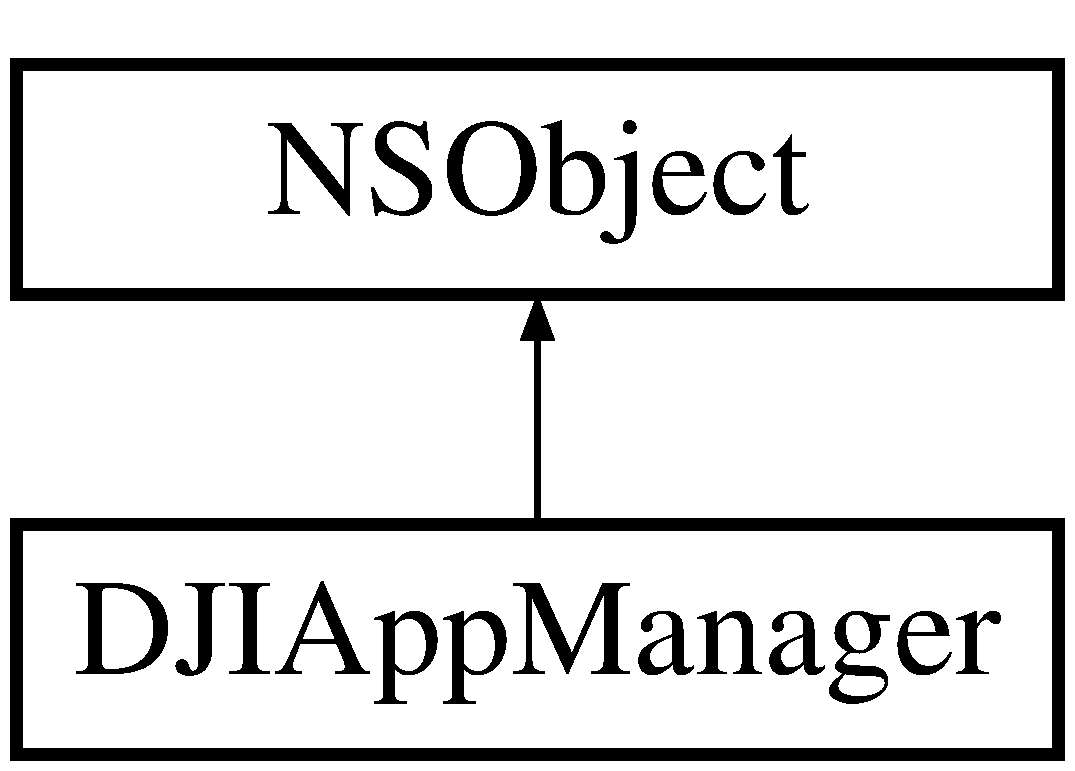
\includegraphics[height=2.000000cm]{interface_d_j_i_app_manager}
\end{center}
\end{figure}
\subsection*{Class Methods}
\begin{DoxyCompactItemize}
\item 
(void) + \hyperlink{interface_d_j_i_app_manager_a5fc2b9ae612f559639f631c7b1dfbf4e}{register\+App\+:with\+Delegate\+:}
\item 
(N\+S\+String $\ast$) + \hyperlink{interface_d_j_i_app_manager_adb0281179205bdd28ecb93dc5a0c482d}{get\+Error\+Descryption\+:}
\item 
(N\+S\+String $\ast$) + \hyperlink{interface_d_j_i_app_manager_af0ca386a7a26797da7c4806b016850b6}{get\+Framework\+Version}
\end{DoxyCompactItemize}


\subsection{Method Documentation}
\hypertarget{interface_d_j_i_app_manager_adb0281179205bdd28ecb93dc5a0c482d}{\index{D\+J\+I\+App\+Manager@{D\+J\+I\+App\+Manager}!get\+Error\+Descryption\+:@{get\+Error\+Descryption\+:}}
\index{get\+Error\+Descryption\+:@{get\+Error\+Descryption\+:}!D\+J\+I\+App\+Manager@{D\+J\+I\+App\+Manager}}
\subsubsection[{get\+Error\+Descryption\+:}]{\setlength{\rightskip}{0pt plus 5cm}+ (N\+S\+String$\ast$) get\+Error\+Descryption\+: 
\begin{DoxyParamCaption}
\item[{(int)}]{error\+Code}
\end{DoxyParamCaption}
}}\label{interface_d_j_i_app_manager_adb0281179205bdd28ecb93dc5a0c482d}
Get the detail descryption for the regist error code \hypertarget{interface_d_j_i_app_manager_af0ca386a7a26797da7c4806b016850b6}{\index{D\+J\+I\+App\+Manager@{D\+J\+I\+App\+Manager}!get\+Framework\+Version@{get\+Framework\+Version}}
\index{get\+Framework\+Version@{get\+Framework\+Version}!D\+J\+I\+App\+Manager@{D\+J\+I\+App\+Manager}}
\subsubsection[{get\+Framework\+Version}]{\setlength{\rightskip}{0pt plus 5cm}+ (N\+S\+String$\ast$) get\+Framework\+Version 
\begin{DoxyParamCaption}
{}
\end{DoxyParamCaption}
}}\label{interface_d_j_i_app_manager_af0ca386a7a26797da7c4806b016850b6}
Get D\+J\+I S\+D\+K framework version

\begin{DoxyReturn}{Returns}
Version 
\end{DoxyReturn}
\hypertarget{interface_d_j_i_app_manager_a5fc2b9ae612f559639f631c7b1dfbf4e}{\index{D\+J\+I\+App\+Manager@{D\+J\+I\+App\+Manager}!register\+App\+:with\+Delegate\+:@{register\+App\+:with\+Delegate\+:}}
\index{register\+App\+:with\+Delegate\+:@{register\+App\+:with\+Delegate\+:}!D\+J\+I\+App\+Manager@{D\+J\+I\+App\+Manager}}
\subsubsection[{register\+App\+:with\+Delegate\+:}]{\setlength{\rightskip}{0pt plus 5cm}+ (void) register\+App\+: 
\begin{DoxyParamCaption}
\item[{(N\+S\+String $\ast$)}]{app\+Key}
\item[{withDelegate:(id$<$ {\bf D\+J\+I\+App\+Manager\+Delegate} $>$)}]{delegate}
\end{DoxyParamCaption}
}}\label{interface_d_j_i_app_manager_a5fc2b9ae612f559639f631c7b1dfbf4e}
Register app from server. User should call once while app started and should connect to the internet at the first time register.


\begin{DoxyParams}{Parameters}
{\em app\+Key} & App key \\
\hline
{\em delegate} & Register result callback \\
\hline
\end{DoxyParams}


The documentation for this class was generated from the following file\+:\begin{DoxyCompactItemize}
\item 
D\+J\+I\+App\+Manager.\+h\end{DoxyCompactItemize}

\hypertarget{protocol_d_j_i_app_manager_delegate-p}{\section{$<$D\+J\+I\+App\+Manager\+Delegate$>$ Protocol Reference}
\label{protocol_d_j_i_app_manager_delegate-p}\index{$<$\+D\+J\+I\+App\+Manager\+Delegate$>$@{$<$\+D\+J\+I\+App\+Manager\+Delegate$>$}}
}
Inheritance diagram for $<$D\+J\+I\+App\+Manager\+Delegate$>$\+:\begin{figure}[H]
\begin{center}
\leavevmode
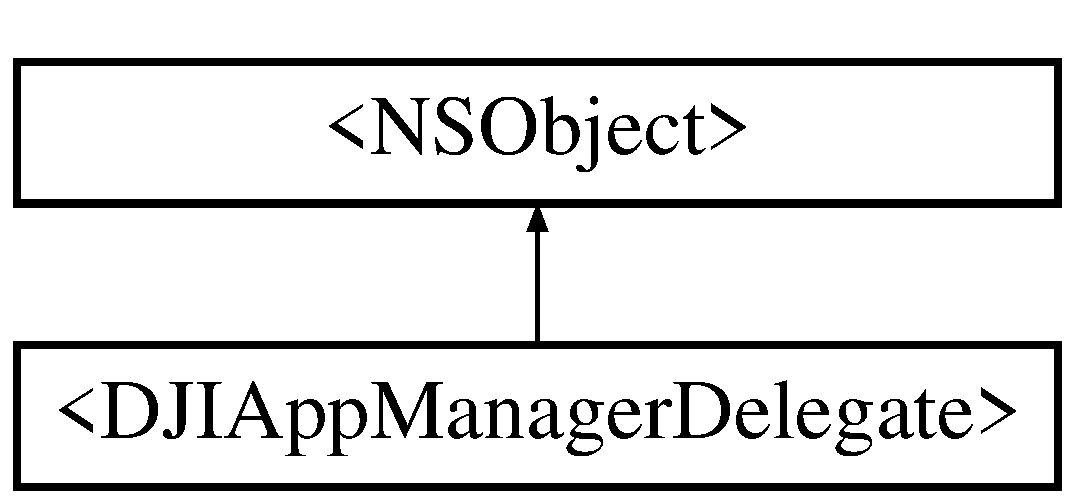
\includegraphics[height=2.000000cm]{protocol_d_j_i_app_manager_delegate-p}
\end{center}
\end{figure}
\subsection*{Instance Methods}
\begin{DoxyCompactItemize}
\item 
(void) -\/ \hyperlink{protocol_d_j_i_app_manager_delegate-p_a85c3839689b451e2e685e2c65bb7d655}{app\+Manager\+Did\+Register\+With\+Error\+:}
\end{DoxyCompactItemize}


\subsection{Method Documentation}
\hypertarget{protocol_d_j_i_app_manager_delegate-p_a85c3839689b451e2e685e2c65bb7d655}{\index{D\+J\+I\+App\+Manager\+Delegate-\/p@{D\+J\+I\+App\+Manager\+Delegate-\/p}!app\+Manager\+Did\+Register\+With\+Error\+:@{app\+Manager\+Did\+Register\+With\+Error\+:}}
\index{app\+Manager\+Did\+Register\+With\+Error\+:@{app\+Manager\+Did\+Register\+With\+Error\+:}!D\+J\+I\+App\+Manager\+Delegate-\/p@{D\+J\+I\+App\+Manager\+Delegate-\/p}}
\subsubsection[{app\+Manager\+Did\+Register\+With\+Error\+:}]{\setlength{\rightskip}{0pt plus 5cm}-\/ (void) app\+Manager\+Did\+Register\+With\+Error\+: 
\begin{DoxyParamCaption}
\item[{(int)}]{error\+Code}
\end{DoxyParamCaption}
}}\label{protocol_d_j_i_app_manager_delegate-p_a85c3839689b451e2e685e2c65bb7d655}
Register result 

The documentation for this protocol was generated from the following file\+:\begin{DoxyCompactItemize}
\item 
D\+J\+I\+App\+Manager.\+h\end{DoxyCompactItemize}

\hypertarget{struct_d_j_i_attitude}{\section{D\+J\+I\+Attitude Struct Reference}
\label{struct_d_j_i_attitude}\index{D\+J\+I\+Attitude@{D\+J\+I\+Attitude}}
}
\subsection*{Protected Attributes}
\begin{DoxyCompactItemize}
\item 
\hypertarget{struct_d_j_i_attitude_a06da02bd519fc651963b84e6adda34df}{double {\bfseries pitch}}\label{struct_d_j_i_attitude_a06da02bd519fc651963b84e6adda34df}

\item 
\hypertarget{struct_d_j_i_attitude_a5b24feb9c501776a0d129a151ffaa6f9}{double {\bfseries roll}}\label{struct_d_j_i_attitude_a5b24feb9c501776a0d129a151ffaa6f9}

\item 
\hypertarget{struct_d_j_i_attitude_aeb6af3357a98e570e19564d2e3787017}{double {\bfseries yaw}}\label{struct_d_j_i_attitude_aeb6af3357a98e570e19564d2e3787017}

\end{DoxyCompactItemize}


The documentation for this struct was generated from the following file\+:\begin{DoxyCompactItemize}
\item 
D\+J\+I\+Main\+Controller.\+h\end{DoxyCompactItemize}

\hypertarget{interface_d_j_i_battery}{\section{D\+J\+I\+Battery Class Reference}
\label{interface_d_j_i_battery}\index{D\+J\+I\+Battery@{D\+J\+I\+Battery}}
}
Inheritance diagram for D\+J\+I\+Battery\+:\begin{figure}[H]
\begin{center}
\leavevmode
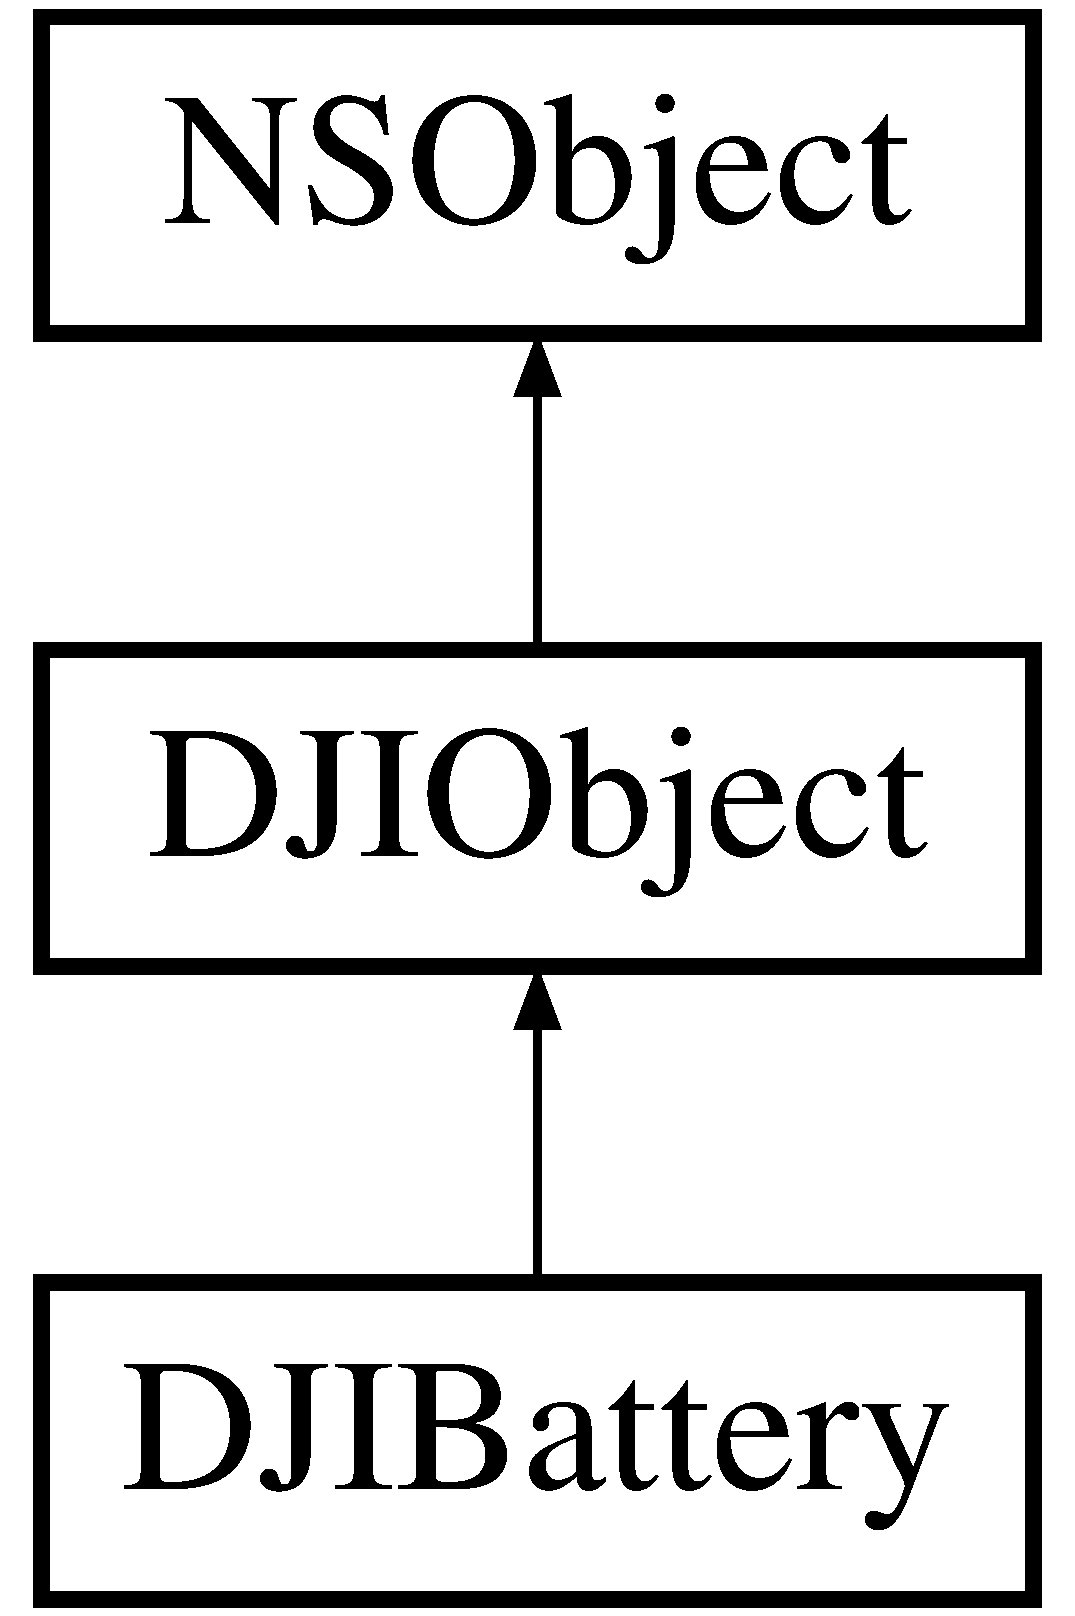
\includegraphics[height=3.000000cm]{interface_d_j_i_battery}
\end{center}
\end{figure}
\subsection*{Instance Methods}
\begin{DoxyCompactItemize}
\item 
(void) -\/ \hyperlink{interface_d_j_i_battery_a5e3bd4fe2ad55e276cf14c7624928307}{update\+Battery\+Info\+:}
\end{DoxyCompactItemize}
\subsection*{Properties}
\begin{DoxyCompactItemize}
\item 
N\+S\+Integer \hyperlink{interface_d_j_i_battery_a37e3119e928eaac82f3670cacd3b191e}{designed\+Volume}
\item 
N\+S\+Integer \hyperlink{interface_d_j_i_battery_a87e103436cc4f431bbdc1928cb966326}{full\+Charge\+Volume}
\item 
N\+S\+Integer \hyperlink{interface_d_j_i_battery_a9e00083e9a8276841941d13878dd0280}{current\+Electricity}
\item 
N\+S\+Integer \hyperlink{interface_d_j_i_battery_a2cdaf2d785248e9ce20908bed4fbd2a9}{current\+Voltage}
\item 
N\+S\+Integer \hyperlink{interface_d_j_i_battery_a15cb9aa7a65f755d4822a1bbfd095496}{current\+Current}
\item 
N\+S\+Integer \hyperlink{interface_d_j_i_battery_a254d1b5afd5e99b82f8d18598b840b8f}{remain\+Life\+Percent}
\item 
N\+S\+Integer \hyperlink{interface_d_j_i_battery_a79eeca54fbd09a177ae67d1173d70396}{remain\+Power\+Percent}
\item 
N\+S\+Integer \hyperlink{interface_d_j_i_battery_a592f495cbb583ec4aa4a1323605f53b0}{battery\+Temperature}
\item 
N\+S\+Integer \hyperlink{interface_d_j_i_battery_a5f1acd23e4218474087ef29e2b8c3bb3}{discharge\+Count}
\end{DoxyCompactItemize}


\subsection{Method Documentation}
\hypertarget{interface_d_j_i_battery_a5e3bd4fe2ad55e276cf14c7624928307}{\index{D\+J\+I\+Battery@{D\+J\+I\+Battery}!update\+Battery\+Info\+:@{update\+Battery\+Info\+:}}
\index{update\+Battery\+Info\+:@{update\+Battery\+Info\+:}!D\+J\+I\+Battery@{D\+J\+I\+Battery}}
\subsubsection[{update\+Battery\+Info\+:}]{\setlength{\rightskip}{0pt plus 5cm}-\/ (void) update\+Battery\+Info\+: 
\begin{DoxyParamCaption}
\item[{(D\+J\+I\+Execute\+Result\+Block)}]{block}
\end{DoxyParamCaption}
}}\label{interface_d_j_i_battery_a5e3bd4fe2ad55e276cf14c7624928307}
update battery information


\begin{DoxyParams}{Parameters}
{\em block} & Remote exeucte result \\
\hline
\end{DoxyParams}


\subsection{Property Documentation}
\hypertarget{interface_d_j_i_battery_a592f495cbb583ec4aa4a1323605f53b0}{\index{D\+J\+I\+Battery@{D\+J\+I\+Battery}!battery\+Temperature@{battery\+Temperature}}
\index{battery\+Temperature@{battery\+Temperature}!D\+J\+I\+Battery@{D\+J\+I\+Battery}}
\subsubsection[{battery\+Temperature}]{\setlength{\rightskip}{0pt plus 5cm}-\/ (N\+S\+Integer) battery\+Temperature\hspace{0.3cm}{\ttfamily [read]}, {\ttfamily [write]}, {\ttfamily [nonatomic]}, {\ttfamily [assign]}}}\label{interface_d_j_i_battery_a592f495cbb583ec4aa4a1323605f53b0}
temperature between -\/128 to 127 (Centigrade) \hypertarget{interface_d_j_i_battery_a15cb9aa7a65f755d4822a1bbfd095496}{\index{D\+J\+I\+Battery@{D\+J\+I\+Battery}!current\+Current@{current\+Current}}
\index{current\+Current@{current\+Current}!D\+J\+I\+Battery@{D\+J\+I\+Battery}}
\subsubsection[{current\+Current}]{\setlength{\rightskip}{0pt plus 5cm}-\/ (N\+S\+Integer) current\+Current\hspace{0.3cm}{\ttfamily [read]}, {\ttfamily [write]}, {\ttfamily [nonatomic]}, {\ttfamily [assign]}}}\label{interface_d_j_i_battery_a15cb9aa7a65f755d4822a1bbfd095496}
current (m\+A) \hypertarget{interface_d_j_i_battery_a9e00083e9a8276841941d13878dd0280}{\index{D\+J\+I\+Battery@{D\+J\+I\+Battery}!current\+Electricity@{current\+Electricity}}
\index{current\+Electricity@{current\+Electricity}!D\+J\+I\+Battery@{D\+J\+I\+Battery}}
\subsubsection[{current\+Electricity}]{\setlength{\rightskip}{0pt plus 5cm}-\/ (N\+S\+Integer) current\+Electricity\hspace{0.3cm}{\ttfamily [read]}, {\ttfamily [write]}, {\ttfamily [nonatomic]}, {\ttfamily [assign]}}}\label{interface_d_j_i_battery_a9e00083e9a8276841941d13878dd0280}
current electricity volume (m\+Ah) \hypertarget{interface_d_j_i_battery_a2cdaf2d785248e9ce20908bed4fbd2a9}{\index{D\+J\+I\+Battery@{D\+J\+I\+Battery}!current\+Voltage@{current\+Voltage}}
\index{current\+Voltage@{current\+Voltage}!D\+J\+I\+Battery@{D\+J\+I\+Battery}}
\subsubsection[{current\+Voltage}]{\setlength{\rightskip}{0pt plus 5cm}-\/ (N\+S\+Integer) current\+Voltage\hspace{0.3cm}{\ttfamily [read]}, {\ttfamily [write]}, {\ttfamily [nonatomic]}, {\ttfamily [assign]}}}\label{interface_d_j_i_battery_a2cdaf2d785248e9ce20908bed4fbd2a9}
voltage (m\+V) \hypertarget{interface_d_j_i_battery_a37e3119e928eaac82f3670cacd3b191e}{\index{D\+J\+I\+Battery@{D\+J\+I\+Battery}!designed\+Volume@{designed\+Volume}}
\index{designed\+Volume@{designed\+Volume}!D\+J\+I\+Battery@{D\+J\+I\+Battery}}
\subsubsection[{designed\+Volume}]{\setlength{\rightskip}{0pt plus 5cm}-\/ (N\+S\+Integer) designed\+Volume\hspace{0.3cm}{\ttfamily [read]}, {\ttfamily [write]}, {\ttfamily [nonatomic]}, {\ttfamily [assign]}}}\label{interface_d_j_i_battery_a37e3119e928eaac82f3670cacd3b191e}
the battery's design volume (m\+Ah) \hypertarget{interface_d_j_i_battery_a5f1acd23e4218474087ef29e2b8c3bb3}{\index{D\+J\+I\+Battery@{D\+J\+I\+Battery}!discharge\+Count@{discharge\+Count}}
\index{discharge\+Count@{discharge\+Count}!D\+J\+I\+Battery@{D\+J\+I\+Battery}}
\subsubsection[{discharge\+Count}]{\setlength{\rightskip}{0pt plus 5cm}-\/ (N\+S\+Integer) discharge\+Count\hspace{0.3cm}{\ttfamily [read]}, {\ttfamily [write]}, {\ttfamily [nonatomic]}, {\ttfamily [assign]}}}\label{interface_d_j_i_battery_a5f1acd23e4218474087ef29e2b8c3bb3}
the history discharge count \hypertarget{interface_d_j_i_battery_a87e103436cc4f431bbdc1928cb966326}{\index{D\+J\+I\+Battery@{D\+J\+I\+Battery}!full\+Charge\+Volume@{full\+Charge\+Volume}}
\index{full\+Charge\+Volume@{full\+Charge\+Volume}!D\+J\+I\+Battery@{D\+J\+I\+Battery}}
\subsubsection[{full\+Charge\+Volume}]{\setlength{\rightskip}{0pt plus 5cm}-\/ (N\+S\+Integer) full\+Charge\+Volume\hspace{0.3cm}{\ttfamily [read]}, {\ttfamily [write]}, {\ttfamily [nonatomic]}, {\ttfamily [assign]}}}\label{interface_d_j_i_battery_a87e103436cc4f431bbdc1928cb966326}
the battery's full charge volume (m\+Ah) \hypertarget{interface_d_j_i_battery_a254d1b5afd5e99b82f8d18598b840b8f}{\index{D\+J\+I\+Battery@{D\+J\+I\+Battery}!remain\+Life\+Percent@{remain\+Life\+Percent}}
\index{remain\+Life\+Percent@{remain\+Life\+Percent}!D\+J\+I\+Battery@{D\+J\+I\+Battery}}
\subsubsection[{remain\+Life\+Percent}]{\setlength{\rightskip}{0pt plus 5cm}-\/ (N\+S\+Integer) remain\+Life\+Percent\hspace{0.3cm}{\ttfamily [read]}, {\ttfamily [write]}, {\ttfamily [nonatomic]}, {\ttfamily [assign]}}}\label{interface_d_j_i_battery_a254d1b5afd5e99b82f8d18598b840b8f}
remain life percentage \hypertarget{interface_d_j_i_battery_a79eeca54fbd09a177ae67d1173d70396}{\index{D\+J\+I\+Battery@{D\+J\+I\+Battery}!remain\+Power\+Percent@{remain\+Power\+Percent}}
\index{remain\+Power\+Percent@{remain\+Power\+Percent}!D\+J\+I\+Battery@{D\+J\+I\+Battery}}
\subsubsection[{remain\+Power\+Percent}]{\setlength{\rightskip}{0pt plus 5cm}-\/ (N\+S\+Integer) remain\+Power\+Percent\hspace{0.3cm}{\ttfamily [read]}, {\ttfamily [write]}, {\ttfamily [nonatomic]}, {\ttfamily [assign]}}}\label{interface_d_j_i_battery_a79eeca54fbd09a177ae67d1173d70396}
remain power percentage 

The documentation for this class was generated from the following file\+:\begin{DoxyCompactItemize}
\item 
D\+J\+I\+Battery.\+h\end{DoxyCompactItemize}

\hypertarget{interface_d_j_i_camera}{\section{D\+J\+I\+Camera Class Reference}
\label{interface_d_j_i_camera}\index{D\+J\+I\+Camera@{D\+J\+I\+Camera}}
}
Inheritance diagram for D\+J\+I\+Camera\+:\begin{figure}[H]
\begin{center}
\leavevmode
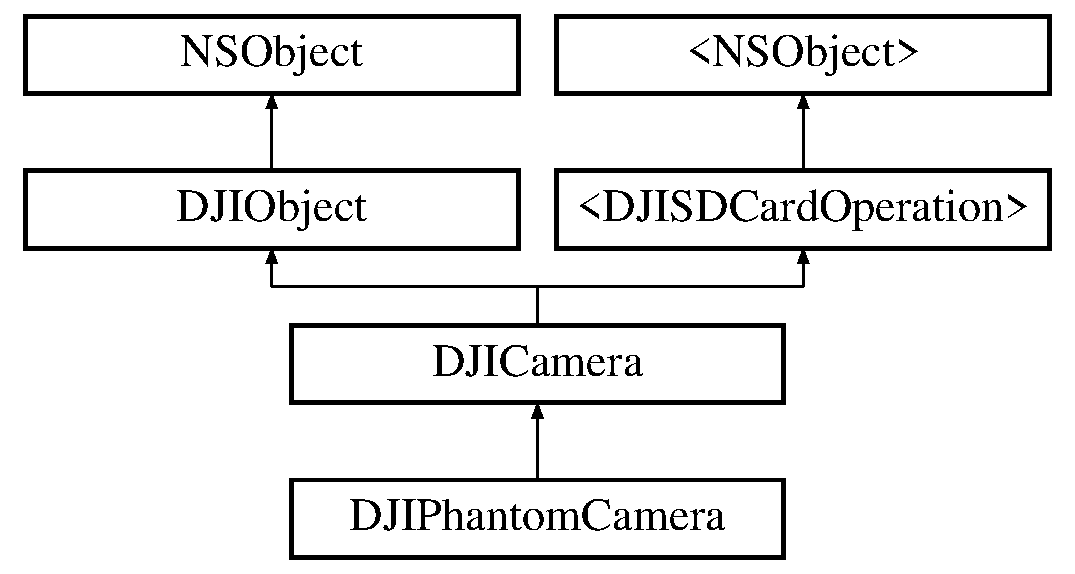
\includegraphics[height=4.000000cm]{interface_d_j_i_camera}
\end{center}
\end{figure}
\subsection*{Instance Methods}
\begin{DoxyCompactItemize}
\item 
(N\+S\+String $\ast$) -\/ \hyperlink{interface_d_j_i_camera_a7c2320f498ee70afef23423f8f0d1d31}{get\+Camera\+Version}
\item 
(void) -\/ \hyperlink{interface_d_j_i_camera_a090650e2871815020f6173d896aa78be}{start\+Take\+Photo\+:with\+Result\+:}
\item 
(void) -\/ \hyperlink{interface_d_j_i_camera_a0ece0c556f5c761bb719b60b29035779}{stop\+Take\+Photo\+With\+Result\+:}
\item 
(void) -\/ \hyperlink{interface_d_j_i_camera_a4619149cc2aedaf0553925ddd3c9ffa5}{start\+Record\+:}
\item 
(void) -\/ \hyperlink{interface_d_j_i_camera_ab5b94d6306cfb45412f1bd437a5309ce}{stop\+Record\+:}
\item 
(void) -\/ \hyperlink{interface_d_j_i_camera_a53ae8c880028f6f386a91b7b7ad32e1c}{start\+Camera\+System\+State\+Updates}
\item 
(void) -\/ \hyperlink{interface_d_j_i_camera_a866b64532676176a7a1b8eb890b188d8}{stop\+Camera\+System\+State\+Updates}
\item 
(void) -\/ \hyperlink{interface_d_j_i_camera_a056998f58df4c307417929683cd56066}{set\+Video\+Quality\+:with\+Result\+Block\+:}
\item 
(void) -\/ \hyperlink{interface_d_j_i_camera_a0b0183eed1dbf991ce49942f32e78a4b}{set\+Camera\+Photo\+Size\+:with\+Result\+Block\+:}
\item 
(void) -\/ \hyperlink{interface_d_j_i_camera_a3bb87caf5b5f9d3810cb4bad9cc15075}{get\+Camera\+Photo\+Size\+:}
\item 
(void) -\/ \hyperlink{interface_d_j_i_camera_a50e4e75ec9ed1bdac6a058fc36820f77}{set\+Camera\+I\+S\+O\+:with\+Result\+Block\+:}
\item 
(void) -\/ \hyperlink{interface_d_j_i_camera_a9b98d7b6e1f51e1087fed5e514bb9a3d}{get\+Camera\+I\+S\+O\+:}
\item 
(void) -\/ \hyperlink{interface_d_j_i_camera_a196c669179c9c9cf02ef2b554f56081d}{set\+Camera\+White\+Balance\+:with\+Result\+Block\+:}
\item 
(void) -\/ \hyperlink{interface_d_j_i_camera_a1b0a2c1fdbb4b01e1881b48f11355d86}{get\+Camera\+White\+Balance\+:}
\item 
(void) -\/ \hyperlink{interface_d_j_i_camera_ada2dace1e4513d0fa39e99e9e80d32fc}{set\+Camera\+Exposure\+Metering\+:with\+Result\+Block\+:}
\item 
(void) -\/ \hyperlink{interface_d_j_i_camera_a2bf7db98f17444eb1237a3e15876dbc9}{get\+Camera\+Exposure\+Metering\+:}
\item 
(void) -\/ \hyperlink{interface_d_j_i_camera_ab31e7fceb02ab8297592c0237178c124}{set\+Camera\+Recording\+Resolution\+:and\+F\+O\+V\+:with\+Result\+Block\+:}
\item 
(void) -\/ \hyperlink{interface_d_j_i_camera_abf7a4e534fca76520b6b7723b267b33c}{get\+Camera\+Recording\+Resolution\+:}
\item 
(void) -\/ \hyperlink{interface_d_j_i_camera_a866646cab142e602d5c41074c7931b26}{set\+Camera\+Photo\+Format\+:with\+Result\+Block\+:}
\item 
(void) -\/ \hyperlink{interface_d_j_i_camera_aacb8e2260944d9bc5d02840dbd98952f}{get\+Camera\+Photo\+Format\+:}
\item 
(void) -\/ \hyperlink{interface_d_j_i_camera_a6755ae71cfba5edd7ead0132d2e8b32a}{set\+Camera\+Exposure\+Compensation\+:with\+Result\+Block\+:}
\item 
(void) -\/ \hyperlink{interface_d_j_i_camera_a8ac02ef272b0748ae0b9ba0606cf1ff5}{get\+Camera\+Exposure\+Compensation\+:}
\item 
(void) -\/ \hyperlink{interface_d_j_i_camera_a6de121d0c2f5380a3f981ab58fd3d039}{set\+Camera\+Anti\+Flicker\+:with\+Result\+Block\+:}
\item 
(void) -\/ \hyperlink{interface_d_j_i_camera_a8a10b5f222f52ab4a567f9daaa66c01b}{get\+Camera\+Anti\+Flicker\+:}
\item 
(void) -\/ \hyperlink{interface_d_j_i_camera_a3e12cf84035bd62ed1ed0c8b631744b0}{set\+Camera\+Sharpness\+:with\+Result\+Block\+:}
\item 
(void) -\/ \hyperlink{interface_d_j_i_camera_ac66a941aa97f5759b6edbeed63ed2651}{get\+Camera\+Sharpness\+:}
\item 
(void) -\/ \hyperlink{interface_d_j_i_camera_a0f6dc6fba1427b888eef36be70d3a66b}{set\+Camera\+Contrast\+:with\+Result\+Block\+:}
\item 
(void) -\/ \hyperlink{interface_d_j_i_camera_a808873449e7ee9d0cd934717c8da5d56}{get\+Camera\+Contrast\+:}
\item 
(void) -\/ \hyperlink{interface_d_j_i_camera_a859dae115d90d5a76b9bb20ff7472ad3}{sync\+Time\+:}
\item 
(void) -\/ \hyperlink{interface_d_j_i_camera_ab82f5dd8ff7436ff1854e87b8d98dd32}{set\+Camera\+Gps\+:with\+Result\+Block\+:}
\item 
(void) -\/ \hyperlink{interface_d_j_i_camera_a12ea90b2078c79e442b737367f174d69}{get\+Camera\+Gps\+:}
\item 
(void) -\/ \hyperlink{interface_d_j_i_camera_a24deec8c2d2c3400fb429d3970b118a8}{set\+Multi\+Capture\+Count\+:with\+Result\+Block\+:}
\item 
(void) -\/ \hyperlink{interface_d_j_i_camera_aadf6c311c34ca3350c499ffebfa56360}{get\+Multi\+Capture\+Count\+:}
\item 
(void) -\/ \hyperlink{interface_d_j_i_camera_a1778f87e60ea80287eeac26bc5ce20c1}{set\+Continuous\+Capture\+:with\+Result\+Block\+:}
\item 
(void) -\/ \hyperlink{interface_d_j_i_camera_a24a0b6d29efc68288434cc7f8dd9820a}{get\+Continuous\+Capture\+Param\+:}
\item 
(void) -\/ \hyperlink{interface_d_j_i_camera_a71e8465d77880dbd1e6503b1c053a3c8}{set\+Camera\+Action\+When\+Connection\+Broken\+:with\+Result\+Block\+:}
\item 
(void) -\/ \hyperlink{interface_d_j_i_camera_ad0a73beaa9c1a8f4d3f671cd502709a4}{get\+Camera\+Action\+When\+Connection\+Broken\+:}
\item 
(void) -\/ \hyperlink{interface_d_j_i_camera_a6ecf06b591c070b0802c750e146a7083}{save\+Camera\+Settings\+:}
\item 
(void) -\/ \hyperlink{interface_d_j_i_camera_ae9dfbd7729c65f2c2b38375a31741945}{restore\+Camera\+Default\+Settings\+:}
\item 
(void) -\/ \hyperlink{interface_d_j_i_camera_a9c3024a4d659577b916421429a9ed1fe}{set\+Camer\+Mode\+:with\+Result\+Block\+:}
\item 
(void) -\/ \hyperlink{interface_d_j_i_camera_aa7aa0fa592b6b7ffdd403308e7896f71}{get\+Camera\+Photo\+Name\+Prefix\+:}
\item 
(void) -\/ \hyperlink{interface_d_j_i_camera_a9825d0b6c5f400877d1d8761fdd0de57}{set\+Camera\+Photo\+Name\+Prefix\+:with\+Result\+Block\+:}
\item 
(void) -\/ \hyperlink{interface_d_j_i_camera_aec60d27962d501aacd4a1324adca0775}{fetch\+Media\+List\+With\+Result\+Block\+:}
\end{DoxyCompactItemize}
\subsection*{Properties}
\begin{DoxyCompactItemize}
\item 
\hypertarget{interface_d_j_i_camera_a7b8c8c19d3041aac44699c37ac94a784}{id$<$ \hyperlink{protocol_d_j_i_camera_delegate-p}{D\+J\+I\+Camera\+Delegate} $>$ {\bfseries delegate}}\label{interface_d_j_i_camera_a7b8c8c19d3041aac44699c37ac94a784}

\end{DoxyCompactItemize}


\subsection{Method Documentation}
\hypertarget{interface_d_j_i_camera_aec60d27962d501aacd4a1324adca0775}{\index{D\+J\+I\+Camera@{D\+J\+I\+Camera}!fetch\+Media\+List\+With\+Result\+Block\+:@{fetch\+Media\+List\+With\+Result\+Block\+:}}
\index{fetch\+Media\+List\+With\+Result\+Block\+:@{fetch\+Media\+List\+With\+Result\+Block\+:}!D\+J\+I\+Camera@{D\+J\+I\+Camera}}
\subsubsection[{fetch\+Media\+List\+With\+Result\+Block\+:}]{\setlength{\rightskip}{0pt plus 5cm}-\/ (void) fetch\+Media\+List\+With\+Result\+Block\+: 
\begin{DoxyParamCaption}
\item[{(void($^\wedge$)(N\+S\+Array $\ast$media\+List, N\+S\+Error $\ast$error))}]{block}
\end{DoxyParamCaption}
}}\label{interface_d_j_i_camera_aec60d27962d501aacd4a1324adca0775}
Fetch media list from remote album.


\begin{DoxyParams}{Parameters}
{\em block} & The remote execute result block \\
\hline
\end{DoxyParams}
\begin{DoxyAttention}{Attention}
The camera mode should be set as 'Camera\+U\+S\+B\+Mode'. 
\end{DoxyAttention}


Provided by category \hyperlink{category_d_j_i_camera_07_media_08_aec60d27962d501aacd4a1324adca0775}{D\+J\+I\+Camera(\+Media)}.

\hypertarget{interface_d_j_i_camera_ad0a73beaa9c1a8f4d3f671cd502709a4}{\index{D\+J\+I\+Camera@{D\+J\+I\+Camera}!get\+Camera\+Action\+When\+Connection\+Broken\+:@{get\+Camera\+Action\+When\+Connection\+Broken\+:}}
\index{get\+Camera\+Action\+When\+Connection\+Broken\+:@{get\+Camera\+Action\+When\+Connection\+Broken\+:}!D\+J\+I\+Camera@{D\+J\+I\+Camera}}
\subsubsection[{get\+Camera\+Action\+When\+Connection\+Broken\+:}]{\setlength{\rightskip}{0pt plus 5cm}-\/ (void) get\+Camera\+Action\+When\+Connection\+Broken\+: 
\begin{DoxyParamCaption}
\item[{(void($^\wedge$)(Camera\+Action\+When\+Break camera\+Action, {\bf D\+J\+I\+Error} $\ast$error))}]{block}
\end{DoxyParamCaption}
}}\label{interface_d_j_i_camera_ad0a73beaa9c1a8f4d3f671cd502709a4}
Get the camera's action settings while the connection was broken.


\begin{DoxyParams}{Parameters}
{\em block} & The remote execute result block \\
\hline
\end{DoxyParams}


Provided by category \hyperlink{category_d_j_i_camera_07_camera_settings_08_ad0a73beaa9c1a8f4d3f671cd502709a4}{D\+J\+I\+Camera(\+Camera\+Settings)}.

\hypertarget{interface_d_j_i_camera_a8a10b5f222f52ab4a567f9daaa66c01b}{\index{D\+J\+I\+Camera@{D\+J\+I\+Camera}!get\+Camera\+Anti\+Flicker\+:@{get\+Camera\+Anti\+Flicker\+:}}
\index{get\+Camera\+Anti\+Flicker\+:@{get\+Camera\+Anti\+Flicker\+:}!D\+J\+I\+Camera@{D\+J\+I\+Camera}}
\subsubsection[{get\+Camera\+Anti\+Flicker\+:}]{\setlength{\rightskip}{0pt plus 5cm}-\/ (void) get\+Camera\+Anti\+Flicker\+: 
\begin{DoxyParamCaption}
\item[{(void($^\wedge$)(Camera\+Anti\+Flicker\+Type anti\+Flicker, {\bf D\+J\+I\+Error} $\ast$error))}]{block}
\end{DoxyParamCaption}
}}\label{interface_d_j_i_camera_a8a10b5f222f52ab4a567f9daaa66c01b}
Get the camera's anti flicker parameter


\begin{DoxyParams}{Parameters}
{\em block} & The remote execute result block \\
\hline
\end{DoxyParams}


Provided by category \hyperlink{category_d_j_i_camera_07_camera_settings_08_a8a10b5f222f52ab4a567f9daaa66c01b}{D\+J\+I\+Camera(\+Camera\+Settings)}.

\hypertarget{interface_d_j_i_camera_a808873449e7ee9d0cd934717c8da5d56}{\index{D\+J\+I\+Camera@{D\+J\+I\+Camera}!get\+Camera\+Contrast\+:@{get\+Camera\+Contrast\+:}}
\index{get\+Camera\+Contrast\+:@{get\+Camera\+Contrast\+:}!D\+J\+I\+Camera@{D\+J\+I\+Camera}}
\subsubsection[{get\+Camera\+Contrast\+:}]{\setlength{\rightskip}{0pt plus 5cm}-\/ (void) get\+Camera\+Contrast\+: 
\begin{DoxyParamCaption}
\item[{(void($^\wedge$)(Camera\+Contrast\+Type contrast, {\bf D\+J\+I\+Error} $\ast$error))}]{block}
\end{DoxyParamCaption}
}}\label{interface_d_j_i_camera_a808873449e7ee9d0cd934717c8da5d56}
Get camera contrast


\begin{DoxyParams}{Parameters}
{\em block} & The remote execute result block \\
\hline
\end{DoxyParams}


Provided by category \hyperlink{category_d_j_i_camera_07_camera_settings_08_a808873449e7ee9d0cd934717c8da5d56}{D\+J\+I\+Camera(\+Camera\+Settings)}.

\hypertarget{interface_d_j_i_camera_a8ac02ef272b0748ae0b9ba0606cf1ff5}{\index{D\+J\+I\+Camera@{D\+J\+I\+Camera}!get\+Camera\+Exposure\+Compensation\+:@{get\+Camera\+Exposure\+Compensation\+:}}
\index{get\+Camera\+Exposure\+Compensation\+:@{get\+Camera\+Exposure\+Compensation\+:}!D\+J\+I\+Camera@{D\+J\+I\+Camera}}
\subsubsection[{get\+Camera\+Exposure\+Compensation\+:}]{\setlength{\rightskip}{0pt plus 5cm}-\/ (void) get\+Camera\+Exposure\+Compensation\+: 
\begin{DoxyParamCaption}
\item[{(void($^\wedge$)(Camera\+Exposure\+Compensation\+Type exposure\+Compensation, {\bf D\+J\+I\+Error} $\ast$error))}]{block}
\end{DoxyParamCaption}
}}\label{interface_d_j_i_camera_a8ac02ef272b0748ae0b9ba0606cf1ff5}
Get camera's exposure compensation


\begin{DoxyParams}{Parameters}
{\em block} & The remote execute result block \\
\hline
\end{DoxyParams}


Provided by category \hyperlink{category_d_j_i_camera_07_camera_settings_08_a8ac02ef272b0748ae0b9ba0606cf1ff5}{D\+J\+I\+Camera(\+Camera\+Settings)}.

\hypertarget{interface_d_j_i_camera_a2bf7db98f17444eb1237a3e15876dbc9}{\index{D\+J\+I\+Camera@{D\+J\+I\+Camera}!get\+Camera\+Exposure\+Metering\+:@{get\+Camera\+Exposure\+Metering\+:}}
\index{get\+Camera\+Exposure\+Metering\+:@{get\+Camera\+Exposure\+Metering\+:}!D\+J\+I\+Camera@{D\+J\+I\+Camera}}
\subsubsection[{get\+Camera\+Exposure\+Metering\+:}]{\setlength{\rightskip}{0pt plus 5cm}-\/ (void) get\+Camera\+Exposure\+Metering\+: 
\begin{DoxyParamCaption}
\item[{(void($^\wedge$)(Camera\+Exposure\+Metering\+Type exposure\+Metering, {\bf D\+J\+I\+Error} $\ast$error))}]{block}
\end{DoxyParamCaption}
}}\label{interface_d_j_i_camera_a2bf7db98f17444eb1237a3e15876dbc9}
Get the camera's exposure metering parameter


\begin{DoxyParams}{Parameters}
{\em block} & The remote execute result block \\
\hline
\end{DoxyParams}


Provided by category \hyperlink{category_d_j_i_camera_07_camera_settings_08_a2bf7db98f17444eb1237a3e15876dbc9}{D\+J\+I\+Camera(\+Camera\+Settings)}.

\hypertarget{interface_d_j_i_camera_a12ea90b2078c79e442b737367f174d69}{\index{D\+J\+I\+Camera@{D\+J\+I\+Camera}!get\+Camera\+Gps\+:@{get\+Camera\+Gps\+:}}
\index{get\+Camera\+Gps\+:@{get\+Camera\+Gps\+:}!D\+J\+I\+Camera@{D\+J\+I\+Camera}}
\subsubsection[{get\+Camera\+Gps\+:}]{\setlength{\rightskip}{0pt plus 5cm}-\/ (void) get\+Camera\+Gps\+: 
\begin{DoxyParamCaption}
\item[{(void($^\wedge$)(C\+L\+Location\+Coordinate2\+D coordinate, {\bf D\+J\+I\+Error} $\ast$error))}]{block}
\end{DoxyParamCaption}
}}\label{interface_d_j_i_camera_a12ea90b2078c79e442b737367f174d69}
Get the camera's G\+P\+S


\begin{DoxyParams}{Parameters}
{\em block} & The remote execute result block \\
\hline
\end{DoxyParams}


Provided by category \hyperlink{category_d_j_i_camera_07_camera_settings_08_a12ea90b2078c79e442b737367f174d69}{D\+J\+I\+Camera(\+Camera\+Settings)}.

\hypertarget{interface_d_j_i_camera_a9b98d7b6e1f51e1087fed5e514bb9a3d}{\index{D\+J\+I\+Camera@{D\+J\+I\+Camera}!get\+Camera\+I\+S\+O\+:@{get\+Camera\+I\+S\+O\+:}}
\index{get\+Camera\+I\+S\+O\+:@{get\+Camera\+I\+S\+O\+:}!D\+J\+I\+Camera@{D\+J\+I\+Camera}}
\subsubsection[{get\+Camera\+I\+S\+O\+:}]{\setlength{\rightskip}{0pt plus 5cm}-\/ (void) get\+Camera\+I\+S\+O\+: 
\begin{DoxyParamCaption}
\item[{(void($^\wedge$)(Camera\+I\+S\+O\+Type iso, {\bf D\+J\+I\+Error} $\ast$error))}]{block}
\end{DoxyParamCaption}
}}\label{interface_d_j_i_camera_a9b98d7b6e1f51e1087fed5e514bb9a3d}
Get the camera's I\+S\+O


\begin{DoxyParams}{Parameters}
{\em block} & The remote execute result block \\
\hline
\end{DoxyParams}


Provided by category \hyperlink{category_d_j_i_camera_07_camera_settings_08_a9b98d7b6e1f51e1087fed5e514bb9a3d}{D\+J\+I\+Camera(\+Camera\+Settings)}.

\hypertarget{interface_d_j_i_camera_aacb8e2260944d9bc5d02840dbd98952f}{\index{D\+J\+I\+Camera@{D\+J\+I\+Camera}!get\+Camera\+Photo\+Format\+:@{get\+Camera\+Photo\+Format\+:}}
\index{get\+Camera\+Photo\+Format\+:@{get\+Camera\+Photo\+Format\+:}!D\+J\+I\+Camera@{D\+J\+I\+Camera}}
\subsubsection[{get\+Camera\+Photo\+Format\+:}]{\setlength{\rightskip}{0pt plus 5cm}-\/ (void) get\+Camera\+Photo\+Format\+: 
\begin{DoxyParamCaption}
\item[{(void($^\wedge$)(Camera\+Photo\+Format\+Type photo\+Format, {\bf D\+J\+I\+Error} $\ast$error))}]{block}
\end{DoxyParamCaption}
}}\label{interface_d_j_i_camera_aacb8e2260944d9bc5d02840dbd98952f}
Get the camera's photo storage format


\begin{DoxyParams}{Parameters}
{\em block} & The remote execute result block \\
\hline
\end{DoxyParams}


Provided by category \hyperlink{category_d_j_i_camera_07_camera_settings_08_aacb8e2260944d9bc5d02840dbd98952f}{D\+J\+I\+Camera(\+Camera\+Settings)}.

\hypertarget{interface_d_j_i_camera_aa7aa0fa592b6b7ffdd403308e7896f71}{\index{D\+J\+I\+Camera@{D\+J\+I\+Camera}!get\+Camera\+Photo\+Name\+Prefix\+:@{get\+Camera\+Photo\+Name\+Prefix\+:}}
\index{get\+Camera\+Photo\+Name\+Prefix\+:@{get\+Camera\+Photo\+Name\+Prefix\+:}!D\+J\+I\+Camera@{D\+J\+I\+Camera}}
\subsubsection[{get\+Camera\+Photo\+Name\+Prefix\+:}]{\setlength{\rightskip}{0pt plus 5cm}-\/ (void) get\+Camera\+Photo\+Name\+Prefix\+: 
\begin{DoxyParamCaption}
\item[{(void($^\wedge$)(N\+S\+String $\ast$prefix, {\bf D\+J\+I\+Error} $\ast$error))}]{block}
\end{DoxyParamCaption}
}}\label{interface_d_j_i_camera_aa7aa0fa592b6b7ffdd403308e7896f71}
Get the camera's photo name prefix


\begin{DoxyParams}{Parameters}
{\em block} & The remote execute result block \\
\hline
\end{DoxyParams}


Provided by category \hyperlink{category_d_j_i_camera_07_camera_settings_08_aa7aa0fa592b6b7ffdd403308e7896f71}{D\+J\+I\+Camera(\+Camera\+Settings)}.

\hypertarget{interface_d_j_i_camera_a3bb87caf5b5f9d3810cb4bad9cc15075}{\index{D\+J\+I\+Camera@{D\+J\+I\+Camera}!get\+Camera\+Photo\+Size\+:@{get\+Camera\+Photo\+Size\+:}}
\index{get\+Camera\+Photo\+Size\+:@{get\+Camera\+Photo\+Size\+:}!D\+J\+I\+Camera@{D\+J\+I\+Camera}}
\subsubsection[{get\+Camera\+Photo\+Size\+:}]{\setlength{\rightskip}{0pt plus 5cm}-\/ (void) get\+Camera\+Photo\+Size\+: 
\begin{DoxyParamCaption}
\item[{(void($^\wedge$)(Camera\+Photo\+Size\+Type photo\+Size, {\bf D\+J\+I\+Error} $\ast$error))}]{block}
\end{DoxyParamCaption}
}}\label{interface_d_j_i_camera_a3bb87caf5b5f9d3810cb4bad9cc15075}
Get the photo's pixel size


\begin{DoxyParams}{Parameters}
{\em block} & The remote execute result block \\
\hline
\end{DoxyParams}


Provided by category \hyperlink{category_d_j_i_camera_07_camera_settings_08_a3bb87caf5b5f9d3810cb4bad9cc15075}{D\+J\+I\+Camera(\+Camera\+Settings)}.

\hypertarget{interface_d_j_i_camera_abf7a4e534fca76520b6b7723b267b33c}{\index{D\+J\+I\+Camera@{D\+J\+I\+Camera}!get\+Camera\+Recording\+Resolution\+:@{get\+Camera\+Recording\+Resolution\+:}}
\index{get\+Camera\+Recording\+Resolution\+:@{get\+Camera\+Recording\+Resolution\+:}!D\+J\+I\+Camera@{D\+J\+I\+Camera}}
\subsubsection[{get\+Camera\+Recording\+Resolution\+:}]{\setlength{\rightskip}{0pt plus 5cm}-\/ (void) get\+Camera\+Recording\+Resolution\+: 
\begin{DoxyParamCaption}
\item[{(void($^\wedge$)(Camera\+Recording\+Resolution\+Type resolution, Camera\+Recording\+Fov\+Type fov, {\bf D\+J\+I\+Error} $\ast$error))}]{block}
\end{DoxyParamCaption}
}}\label{interface_d_j_i_camera_abf7a4e534fca76520b6b7723b267b33c}
Get the camera's recording resolution and fov parameter


\begin{DoxyParams}{Parameters}
{\em block} & The remote execute result block \\
\hline
\end{DoxyParams}


Provided by category \hyperlink{category_d_j_i_camera_07_camera_settings_08_abf7a4e534fca76520b6b7723b267b33c}{D\+J\+I\+Camera(\+Camera\+Settings)}.

\hypertarget{interface_d_j_i_camera_ac66a941aa97f5759b6edbeed63ed2651}{\index{D\+J\+I\+Camera@{D\+J\+I\+Camera}!get\+Camera\+Sharpness\+:@{get\+Camera\+Sharpness\+:}}
\index{get\+Camera\+Sharpness\+:@{get\+Camera\+Sharpness\+:}!D\+J\+I\+Camera@{D\+J\+I\+Camera}}
\subsubsection[{get\+Camera\+Sharpness\+:}]{\setlength{\rightskip}{0pt plus 5cm}-\/ (void) get\+Camera\+Sharpness\+: 
\begin{DoxyParamCaption}
\item[{(void($^\wedge$)(Camera\+Sharpness\+Type sharpness, {\bf D\+J\+I\+Error} $\ast$error))}]{block}
\end{DoxyParamCaption}
}}\label{interface_d_j_i_camera_ac66a941aa97f5759b6edbeed63ed2651}
Get camera sharpness parameter


\begin{DoxyParams}{Parameters}
{\em block} & The remote execute result block \\
\hline
\end{DoxyParams}


Provided by category \hyperlink{category_d_j_i_camera_07_camera_settings_08_ac66a941aa97f5759b6edbeed63ed2651}{D\+J\+I\+Camera(\+Camera\+Settings)}.

\hypertarget{interface_d_j_i_camera_a7c2320f498ee70afef23423f8f0d1d31}{\index{D\+J\+I\+Camera@{D\+J\+I\+Camera}!get\+Camera\+Version@{get\+Camera\+Version}}
\index{get\+Camera\+Version@{get\+Camera\+Version}!D\+J\+I\+Camera@{D\+J\+I\+Camera}}
\subsubsection[{get\+Camera\+Version}]{\setlength{\rightskip}{0pt plus 5cm}-\/ (N\+S\+String$\ast$) get\+Camera\+Version 
\begin{DoxyParamCaption}
{}
\end{DoxyParamCaption}
}}\label{interface_d_j_i_camera_a7c2320f498ee70afef23423f8f0d1d31}
Get the camera's firmware version

\begin{DoxyReturn}{Returns}
Return the firmware version of the camera. return nil if disconnected. 
\end{DoxyReturn}
\hypertarget{interface_d_j_i_camera_a1b0a2c1fdbb4b01e1881b48f11355d86}{\index{D\+J\+I\+Camera@{D\+J\+I\+Camera}!get\+Camera\+White\+Balance\+:@{get\+Camera\+White\+Balance\+:}}
\index{get\+Camera\+White\+Balance\+:@{get\+Camera\+White\+Balance\+:}!D\+J\+I\+Camera@{D\+J\+I\+Camera}}
\subsubsection[{get\+Camera\+White\+Balance\+:}]{\setlength{\rightskip}{0pt plus 5cm}-\/ (void) get\+Camera\+White\+Balance\+: 
\begin{DoxyParamCaption}
\item[{(void($^\wedge$)(Camera\+White\+Balance\+Type white\+Balance, {\bf D\+J\+I\+Error} $\ast$error))}]{block}
\end{DoxyParamCaption}
}}\label{interface_d_j_i_camera_a1b0a2c1fdbb4b01e1881b48f11355d86}
Get the camera's white balance


\begin{DoxyParams}{Parameters}
{\em block} & The remote execute result block \\
\hline
\end{DoxyParams}


Provided by category \hyperlink{category_d_j_i_camera_07_camera_settings_08_a1b0a2c1fdbb4b01e1881b48f11355d86}{D\+J\+I\+Camera(\+Camera\+Settings)}.

\hypertarget{interface_d_j_i_camera_a24a0b6d29efc68288434cc7f8dd9820a}{\index{D\+J\+I\+Camera@{D\+J\+I\+Camera}!get\+Continuous\+Capture\+Param\+:@{get\+Continuous\+Capture\+Param\+:}}
\index{get\+Continuous\+Capture\+Param\+:@{get\+Continuous\+Capture\+Param\+:}!D\+J\+I\+Camera@{D\+J\+I\+Camera}}
\subsubsection[{get\+Continuous\+Capture\+Param\+:}]{\setlength{\rightskip}{0pt plus 5cm}-\/ (void) get\+Continuous\+Capture\+Param\+: 
\begin{DoxyParamCaption}
\item[{(void($^\wedge$)({\bf Camera\+Continuous\+Capture\+Para} capture\+Para, {\bf D\+J\+I\+Error} $\ast$error))}]{block}
\end{DoxyParamCaption}
}}\label{interface_d_j_i_camera_a24a0b6d29efc68288434cc7f8dd9820a}
Get the camera's continuous capture parameters


\begin{DoxyParams}{Parameters}
{\em block} & The remote execute result block \\
\hline
\end{DoxyParams}


Provided by category \hyperlink{category_d_j_i_camera_07_camera_settings_08_a24a0b6d29efc68288434cc7f8dd9820a}{D\+J\+I\+Camera(\+Camera\+Settings)}.

\hypertarget{interface_d_j_i_camera_aadf6c311c34ca3350c499ffebfa56360}{\index{D\+J\+I\+Camera@{D\+J\+I\+Camera}!get\+Multi\+Capture\+Count\+:@{get\+Multi\+Capture\+Count\+:}}
\index{get\+Multi\+Capture\+Count\+:@{get\+Multi\+Capture\+Count\+:}!D\+J\+I\+Camera@{D\+J\+I\+Camera}}
\subsubsection[{get\+Multi\+Capture\+Count\+:}]{\setlength{\rightskip}{0pt plus 5cm}-\/ (void) get\+Multi\+Capture\+Count\+: 
\begin{DoxyParamCaption}
\item[{(void($^\wedge$)(Camera\+Multi\+Capture\+Count multi\+Capture\+Count, {\bf D\+J\+I\+Error} $\ast$error))}]{block}
\end{DoxyParamCaption}
}}\label{interface_d_j_i_camera_aadf6c311c34ca3350c499ffebfa56360}
Get multi capture count


\begin{DoxyParams}{Parameters}
{\em block} & The remote execute result block \\
\hline
\end{DoxyParams}


Provided by category \hyperlink{category_d_j_i_camera_07_camera_settings_08_aadf6c311c34ca3350c499ffebfa56360}{D\+J\+I\+Camera(\+Camera\+Settings)}.

\hypertarget{interface_d_j_i_camera_ae9dfbd7729c65f2c2b38375a31741945}{\index{D\+J\+I\+Camera@{D\+J\+I\+Camera}!restore\+Camera\+Default\+Settings\+:@{restore\+Camera\+Default\+Settings\+:}}
\index{restore\+Camera\+Default\+Settings\+:@{restore\+Camera\+Default\+Settings\+:}!D\+J\+I\+Camera@{D\+J\+I\+Camera}}
\subsubsection[{restore\+Camera\+Default\+Settings\+:}]{\setlength{\rightskip}{0pt plus 5cm}-\/ (void) restore\+Camera\+Default\+Settings\+: 
\begin{DoxyParamCaption}
\item[{(D\+J\+I\+Execute\+Result\+Block)}]{block}
\end{DoxyParamCaption}
}}\label{interface_d_j_i_camera_ae9dfbd7729c65f2c2b38375a31741945}
Restore the default settings.


\begin{DoxyParams}{Parameters}
{\em block} & The remote execute result block \\
\hline
\end{DoxyParams}


Provided by category \hyperlink{category_d_j_i_camera_07_camera_settings_08_ae9dfbd7729c65f2c2b38375a31741945}{D\+J\+I\+Camera(\+Camera\+Settings)}.

\hypertarget{interface_d_j_i_camera_a6ecf06b591c070b0802c750e146a7083}{\index{D\+J\+I\+Camera@{D\+J\+I\+Camera}!save\+Camera\+Settings\+:@{save\+Camera\+Settings\+:}}
\index{save\+Camera\+Settings\+:@{save\+Camera\+Settings\+:}!D\+J\+I\+Camera@{D\+J\+I\+Camera}}
\subsubsection[{save\+Camera\+Settings\+:}]{\setlength{\rightskip}{0pt plus 5cm}-\/ (void) save\+Camera\+Settings\+: 
\begin{DoxyParamCaption}
\item[{(D\+J\+I\+Execute\+Result\+Block)}]{block}
\end{DoxyParamCaption}
}}\label{interface_d_j_i_camera_a6ecf06b591c070b0802c750e146a7083}
Save the camera's settings permanently. or the settings will be lost after camera restart.


\begin{DoxyParams}{Parameters}
{\em block} & The remote execute result block \\
\hline
\end{DoxyParams}


Provided by category \hyperlink{category_d_j_i_camera_07_camera_settings_08_a6ecf06b591c070b0802c750e146a7083}{D\+J\+I\+Camera(\+Camera\+Settings)}.

\hypertarget{interface_d_j_i_camera_a71e8465d77880dbd1e6503b1c053a3c8}{\index{D\+J\+I\+Camera@{D\+J\+I\+Camera}!set\+Camera\+Action\+When\+Connection\+Broken\+:with\+Result\+Block\+:@{set\+Camera\+Action\+When\+Connection\+Broken\+:with\+Result\+Block\+:}}
\index{set\+Camera\+Action\+When\+Connection\+Broken\+:with\+Result\+Block\+:@{set\+Camera\+Action\+When\+Connection\+Broken\+:with\+Result\+Block\+:}!D\+J\+I\+Camera@{D\+J\+I\+Camera}}
\subsubsection[{set\+Camera\+Action\+When\+Connection\+Broken\+:with\+Result\+Block\+:}]{\setlength{\rightskip}{0pt plus 5cm}-\/ (void) set\+Camera\+Action\+When\+Connection\+Broken\+: 
\begin{DoxyParamCaption}
\item[{(Camera\+Action\+When\+Break)}]{action}
\item[{withResultBlock:(D\+J\+I\+Execute\+Result\+Block)}]{block}
\end{DoxyParamCaption}
}}\label{interface_d_j_i_camera_a71e8465d77880dbd1e6503b1c053a3c8}
Set what the camera will be action while the connection was broken.


\begin{DoxyParams}{Parameters}
{\em action} & Camera action \\
\hline
{\em block} & The remote execute result block \\
\hline
\end{DoxyParams}


Provided by category \hyperlink{category_d_j_i_camera_07_camera_settings_08_a71e8465d77880dbd1e6503b1c053a3c8}{D\+J\+I\+Camera(\+Camera\+Settings)}.

\hypertarget{interface_d_j_i_camera_a6de121d0c2f5380a3f981ab58fd3d039}{\index{D\+J\+I\+Camera@{D\+J\+I\+Camera}!set\+Camera\+Anti\+Flicker\+:with\+Result\+Block\+:@{set\+Camera\+Anti\+Flicker\+:with\+Result\+Block\+:}}
\index{set\+Camera\+Anti\+Flicker\+:with\+Result\+Block\+:@{set\+Camera\+Anti\+Flicker\+:with\+Result\+Block\+:}!D\+J\+I\+Camera@{D\+J\+I\+Camera}}
\subsubsection[{set\+Camera\+Anti\+Flicker\+:with\+Result\+Block\+:}]{\setlength{\rightskip}{0pt plus 5cm}-\/ (void) set\+Camera\+Anti\+Flicker\+: 
\begin{DoxyParamCaption}
\item[{(Camera\+Anti\+Flicker\+Type)}]{anti\+Flicker\+Type}
\item[{withResultBlock:(D\+J\+I\+Execute\+Result\+Block)}]{block}
\end{DoxyParamCaption}
}}\label{interface_d_j_i_camera_a6de121d0c2f5380a3f981ab58fd3d039}
Set the camera's anti flicker parameter


\begin{DoxyParams}{Parameters}
{\em anti\+Flicker\+Type} & Anti flicker type \\
\hline
{\em block} & The remote execute result block \\
\hline
\end{DoxyParams}


Provided by category \hyperlink{category_d_j_i_camera_07_camera_settings_08_a6de121d0c2f5380a3f981ab58fd3d039}{D\+J\+I\+Camera(\+Camera\+Settings)}.

\hypertarget{interface_d_j_i_camera_a0f6dc6fba1427b888eef36be70d3a66b}{\index{D\+J\+I\+Camera@{D\+J\+I\+Camera}!set\+Camera\+Contrast\+:with\+Result\+Block\+:@{set\+Camera\+Contrast\+:with\+Result\+Block\+:}}
\index{set\+Camera\+Contrast\+:with\+Result\+Block\+:@{set\+Camera\+Contrast\+:with\+Result\+Block\+:}!D\+J\+I\+Camera@{D\+J\+I\+Camera}}
\subsubsection[{set\+Camera\+Contrast\+:with\+Result\+Block\+:}]{\setlength{\rightskip}{0pt plus 5cm}-\/ (void) set\+Camera\+Contrast\+: 
\begin{DoxyParamCaption}
\item[{(Camera\+Contrast\+Type)}]{contrast}
\item[{withResultBlock:(D\+J\+I\+Execute\+Result\+Block)}]{block}
\end{DoxyParamCaption}
}}\label{interface_d_j_i_camera_a0f6dc6fba1427b888eef36be70d3a66b}
Set the camera's contrast parameter


\begin{DoxyParams}{Parameters}
{\em contrast} & Contrast \\
\hline
{\em block} & The remote execute result block \\
\hline
\end{DoxyParams}


Provided by category \hyperlink{category_d_j_i_camera_07_camera_settings_08_a0f6dc6fba1427b888eef36be70d3a66b}{D\+J\+I\+Camera(\+Camera\+Settings)}.

\hypertarget{interface_d_j_i_camera_a6755ae71cfba5edd7ead0132d2e8b32a}{\index{D\+J\+I\+Camera@{D\+J\+I\+Camera}!set\+Camera\+Exposure\+Compensation\+:with\+Result\+Block\+:@{set\+Camera\+Exposure\+Compensation\+:with\+Result\+Block\+:}}
\index{set\+Camera\+Exposure\+Compensation\+:with\+Result\+Block\+:@{set\+Camera\+Exposure\+Compensation\+:with\+Result\+Block\+:}!D\+J\+I\+Camera@{D\+J\+I\+Camera}}
\subsubsection[{set\+Camera\+Exposure\+Compensation\+:with\+Result\+Block\+:}]{\setlength{\rightskip}{0pt plus 5cm}-\/ (void) set\+Camera\+Exposure\+Compensation\+: 
\begin{DoxyParamCaption}
\item[{(Camera\+Exposure\+Compensation\+Type)}]{compensation\+Type}
\item[{withResultBlock:(D\+J\+I\+Execute\+Result\+Block)}]{block}
\end{DoxyParamCaption}
}}\label{interface_d_j_i_camera_a6755ae71cfba5edd7ead0132d2e8b32a}
Set the camera's exposure compensation


\begin{DoxyParams}{Parameters}
{\em compensation\+Type} & \\
\hline
{\em block} & The remote execute result block \\
\hline
\end{DoxyParams}


Provided by category \hyperlink{category_d_j_i_camera_07_camera_settings_08_a6755ae71cfba5edd7ead0132d2e8b32a}{D\+J\+I\+Camera(\+Camera\+Settings)}.

\hypertarget{interface_d_j_i_camera_ada2dace1e4513d0fa39e99e9e80d32fc}{\index{D\+J\+I\+Camera@{D\+J\+I\+Camera}!set\+Camera\+Exposure\+Metering\+:with\+Result\+Block\+:@{set\+Camera\+Exposure\+Metering\+:with\+Result\+Block\+:}}
\index{set\+Camera\+Exposure\+Metering\+:with\+Result\+Block\+:@{set\+Camera\+Exposure\+Metering\+:with\+Result\+Block\+:}!D\+J\+I\+Camera@{D\+J\+I\+Camera}}
\subsubsection[{set\+Camera\+Exposure\+Metering\+:with\+Result\+Block\+:}]{\setlength{\rightskip}{0pt plus 5cm}-\/ (void) set\+Camera\+Exposure\+Metering\+: 
\begin{DoxyParamCaption}
\item[{(Camera\+Exposure\+Metering\+Type)}]{metering\+Type}
\item[{withResultBlock:(D\+J\+I\+Execute\+Result\+Block)}]{block}
\end{DoxyParamCaption}
}}\label{interface_d_j_i_camera_ada2dace1e4513d0fa39e99e9e80d32fc}
Set the camera's exposure metering parameter


\begin{DoxyParams}{Parameters}
{\em metering\+Type} & exposure metering \\
\hline
{\em block} & The remote execute result block \\
\hline
\end{DoxyParams}


Provided by category \hyperlink{category_d_j_i_camera_07_camera_settings_08_ada2dace1e4513d0fa39e99e9e80d32fc}{D\+J\+I\+Camera(\+Camera\+Settings)}.

\hypertarget{interface_d_j_i_camera_ab82f5dd8ff7436ff1854e87b8d98dd32}{\index{D\+J\+I\+Camera@{D\+J\+I\+Camera}!set\+Camera\+Gps\+:with\+Result\+Block\+:@{set\+Camera\+Gps\+:with\+Result\+Block\+:}}
\index{set\+Camera\+Gps\+:with\+Result\+Block\+:@{set\+Camera\+Gps\+:with\+Result\+Block\+:}!D\+J\+I\+Camera@{D\+J\+I\+Camera}}
\subsubsection[{set\+Camera\+Gps\+:with\+Result\+Block\+:}]{\setlength{\rightskip}{0pt plus 5cm}-\/ (void) set\+Camera\+Gps\+: 
\begin{DoxyParamCaption}
\item[{(C\+L\+Location\+Coordinate2\+D)}]{gps}
\item[{withResultBlock:(D\+J\+I\+Execute\+Result\+Block)}]{block}
\end{DoxyParamCaption}
}}\label{interface_d_j_i_camera_ab82f5dd8ff7436ff1854e87b8d98dd32}
Set the camera's G\+P\+S parameter


\begin{DoxyParams}{Parameters}
{\em gps} & G\+P\+S \\
\hline
{\em block} & The remote execute result block \\
\hline
\end{DoxyParams}


Provided by category \hyperlink{category_d_j_i_camera_07_camera_settings_08_ab82f5dd8ff7436ff1854e87b8d98dd32}{D\+J\+I\+Camera(\+Camera\+Settings)}.

\hypertarget{interface_d_j_i_camera_a50e4e75ec9ed1bdac6a058fc36820f77}{\index{D\+J\+I\+Camera@{D\+J\+I\+Camera}!set\+Camera\+I\+S\+O\+:with\+Result\+Block\+:@{set\+Camera\+I\+S\+O\+:with\+Result\+Block\+:}}
\index{set\+Camera\+I\+S\+O\+:with\+Result\+Block\+:@{set\+Camera\+I\+S\+O\+:with\+Result\+Block\+:}!D\+J\+I\+Camera@{D\+J\+I\+Camera}}
\subsubsection[{set\+Camera\+I\+S\+O\+:with\+Result\+Block\+:}]{\setlength{\rightskip}{0pt plus 5cm}-\/ (void) set\+Camera\+I\+S\+O\+: 
\begin{DoxyParamCaption}
\item[{(Camera\+I\+S\+O\+Type)}]{iso\+Type}
\item[{withResultBlock:(D\+J\+I\+Execute\+Result\+Block)}]{block}
\end{DoxyParamCaption}
}}\label{interface_d_j_i_camera_a50e4e75ec9ed1bdac6a058fc36820f77}
Set camera's I\+S\+O


\begin{DoxyParams}{Parameters}
{\em iso\+Type} & Iso type \\
\hline
{\em block} & The remote execute result block \\
\hline
\end{DoxyParams}


Provided by category \hyperlink{category_d_j_i_camera_07_camera_settings_08_a50e4e75ec9ed1bdac6a058fc36820f77}{D\+J\+I\+Camera(\+Camera\+Settings)}.

\hypertarget{interface_d_j_i_camera_a866646cab142e602d5c41074c7931b26}{\index{D\+J\+I\+Camera@{D\+J\+I\+Camera}!set\+Camera\+Photo\+Format\+:with\+Result\+Block\+:@{set\+Camera\+Photo\+Format\+:with\+Result\+Block\+:}}
\index{set\+Camera\+Photo\+Format\+:with\+Result\+Block\+:@{set\+Camera\+Photo\+Format\+:with\+Result\+Block\+:}!D\+J\+I\+Camera@{D\+J\+I\+Camera}}
\subsubsection[{set\+Camera\+Photo\+Format\+:with\+Result\+Block\+:}]{\setlength{\rightskip}{0pt plus 5cm}-\/ (void) set\+Camera\+Photo\+Format\+: 
\begin{DoxyParamCaption}
\item[{(Camera\+Photo\+Format\+Type)}]{photo\+Format}
\item[{withResultBlock:(D\+J\+I\+Execute\+Result\+Block)}]{block}
\end{DoxyParamCaption}
}}\label{interface_d_j_i_camera_a866646cab142e602d5c41074c7931b26}
Set the camera's photo storage format


\begin{DoxyParams}{Parameters}
{\em photo\+Format} & Photo storage formate \\
\hline
{\em block} & The remote execute result block \\
\hline
\end{DoxyParams}


Provided by category \hyperlink{category_d_j_i_camera_07_camera_settings_08_a866646cab142e602d5c41074c7931b26}{D\+J\+I\+Camera(\+Camera\+Settings)}.

\hypertarget{interface_d_j_i_camera_a9825d0b6c5f400877d1d8761fdd0de57}{\index{D\+J\+I\+Camera@{D\+J\+I\+Camera}!set\+Camera\+Photo\+Name\+Prefix\+:with\+Result\+Block\+:@{set\+Camera\+Photo\+Name\+Prefix\+:with\+Result\+Block\+:}}
\index{set\+Camera\+Photo\+Name\+Prefix\+:with\+Result\+Block\+:@{set\+Camera\+Photo\+Name\+Prefix\+:with\+Result\+Block\+:}!D\+J\+I\+Camera@{D\+J\+I\+Camera}}
\subsubsection[{set\+Camera\+Photo\+Name\+Prefix\+:with\+Result\+Block\+:}]{\setlength{\rightskip}{0pt plus 5cm}-\/ (void) set\+Camera\+Photo\+Name\+Prefix\+: 
\begin{DoxyParamCaption}
\item[{(N\+S\+String $\ast$)}]{prefix}
\item[{withResultBlock:(D\+J\+I\+Execute\+Result\+Block)}]{block}
\end{DoxyParamCaption}
}}\label{interface_d_j_i_camera_a9825d0b6c5f400877d1d8761fdd0de57}
Set the camera's photo name prefix. The new name prefix must have four fixed characters, and the character should be 'A' -\/ 'Z' and '\+\_\+'


\begin{DoxyParams}{Parameters}
{\em prefix} & Photo name prefix \\
\hline
{\em block} & The remote execute result block \\
\hline
\end{DoxyParams}


Provided by category \hyperlink{category_d_j_i_camera_07_camera_settings_08_a9825d0b6c5f400877d1d8761fdd0de57}{D\+J\+I\+Camera(\+Camera\+Settings)}.

\hypertarget{interface_d_j_i_camera_a0b0183eed1dbf991ce49942f32e78a4b}{\index{D\+J\+I\+Camera@{D\+J\+I\+Camera}!set\+Camera\+Photo\+Size\+:with\+Result\+Block\+:@{set\+Camera\+Photo\+Size\+:with\+Result\+Block\+:}}
\index{set\+Camera\+Photo\+Size\+:with\+Result\+Block\+:@{set\+Camera\+Photo\+Size\+:with\+Result\+Block\+:}!D\+J\+I\+Camera@{D\+J\+I\+Camera}}
\subsubsection[{set\+Camera\+Photo\+Size\+:with\+Result\+Block\+:}]{\setlength{\rightskip}{0pt plus 5cm}-\/ (void) set\+Camera\+Photo\+Size\+: 
\begin{DoxyParamCaption}
\item[{(Camera\+Photo\+Size\+Type)}]{photo\+Size}
\item[{withResultBlock:(D\+J\+I\+Execute\+Result\+Block)}]{block}
\end{DoxyParamCaption}
}}\label{interface_d_j_i_camera_a0b0183eed1dbf991ce49942f32e78a4b}
Set the photo's pixel size


\begin{DoxyParams}{Parameters}
{\em photo\+Size} & Photo's pixel size \\
\hline
{\em block} & The remote execute result block \\
\hline
\end{DoxyParams}


Provided by category \hyperlink{category_d_j_i_camera_07_camera_settings_08_a0b0183eed1dbf991ce49942f32e78a4b}{D\+J\+I\+Camera(\+Camera\+Settings)}.

\hypertarget{interface_d_j_i_camera_ab31e7fceb02ab8297592c0237178c124}{\index{D\+J\+I\+Camera@{D\+J\+I\+Camera}!set\+Camera\+Recording\+Resolution\+:and\+F\+O\+V\+:with\+Result\+Block\+:@{set\+Camera\+Recording\+Resolution\+:and\+F\+O\+V\+:with\+Result\+Block\+:}}
\index{set\+Camera\+Recording\+Resolution\+:and\+F\+O\+V\+:with\+Result\+Block\+:@{set\+Camera\+Recording\+Resolution\+:and\+F\+O\+V\+:with\+Result\+Block\+:}!D\+J\+I\+Camera@{D\+J\+I\+Camera}}
\subsubsection[{set\+Camera\+Recording\+Resolution\+:and\+F\+O\+V\+:with\+Result\+Block\+:}]{\setlength{\rightskip}{0pt plus 5cm}-\/ (void) set\+Camera\+Recording\+Resolution\+: 
\begin{DoxyParamCaption}
\item[{(Camera\+Recording\+Resolution\+Type)}]{resolution}
\item[{andFOV:(Camera\+Recording\+Fov\+Type)}]{fov}
\item[{withResultBlock:(D\+J\+I\+Execute\+Result\+Block)}]{block}
\end{DoxyParamCaption}
}}\label{interface_d_j_i_camera_ab31e7fceb02ab8297592c0237178c124}
Set the camera's recording resolution and fov parameter


\begin{DoxyParams}{Parameters}
{\em resolution} & Recording resolution \\
\hline
{\em fov} & Recording F\+O\+V \\
\hline
{\em block} & The remote execute result block \\
\hline
\end{DoxyParams}


Provided by category \hyperlink{category_d_j_i_camera_07_camera_settings_08_ab31e7fceb02ab8297592c0237178c124}{D\+J\+I\+Camera(\+Camera\+Settings)}.

\hypertarget{interface_d_j_i_camera_a3e12cf84035bd62ed1ed0c8b631744b0}{\index{D\+J\+I\+Camera@{D\+J\+I\+Camera}!set\+Camera\+Sharpness\+:with\+Result\+Block\+:@{set\+Camera\+Sharpness\+:with\+Result\+Block\+:}}
\index{set\+Camera\+Sharpness\+:with\+Result\+Block\+:@{set\+Camera\+Sharpness\+:with\+Result\+Block\+:}!D\+J\+I\+Camera@{D\+J\+I\+Camera}}
\subsubsection[{set\+Camera\+Sharpness\+:with\+Result\+Block\+:}]{\setlength{\rightskip}{0pt plus 5cm}-\/ (void) set\+Camera\+Sharpness\+: 
\begin{DoxyParamCaption}
\item[{(Camera\+Sharpness\+Type)}]{sharpness}
\item[{withResultBlock:(D\+J\+I\+Execute\+Result\+Block)}]{block}
\end{DoxyParamCaption}
}}\label{interface_d_j_i_camera_a3e12cf84035bd62ed1ed0c8b631744b0}
Set the camera's sharpness parameter


\begin{DoxyParams}{Parameters}
{\em sharpness} & Sharpness \\
\hline
{\em block} & The remote execute result block \\
\hline
\end{DoxyParams}


Provided by category \hyperlink{category_d_j_i_camera_07_camera_settings_08_a3e12cf84035bd62ed1ed0c8b631744b0}{D\+J\+I\+Camera(\+Camera\+Settings)}.

\hypertarget{interface_d_j_i_camera_a196c669179c9c9cf02ef2b554f56081d}{\index{D\+J\+I\+Camera@{D\+J\+I\+Camera}!set\+Camera\+White\+Balance\+:with\+Result\+Block\+:@{set\+Camera\+White\+Balance\+:with\+Result\+Block\+:}}
\index{set\+Camera\+White\+Balance\+:with\+Result\+Block\+:@{set\+Camera\+White\+Balance\+:with\+Result\+Block\+:}!D\+J\+I\+Camera@{D\+J\+I\+Camera}}
\subsubsection[{set\+Camera\+White\+Balance\+:with\+Result\+Block\+:}]{\setlength{\rightskip}{0pt plus 5cm}-\/ (void) set\+Camera\+White\+Balance\+: 
\begin{DoxyParamCaption}
\item[{(Camera\+White\+Balance\+Type)}]{white\+Balance}
\item[{withResultBlock:(D\+J\+I\+Execute\+Result\+Block)}]{block}
\end{DoxyParamCaption}
}}\label{interface_d_j_i_camera_a196c669179c9c9cf02ef2b554f56081d}
Set the camera's white balance


\begin{DoxyParams}{Parameters}
{\em white\+Balance} & White balance \\
\hline
{\em block} & The remote execute result block \\
\hline
\end{DoxyParams}


Provided by category \hyperlink{category_d_j_i_camera_07_camera_settings_08_a196c669179c9c9cf02ef2b554f56081d}{D\+J\+I\+Camera(\+Camera\+Settings)}.

\hypertarget{interface_d_j_i_camera_a9c3024a4d659577b916421429a9ed1fe}{\index{D\+J\+I\+Camera@{D\+J\+I\+Camera}!set\+Camer\+Mode\+:with\+Result\+Block\+:@{set\+Camer\+Mode\+:with\+Result\+Block\+:}}
\index{set\+Camer\+Mode\+:with\+Result\+Block\+:@{set\+Camer\+Mode\+:with\+Result\+Block\+:}!D\+J\+I\+Camera@{D\+J\+I\+Camera}}
\subsubsection[{set\+Camer\+Mode\+:with\+Result\+Block\+:}]{\setlength{\rightskip}{0pt plus 5cm}-\/ (void) set\+Camer\+Mode\+: 
\begin{DoxyParamCaption}
\item[{(Camera\+Mode)}]{mode}
\item[{withResultBlock:(D\+J\+I\+Execute\+Result\+Block)}]{block}
\end{DoxyParamCaption}
}}\label{interface_d_j_i_camera_a9c3024a4d659577b916421429a9ed1fe}
Set the camera's mode.


\begin{DoxyParams}{Parameters}
{\em mode} & Camera mode \\
\hline
{\em block} & The remote execute result block \\
\hline
\end{DoxyParams}


Provided by category \hyperlink{category_d_j_i_camera_07_camera_settings_08_a9c3024a4d659577b916421429a9ed1fe}{D\+J\+I\+Camera(\+Camera\+Settings)}.

\hypertarget{interface_d_j_i_camera_a1778f87e60ea80287eeac26bc5ce20c1}{\index{D\+J\+I\+Camera@{D\+J\+I\+Camera}!set\+Continuous\+Capture\+:with\+Result\+Block\+:@{set\+Continuous\+Capture\+:with\+Result\+Block\+:}}
\index{set\+Continuous\+Capture\+:with\+Result\+Block\+:@{set\+Continuous\+Capture\+:with\+Result\+Block\+:}!D\+J\+I\+Camera@{D\+J\+I\+Camera}}
\subsubsection[{set\+Continuous\+Capture\+:with\+Result\+Block\+:}]{\setlength{\rightskip}{0pt plus 5cm}-\/ (void) set\+Continuous\+Capture\+: 
\begin{DoxyParamCaption}
\item[{({\bf Camera\+Continuous\+Capture\+Para})}]{capture\+Para}
\item[{withResultBlock:(D\+J\+I\+Execute\+Result\+Block)}]{block}
\end{DoxyParamCaption}
}}\label{interface_d_j_i_camera_a1778f87e60ea80287eeac26bc5ce20c1}
Set the camera's continuous capture parameters


\begin{DoxyParams}{Parameters}
{\em block} & The remote execute result block \\
\hline
\end{DoxyParams}


Provided by category \hyperlink{category_d_j_i_camera_07_camera_settings_08_a1778f87e60ea80287eeac26bc5ce20c1}{D\+J\+I\+Camera(\+Camera\+Settings)}.

\hypertarget{interface_d_j_i_camera_a24deec8c2d2c3400fb429d3970b118a8}{\index{D\+J\+I\+Camera@{D\+J\+I\+Camera}!set\+Multi\+Capture\+Count\+:with\+Result\+Block\+:@{set\+Multi\+Capture\+Count\+:with\+Result\+Block\+:}}
\index{set\+Multi\+Capture\+Count\+:with\+Result\+Block\+:@{set\+Multi\+Capture\+Count\+:with\+Result\+Block\+:}!D\+J\+I\+Camera@{D\+J\+I\+Camera}}
\subsubsection[{set\+Multi\+Capture\+Count\+:with\+Result\+Block\+:}]{\setlength{\rightskip}{0pt plus 5cm}-\/ (void) set\+Multi\+Capture\+Count\+: 
\begin{DoxyParamCaption}
\item[{(Camera\+Multi\+Capture\+Count)}]{count}
\item[{withResultBlock:(D\+J\+I\+Execute\+Result\+Block)}]{block}
\end{DoxyParamCaption}
}}\label{interface_d_j_i_camera_a24deec8c2d2c3400fb429d3970b118a8}
Set multi capture times


\begin{DoxyParams}{Parameters}
{\em count} & Multi capture count \\
\hline
{\em block} & The remote execute result block \\
\hline
\end{DoxyParams}


Provided by category \hyperlink{category_d_j_i_camera_07_camera_settings_08_a24deec8c2d2c3400fb429d3970b118a8}{D\+J\+I\+Camera(\+Camera\+Settings)}.

\hypertarget{interface_d_j_i_camera_a056998f58df4c307417929683cd56066}{\index{D\+J\+I\+Camera@{D\+J\+I\+Camera}!set\+Video\+Quality\+:with\+Result\+Block\+:@{set\+Video\+Quality\+:with\+Result\+Block\+:}}
\index{set\+Video\+Quality\+:with\+Result\+Block\+:@{set\+Video\+Quality\+:with\+Result\+Block\+:}!D\+J\+I\+Camera@{D\+J\+I\+Camera}}
\subsubsection[{set\+Video\+Quality\+:with\+Result\+Block\+:}]{\setlength{\rightskip}{0pt plus 5cm}-\/ (void) set\+Video\+Quality\+: 
\begin{DoxyParamCaption}
\item[{(Video\+Quality)}]{video\+Quality}
\item[{withResultBlock:(D\+J\+I\+Execute\+Result\+Block)}]{block}
\end{DoxyParamCaption}
}}\label{interface_d_j_i_camera_a056998f58df4c307417929683cd56066}
Set the video quality, e.\+g. 640x480


\begin{DoxyParams}{Parameters}
{\em video\+Quality} & Video quality to be set \\
\hline
{\em block} & The remote execute result \\
\hline
\end{DoxyParams}
\begin{DoxyAttention}{Attention}
If the parameters was setup successed, the remote video module will restart 
\end{DoxyAttention}


Provided by category \hyperlink{category_d_j_i_camera_07_camera_settings_08_a056998f58df4c307417929683cd56066}{D\+J\+I\+Camera(\+Camera\+Settings)}.

\hypertarget{interface_d_j_i_camera_a53ae8c880028f6f386a91b7b7ad32e1c}{\index{D\+J\+I\+Camera@{D\+J\+I\+Camera}!start\+Camera\+System\+State\+Updates@{start\+Camera\+System\+State\+Updates}}
\index{start\+Camera\+System\+State\+Updates@{start\+Camera\+System\+State\+Updates}!D\+J\+I\+Camera@{D\+J\+I\+Camera}}
\subsubsection[{start\+Camera\+System\+State\+Updates}]{\setlength{\rightskip}{0pt plus 5cm}-\/ (void) start\+Camera\+System\+State\+Updates 
\begin{DoxyParamCaption}
{}
\end{DoxyParamCaption}
}}\label{interface_d_j_i_camera_a53ae8c880028f6f386a91b7b7ad32e1c}
Start the system state updates. \hypertarget{interface_d_j_i_camera_a4619149cc2aedaf0553925ddd3c9ffa5}{\index{D\+J\+I\+Camera@{D\+J\+I\+Camera}!start\+Record\+:@{start\+Record\+:}}
\index{start\+Record\+:@{start\+Record\+:}!D\+J\+I\+Camera@{D\+J\+I\+Camera}}
\subsubsection[{start\+Record\+:}]{\setlength{\rightskip}{0pt plus 5cm}-\/ (void) start\+Record\+: 
\begin{DoxyParamCaption}
\item[{(D\+J\+I\+Execute\+Result\+Block)}]{block}
\end{DoxyParamCaption}
}}\label{interface_d_j_i_camera_a4619149cc2aedaf0553925ddd3c9ffa5}
Start recording


\begin{DoxyParams}{Parameters}
{\em block} & The remote execute result \\
\hline
\end{DoxyParams}
\hypertarget{interface_d_j_i_camera_a090650e2871815020f6173d896aa78be}{\index{D\+J\+I\+Camera@{D\+J\+I\+Camera}!start\+Take\+Photo\+:with\+Result\+:@{start\+Take\+Photo\+:with\+Result\+:}}
\index{start\+Take\+Photo\+:with\+Result\+:@{start\+Take\+Photo\+:with\+Result\+:}!D\+J\+I\+Camera@{D\+J\+I\+Camera}}
\subsubsection[{start\+Take\+Photo\+:with\+Result\+:}]{\setlength{\rightskip}{0pt plus 5cm}-\/ (void) start\+Take\+Photo\+: 
\begin{DoxyParamCaption}
\item[{(Camera\+Capture\+Mode)}]{capture\+Mode}
\item[{withResult:(D\+J\+I\+Execute\+Result\+Block)}]{block}
\end{DoxyParamCaption}
}}\label{interface_d_j_i_camera_a090650e2871815020f6173d896aa78be}
Take photo with mode, if the capture mode is Camera\+Multi\+Capture or Camera\+Continous\+Capture, you should call stop\+Take\+Photo\+With\+Result to stop photoing


\begin{DoxyParams}{Parameters}
{\em capture\+Mode} & Tell the camera what capture action will be do, if capture mode is multi capture or continuous capture, user should call the 'stop\+Take\+Phot\+With\+Result' to stop catpture if need. \\
\hline
{\em block} & The remote execute result. \\
\hline
\end{DoxyParams}
\hypertarget{interface_d_j_i_camera_a866b64532676176a7a1b8eb890b188d8}{\index{D\+J\+I\+Camera@{D\+J\+I\+Camera}!stop\+Camera\+System\+State\+Updates@{stop\+Camera\+System\+State\+Updates}}
\index{stop\+Camera\+System\+State\+Updates@{stop\+Camera\+System\+State\+Updates}!D\+J\+I\+Camera@{D\+J\+I\+Camera}}
\subsubsection[{stop\+Camera\+System\+State\+Updates}]{\setlength{\rightskip}{0pt plus 5cm}-\/ (void) stop\+Camera\+System\+State\+Updates 
\begin{DoxyParamCaption}
{}
\end{DoxyParamCaption}
}}\label{interface_d_j_i_camera_a866b64532676176a7a1b8eb890b188d8}
Stop the system state updates \hypertarget{interface_d_j_i_camera_ab5b94d6306cfb45412f1bd437a5309ce}{\index{D\+J\+I\+Camera@{D\+J\+I\+Camera}!stop\+Record\+:@{stop\+Record\+:}}
\index{stop\+Record\+:@{stop\+Record\+:}!D\+J\+I\+Camera@{D\+J\+I\+Camera}}
\subsubsection[{stop\+Record\+:}]{\setlength{\rightskip}{0pt plus 5cm}-\/ (void) stop\+Record\+: 
\begin{DoxyParamCaption}
\item[{(D\+J\+I\+Execute\+Result\+Block)}]{block}
\end{DoxyParamCaption}
}}\label{interface_d_j_i_camera_ab5b94d6306cfb45412f1bd437a5309ce}
Stop recording


\begin{DoxyParams}{Parameters}
{\em block} & The remote execute result \\
\hline
\end{DoxyParams}
\hypertarget{interface_d_j_i_camera_a0ece0c556f5c761bb719b60b29035779}{\index{D\+J\+I\+Camera@{D\+J\+I\+Camera}!stop\+Take\+Photo\+With\+Result\+:@{stop\+Take\+Photo\+With\+Result\+:}}
\index{stop\+Take\+Photo\+With\+Result\+:@{stop\+Take\+Photo\+With\+Result\+:}!D\+J\+I\+Camera@{D\+J\+I\+Camera}}
\subsubsection[{stop\+Take\+Photo\+With\+Result\+:}]{\setlength{\rightskip}{0pt plus 5cm}-\/ (void) stop\+Take\+Photo\+With\+Result\+: 
\begin{DoxyParamCaption}
\item[{(D\+J\+I\+Execute\+Result\+Block)}]{block}
\end{DoxyParamCaption}
}}\label{interface_d_j_i_camera_a0ece0c556f5c761bb719b60b29035779}
Stop the mutil capture or continous capture. should match the start\+Take\+Photo action.


\begin{DoxyParams}{Parameters}
{\em block} & The remote execute result \\
\hline
\end{DoxyParams}
\hypertarget{interface_d_j_i_camera_a859dae115d90d5a76b9bb20ff7472ad3}{\index{D\+J\+I\+Camera@{D\+J\+I\+Camera}!sync\+Time\+:@{sync\+Time\+:}}
\index{sync\+Time\+:@{sync\+Time\+:}!D\+J\+I\+Camera@{D\+J\+I\+Camera}}
\subsubsection[{sync\+Time\+:}]{\setlength{\rightskip}{0pt plus 5cm}-\/ (void) sync\+Time\+: 
\begin{DoxyParamCaption}
\item[{(D\+J\+I\+Execute\+Result\+Block)}]{block}
\end{DoxyParamCaption}
}}\label{interface_d_j_i_camera_a859dae115d90d5a76b9bb20ff7472ad3}
Sync local time to camera. the camera should had synced time from device while doing take photo or record action, or the camera will return \char`\"{}\+Time Not Sync\char`\"{} error


\begin{DoxyParams}{Parameters}
{\em block} & The remote execute result block \\
\hline
\end{DoxyParams}


Provided by category \hyperlink{category_d_j_i_camera_07_camera_settings_08_a859dae115d90d5a76b9bb20ff7472ad3}{D\+J\+I\+Camera(\+Camera\+Settings)}.



The documentation for this class was generated from the following file\+:\begin{DoxyCompactItemize}
\item 
D\+J\+I\+Camera.\+h\end{DoxyCompactItemize}

\hypertarget{category_d_j_i_camera_07_camera_settings_08}{\section{D\+J\+I\+Camera(Camera\+Settings) Category Reference}
\label{category_d_j_i_camera_07_camera_settings_08}\index{D\+J\+I\+Camera(\+Camera\+Settings)@{D\+J\+I\+Camera(\+Camera\+Settings)}}
}
\subsection*{Instance Methods}
\begin{DoxyCompactItemize}
\item 
(void) -\/ \hyperlink{category_d_j_i_camera_07_camera_settings_08_a056998f58df4c307417929683cd56066}{set\+Video\+Quality\+:with\+Result\+Block\+:}
\item 
(void) -\/ \hyperlink{category_d_j_i_camera_07_camera_settings_08_a0b0183eed1dbf991ce49942f32e78a4b}{set\+Camera\+Photo\+Size\+:with\+Result\+Block\+:}
\item 
(void) -\/ \hyperlink{category_d_j_i_camera_07_camera_settings_08_a3bb87caf5b5f9d3810cb4bad9cc15075}{get\+Camera\+Photo\+Size\+:}
\item 
(void) -\/ \hyperlink{category_d_j_i_camera_07_camera_settings_08_a50e4e75ec9ed1bdac6a058fc36820f77}{set\+Camera\+I\+S\+O\+:with\+Result\+Block\+:}
\item 
(void) -\/ \hyperlink{category_d_j_i_camera_07_camera_settings_08_a9b98d7b6e1f51e1087fed5e514bb9a3d}{get\+Camera\+I\+S\+O\+:}
\item 
(void) -\/ \hyperlink{category_d_j_i_camera_07_camera_settings_08_a196c669179c9c9cf02ef2b554f56081d}{set\+Camera\+White\+Balance\+:with\+Result\+Block\+:}
\item 
(void) -\/ \hyperlink{category_d_j_i_camera_07_camera_settings_08_a1b0a2c1fdbb4b01e1881b48f11355d86}{get\+Camera\+White\+Balance\+:}
\item 
(void) -\/ \hyperlink{category_d_j_i_camera_07_camera_settings_08_ada2dace1e4513d0fa39e99e9e80d32fc}{set\+Camera\+Exposure\+Metering\+:with\+Result\+Block\+:}
\item 
(void) -\/ \hyperlink{category_d_j_i_camera_07_camera_settings_08_a2bf7db98f17444eb1237a3e15876dbc9}{get\+Camera\+Exposure\+Metering\+:}
\item 
(void) -\/ \hyperlink{category_d_j_i_camera_07_camera_settings_08_ab31e7fceb02ab8297592c0237178c124}{set\+Camera\+Recording\+Resolution\+:and\+F\+O\+V\+:with\+Result\+Block\+:}
\item 
(void) -\/ \hyperlink{category_d_j_i_camera_07_camera_settings_08_abf7a4e534fca76520b6b7723b267b33c}{get\+Camera\+Recording\+Resolution\+:}
\item 
(void) -\/ \hyperlink{category_d_j_i_camera_07_camera_settings_08_a866646cab142e602d5c41074c7931b26}{set\+Camera\+Photo\+Format\+:with\+Result\+Block\+:}
\item 
(void) -\/ \hyperlink{category_d_j_i_camera_07_camera_settings_08_aacb8e2260944d9bc5d02840dbd98952f}{get\+Camera\+Photo\+Format\+:}
\item 
(void) -\/ \hyperlink{category_d_j_i_camera_07_camera_settings_08_a6755ae71cfba5edd7ead0132d2e8b32a}{set\+Camera\+Exposure\+Compensation\+:with\+Result\+Block\+:}
\item 
(void) -\/ \hyperlink{category_d_j_i_camera_07_camera_settings_08_a8ac02ef272b0748ae0b9ba0606cf1ff5}{get\+Camera\+Exposure\+Compensation\+:}
\item 
(void) -\/ \hyperlink{category_d_j_i_camera_07_camera_settings_08_a6de121d0c2f5380a3f981ab58fd3d039}{set\+Camera\+Anti\+Flicker\+:with\+Result\+Block\+:}
\item 
(void) -\/ \hyperlink{category_d_j_i_camera_07_camera_settings_08_a8a10b5f222f52ab4a567f9daaa66c01b}{get\+Camera\+Anti\+Flicker\+:}
\item 
(void) -\/ \hyperlink{category_d_j_i_camera_07_camera_settings_08_a3e12cf84035bd62ed1ed0c8b631744b0}{set\+Camera\+Sharpness\+:with\+Result\+Block\+:}
\item 
(void) -\/ \hyperlink{category_d_j_i_camera_07_camera_settings_08_ac66a941aa97f5759b6edbeed63ed2651}{get\+Camera\+Sharpness\+:}
\item 
(void) -\/ \hyperlink{category_d_j_i_camera_07_camera_settings_08_a0f6dc6fba1427b888eef36be70d3a66b}{set\+Camera\+Contrast\+:with\+Result\+Block\+:}
\item 
(void) -\/ \hyperlink{category_d_j_i_camera_07_camera_settings_08_a808873449e7ee9d0cd934717c8da5d56}{get\+Camera\+Contrast\+:}
\item 
(void) -\/ \hyperlink{category_d_j_i_camera_07_camera_settings_08_a859dae115d90d5a76b9bb20ff7472ad3}{sync\+Time\+:}
\item 
(void) -\/ \hyperlink{category_d_j_i_camera_07_camera_settings_08_ab82f5dd8ff7436ff1854e87b8d98dd32}{set\+Camera\+Gps\+:with\+Result\+Block\+:}
\item 
(void) -\/ \hyperlink{category_d_j_i_camera_07_camera_settings_08_a12ea90b2078c79e442b737367f174d69}{get\+Camera\+Gps\+:}
\item 
(void) -\/ \hyperlink{category_d_j_i_camera_07_camera_settings_08_a24deec8c2d2c3400fb429d3970b118a8}{set\+Multi\+Capture\+Count\+:with\+Result\+Block\+:}
\item 
(void) -\/ \hyperlink{category_d_j_i_camera_07_camera_settings_08_aadf6c311c34ca3350c499ffebfa56360}{get\+Multi\+Capture\+Count\+:}
\item 
(void) -\/ \hyperlink{category_d_j_i_camera_07_camera_settings_08_a1778f87e60ea80287eeac26bc5ce20c1}{set\+Continuous\+Capture\+:with\+Result\+Block\+:}
\item 
(void) -\/ \hyperlink{category_d_j_i_camera_07_camera_settings_08_a24a0b6d29efc68288434cc7f8dd9820a}{get\+Continuous\+Capture\+Param\+:}
\item 
(void) -\/ \hyperlink{category_d_j_i_camera_07_camera_settings_08_a71e8465d77880dbd1e6503b1c053a3c8}{set\+Camera\+Action\+When\+Connection\+Broken\+:with\+Result\+Block\+:}
\item 
(void) -\/ \hyperlink{category_d_j_i_camera_07_camera_settings_08_ad0a73beaa9c1a8f4d3f671cd502709a4}{get\+Camera\+Action\+When\+Connection\+Broken\+:}
\item 
(void) -\/ \hyperlink{category_d_j_i_camera_07_camera_settings_08_a6ecf06b591c070b0802c750e146a7083}{save\+Camera\+Settings\+:}
\item 
(void) -\/ \hyperlink{category_d_j_i_camera_07_camera_settings_08_ae9dfbd7729c65f2c2b38375a31741945}{restore\+Camera\+Default\+Settings\+:}
\item 
(void) -\/ \hyperlink{category_d_j_i_camera_07_camera_settings_08_a9c3024a4d659577b916421429a9ed1fe}{set\+Camer\+Mode\+:with\+Result\+Block\+:}
\item 
(void) -\/ \hyperlink{category_d_j_i_camera_07_camera_settings_08_aa7aa0fa592b6b7ffdd403308e7896f71}{get\+Camera\+Photo\+Name\+Prefix\+:}
\item 
(void) -\/ \hyperlink{category_d_j_i_camera_07_camera_settings_08_a9825d0b6c5f400877d1d8761fdd0de57}{set\+Camera\+Photo\+Name\+Prefix\+:with\+Result\+Block\+:}
\end{DoxyCompactItemize}


\subsection{Method Documentation}
\hypertarget{category_d_j_i_camera_07_camera_settings_08_ad0a73beaa9c1a8f4d3f671cd502709a4}{\index{D\+J\+I\+Camera(\+Camera\+Settings)@{D\+J\+I\+Camera(\+Camera\+Settings)}!get\+Camera\+Action\+When\+Connection\+Broken\+:@{get\+Camera\+Action\+When\+Connection\+Broken\+:}}
\index{get\+Camera\+Action\+When\+Connection\+Broken\+:@{get\+Camera\+Action\+When\+Connection\+Broken\+:}!D\+J\+I\+Camera(\+Camera\+Settings)@{D\+J\+I\+Camera(\+Camera\+Settings)}}
\subsubsection[{get\+Camera\+Action\+When\+Connection\+Broken\+:}]{\setlength{\rightskip}{0pt plus 5cm}-\/ (void) get\+Camera\+Action\+When\+Connection\+Broken\+: 
\begin{DoxyParamCaption}
\item[{(void($^\wedge$)(Camera\+Action\+When\+Break camera\+Action, {\bf D\+J\+I\+Error} $\ast$error))}]{block}
\end{DoxyParamCaption}
}}\label{category_d_j_i_camera_07_camera_settings_08_ad0a73beaa9c1a8f4d3f671cd502709a4}
Get the camera's action settings while the connection was broken.


\begin{DoxyParams}{Parameters}
{\em block} & The remote execute result block \\
\hline
\end{DoxyParams}


Extends class \hyperlink{interface_d_j_i_camera_ad0a73beaa9c1a8f4d3f671cd502709a4}{D\+J\+I\+Camera}.

\hypertarget{category_d_j_i_camera_07_camera_settings_08_a8a10b5f222f52ab4a567f9daaa66c01b}{\index{D\+J\+I\+Camera(\+Camera\+Settings)@{D\+J\+I\+Camera(\+Camera\+Settings)}!get\+Camera\+Anti\+Flicker\+:@{get\+Camera\+Anti\+Flicker\+:}}
\index{get\+Camera\+Anti\+Flicker\+:@{get\+Camera\+Anti\+Flicker\+:}!D\+J\+I\+Camera(\+Camera\+Settings)@{D\+J\+I\+Camera(\+Camera\+Settings)}}
\subsubsection[{get\+Camera\+Anti\+Flicker\+:}]{\setlength{\rightskip}{0pt plus 5cm}-\/ (void) get\+Camera\+Anti\+Flicker\+: 
\begin{DoxyParamCaption}
\item[{(void($^\wedge$)(Camera\+Anti\+Flicker\+Type anti\+Flicker, {\bf D\+J\+I\+Error} $\ast$error))}]{block}
\end{DoxyParamCaption}
}}\label{category_d_j_i_camera_07_camera_settings_08_a8a10b5f222f52ab4a567f9daaa66c01b}
Get the camera's anti flicker parameter


\begin{DoxyParams}{Parameters}
{\em block} & The remote execute result block \\
\hline
\end{DoxyParams}


Extends class \hyperlink{interface_d_j_i_camera_a8a10b5f222f52ab4a567f9daaa66c01b}{D\+J\+I\+Camera}.

\hypertarget{category_d_j_i_camera_07_camera_settings_08_a808873449e7ee9d0cd934717c8da5d56}{\index{D\+J\+I\+Camera(\+Camera\+Settings)@{D\+J\+I\+Camera(\+Camera\+Settings)}!get\+Camera\+Contrast\+:@{get\+Camera\+Contrast\+:}}
\index{get\+Camera\+Contrast\+:@{get\+Camera\+Contrast\+:}!D\+J\+I\+Camera(\+Camera\+Settings)@{D\+J\+I\+Camera(\+Camera\+Settings)}}
\subsubsection[{get\+Camera\+Contrast\+:}]{\setlength{\rightskip}{0pt plus 5cm}-\/ (void) get\+Camera\+Contrast\+: 
\begin{DoxyParamCaption}
\item[{(void($^\wedge$)(Camera\+Contrast\+Type contrast, {\bf D\+J\+I\+Error} $\ast$error))}]{block}
\end{DoxyParamCaption}
}}\label{category_d_j_i_camera_07_camera_settings_08_a808873449e7ee9d0cd934717c8da5d56}
Get camera contrast


\begin{DoxyParams}{Parameters}
{\em block} & The remote execute result block \\
\hline
\end{DoxyParams}


Extends class \hyperlink{interface_d_j_i_camera_a808873449e7ee9d0cd934717c8da5d56}{D\+J\+I\+Camera}.

\hypertarget{category_d_j_i_camera_07_camera_settings_08_a8ac02ef272b0748ae0b9ba0606cf1ff5}{\index{D\+J\+I\+Camera(\+Camera\+Settings)@{D\+J\+I\+Camera(\+Camera\+Settings)}!get\+Camera\+Exposure\+Compensation\+:@{get\+Camera\+Exposure\+Compensation\+:}}
\index{get\+Camera\+Exposure\+Compensation\+:@{get\+Camera\+Exposure\+Compensation\+:}!D\+J\+I\+Camera(\+Camera\+Settings)@{D\+J\+I\+Camera(\+Camera\+Settings)}}
\subsubsection[{get\+Camera\+Exposure\+Compensation\+:}]{\setlength{\rightskip}{0pt plus 5cm}-\/ (void) get\+Camera\+Exposure\+Compensation\+: 
\begin{DoxyParamCaption}
\item[{(void($^\wedge$)(Camera\+Exposure\+Compensation\+Type exposure\+Compensation, {\bf D\+J\+I\+Error} $\ast$error))}]{block}
\end{DoxyParamCaption}
}}\label{category_d_j_i_camera_07_camera_settings_08_a8ac02ef272b0748ae0b9ba0606cf1ff5}
Get camera's exposure compensation


\begin{DoxyParams}{Parameters}
{\em block} & The remote execute result block \\
\hline
\end{DoxyParams}


Extends class \hyperlink{interface_d_j_i_camera_a8ac02ef272b0748ae0b9ba0606cf1ff5}{D\+J\+I\+Camera}.

\hypertarget{category_d_j_i_camera_07_camera_settings_08_a2bf7db98f17444eb1237a3e15876dbc9}{\index{D\+J\+I\+Camera(\+Camera\+Settings)@{D\+J\+I\+Camera(\+Camera\+Settings)}!get\+Camera\+Exposure\+Metering\+:@{get\+Camera\+Exposure\+Metering\+:}}
\index{get\+Camera\+Exposure\+Metering\+:@{get\+Camera\+Exposure\+Metering\+:}!D\+J\+I\+Camera(\+Camera\+Settings)@{D\+J\+I\+Camera(\+Camera\+Settings)}}
\subsubsection[{get\+Camera\+Exposure\+Metering\+:}]{\setlength{\rightskip}{0pt plus 5cm}-\/ (void) get\+Camera\+Exposure\+Metering\+: 
\begin{DoxyParamCaption}
\item[{(void($^\wedge$)(Camera\+Exposure\+Metering\+Type exposure\+Metering, {\bf D\+J\+I\+Error} $\ast$error))}]{block}
\end{DoxyParamCaption}
}}\label{category_d_j_i_camera_07_camera_settings_08_a2bf7db98f17444eb1237a3e15876dbc9}
Get the camera's exposure metering parameter


\begin{DoxyParams}{Parameters}
{\em block} & The remote execute result block \\
\hline
\end{DoxyParams}


Extends class \hyperlink{interface_d_j_i_camera_a2bf7db98f17444eb1237a3e15876dbc9}{D\+J\+I\+Camera}.

\hypertarget{category_d_j_i_camera_07_camera_settings_08_a12ea90b2078c79e442b737367f174d69}{\index{D\+J\+I\+Camera(\+Camera\+Settings)@{D\+J\+I\+Camera(\+Camera\+Settings)}!get\+Camera\+Gps\+:@{get\+Camera\+Gps\+:}}
\index{get\+Camera\+Gps\+:@{get\+Camera\+Gps\+:}!D\+J\+I\+Camera(\+Camera\+Settings)@{D\+J\+I\+Camera(\+Camera\+Settings)}}
\subsubsection[{get\+Camera\+Gps\+:}]{\setlength{\rightskip}{0pt plus 5cm}-\/ (void) get\+Camera\+Gps\+: 
\begin{DoxyParamCaption}
\item[{(void($^\wedge$)(C\+L\+Location\+Coordinate2\+D coordinate, {\bf D\+J\+I\+Error} $\ast$error))}]{block}
\end{DoxyParamCaption}
}}\label{category_d_j_i_camera_07_camera_settings_08_a12ea90b2078c79e442b737367f174d69}
Get the camera's G\+P\+S


\begin{DoxyParams}{Parameters}
{\em block} & The remote execute result block \\
\hline
\end{DoxyParams}


Extends class \hyperlink{interface_d_j_i_camera_a12ea90b2078c79e442b737367f174d69}{D\+J\+I\+Camera}.

\hypertarget{category_d_j_i_camera_07_camera_settings_08_a9b98d7b6e1f51e1087fed5e514bb9a3d}{\index{D\+J\+I\+Camera(\+Camera\+Settings)@{D\+J\+I\+Camera(\+Camera\+Settings)}!get\+Camera\+I\+S\+O\+:@{get\+Camera\+I\+S\+O\+:}}
\index{get\+Camera\+I\+S\+O\+:@{get\+Camera\+I\+S\+O\+:}!D\+J\+I\+Camera(\+Camera\+Settings)@{D\+J\+I\+Camera(\+Camera\+Settings)}}
\subsubsection[{get\+Camera\+I\+S\+O\+:}]{\setlength{\rightskip}{0pt plus 5cm}-\/ (void) get\+Camera\+I\+S\+O\+: 
\begin{DoxyParamCaption}
\item[{(void($^\wedge$)(Camera\+I\+S\+O\+Type iso, {\bf D\+J\+I\+Error} $\ast$error))}]{block}
\end{DoxyParamCaption}
}}\label{category_d_j_i_camera_07_camera_settings_08_a9b98d7b6e1f51e1087fed5e514bb9a3d}
Get the camera's I\+S\+O


\begin{DoxyParams}{Parameters}
{\em block} & The remote execute result block \\
\hline
\end{DoxyParams}


Extends class \hyperlink{interface_d_j_i_camera_a9b98d7b6e1f51e1087fed5e514bb9a3d}{D\+J\+I\+Camera}.

\hypertarget{category_d_j_i_camera_07_camera_settings_08_aacb8e2260944d9bc5d02840dbd98952f}{\index{D\+J\+I\+Camera(\+Camera\+Settings)@{D\+J\+I\+Camera(\+Camera\+Settings)}!get\+Camera\+Photo\+Format\+:@{get\+Camera\+Photo\+Format\+:}}
\index{get\+Camera\+Photo\+Format\+:@{get\+Camera\+Photo\+Format\+:}!D\+J\+I\+Camera(\+Camera\+Settings)@{D\+J\+I\+Camera(\+Camera\+Settings)}}
\subsubsection[{get\+Camera\+Photo\+Format\+:}]{\setlength{\rightskip}{0pt plus 5cm}-\/ (void) get\+Camera\+Photo\+Format\+: 
\begin{DoxyParamCaption}
\item[{(void($^\wedge$)(Camera\+Photo\+Format\+Type photo\+Format, {\bf D\+J\+I\+Error} $\ast$error))}]{block}
\end{DoxyParamCaption}
}}\label{category_d_j_i_camera_07_camera_settings_08_aacb8e2260944d9bc5d02840dbd98952f}
Get the camera's photo storage format


\begin{DoxyParams}{Parameters}
{\em block} & The remote execute result block \\
\hline
\end{DoxyParams}


Extends class \hyperlink{interface_d_j_i_camera_aacb8e2260944d9bc5d02840dbd98952f}{D\+J\+I\+Camera}.

\hypertarget{category_d_j_i_camera_07_camera_settings_08_aa7aa0fa592b6b7ffdd403308e7896f71}{\index{D\+J\+I\+Camera(\+Camera\+Settings)@{D\+J\+I\+Camera(\+Camera\+Settings)}!get\+Camera\+Photo\+Name\+Prefix\+:@{get\+Camera\+Photo\+Name\+Prefix\+:}}
\index{get\+Camera\+Photo\+Name\+Prefix\+:@{get\+Camera\+Photo\+Name\+Prefix\+:}!D\+J\+I\+Camera(\+Camera\+Settings)@{D\+J\+I\+Camera(\+Camera\+Settings)}}
\subsubsection[{get\+Camera\+Photo\+Name\+Prefix\+:}]{\setlength{\rightskip}{0pt plus 5cm}-\/ (void) get\+Camera\+Photo\+Name\+Prefix\+: 
\begin{DoxyParamCaption}
\item[{(void($^\wedge$)(N\+S\+String $\ast$prefix, {\bf D\+J\+I\+Error} $\ast$error))}]{block}
\end{DoxyParamCaption}
}}\label{category_d_j_i_camera_07_camera_settings_08_aa7aa0fa592b6b7ffdd403308e7896f71}
Get the camera's photo name prefix


\begin{DoxyParams}{Parameters}
{\em block} & The remote execute result block \\
\hline
\end{DoxyParams}


Extends class \hyperlink{interface_d_j_i_camera_aa7aa0fa592b6b7ffdd403308e7896f71}{D\+J\+I\+Camera}.

\hypertarget{category_d_j_i_camera_07_camera_settings_08_a3bb87caf5b5f9d3810cb4bad9cc15075}{\index{D\+J\+I\+Camera(\+Camera\+Settings)@{D\+J\+I\+Camera(\+Camera\+Settings)}!get\+Camera\+Photo\+Size\+:@{get\+Camera\+Photo\+Size\+:}}
\index{get\+Camera\+Photo\+Size\+:@{get\+Camera\+Photo\+Size\+:}!D\+J\+I\+Camera(\+Camera\+Settings)@{D\+J\+I\+Camera(\+Camera\+Settings)}}
\subsubsection[{get\+Camera\+Photo\+Size\+:}]{\setlength{\rightskip}{0pt plus 5cm}-\/ (void) get\+Camera\+Photo\+Size\+: 
\begin{DoxyParamCaption}
\item[{(void($^\wedge$)(Camera\+Photo\+Size\+Type photo\+Size, {\bf D\+J\+I\+Error} $\ast$error))}]{block}
\end{DoxyParamCaption}
}}\label{category_d_j_i_camera_07_camera_settings_08_a3bb87caf5b5f9d3810cb4bad9cc15075}
Get the photo's pixel size


\begin{DoxyParams}{Parameters}
{\em block} & The remote execute result block \\
\hline
\end{DoxyParams}


Extends class \hyperlink{interface_d_j_i_camera_a3bb87caf5b5f9d3810cb4bad9cc15075}{D\+J\+I\+Camera}.

\hypertarget{category_d_j_i_camera_07_camera_settings_08_abf7a4e534fca76520b6b7723b267b33c}{\index{D\+J\+I\+Camera(\+Camera\+Settings)@{D\+J\+I\+Camera(\+Camera\+Settings)}!get\+Camera\+Recording\+Resolution\+:@{get\+Camera\+Recording\+Resolution\+:}}
\index{get\+Camera\+Recording\+Resolution\+:@{get\+Camera\+Recording\+Resolution\+:}!D\+J\+I\+Camera(\+Camera\+Settings)@{D\+J\+I\+Camera(\+Camera\+Settings)}}
\subsubsection[{get\+Camera\+Recording\+Resolution\+:}]{\setlength{\rightskip}{0pt plus 5cm}-\/ (void) get\+Camera\+Recording\+Resolution\+: 
\begin{DoxyParamCaption}
\item[{(void($^\wedge$)(Camera\+Recording\+Resolution\+Type resolution, Camera\+Recording\+Fov\+Type fov, {\bf D\+J\+I\+Error} $\ast$error))}]{block}
\end{DoxyParamCaption}
}}\label{category_d_j_i_camera_07_camera_settings_08_abf7a4e534fca76520b6b7723b267b33c}
Get the camera's recording resolution and fov parameter


\begin{DoxyParams}{Parameters}
{\em block} & The remote execute result block \\
\hline
\end{DoxyParams}


Extends class \hyperlink{interface_d_j_i_camera_abf7a4e534fca76520b6b7723b267b33c}{D\+J\+I\+Camera}.

\hypertarget{category_d_j_i_camera_07_camera_settings_08_ac66a941aa97f5759b6edbeed63ed2651}{\index{D\+J\+I\+Camera(\+Camera\+Settings)@{D\+J\+I\+Camera(\+Camera\+Settings)}!get\+Camera\+Sharpness\+:@{get\+Camera\+Sharpness\+:}}
\index{get\+Camera\+Sharpness\+:@{get\+Camera\+Sharpness\+:}!D\+J\+I\+Camera(\+Camera\+Settings)@{D\+J\+I\+Camera(\+Camera\+Settings)}}
\subsubsection[{get\+Camera\+Sharpness\+:}]{\setlength{\rightskip}{0pt plus 5cm}-\/ (void) get\+Camera\+Sharpness\+: 
\begin{DoxyParamCaption}
\item[{(void($^\wedge$)(Camera\+Sharpness\+Type sharpness, {\bf D\+J\+I\+Error} $\ast$error))}]{block}
\end{DoxyParamCaption}
}}\label{category_d_j_i_camera_07_camera_settings_08_ac66a941aa97f5759b6edbeed63ed2651}
Get camera sharpness parameter


\begin{DoxyParams}{Parameters}
{\em block} & The remote execute result block \\
\hline
\end{DoxyParams}


Extends class \hyperlink{interface_d_j_i_camera_ac66a941aa97f5759b6edbeed63ed2651}{D\+J\+I\+Camera}.

\hypertarget{category_d_j_i_camera_07_camera_settings_08_a1b0a2c1fdbb4b01e1881b48f11355d86}{\index{D\+J\+I\+Camera(\+Camera\+Settings)@{D\+J\+I\+Camera(\+Camera\+Settings)}!get\+Camera\+White\+Balance\+:@{get\+Camera\+White\+Balance\+:}}
\index{get\+Camera\+White\+Balance\+:@{get\+Camera\+White\+Balance\+:}!D\+J\+I\+Camera(\+Camera\+Settings)@{D\+J\+I\+Camera(\+Camera\+Settings)}}
\subsubsection[{get\+Camera\+White\+Balance\+:}]{\setlength{\rightskip}{0pt plus 5cm}-\/ (void) get\+Camera\+White\+Balance\+: 
\begin{DoxyParamCaption}
\item[{(void($^\wedge$)(Camera\+White\+Balance\+Type white\+Balance, {\bf D\+J\+I\+Error} $\ast$error))}]{block}
\end{DoxyParamCaption}
}}\label{category_d_j_i_camera_07_camera_settings_08_a1b0a2c1fdbb4b01e1881b48f11355d86}
Get the camera's white balance


\begin{DoxyParams}{Parameters}
{\em block} & The remote execute result block \\
\hline
\end{DoxyParams}


Extends class \hyperlink{interface_d_j_i_camera_a1b0a2c1fdbb4b01e1881b48f11355d86}{D\+J\+I\+Camera}.

\hypertarget{category_d_j_i_camera_07_camera_settings_08_a24a0b6d29efc68288434cc7f8dd9820a}{\index{D\+J\+I\+Camera(\+Camera\+Settings)@{D\+J\+I\+Camera(\+Camera\+Settings)}!get\+Continuous\+Capture\+Param\+:@{get\+Continuous\+Capture\+Param\+:}}
\index{get\+Continuous\+Capture\+Param\+:@{get\+Continuous\+Capture\+Param\+:}!D\+J\+I\+Camera(\+Camera\+Settings)@{D\+J\+I\+Camera(\+Camera\+Settings)}}
\subsubsection[{get\+Continuous\+Capture\+Param\+:}]{\setlength{\rightskip}{0pt plus 5cm}-\/ (void) get\+Continuous\+Capture\+Param\+: 
\begin{DoxyParamCaption}
\item[{(void($^\wedge$)({\bf Camera\+Continuous\+Capture\+Para} capture\+Para, {\bf D\+J\+I\+Error} $\ast$error))}]{block}
\end{DoxyParamCaption}
}}\label{category_d_j_i_camera_07_camera_settings_08_a24a0b6d29efc68288434cc7f8dd9820a}
Get the camera's continuous capture parameters


\begin{DoxyParams}{Parameters}
{\em block} & The remote execute result block \\
\hline
\end{DoxyParams}


Extends class \hyperlink{interface_d_j_i_camera_a24a0b6d29efc68288434cc7f8dd9820a}{D\+J\+I\+Camera}.

\hypertarget{category_d_j_i_camera_07_camera_settings_08_aadf6c311c34ca3350c499ffebfa56360}{\index{D\+J\+I\+Camera(\+Camera\+Settings)@{D\+J\+I\+Camera(\+Camera\+Settings)}!get\+Multi\+Capture\+Count\+:@{get\+Multi\+Capture\+Count\+:}}
\index{get\+Multi\+Capture\+Count\+:@{get\+Multi\+Capture\+Count\+:}!D\+J\+I\+Camera(\+Camera\+Settings)@{D\+J\+I\+Camera(\+Camera\+Settings)}}
\subsubsection[{get\+Multi\+Capture\+Count\+:}]{\setlength{\rightskip}{0pt plus 5cm}-\/ (void) get\+Multi\+Capture\+Count\+: 
\begin{DoxyParamCaption}
\item[{(void($^\wedge$)(Camera\+Multi\+Capture\+Count multi\+Capture\+Count, {\bf D\+J\+I\+Error} $\ast$error))}]{block}
\end{DoxyParamCaption}
}}\label{category_d_j_i_camera_07_camera_settings_08_aadf6c311c34ca3350c499ffebfa56360}
Get multi capture count


\begin{DoxyParams}{Parameters}
{\em block} & The remote execute result block \\
\hline
\end{DoxyParams}


Extends class \hyperlink{interface_d_j_i_camera_aadf6c311c34ca3350c499ffebfa56360}{D\+J\+I\+Camera}.

\hypertarget{category_d_j_i_camera_07_camera_settings_08_ae9dfbd7729c65f2c2b38375a31741945}{\index{D\+J\+I\+Camera(\+Camera\+Settings)@{D\+J\+I\+Camera(\+Camera\+Settings)}!restore\+Camera\+Default\+Settings\+:@{restore\+Camera\+Default\+Settings\+:}}
\index{restore\+Camera\+Default\+Settings\+:@{restore\+Camera\+Default\+Settings\+:}!D\+J\+I\+Camera(\+Camera\+Settings)@{D\+J\+I\+Camera(\+Camera\+Settings)}}
\subsubsection[{restore\+Camera\+Default\+Settings\+:}]{\setlength{\rightskip}{0pt plus 5cm}-\/ (void) restore\+Camera\+Default\+Settings\+: 
\begin{DoxyParamCaption}
\item[{(D\+J\+I\+Execute\+Result\+Block)}]{block}
\end{DoxyParamCaption}
}}\label{category_d_j_i_camera_07_camera_settings_08_ae9dfbd7729c65f2c2b38375a31741945}
Restore the default settings.


\begin{DoxyParams}{Parameters}
{\em block} & The remote execute result block \\
\hline
\end{DoxyParams}


Extends class \hyperlink{interface_d_j_i_camera_ae9dfbd7729c65f2c2b38375a31741945}{D\+J\+I\+Camera}.

\hypertarget{category_d_j_i_camera_07_camera_settings_08_a6ecf06b591c070b0802c750e146a7083}{\index{D\+J\+I\+Camera(\+Camera\+Settings)@{D\+J\+I\+Camera(\+Camera\+Settings)}!save\+Camera\+Settings\+:@{save\+Camera\+Settings\+:}}
\index{save\+Camera\+Settings\+:@{save\+Camera\+Settings\+:}!D\+J\+I\+Camera(\+Camera\+Settings)@{D\+J\+I\+Camera(\+Camera\+Settings)}}
\subsubsection[{save\+Camera\+Settings\+:}]{\setlength{\rightskip}{0pt plus 5cm}-\/ (void) save\+Camera\+Settings\+: 
\begin{DoxyParamCaption}
\item[{(D\+J\+I\+Execute\+Result\+Block)}]{block}
\end{DoxyParamCaption}
}}\label{category_d_j_i_camera_07_camera_settings_08_a6ecf06b591c070b0802c750e146a7083}
Save the camera's settings permanently. or the settings will be lost after camera restart.


\begin{DoxyParams}{Parameters}
{\em block} & The remote execute result block \\
\hline
\end{DoxyParams}


Extends class \hyperlink{interface_d_j_i_camera_a6ecf06b591c070b0802c750e146a7083}{D\+J\+I\+Camera}.

\hypertarget{category_d_j_i_camera_07_camera_settings_08_a71e8465d77880dbd1e6503b1c053a3c8}{\index{D\+J\+I\+Camera(\+Camera\+Settings)@{D\+J\+I\+Camera(\+Camera\+Settings)}!set\+Camera\+Action\+When\+Connection\+Broken\+:with\+Result\+Block\+:@{set\+Camera\+Action\+When\+Connection\+Broken\+:with\+Result\+Block\+:}}
\index{set\+Camera\+Action\+When\+Connection\+Broken\+:with\+Result\+Block\+:@{set\+Camera\+Action\+When\+Connection\+Broken\+:with\+Result\+Block\+:}!D\+J\+I\+Camera(\+Camera\+Settings)@{D\+J\+I\+Camera(\+Camera\+Settings)}}
\subsubsection[{set\+Camera\+Action\+When\+Connection\+Broken\+:with\+Result\+Block\+:}]{\setlength{\rightskip}{0pt plus 5cm}-\/ (void) set\+Camera\+Action\+When\+Connection\+Broken\+: 
\begin{DoxyParamCaption}
\item[{(Camera\+Action\+When\+Break)}]{action}
\item[{withResultBlock:(D\+J\+I\+Execute\+Result\+Block)}]{block}
\end{DoxyParamCaption}
}}\label{category_d_j_i_camera_07_camera_settings_08_a71e8465d77880dbd1e6503b1c053a3c8}
Set what the camera will be action while the connection was broken.


\begin{DoxyParams}{Parameters}
{\em action} & Camera action \\
\hline
{\em block} & The remote execute result block \\
\hline
\end{DoxyParams}


Extends class \hyperlink{interface_d_j_i_camera_a71e8465d77880dbd1e6503b1c053a3c8}{D\+J\+I\+Camera}.

\hypertarget{category_d_j_i_camera_07_camera_settings_08_a6de121d0c2f5380a3f981ab58fd3d039}{\index{D\+J\+I\+Camera(\+Camera\+Settings)@{D\+J\+I\+Camera(\+Camera\+Settings)}!set\+Camera\+Anti\+Flicker\+:with\+Result\+Block\+:@{set\+Camera\+Anti\+Flicker\+:with\+Result\+Block\+:}}
\index{set\+Camera\+Anti\+Flicker\+:with\+Result\+Block\+:@{set\+Camera\+Anti\+Flicker\+:with\+Result\+Block\+:}!D\+J\+I\+Camera(\+Camera\+Settings)@{D\+J\+I\+Camera(\+Camera\+Settings)}}
\subsubsection[{set\+Camera\+Anti\+Flicker\+:with\+Result\+Block\+:}]{\setlength{\rightskip}{0pt plus 5cm}-\/ (void) set\+Camera\+Anti\+Flicker\+: 
\begin{DoxyParamCaption}
\item[{(Camera\+Anti\+Flicker\+Type)}]{anti\+Flicker\+Type}
\item[{withResultBlock:(D\+J\+I\+Execute\+Result\+Block)}]{block}
\end{DoxyParamCaption}
}}\label{category_d_j_i_camera_07_camera_settings_08_a6de121d0c2f5380a3f981ab58fd3d039}
Set the camera's anti flicker parameter


\begin{DoxyParams}{Parameters}
{\em anti\+Flicker\+Type} & Anti flicker type \\
\hline
{\em block} & The remote execute result block \\
\hline
\end{DoxyParams}


Extends class \hyperlink{interface_d_j_i_camera_a6de121d0c2f5380a3f981ab58fd3d039}{D\+J\+I\+Camera}.

\hypertarget{category_d_j_i_camera_07_camera_settings_08_a0f6dc6fba1427b888eef36be70d3a66b}{\index{D\+J\+I\+Camera(\+Camera\+Settings)@{D\+J\+I\+Camera(\+Camera\+Settings)}!set\+Camera\+Contrast\+:with\+Result\+Block\+:@{set\+Camera\+Contrast\+:with\+Result\+Block\+:}}
\index{set\+Camera\+Contrast\+:with\+Result\+Block\+:@{set\+Camera\+Contrast\+:with\+Result\+Block\+:}!D\+J\+I\+Camera(\+Camera\+Settings)@{D\+J\+I\+Camera(\+Camera\+Settings)}}
\subsubsection[{set\+Camera\+Contrast\+:with\+Result\+Block\+:}]{\setlength{\rightskip}{0pt plus 5cm}-\/ (void) set\+Camera\+Contrast\+: 
\begin{DoxyParamCaption}
\item[{(Camera\+Contrast\+Type)}]{contrast}
\item[{withResultBlock:(D\+J\+I\+Execute\+Result\+Block)}]{block}
\end{DoxyParamCaption}
}}\label{category_d_j_i_camera_07_camera_settings_08_a0f6dc6fba1427b888eef36be70d3a66b}
Set the camera's contrast parameter


\begin{DoxyParams}{Parameters}
{\em contrast} & Contrast \\
\hline
{\em block} & The remote execute result block \\
\hline
\end{DoxyParams}


Extends class \hyperlink{interface_d_j_i_camera_a0f6dc6fba1427b888eef36be70d3a66b}{D\+J\+I\+Camera}.

\hypertarget{category_d_j_i_camera_07_camera_settings_08_a6755ae71cfba5edd7ead0132d2e8b32a}{\index{D\+J\+I\+Camera(\+Camera\+Settings)@{D\+J\+I\+Camera(\+Camera\+Settings)}!set\+Camera\+Exposure\+Compensation\+:with\+Result\+Block\+:@{set\+Camera\+Exposure\+Compensation\+:with\+Result\+Block\+:}}
\index{set\+Camera\+Exposure\+Compensation\+:with\+Result\+Block\+:@{set\+Camera\+Exposure\+Compensation\+:with\+Result\+Block\+:}!D\+J\+I\+Camera(\+Camera\+Settings)@{D\+J\+I\+Camera(\+Camera\+Settings)}}
\subsubsection[{set\+Camera\+Exposure\+Compensation\+:with\+Result\+Block\+:}]{\setlength{\rightskip}{0pt plus 5cm}-\/ (void) set\+Camera\+Exposure\+Compensation\+: 
\begin{DoxyParamCaption}
\item[{(Camera\+Exposure\+Compensation\+Type)}]{compensation\+Type}
\item[{withResultBlock:(D\+J\+I\+Execute\+Result\+Block)}]{block}
\end{DoxyParamCaption}
}}\label{category_d_j_i_camera_07_camera_settings_08_a6755ae71cfba5edd7ead0132d2e8b32a}
Set the camera's exposure compensation


\begin{DoxyParams}{Parameters}
{\em compensation\+Type} & \\
\hline
{\em block} & The remote execute result block \\
\hline
\end{DoxyParams}


Extends class \hyperlink{interface_d_j_i_camera_a6755ae71cfba5edd7ead0132d2e8b32a}{D\+J\+I\+Camera}.

\hypertarget{category_d_j_i_camera_07_camera_settings_08_ada2dace1e4513d0fa39e99e9e80d32fc}{\index{D\+J\+I\+Camera(\+Camera\+Settings)@{D\+J\+I\+Camera(\+Camera\+Settings)}!set\+Camera\+Exposure\+Metering\+:with\+Result\+Block\+:@{set\+Camera\+Exposure\+Metering\+:with\+Result\+Block\+:}}
\index{set\+Camera\+Exposure\+Metering\+:with\+Result\+Block\+:@{set\+Camera\+Exposure\+Metering\+:with\+Result\+Block\+:}!D\+J\+I\+Camera(\+Camera\+Settings)@{D\+J\+I\+Camera(\+Camera\+Settings)}}
\subsubsection[{set\+Camera\+Exposure\+Metering\+:with\+Result\+Block\+:}]{\setlength{\rightskip}{0pt plus 5cm}-\/ (void) set\+Camera\+Exposure\+Metering\+: 
\begin{DoxyParamCaption}
\item[{(Camera\+Exposure\+Metering\+Type)}]{metering\+Type}
\item[{withResultBlock:(D\+J\+I\+Execute\+Result\+Block)}]{block}
\end{DoxyParamCaption}
}}\label{category_d_j_i_camera_07_camera_settings_08_ada2dace1e4513d0fa39e99e9e80d32fc}
Set the camera's exposure metering parameter


\begin{DoxyParams}{Parameters}
{\em metering\+Type} & exposure metering \\
\hline
{\em block} & The remote execute result block \\
\hline
\end{DoxyParams}


Extends class \hyperlink{interface_d_j_i_camera_ada2dace1e4513d0fa39e99e9e80d32fc}{D\+J\+I\+Camera}.

\hypertarget{category_d_j_i_camera_07_camera_settings_08_ab82f5dd8ff7436ff1854e87b8d98dd32}{\index{D\+J\+I\+Camera(\+Camera\+Settings)@{D\+J\+I\+Camera(\+Camera\+Settings)}!set\+Camera\+Gps\+:with\+Result\+Block\+:@{set\+Camera\+Gps\+:with\+Result\+Block\+:}}
\index{set\+Camera\+Gps\+:with\+Result\+Block\+:@{set\+Camera\+Gps\+:with\+Result\+Block\+:}!D\+J\+I\+Camera(\+Camera\+Settings)@{D\+J\+I\+Camera(\+Camera\+Settings)}}
\subsubsection[{set\+Camera\+Gps\+:with\+Result\+Block\+:}]{\setlength{\rightskip}{0pt plus 5cm}-\/ (void) set\+Camera\+Gps\+: 
\begin{DoxyParamCaption}
\item[{(C\+L\+Location\+Coordinate2\+D)}]{gps}
\item[{withResultBlock:(D\+J\+I\+Execute\+Result\+Block)}]{block}
\end{DoxyParamCaption}
}}\label{category_d_j_i_camera_07_camera_settings_08_ab82f5dd8ff7436ff1854e87b8d98dd32}
Set the camera's G\+P\+S parameter


\begin{DoxyParams}{Parameters}
{\em gps} & G\+P\+S \\
\hline
{\em block} & The remote execute result block \\
\hline
\end{DoxyParams}


Extends class \hyperlink{interface_d_j_i_camera_ab82f5dd8ff7436ff1854e87b8d98dd32}{D\+J\+I\+Camera}.

\hypertarget{category_d_j_i_camera_07_camera_settings_08_a50e4e75ec9ed1bdac6a058fc36820f77}{\index{D\+J\+I\+Camera(\+Camera\+Settings)@{D\+J\+I\+Camera(\+Camera\+Settings)}!set\+Camera\+I\+S\+O\+:with\+Result\+Block\+:@{set\+Camera\+I\+S\+O\+:with\+Result\+Block\+:}}
\index{set\+Camera\+I\+S\+O\+:with\+Result\+Block\+:@{set\+Camera\+I\+S\+O\+:with\+Result\+Block\+:}!D\+J\+I\+Camera(\+Camera\+Settings)@{D\+J\+I\+Camera(\+Camera\+Settings)}}
\subsubsection[{set\+Camera\+I\+S\+O\+:with\+Result\+Block\+:}]{\setlength{\rightskip}{0pt plus 5cm}-\/ (void) set\+Camera\+I\+S\+O\+: 
\begin{DoxyParamCaption}
\item[{(Camera\+I\+S\+O\+Type)}]{iso\+Type}
\item[{withResultBlock:(D\+J\+I\+Execute\+Result\+Block)}]{block}
\end{DoxyParamCaption}
}}\label{category_d_j_i_camera_07_camera_settings_08_a50e4e75ec9ed1bdac6a058fc36820f77}
Set camera's I\+S\+O


\begin{DoxyParams}{Parameters}
{\em iso\+Type} & Iso type \\
\hline
{\em block} & The remote execute result block \\
\hline
\end{DoxyParams}


Extends class \hyperlink{interface_d_j_i_camera_a50e4e75ec9ed1bdac6a058fc36820f77}{D\+J\+I\+Camera}.

\hypertarget{category_d_j_i_camera_07_camera_settings_08_a866646cab142e602d5c41074c7931b26}{\index{D\+J\+I\+Camera(\+Camera\+Settings)@{D\+J\+I\+Camera(\+Camera\+Settings)}!set\+Camera\+Photo\+Format\+:with\+Result\+Block\+:@{set\+Camera\+Photo\+Format\+:with\+Result\+Block\+:}}
\index{set\+Camera\+Photo\+Format\+:with\+Result\+Block\+:@{set\+Camera\+Photo\+Format\+:with\+Result\+Block\+:}!D\+J\+I\+Camera(\+Camera\+Settings)@{D\+J\+I\+Camera(\+Camera\+Settings)}}
\subsubsection[{set\+Camera\+Photo\+Format\+:with\+Result\+Block\+:}]{\setlength{\rightskip}{0pt plus 5cm}-\/ (void) set\+Camera\+Photo\+Format\+: 
\begin{DoxyParamCaption}
\item[{(Camera\+Photo\+Format\+Type)}]{photo\+Format}
\item[{withResultBlock:(D\+J\+I\+Execute\+Result\+Block)}]{block}
\end{DoxyParamCaption}
}}\label{category_d_j_i_camera_07_camera_settings_08_a866646cab142e602d5c41074c7931b26}
Set the camera's photo storage format


\begin{DoxyParams}{Parameters}
{\em photo\+Format} & Photo storage formate \\
\hline
{\em block} & The remote execute result block \\
\hline
\end{DoxyParams}


Extends class \hyperlink{interface_d_j_i_camera_a866646cab142e602d5c41074c7931b26}{D\+J\+I\+Camera}.

\hypertarget{category_d_j_i_camera_07_camera_settings_08_a9825d0b6c5f400877d1d8761fdd0de57}{\index{D\+J\+I\+Camera(\+Camera\+Settings)@{D\+J\+I\+Camera(\+Camera\+Settings)}!set\+Camera\+Photo\+Name\+Prefix\+:with\+Result\+Block\+:@{set\+Camera\+Photo\+Name\+Prefix\+:with\+Result\+Block\+:}}
\index{set\+Camera\+Photo\+Name\+Prefix\+:with\+Result\+Block\+:@{set\+Camera\+Photo\+Name\+Prefix\+:with\+Result\+Block\+:}!D\+J\+I\+Camera(\+Camera\+Settings)@{D\+J\+I\+Camera(\+Camera\+Settings)}}
\subsubsection[{set\+Camera\+Photo\+Name\+Prefix\+:with\+Result\+Block\+:}]{\setlength{\rightskip}{0pt plus 5cm}-\/ (void) set\+Camera\+Photo\+Name\+Prefix\+: 
\begin{DoxyParamCaption}
\item[{(N\+S\+String $\ast$)}]{prefix}
\item[{withResultBlock:(D\+J\+I\+Execute\+Result\+Block)}]{block}
\end{DoxyParamCaption}
}}\label{category_d_j_i_camera_07_camera_settings_08_a9825d0b6c5f400877d1d8761fdd0de57}
Set the camera's photo name prefix. The new name prefix must have four fixed characters, and the character should be 'A' -\/ 'Z' and '\+\_\+'


\begin{DoxyParams}{Parameters}
{\em prefix} & Photo name prefix \\
\hline
{\em block} & The remote execute result block \\
\hline
\end{DoxyParams}


Extends class \hyperlink{interface_d_j_i_camera_a9825d0b6c5f400877d1d8761fdd0de57}{D\+J\+I\+Camera}.

\hypertarget{category_d_j_i_camera_07_camera_settings_08_a0b0183eed1dbf991ce49942f32e78a4b}{\index{D\+J\+I\+Camera(\+Camera\+Settings)@{D\+J\+I\+Camera(\+Camera\+Settings)}!set\+Camera\+Photo\+Size\+:with\+Result\+Block\+:@{set\+Camera\+Photo\+Size\+:with\+Result\+Block\+:}}
\index{set\+Camera\+Photo\+Size\+:with\+Result\+Block\+:@{set\+Camera\+Photo\+Size\+:with\+Result\+Block\+:}!D\+J\+I\+Camera(\+Camera\+Settings)@{D\+J\+I\+Camera(\+Camera\+Settings)}}
\subsubsection[{set\+Camera\+Photo\+Size\+:with\+Result\+Block\+:}]{\setlength{\rightskip}{0pt plus 5cm}-\/ (void) set\+Camera\+Photo\+Size\+: 
\begin{DoxyParamCaption}
\item[{(Camera\+Photo\+Size\+Type)}]{photo\+Size}
\item[{withResultBlock:(D\+J\+I\+Execute\+Result\+Block)}]{block}
\end{DoxyParamCaption}
}}\label{category_d_j_i_camera_07_camera_settings_08_a0b0183eed1dbf991ce49942f32e78a4b}
Set the photo's pixel size


\begin{DoxyParams}{Parameters}
{\em photo\+Size} & Photo's pixel size \\
\hline
{\em block} & The remote execute result block \\
\hline
\end{DoxyParams}


Extends class \hyperlink{interface_d_j_i_camera_a0b0183eed1dbf991ce49942f32e78a4b}{D\+J\+I\+Camera}.

\hypertarget{category_d_j_i_camera_07_camera_settings_08_ab31e7fceb02ab8297592c0237178c124}{\index{D\+J\+I\+Camera(\+Camera\+Settings)@{D\+J\+I\+Camera(\+Camera\+Settings)}!set\+Camera\+Recording\+Resolution\+:and\+F\+O\+V\+:with\+Result\+Block\+:@{set\+Camera\+Recording\+Resolution\+:and\+F\+O\+V\+:with\+Result\+Block\+:}}
\index{set\+Camera\+Recording\+Resolution\+:and\+F\+O\+V\+:with\+Result\+Block\+:@{set\+Camera\+Recording\+Resolution\+:and\+F\+O\+V\+:with\+Result\+Block\+:}!D\+J\+I\+Camera(\+Camera\+Settings)@{D\+J\+I\+Camera(\+Camera\+Settings)}}
\subsubsection[{set\+Camera\+Recording\+Resolution\+:and\+F\+O\+V\+:with\+Result\+Block\+:}]{\setlength{\rightskip}{0pt plus 5cm}-\/ (void) set\+Camera\+Recording\+Resolution\+: 
\begin{DoxyParamCaption}
\item[{(Camera\+Recording\+Resolution\+Type)}]{resolution}
\item[{andFOV:(Camera\+Recording\+Fov\+Type)}]{fov}
\item[{withResultBlock:(D\+J\+I\+Execute\+Result\+Block)}]{block}
\end{DoxyParamCaption}
}}\label{category_d_j_i_camera_07_camera_settings_08_ab31e7fceb02ab8297592c0237178c124}
Set the camera's recording resolution and fov parameter


\begin{DoxyParams}{Parameters}
{\em resolution} & Recording resolution \\
\hline
{\em fov} & Recording F\+O\+V \\
\hline
{\em block} & The remote execute result block \\
\hline
\end{DoxyParams}


Extends class \hyperlink{interface_d_j_i_camera_ab31e7fceb02ab8297592c0237178c124}{D\+J\+I\+Camera}.

\hypertarget{category_d_j_i_camera_07_camera_settings_08_a3e12cf84035bd62ed1ed0c8b631744b0}{\index{D\+J\+I\+Camera(\+Camera\+Settings)@{D\+J\+I\+Camera(\+Camera\+Settings)}!set\+Camera\+Sharpness\+:with\+Result\+Block\+:@{set\+Camera\+Sharpness\+:with\+Result\+Block\+:}}
\index{set\+Camera\+Sharpness\+:with\+Result\+Block\+:@{set\+Camera\+Sharpness\+:with\+Result\+Block\+:}!D\+J\+I\+Camera(\+Camera\+Settings)@{D\+J\+I\+Camera(\+Camera\+Settings)}}
\subsubsection[{set\+Camera\+Sharpness\+:with\+Result\+Block\+:}]{\setlength{\rightskip}{0pt plus 5cm}-\/ (void) set\+Camera\+Sharpness\+: 
\begin{DoxyParamCaption}
\item[{(Camera\+Sharpness\+Type)}]{sharpness}
\item[{withResultBlock:(D\+J\+I\+Execute\+Result\+Block)}]{block}
\end{DoxyParamCaption}
}}\label{category_d_j_i_camera_07_camera_settings_08_a3e12cf84035bd62ed1ed0c8b631744b0}
Set the camera's sharpness parameter


\begin{DoxyParams}{Parameters}
{\em sharpness} & Sharpness \\
\hline
{\em block} & The remote execute result block \\
\hline
\end{DoxyParams}


Extends class \hyperlink{interface_d_j_i_camera_a3e12cf84035bd62ed1ed0c8b631744b0}{D\+J\+I\+Camera}.

\hypertarget{category_d_j_i_camera_07_camera_settings_08_a196c669179c9c9cf02ef2b554f56081d}{\index{D\+J\+I\+Camera(\+Camera\+Settings)@{D\+J\+I\+Camera(\+Camera\+Settings)}!set\+Camera\+White\+Balance\+:with\+Result\+Block\+:@{set\+Camera\+White\+Balance\+:with\+Result\+Block\+:}}
\index{set\+Camera\+White\+Balance\+:with\+Result\+Block\+:@{set\+Camera\+White\+Balance\+:with\+Result\+Block\+:}!D\+J\+I\+Camera(\+Camera\+Settings)@{D\+J\+I\+Camera(\+Camera\+Settings)}}
\subsubsection[{set\+Camera\+White\+Balance\+:with\+Result\+Block\+:}]{\setlength{\rightskip}{0pt plus 5cm}-\/ (void) set\+Camera\+White\+Balance\+: 
\begin{DoxyParamCaption}
\item[{(Camera\+White\+Balance\+Type)}]{white\+Balance}
\item[{withResultBlock:(D\+J\+I\+Execute\+Result\+Block)}]{block}
\end{DoxyParamCaption}
}}\label{category_d_j_i_camera_07_camera_settings_08_a196c669179c9c9cf02ef2b554f56081d}
Set the camera's white balance


\begin{DoxyParams}{Parameters}
{\em white\+Balance} & White balance \\
\hline
{\em block} & The remote execute result block \\
\hline
\end{DoxyParams}


Extends class \hyperlink{interface_d_j_i_camera_a196c669179c9c9cf02ef2b554f56081d}{D\+J\+I\+Camera}.

\hypertarget{category_d_j_i_camera_07_camera_settings_08_a9c3024a4d659577b916421429a9ed1fe}{\index{D\+J\+I\+Camera(\+Camera\+Settings)@{D\+J\+I\+Camera(\+Camera\+Settings)}!set\+Camer\+Mode\+:with\+Result\+Block\+:@{set\+Camer\+Mode\+:with\+Result\+Block\+:}}
\index{set\+Camer\+Mode\+:with\+Result\+Block\+:@{set\+Camer\+Mode\+:with\+Result\+Block\+:}!D\+J\+I\+Camera(\+Camera\+Settings)@{D\+J\+I\+Camera(\+Camera\+Settings)}}
\subsubsection[{set\+Camer\+Mode\+:with\+Result\+Block\+:}]{\setlength{\rightskip}{0pt plus 5cm}-\/ (void) set\+Camer\+Mode\+: 
\begin{DoxyParamCaption}
\item[{(Camera\+Mode)}]{mode}
\item[{withResultBlock:(D\+J\+I\+Execute\+Result\+Block)}]{block}
\end{DoxyParamCaption}
}}\label{category_d_j_i_camera_07_camera_settings_08_a9c3024a4d659577b916421429a9ed1fe}
Set the camera's mode.


\begin{DoxyParams}{Parameters}
{\em mode} & Camera mode \\
\hline
{\em block} & The remote execute result block \\
\hline
\end{DoxyParams}


Extends class \hyperlink{interface_d_j_i_camera_a9c3024a4d659577b916421429a9ed1fe}{D\+J\+I\+Camera}.

\hypertarget{category_d_j_i_camera_07_camera_settings_08_a1778f87e60ea80287eeac26bc5ce20c1}{\index{D\+J\+I\+Camera(\+Camera\+Settings)@{D\+J\+I\+Camera(\+Camera\+Settings)}!set\+Continuous\+Capture\+:with\+Result\+Block\+:@{set\+Continuous\+Capture\+:with\+Result\+Block\+:}}
\index{set\+Continuous\+Capture\+:with\+Result\+Block\+:@{set\+Continuous\+Capture\+:with\+Result\+Block\+:}!D\+J\+I\+Camera(\+Camera\+Settings)@{D\+J\+I\+Camera(\+Camera\+Settings)}}
\subsubsection[{set\+Continuous\+Capture\+:with\+Result\+Block\+:}]{\setlength{\rightskip}{0pt plus 5cm}-\/ (void) set\+Continuous\+Capture\+: 
\begin{DoxyParamCaption}
\item[{({\bf Camera\+Continuous\+Capture\+Para})}]{capture\+Para}
\item[{withResultBlock:(D\+J\+I\+Execute\+Result\+Block)}]{block}
\end{DoxyParamCaption}
}}\label{category_d_j_i_camera_07_camera_settings_08_a1778f87e60ea80287eeac26bc5ce20c1}
Set the camera's continuous capture parameters


\begin{DoxyParams}{Parameters}
{\em block} & The remote execute result block \\
\hline
\end{DoxyParams}


Extends class \hyperlink{interface_d_j_i_camera_a1778f87e60ea80287eeac26bc5ce20c1}{D\+J\+I\+Camera}.

\hypertarget{category_d_j_i_camera_07_camera_settings_08_a24deec8c2d2c3400fb429d3970b118a8}{\index{D\+J\+I\+Camera(\+Camera\+Settings)@{D\+J\+I\+Camera(\+Camera\+Settings)}!set\+Multi\+Capture\+Count\+:with\+Result\+Block\+:@{set\+Multi\+Capture\+Count\+:with\+Result\+Block\+:}}
\index{set\+Multi\+Capture\+Count\+:with\+Result\+Block\+:@{set\+Multi\+Capture\+Count\+:with\+Result\+Block\+:}!D\+J\+I\+Camera(\+Camera\+Settings)@{D\+J\+I\+Camera(\+Camera\+Settings)}}
\subsubsection[{set\+Multi\+Capture\+Count\+:with\+Result\+Block\+:}]{\setlength{\rightskip}{0pt plus 5cm}-\/ (void) set\+Multi\+Capture\+Count\+: 
\begin{DoxyParamCaption}
\item[{(Camera\+Multi\+Capture\+Count)}]{count}
\item[{withResultBlock:(D\+J\+I\+Execute\+Result\+Block)}]{block}
\end{DoxyParamCaption}
}}\label{category_d_j_i_camera_07_camera_settings_08_a24deec8c2d2c3400fb429d3970b118a8}
Set multi capture times


\begin{DoxyParams}{Parameters}
{\em count} & Multi capture count \\
\hline
{\em block} & The remote execute result block \\
\hline
\end{DoxyParams}


Extends class \hyperlink{interface_d_j_i_camera_a24deec8c2d2c3400fb429d3970b118a8}{D\+J\+I\+Camera}.

\hypertarget{category_d_j_i_camera_07_camera_settings_08_a056998f58df4c307417929683cd56066}{\index{D\+J\+I\+Camera(\+Camera\+Settings)@{D\+J\+I\+Camera(\+Camera\+Settings)}!set\+Video\+Quality\+:with\+Result\+Block\+:@{set\+Video\+Quality\+:with\+Result\+Block\+:}}
\index{set\+Video\+Quality\+:with\+Result\+Block\+:@{set\+Video\+Quality\+:with\+Result\+Block\+:}!D\+J\+I\+Camera(\+Camera\+Settings)@{D\+J\+I\+Camera(\+Camera\+Settings)}}
\subsubsection[{set\+Video\+Quality\+:with\+Result\+Block\+:}]{\setlength{\rightskip}{0pt plus 5cm}-\/ (void) set\+Video\+Quality\+: 
\begin{DoxyParamCaption}
\item[{(Video\+Quality)}]{video\+Quality}
\item[{withResultBlock:(D\+J\+I\+Execute\+Result\+Block)}]{block}
\end{DoxyParamCaption}
}}\label{category_d_j_i_camera_07_camera_settings_08_a056998f58df4c307417929683cd56066}
Set the video quality, e.\+g. 640x480


\begin{DoxyParams}{Parameters}
{\em video\+Quality} & Video quality to be set \\
\hline
{\em block} & The remote execute result \\
\hline
\end{DoxyParams}
\begin{DoxyAttention}{Attention}
If the parameters was setup successed, the remote video module will restart 
\end{DoxyAttention}


Extends class \hyperlink{interface_d_j_i_camera_a056998f58df4c307417929683cd56066}{D\+J\+I\+Camera}.

\hypertarget{category_d_j_i_camera_07_camera_settings_08_a859dae115d90d5a76b9bb20ff7472ad3}{\index{D\+J\+I\+Camera(\+Camera\+Settings)@{D\+J\+I\+Camera(\+Camera\+Settings)}!sync\+Time\+:@{sync\+Time\+:}}
\index{sync\+Time\+:@{sync\+Time\+:}!D\+J\+I\+Camera(\+Camera\+Settings)@{D\+J\+I\+Camera(\+Camera\+Settings)}}
\subsubsection[{sync\+Time\+:}]{\setlength{\rightskip}{0pt plus 5cm}-\/ (void) sync\+Time\+: 
\begin{DoxyParamCaption}
\item[{(D\+J\+I\+Execute\+Result\+Block)}]{block}
\end{DoxyParamCaption}
}}\label{category_d_j_i_camera_07_camera_settings_08_a859dae115d90d5a76b9bb20ff7472ad3}
Sync local time to camera. the camera should had synced time from device while doing take photo or record action, or the camera will return \char`\"{}\+Time Not Sync\char`\"{} error


\begin{DoxyParams}{Parameters}
{\em block} & The remote execute result block \\
\hline
\end{DoxyParams}


Extends class \hyperlink{interface_d_j_i_camera_a859dae115d90d5a76b9bb20ff7472ad3}{D\+J\+I\+Camera}.



The documentation for this category was generated from the following file\+:\begin{DoxyCompactItemize}
\item 
D\+J\+I\+Camera.\+h\end{DoxyCompactItemize}

\hypertarget{category_d_j_i_camera_07_media_08}{\section{D\+J\+I\+Camera(Media) Category Reference}
\label{category_d_j_i_camera_07_media_08}\index{D\+J\+I\+Camera(\+Media)@{D\+J\+I\+Camera(\+Media)}}
}
\subsection*{Instance Methods}
\begin{DoxyCompactItemize}
\item 
(void) -\/ \hyperlink{category_d_j_i_camera_07_media_08_aec60d27962d501aacd4a1324adca0775}{fetch\+Media\+List\+With\+Result\+Block\+:}
\end{DoxyCompactItemize}


\subsection{Method Documentation}
\hypertarget{category_d_j_i_camera_07_media_08_aec60d27962d501aacd4a1324adca0775}{\index{D\+J\+I\+Camera(\+Media)@{D\+J\+I\+Camera(\+Media)}!fetch\+Media\+List\+With\+Result\+Block\+:@{fetch\+Media\+List\+With\+Result\+Block\+:}}
\index{fetch\+Media\+List\+With\+Result\+Block\+:@{fetch\+Media\+List\+With\+Result\+Block\+:}!D\+J\+I\+Camera(\+Media)@{D\+J\+I\+Camera(\+Media)}}
\subsubsection[{fetch\+Media\+List\+With\+Result\+Block\+:}]{\setlength{\rightskip}{0pt plus 5cm}-\/ (void) fetch\+Media\+List\+With\+Result\+Block\+: 
\begin{DoxyParamCaption}
\item[{(void($^\wedge$)(N\+S\+Array $\ast$media\+List, N\+S\+Error $\ast$error))}]{block}
\end{DoxyParamCaption}
}}\label{category_d_j_i_camera_07_media_08_aec60d27962d501aacd4a1324adca0775}
Fetch media list from remote album.


\begin{DoxyParams}{Parameters}
{\em block} & The remote execute result block \\
\hline
\end{DoxyParams}
\begin{DoxyAttention}{Attention}
The camera mode should be set as 'Camera\+U\+S\+B\+Mode'. 
\end{DoxyAttention}


Extends class \hyperlink{interface_d_j_i_camera_aec60d27962d501aacd4a1324adca0775}{D\+J\+I\+Camera}.



The documentation for this category was generated from the following file\+:\begin{DoxyCompactItemize}
\item 
D\+J\+I\+Camera.\+h\end{DoxyCompactItemize}

\hypertarget{protocol_d_j_i_camera_delegate-p}{\section{$<$D\+J\+I\+Camera\+Delegate$>$ Protocol Reference}
\label{protocol_d_j_i_camera_delegate-p}\index{$<$\+D\+J\+I\+Camera\+Delegate$>$@{$<$\+D\+J\+I\+Camera\+Delegate$>$}}
}
Inheritance diagram for $<$D\+J\+I\+Camera\+Delegate$>$\+:\begin{figure}[H]
\begin{center}
\leavevmode
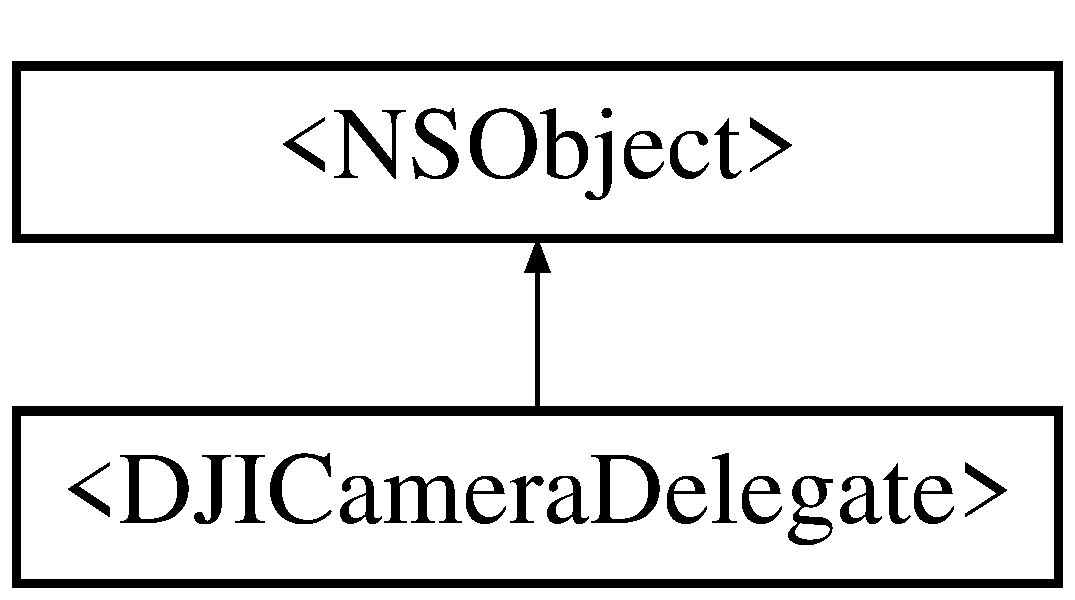
\includegraphics[height=2.000000cm]{protocol_d_j_i_camera_delegate-p}
\end{center}
\end{figure}
\subsection*{Instance Methods}
\begin{DoxyCompactItemize}
\item 
(void) -\/ \hyperlink{protocol_d_j_i_camera_delegate-p_a82dc726780bf9334cf2a0e5c33a45ce2}{camera\+:did\+Received\+Video\+Data\+:length\+:}
\item 
(void) -\/ \hyperlink{protocol_d_j_i_camera_delegate-p_a24b371f3bff14e1eaa922f3ac4a821a9}{camera\+:did\+Update\+System\+State\+:}
\item 
(void) -\/ \hyperlink{protocol_d_j_i_camera_delegate-p_acc6d42ada266a43eb8dbe97198b51694}{camera\+:did\+Generated\+New\+Media\+:}
\end{DoxyCompactItemize}


\subsection{Method Documentation}
\hypertarget{protocol_d_j_i_camera_delegate-p_acc6d42ada266a43eb8dbe97198b51694}{\index{D\+J\+I\+Camera\+Delegate-\/p@{D\+J\+I\+Camera\+Delegate-\/p}!camera\+:did\+Generated\+New\+Media\+:@{camera\+:did\+Generated\+New\+Media\+:}}
\index{camera\+:did\+Generated\+New\+Media\+:@{camera\+:did\+Generated\+New\+Media\+:}!D\+J\+I\+Camera\+Delegate-\/p@{D\+J\+I\+Camera\+Delegate-\/p}}
\subsubsection[{camera\+:did\+Generated\+New\+Media\+:}]{\setlength{\rightskip}{0pt plus 5cm}-\/ (void) camera\+: 
\begin{DoxyParamCaption}
\item[{({\bf D\+J\+I\+Camera} $\ast$)}]{camera}
\item[{didGeneratedNewMedia:({\bf D\+J\+I\+Media} $\ast$)}]{new\+Media}
\end{DoxyParamCaption}
\hspace{0.3cm}{\ttfamily [optional]}}}\label{protocol_d_j_i_camera_delegate-p_acc6d42ada266a43eb8dbe97198b51694}
Push media info while completed take photo or recording.


\begin{DoxyParams}{Parameters}
{\em new\+Media} & The new media object. \\
\hline
\end{DoxyParams}
\hypertarget{protocol_d_j_i_camera_delegate-p_a82dc726780bf9334cf2a0e5c33a45ce2}{\index{D\+J\+I\+Camera\+Delegate-\/p@{D\+J\+I\+Camera\+Delegate-\/p}!camera\+:did\+Received\+Video\+Data\+:length\+:@{camera\+:did\+Received\+Video\+Data\+:length\+:}}
\index{camera\+:did\+Received\+Video\+Data\+:length\+:@{camera\+:did\+Received\+Video\+Data\+:length\+:}!D\+J\+I\+Camera\+Delegate-\/p@{D\+J\+I\+Camera\+Delegate-\/p}}
\subsubsection[{camera\+:did\+Received\+Video\+Data\+:length\+:}]{\setlength{\rightskip}{0pt plus 5cm}-\/ (void) camera\+: 
\begin{DoxyParamCaption}
\item[{({\bf D\+J\+I\+Camera} $\ast$)}]{camera}
\item[{didReceivedVideoData:(uint8\+\_\+t $\ast$)}]{video\+Buffer}
\item[{length:(int)}]{length}
\end{DoxyParamCaption}
\hspace{0.3cm}{\ttfamily [required]}}}\label{protocol_d_j_i_camera_delegate-p_a82dc726780bf9334cf2a0e5c33a45ce2}
Video data interface


\begin{DoxyParams}{Parameters}
{\em video\+Buffer} & H.\+264 video data buffer \\
\hline
{\em length} & H.\+264 video data length \\
\hline
\end{DoxyParams}
\hypertarget{protocol_d_j_i_camera_delegate-p_a24b371f3bff14e1eaa922f3ac4a821a9}{\index{D\+J\+I\+Camera\+Delegate-\/p@{D\+J\+I\+Camera\+Delegate-\/p}!camera\+:did\+Update\+System\+State\+:@{camera\+:did\+Update\+System\+State\+:}}
\index{camera\+:did\+Update\+System\+State\+:@{camera\+:did\+Update\+System\+State\+:}!D\+J\+I\+Camera\+Delegate-\/p@{D\+J\+I\+Camera\+Delegate-\/p}}
\subsubsection[{camera\+:did\+Update\+System\+State\+:}]{\setlength{\rightskip}{0pt plus 5cm}-\/ (void) camera\+: 
\begin{DoxyParamCaption}
\item[{({\bf D\+J\+I\+Camera} $\ast$)}]{camera}
\item[{didUpdateSystemState:(D\+J\+I\+Camera\+System\+State $\ast$)}]{system\+State}
\end{DoxyParamCaption}
\hspace{0.3cm}{\ttfamily [required]}}}\label{protocol_d_j_i_camera_delegate-p_a24b371f3bff14e1eaa922f3ac4a821a9}
Update the camera's system state. User should call the start\+Camera\+System\+State\+Updates interface to begin updating.


\begin{DoxyParams}{Parameters}
{\em system\+State} & The camera's system state. \\
\hline
\end{DoxyParams}


The documentation for this protocol was generated from the following file\+:\begin{DoxyCompactItemize}
\item 
D\+J\+I\+Camera.\+h\end{DoxyCompactItemize}

\hypertarget{interface_d_j_i_camera_s_d_card_info}{\section{D\+J\+I\+Camera\+S\+D\+Card\+Info Class Reference}
\label{interface_d_j_i_camera_s_d_card_info}\index{D\+J\+I\+Camera\+S\+D\+Card\+Info@{D\+J\+I\+Camera\+S\+D\+Card\+Info}}
}


{\ttfamily \#import $<$D\+J\+I\+Camera\+S\+D\+Card\+Info.\+h$>$}

Inheritance diagram for D\+J\+I\+Camera\+S\+D\+Card\+Info\+:\begin{figure}[H]
\begin{center}
\leavevmode
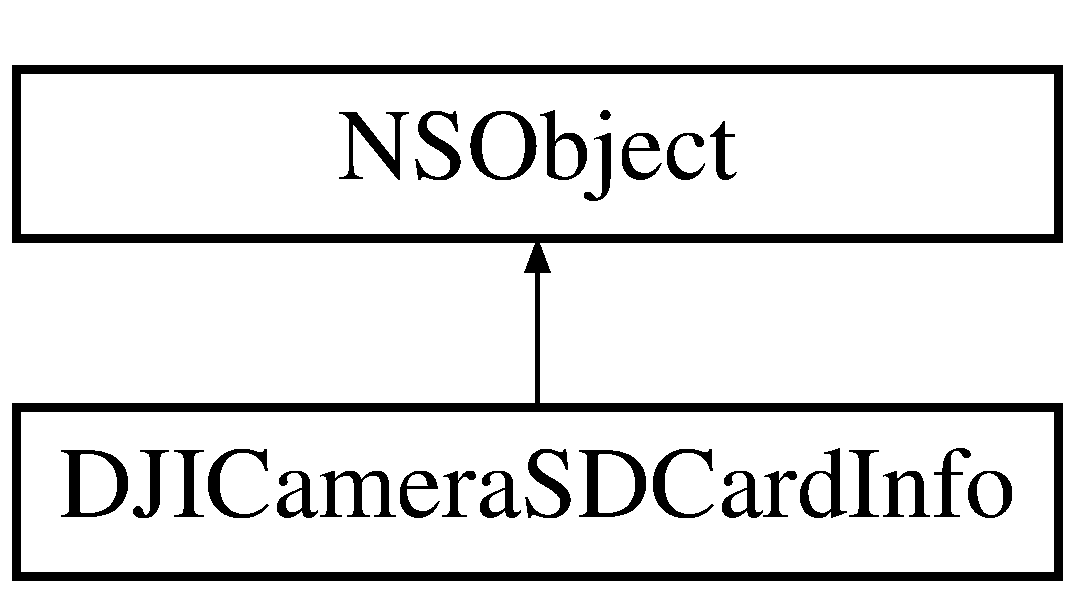
\includegraphics[height=2.000000cm]{interface_d_j_i_camera_s_d_card_info}
\end{center}
\end{figure}
\subsection*{Properties}
\begin{DoxyCompactItemize}
\item 
B\+O\+O\+L \hyperlink{interface_d_j_i_camera_s_d_card_info_a0fb344a71d20c3f43bb4b68c51300cbb}{has\+Error}
\item 
B\+O\+O\+L \hyperlink{interface_d_j_i_camera_s_d_card_info_a3e3d67655f38d71c0aab6ae7a132e396}{read\+Only}
\item 
B\+O\+O\+L \hyperlink{interface_d_j_i_camera_s_d_card_info_af79c37797d1d0eb7e2b132b217a94290}{invalid\+Format}
\item 
B\+O\+O\+L \hyperlink{interface_d_j_i_camera_s_d_card_info_ab8cf4478b6ae1e49c1fe4cb4969b26e5}{is\+Formated}
\item 
B\+O\+O\+L \hyperlink{interface_d_j_i_camera_s_d_card_info_a61802b45c064b527ff835725e16e4c30}{is\+Formating}
\item 
B\+O\+O\+L \hyperlink{interface_d_j_i_camera_s_d_card_info_a4e68054993b2d9bd2d0fc544c6e1f380}{is\+Full}
\item 
B\+O\+O\+L \hyperlink{interface_d_j_i_camera_s_d_card_info_af59a91c8c2d10546da7168d7d10310ed}{is\+Valid}
\item 
B\+O\+O\+L \hyperlink{interface_d_j_i_camera_s_d_card_info_ad625b9a7a4047c03c0419a90b1fa335b}{is\+Inserted}
\item 
int \hyperlink{interface_d_j_i_camera_s_d_card_info_a880e1b513893d27cc94c83e405a72667}{total\+Size}
\item 
int \hyperlink{interface_d_j_i_camera_s_d_card_info_aa44ca2930b598e41704aaa9ba67c95dc}{remain\+Size}
\item 
int \hyperlink{interface_d_j_i_camera_s_d_card_info_a27f92f3e797ec9a590ac62545d8c3d03}{available\+Capture\+Count}
\end{DoxyCompactItemize}


\subsection{Detailed Description}
Provide S\+D card informations and status 

\subsection{Property Documentation}
\hypertarget{interface_d_j_i_camera_s_d_card_info_a27f92f3e797ec9a590ac62545d8c3d03}{\index{D\+J\+I\+Camera\+S\+D\+Card\+Info@{D\+J\+I\+Camera\+S\+D\+Card\+Info}!available\+Capture\+Count@{available\+Capture\+Count}}
\index{available\+Capture\+Count@{available\+Capture\+Count}!D\+J\+I\+Camera\+S\+D\+Card\+Info@{D\+J\+I\+Camera\+S\+D\+Card\+Info}}
\subsubsection[{available\+Capture\+Count}]{\setlength{\rightskip}{0pt plus 5cm}-\/ (int) available\+Capture\+Count\hspace{0.3cm}{\ttfamily [read]}, {\ttfamily [nonatomic]}, {\ttfamily [assign]}}}\label{interface_d_j_i_camera_s_d_card_info_a27f92f3e797ec9a590ac62545d8c3d03}
The available count for taking photo \hypertarget{interface_d_j_i_camera_s_d_card_info_a0fb344a71d20c3f43bb4b68c51300cbb}{\index{D\+J\+I\+Camera\+S\+D\+Card\+Info@{D\+J\+I\+Camera\+S\+D\+Card\+Info}!has\+Error@{has\+Error}}
\index{has\+Error@{has\+Error}!D\+J\+I\+Camera\+S\+D\+Card\+Info@{D\+J\+I\+Camera\+S\+D\+Card\+Info}}
\subsubsection[{has\+Error}]{\setlength{\rightskip}{0pt plus 5cm}-\/ (B\+O\+O\+L) has\+Error\hspace{0.3cm}{\ttfamily [read]}, {\ttfamily [nonatomic]}, {\ttfamily [assign]}}}\label{interface_d_j_i_camera_s_d_card_info_a0fb344a71d20c3f43bb4b68c51300cbb}
Indicate some error occur while access the sd card \hypertarget{interface_d_j_i_camera_s_d_card_info_af79c37797d1d0eb7e2b132b217a94290}{\index{D\+J\+I\+Camera\+S\+D\+Card\+Info@{D\+J\+I\+Camera\+S\+D\+Card\+Info}!invalid\+Format@{invalid\+Format}}
\index{invalid\+Format@{invalid\+Format}!D\+J\+I\+Camera\+S\+D\+Card\+Info@{D\+J\+I\+Camera\+S\+D\+Card\+Info}}
\subsubsection[{invalid\+Format}]{\setlength{\rightskip}{0pt plus 5cm}-\/ (B\+O\+O\+L) invalid\+Format\hspace{0.3cm}{\ttfamily [read]}, {\ttfamily [nonatomic]}, {\ttfamily [assign]}}}\label{interface_d_j_i_camera_s_d_card_info_af79c37797d1d0eb7e2b132b217a94290}
The S\+D card invalid format \hypertarget{interface_d_j_i_camera_s_d_card_info_ab8cf4478b6ae1e49c1fe4cb4969b26e5}{\index{D\+J\+I\+Camera\+S\+D\+Card\+Info@{D\+J\+I\+Camera\+S\+D\+Card\+Info}!is\+Formated@{is\+Formated}}
\index{is\+Formated@{is\+Formated}!D\+J\+I\+Camera\+S\+D\+Card\+Info@{D\+J\+I\+Camera\+S\+D\+Card\+Info}}
\subsubsection[{is\+Formated}]{\setlength{\rightskip}{0pt plus 5cm}-\/ (B\+O\+O\+L) is\+Formated\hspace{0.3cm}{\ttfamily [read]}, {\ttfamily [nonatomic]}, {\ttfamily [assign]}}}\label{interface_d_j_i_camera_s_d_card_info_ab8cf4478b6ae1e49c1fe4cb4969b26e5}
The S\+D card is formated \hypertarget{interface_d_j_i_camera_s_d_card_info_a61802b45c064b527ff835725e16e4c30}{\index{D\+J\+I\+Camera\+S\+D\+Card\+Info@{D\+J\+I\+Camera\+S\+D\+Card\+Info}!is\+Formating@{is\+Formating}}
\index{is\+Formating@{is\+Formating}!D\+J\+I\+Camera\+S\+D\+Card\+Info@{D\+J\+I\+Camera\+S\+D\+Card\+Info}}
\subsubsection[{is\+Formating}]{\setlength{\rightskip}{0pt plus 5cm}-\/ (B\+O\+O\+L) is\+Formating\hspace{0.3cm}{\ttfamily [read]}, {\ttfamily [nonatomic]}, {\ttfamily [assign]}}}\label{interface_d_j_i_camera_s_d_card_info_a61802b45c064b527ff835725e16e4c30}
The S\+D card is formating \hypertarget{interface_d_j_i_camera_s_d_card_info_a4e68054993b2d9bd2d0fc544c6e1f380}{\index{D\+J\+I\+Camera\+S\+D\+Card\+Info@{D\+J\+I\+Camera\+S\+D\+Card\+Info}!is\+Full@{is\+Full}}
\index{is\+Full@{is\+Full}!D\+J\+I\+Camera\+S\+D\+Card\+Info@{D\+J\+I\+Camera\+S\+D\+Card\+Info}}
\subsubsection[{is\+Full}]{\setlength{\rightskip}{0pt plus 5cm}-\/ (B\+O\+O\+L) is\+Full\hspace{0.3cm}{\ttfamily [read]}, {\ttfamily [nonatomic]}, {\ttfamily [assign]}}}\label{interface_d_j_i_camera_s_d_card_info_a4e68054993b2d9bd2d0fc544c6e1f380}
The S\+D card is full \hypertarget{interface_d_j_i_camera_s_d_card_info_ad625b9a7a4047c03c0419a90b1fa335b}{\index{D\+J\+I\+Camera\+S\+D\+Card\+Info@{D\+J\+I\+Camera\+S\+D\+Card\+Info}!is\+Inserted@{is\+Inserted}}
\index{is\+Inserted@{is\+Inserted}!D\+J\+I\+Camera\+S\+D\+Card\+Info@{D\+J\+I\+Camera\+S\+D\+Card\+Info}}
\subsubsection[{is\+Inserted}]{\setlength{\rightskip}{0pt plus 5cm}-\/ (B\+O\+O\+L) is\+Inserted\hspace{0.3cm}{\ttfamily [read]}, {\ttfamily [nonatomic]}, {\ttfamily [assign]}}}\label{interface_d_j_i_camera_s_d_card_info_ad625b9a7a4047c03c0419a90b1fa335b}
Whether the S\+D card is inserted into the camera. \hypertarget{interface_d_j_i_camera_s_d_card_info_af59a91c8c2d10546da7168d7d10310ed}{\index{D\+J\+I\+Camera\+S\+D\+Card\+Info@{D\+J\+I\+Camera\+S\+D\+Card\+Info}!is\+Valid@{is\+Valid}}
\index{is\+Valid@{is\+Valid}!D\+J\+I\+Camera\+S\+D\+Card\+Info@{D\+J\+I\+Camera\+S\+D\+Card\+Info}}
\subsubsection[{is\+Valid}]{\setlength{\rightskip}{0pt plus 5cm}-\/ (B\+O\+O\+L) is\+Valid\hspace{0.3cm}{\ttfamily [read]}, {\ttfamily [nonatomic]}, {\ttfamily [assign]}}}\label{interface_d_j_i_camera_s_d_card_info_af59a91c8c2d10546da7168d7d10310ed}
Whether the S\+D card is a valid card \hypertarget{interface_d_j_i_camera_s_d_card_info_a3e3d67655f38d71c0aab6ae7a132e396}{\index{D\+J\+I\+Camera\+S\+D\+Card\+Info@{D\+J\+I\+Camera\+S\+D\+Card\+Info}!read\+Only@{read\+Only}}
\index{read\+Only@{read\+Only}!D\+J\+I\+Camera\+S\+D\+Card\+Info@{D\+J\+I\+Camera\+S\+D\+Card\+Info}}
\subsubsection[{read\+Only}]{\setlength{\rightskip}{0pt plus 5cm}-\/ (B\+O\+O\+L) read\+Only\hspace{0.3cm}{\ttfamily [read]}, {\ttfamily [nonatomic]}, {\ttfamily [assign]}}}\label{interface_d_j_i_camera_s_d_card_info_a3e3d67655f38d71c0aab6ae7a132e396}
The S\+D card is read only \hypertarget{interface_d_j_i_camera_s_d_card_info_aa44ca2930b598e41704aaa9ba67c95dc}{\index{D\+J\+I\+Camera\+S\+D\+Card\+Info@{D\+J\+I\+Camera\+S\+D\+Card\+Info}!remain\+Size@{remain\+Size}}
\index{remain\+Size@{remain\+Size}!D\+J\+I\+Camera\+S\+D\+Card\+Info@{D\+J\+I\+Camera\+S\+D\+Card\+Info}}
\subsubsection[{remain\+Size}]{\setlength{\rightskip}{0pt plus 5cm}-\/ (int) remain\+Size\hspace{0.3cm}{\ttfamily [read]}, {\ttfamily [nonatomic]}, {\ttfamily [assign]}}}\label{interface_d_j_i_camera_s_d_card_info_aa44ca2930b598e41704aaa9ba67c95dc}
Remain size of the S\+D card \hypertarget{interface_d_j_i_camera_s_d_card_info_a880e1b513893d27cc94c83e405a72667}{\index{D\+J\+I\+Camera\+S\+D\+Card\+Info@{D\+J\+I\+Camera\+S\+D\+Card\+Info}!total\+Size@{total\+Size}}
\index{total\+Size@{total\+Size}!D\+J\+I\+Camera\+S\+D\+Card\+Info@{D\+J\+I\+Camera\+S\+D\+Card\+Info}}
\subsubsection[{total\+Size}]{\setlength{\rightskip}{0pt plus 5cm}-\/ (int) total\+Size\hspace{0.3cm}{\ttfamily [read]}, {\ttfamily [nonatomic]}, {\ttfamily [assign]}}}\label{interface_d_j_i_camera_s_d_card_info_a880e1b513893d27cc94c83e405a72667}
Total size of the S\+D card. 

The documentation for this class was generated from the following file\+:\begin{DoxyCompactItemize}
\item 
D\+J\+I\+Camera\+S\+D\+Card\+Info.\+h\end{DoxyCompactItemize}

\hypertarget{interface_d_j_i_drone}{\section{D\+J\+I\+Drone Class Reference}
\label{interface_d_j_i_drone}\index{D\+J\+I\+Drone@{D\+J\+I\+Drone}}
}
Inheritance diagram for D\+J\+I\+Drone\+:\begin{figure}[H]
\begin{center}
\leavevmode
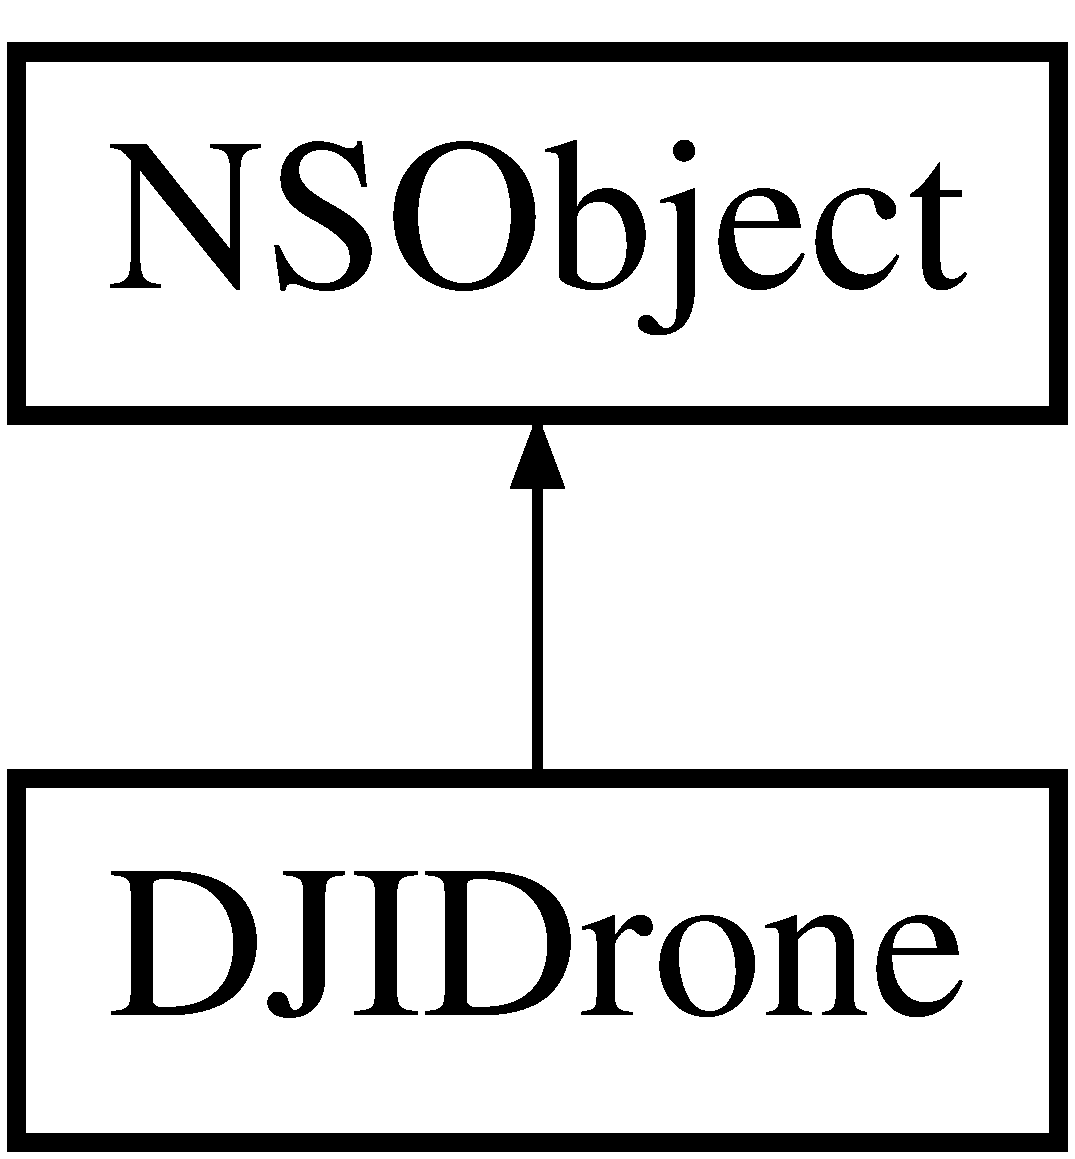
\includegraphics[height=2.000000cm]{interface_d_j_i_drone}
\end{center}
\end{figure}
\subsection*{Instance Methods}
\begin{DoxyCompactItemize}
\item 
(id) -\/ \hyperlink{interface_d_j_i_drone_ad6afee4fa10687223ffdfabb3a96cc76}{init\+With\+Type\+:}
\item 
(void) -\/ \hyperlink{interface_d_j_i_drone_a7f2da8feee3a5a339140856402786e4c}{connect\+To\+Drone}
\item 
(void) -\/ \hyperlink{interface_d_j_i_drone_acf84bad64f001cda75b6fec209e6d504}{disconnect\+To\+Drone}
\item 
(void) -\/ \hyperlink{interface_d_j_i_drone_aa1b8f8b9c4bb3dffb49979285f578696}{destroy}
\end{DoxyCompactItemize}
\subsection*{Protected Attributes}
\begin{DoxyCompactItemize}
\item 
\hypertarget{interface_d_j_i_drone_a12680c7d92b2f6ce84934db2795d0dc2}{D\+J\+I\+Drone\+Type {\bfseries \+\_\+drone\+Type}}\label{interface_d_j_i_drone_a12680c7d92b2f6ce84934db2795d0dc2}

\end{DoxyCompactItemize}
\subsection*{Properties}
\begin{DoxyCompactItemize}
\item 
id$<$ D\+J\+I\+Drone\+Delegate $>$ \hyperlink{interface_d_j_i_drone_a348f8faf9da7670e19289130c4490c9a}{delegate}
\item 
D\+J\+I\+Drone\+Type \hyperlink{interface_d_j_i_drone_a5f830dba99822f494acfd499308d3818}{drone\+Type}
\item 
\hyperlink{interface_d_j_i_camera}{D\+J\+I\+Camera} $\ast$ \hyperlink{interface_d_j_i_drone_adf9479847eb1e9826dcadfeeab3b12d0}{camera}
\item 
\hyperlink{interface_d_j_i_main_controller}{D\+J\+I\+Main\+Controller} $\ast$ \hyperlink{interface_d_j_i_drone_a7f05dfcf7d06e7663926954211683eb4}{main\+Controller}
\item 
\hyperlink{interface_d_j_i_gimbal}{D\+J\+I\+Gimbal} $\ast$ \hyperlink{interface_d_j_i_drone_a4e03ec9b32a2ab6a9755ff9c065cca76}{gimbal}
\item 
\hyperlink{interface_d_j_i_range_extender}{D\+J\+I\+Range\+Extender} $\ast$ \hyperlink{interface_d_j_i_drone_aad1a0914357ef128bb16d52f8a7670e4}{range\+Extender}
\item 
\hyperlink{interface_d_j_i_battery}{D\+J\+I\+Battery} $\ast$ \hyperlink{interface_d_j_i_drone_a762451fe8b64cbbc3c9d288ef29b0f99}{smart\+Battery}
\end{DoxyCompactItemize}


\subsection{Method Documentation}
\hypertarget{interface_d_j_i_drone_a7f2da8feee3a5a339140856402786e4c}{\index{D\+J\+I\+Drone@{D\+J\+I\+Drone}!connect\+To\+Drone@{connect\+To\+Drone}}
\index{connect\+To\+Drone@{connect\+To\+Drone}!D\+J\+I\+Drone@{D\+J\+I\+Drone}}
\subsubsection[{connect\+To\+Drone}]{\setlength{\rightskip}{0pt plus 5cm}-\/ (void) connect\+To\+Drone 
\begin{DoxyParamCaption}
{}
\end{DoxyParamCaption}
}}\label{interface_d_j_i_drone_a7f2da8feee3a5a339140856402786e4c}
Connect to the drone. once this function was called, the \hyperlink{interface_d_j_i_drone}{D\+J\+I\+Drone} will automatically connect to the drone \hypertarget{interface_d_j_i_drone_aa1b8f8b9c4bb3dffb49979285f578696}{\index{D\+J\+I\+Drone@{D\+J\+I\+Drone}!destroy@{destroy}}
\index{destroy@{destroy}!D\+J\+I\+Drone@{D\+J\+I\+Drone}}
\subsubsection[{destroy}]{\setlength{\rightskip}{0pt plus 5cm}-\/ (void) destroy 
\begin{DoxyParamCaption}
{}
\end{DoxyParamCaption}
}}\label{interface_d_j_i_drone_aa1b8f8b9c4bb3dffb49979285f578696}
Destroy the drone object, user should call this interface to release all objects. \hypertarget{interface_d_j_i_drone_acf84bad64f001cda75b6fec209e6d504}{\index{D\+J\+I\+Drone@{D\+J\+I\+Drone}!disconnect\+To\+Drone@{disconnect\+To\+Drone}}
\index{disconnect\+To\+Drone@{disconnect\+To\+Drone}!D\+J\+I\+Drone@{D\+J\+I\+Drone}}
\subsubsection[{disconnect\+To\+Drone}]{\setlength{\rightskip}{0pt plus 5cm}-\/ (void) disconnect\+To\+Drone 
\begin{DoxyParamCaption}
{}
\end{DoxyParamCaption}
}}\label{interface_d_j_i_drone_acf84bad64f001cda75b6fec209e6d504}
Disconnect to the drone. \hypertarget{interface_d_j_i_drone_ad6afee4fa10687223ffdfabb3a96cc76}{\index{D\+J\+I\+Drone@{D\+J\+I\+Drone}!init\+With\+Type\+:@{init\+With\+Type\+:}}
\index{init\+With\+Type\+:@{init\+With\+Type\+:}!D\+J\+I\+Drone@{D\+J\+I\+Drone}}
\subsubsection[{init\+With\+Type\+:}]{\setlength{\rightskip}{0pt plus 5cm}-\/ (id) init\+With\+Type\+: 
\begin{DoxyParamCaption}
\item[{(D\+J\+I\+Drone\+Type)}]{type}
\end{DoxyParamCaption}
}}\label{interface_d_j_i_drone_ad6afee4fa10687223ffdfabb3a96cc76}
init drone object with type 

\subsection{Property Documentation}
\hypertarget{interface_d_j_i_drone_adf9479847eb1e9826dcadfeeab3b12d0}{\index{D\+J\+I\+Drone@{D\+J\+I\+Drone}!camera@{camera}}
\index{camera@{camera}!D\+J\+I\+Drone@{D\+J\+I\+Drone}}
\subsubsection[{camera}]{\setlength{\rightskip}{0pt plus 5cm}-\/ ({\bf D\+J\+I\+Camera}$\ast$) camera\hspace{0.3cm}{\ttfamily [read]}, {\ttfamily [nonatomic]}, {\ttfamily [assign]}}}\label{interface_d_j_i_drone_adf9479847eb1e9826dcadfeeab3b12d0}
Drone's camera. \hypertarget{interface_d_j_i_drone_a348f8faf9da7670e19289130c4490c9a}{\index{D\+J\+I\+Drone@{D\+J\+I\+Drone}!delegate@{delegate}}
\index{delegate@{delegate}!D\+J\+I\+Drone@{D\+J\+I\+Drone}}
\subsubsection[{delegate}]{\setlength{\rightskip}{0pt plus 5cm}-\/ (id$<$D\+J\+I\+Drone\+Delegate$>$) delegate\hspace{0.3cm}{\ttfamily [read]}, {\ttfamily [write]}, {\ttfamily [nonatomic]}, {\ttfamily [weak]}}}\label{interface_d_j_i_drone_a348f8faf9da7670e19289130c4490c9a}
Drone delegate \hypertarget{interface_d_j_i_drone_a5f830dba99822f494acfd499308d3818}{\index{D\+J\+I\+Drone@{D\+J\+I\+Drone}!drone\+Type@{drone\+Type}}
\index{drone\+Type@{drone\+Type}!D\+J\+I\+Drone@{D\+J\+I\+Drone}}
\subsubsection[{drone\+Type}]{\setlength{\rightskip}{0pt plus 5cm}-\/ (D\+J\+I\+Drone\+Type) drone\+Type\hspace{0.3cm}{\ttfamily [read]}, {\ttfamily [nonatomic]}, {\ttfamily [assign]}}}\label{interface_d_j_i_drone_a5f830dba99822f494acfd499308d3818}
Drone type \hypertarget{interface_d_j_i_drone_a4e03ec9b32a2ab6a9755ff9c065cca76}{\index{D\+J\+I\+Drone@{D\+J\+I\+Drone}!gimbal@{gimbal}}
\index{gimbal@{gimbal}!D\+J\+I\+Drone@{D\+J\+I\+Drone}}
\subsubsection[{gimbal}]{\setlength{\rightskip}{0pt plus 5cm}-\/ ({\bf D\+J\+I\+Gimbal}$\ast$) gimbal\hspace{0.3cm}{\ttfamily [read]}, {\ttfamily [nonatomic]}, {\ttfamily [assign]}}}\label{interface_d_j_i_drone_a4e03ec9b32a2ab6a9755ff9c065cca76}
Drones' gimbal. \hypertarget{interface_d_j_i_drone_a7f05dfcf7d06e7663926954211683eb4}{\index{D\+J\+I\+Drone@{D\+J\+I\+Drone}!main\+Controller@{main\+Controller}}
\index{main\+Controller@{main\+Controller}!D\+J\+I\+Drone@{D\+J\+I\+Drone}}
\subsubsection[{main\+Controller}]{\setlength{\rightskip}{0pt plus 5cm}-\/ ({\bf D\+J\+I\+Main\+Controller}$\ast$) main\+Controller\hspace{0.3cm}{\ttfamily [read]}, {\ttfamily [nonatomic]}, {\ttfamily [assign]}}}\label{interface_d_j_i_drone_a7f05dfcf7d06e7663926954211683eb4}
Drone's main controller. \hypertarget{interface_d_j_i_drone_aad1a0914357ef128bb16d52f8a7670e4}{\index{D\+J\+I\+Drone@{D\+J\+I\+Drone}!range\+Extender@{range\+Extender}}
\index{range\+Extender@{range\+Extender}!D\+J\+I\+Drone@{D\+J\+I\+Drone}}
\subsubsection[{range\+Extender}]{\setlength{\rightskip}{0pt plus 5cm}-\/ ({\bf D\+J\+I\+Range\+Extender}$\ast$) range\+Extender\hspace{0.3cm}{\ttfamily [read]}, {\ttfamily [nonatomic]}, {\ttfamily [assign]}}}\label{interface_d_j_i_drone_aad1a0914357ef128bb16d52f8a7670e4}
Range extender. \hypertarget{interface_d_j_i_drone_a762451fe8b64cbbc3c9d288ef29b0f99}{\index{D\+J\+I\+Drone@{D\+J\+I\+Drone}!smart\+Battery@{smart\+Battery}}
\index{smart\+Battery@{smart\+Battery}!D\+J\+I\+Drone@{D\+J\+I\+Drone}}
\subsubsection[{smart\+Battery}]{\setlength{\rightskip}{0pt plus 5cm}-\/ ({\bf D\+J\+I\+Battery}$\ast$) smart\+Battery\hspace{0.3cm}{\ttfamily [read]}, {\ttfamily [nonatomic]}, {\ttfamily [assign]}}}\label{interface_d_j_i_drone_a762451fe8b64cbbc3c9d288ef29b0f99}
Smart battery 

The documentation for this class was generated from the following file\+:\begin{DoxyCompactItemize}
\item 
D\+J\+I\+Drone.\+h\end{DoxyCompactItemize}

\hypertarget{interface_d_j_i_error}{\section{D\+J\+I\+Error Class Reference}
\label{interface_d_j_i_error}\index{D\+J\+I\+Error@{D\+J\+I\+Error}}
}
Inheritance diagram for D\+J\+I\+Error\+:\begin{figure}[H]
\begin{center}
\leavevmode
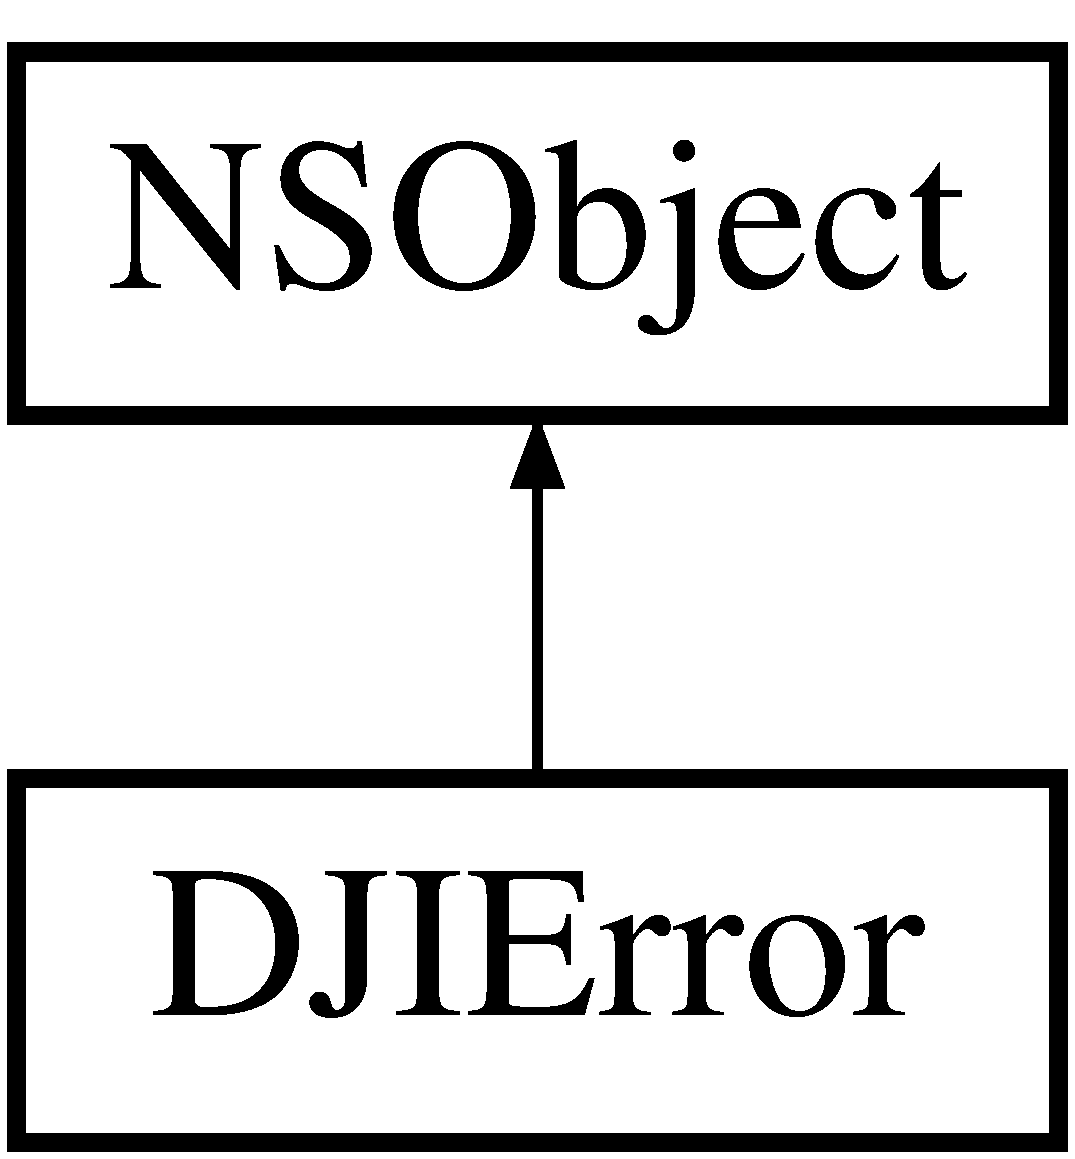
\includegraphics[height=2.000000cm]{interface_d_j_i_error}
\end{center}
\end{figure}
\subsection*{Instance Methods}
\begin{DoxyCompactItemize}
\item 
\hypertarget{interface_d_j_i_error_af4ede61e5a89677364d5225d88880c4a}{(id) -\/ {\bfseries init\+With\+Error\+Code\+:}}\label{interface_d_j_i_error_af4ede61e5a89677364d5225d88880c4a}

\end{DoxyCompactItemize}
\subsection*{Properties}
\begin{DoxyCompactItemize}
\item 
int \hyperlink{interface_d_j_i_error_a92c9fa51ec6acea8d7dad2dd46346372}{error\+Code}
\item 
N\+S\+String $\ast$ \hyperlink{interface_d_j_i_error_a6f210d906aad9322560db1abec9e2e51}{error\+Description}
\end{DoxyCompactItemize}


\subsection{Property Documentation}
\hypertarget{interface_d_j_i_error_a92c9fa51ec6acea8d7dad2dd46346372}{\index{D\+J\+I\+Error@{D\+J\+I\+Error}!error\+Code@{error\+Code}}
\index{error\+Code@{error\+Code}!D\+J\+I\+Error@{D\+J\+I\+Error}}
\subsubsection[{error\+Code}]{\setlength{\rightskip}{0pt plus 5cm}-\/ (int) error\+Code\hspace{0.3cm}{\ttfamily [read]}, {\ttfamily [nonatomic]}, {\ttfamily [assign]}}}\label{interface_d_j_i_error_a92c9fa51ec6acea8d7dad2dd46346372}
Error code. defned as \char`\"{}\+E\+R\+R\+\_\+xxx\char`\"{} \hypertarget{interface_d_j_i_error_a6f210d906aad9322560db1abec9e2e51}{\index{D\+J\+I\+Error@{D\+J\+I\+Error}!error\+Description@{error\+Description}}
\index{error\+Description@{error\+Description}!D\+J\+I\+Error@{D\+J\+I\+Error}}
\subsubsection[{error\+Description}]{\setlength{\rightskip}{0pt plus 5cm}-\/ (N\+S\+String$\ast$) error\+Description\hspace{0.3cm}{\ttfamily [read]}, {\ttfamily [nonatomic]}, {\ttfamily [assign]}}}\label{interface_d_j_i_error_a6f210d906aad9322560db1abec9e2e51}
Error descritpion. 

The documentation for this class was generated from the following file\+:\begin{DoxyCompactItemize}
\item 
D\+J\+I\+Error.\+h\end{DoxyCompactItemize}

\hypertarget{interface_d_j_i_gimbal}{\section{D\+J\+I\+Gimbal Class Reference}
\label{interface_d_j_i_gimbal}\index{D\+J\+I\+Gimbal@{D\+J\+I\+Gimbal}}
}
Inheritance diagram for D\+J\+I\+Gimbal\+:\begin{figure}[H]
\begin{center}
\leavevmode
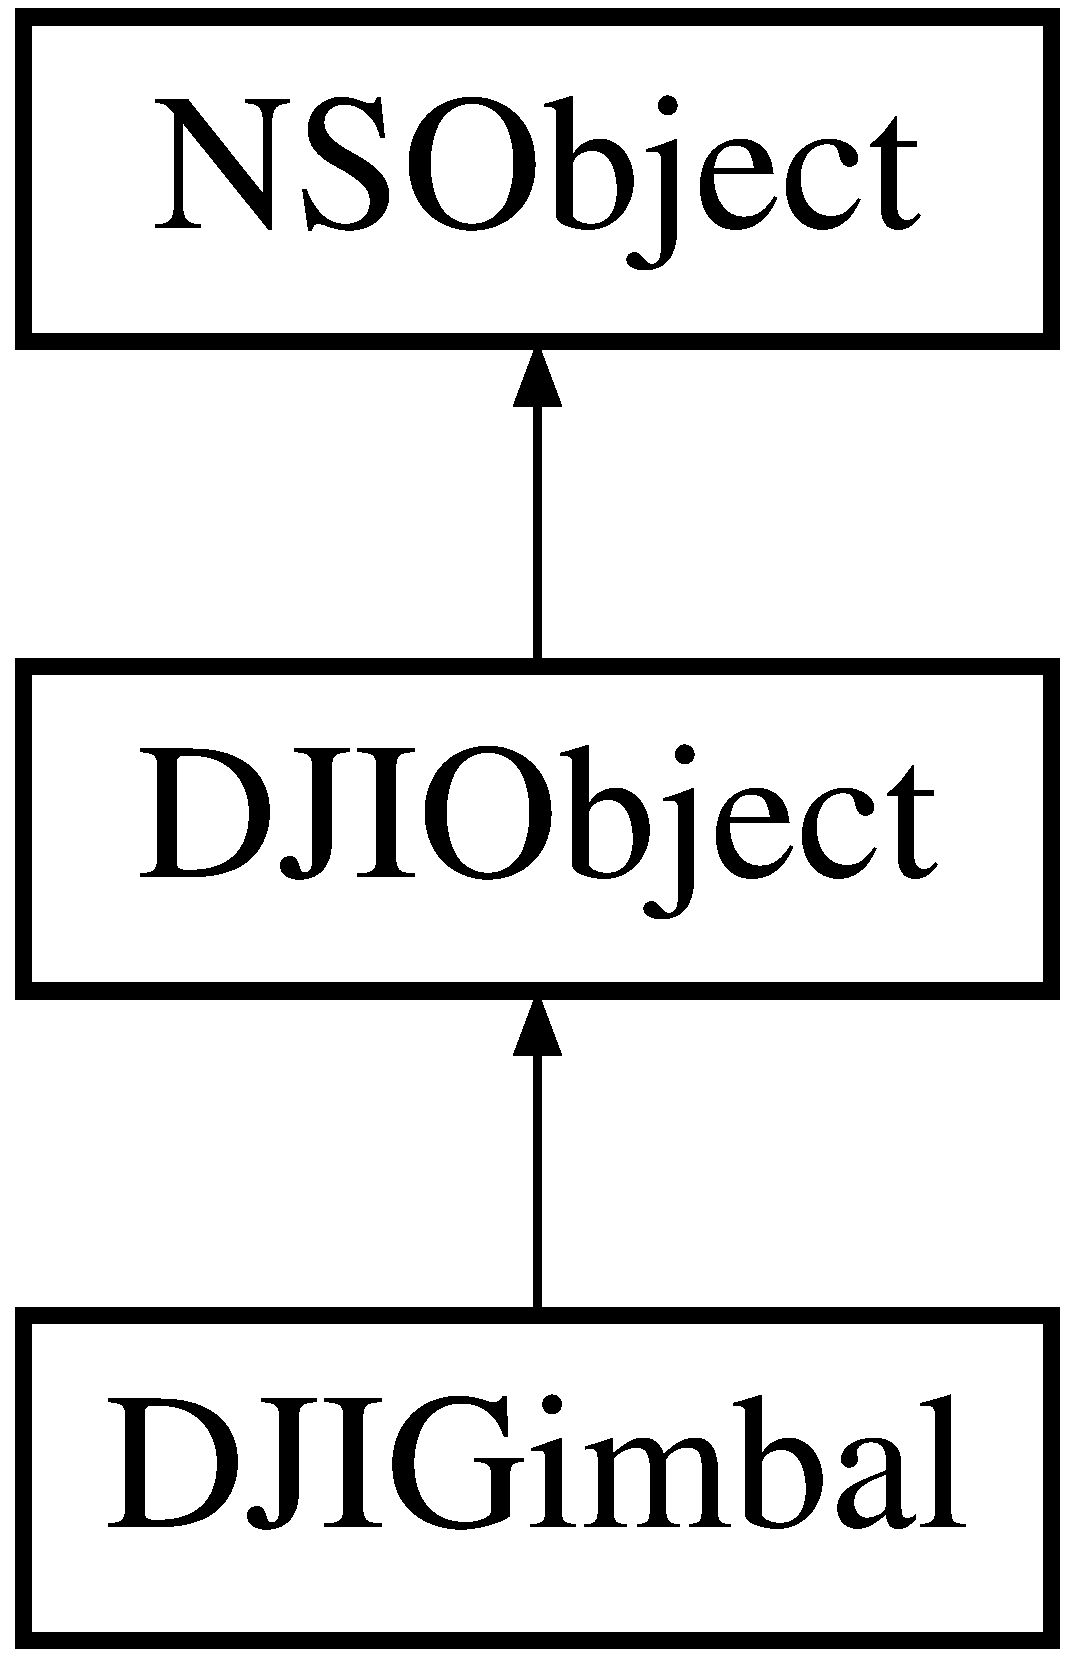
\includegraphics[height=3.000000cm]{interface_d_j_i_gimbal}
\end{center}
\end{figure}
\subsection*{Instance Methods}
\begin{DoxyCompactItemize}
\item 
(\hyperlink{interface_d_j_i_gimbal_capacity}{D\+J\+I\+Gimbal\+Capacity} $\ast$) -\/ \hyperlink{interface_d_j_i_gimbal_a38243bb650051f5529d0593a4a2fd6eb}{get\+Gimbal\+Capacity}
\item 
\hypertarget{interface_d_j_i_gimbal_addb61e4458e9f7532c1d7632e3256de8}{(void) -\/ {\bfseries start\+Gimbal\+Attitude\+Updates}}\label{interface_d_j_i_gimbal_addb61e4458e9f7532c1d7632e3256de8}

\item 
\hypertarget{interface_d_j_i_gimbal_ac787980c21cad6ef13094da82d08bcb3}{(void) -\/ {\bfseries stop\+Gimbal\+Attitude\+Updates}}\label{interface_d_j_i_gimbal_ac787980c21cad6ef13094da82d08bcb3}

\item 
\hypertarget{interface_d_j_i_gimbal_abd6ec35ba4e94a188d47bd6f40213837}{(void) -\/ {\bfseries start\+Gimbal\+Attitude\+Update\+To\+Queue\+:with\+Result\+Block\+:}}\label{interface_d_j_i_gimbal_abd6ec35ba4e94a188d47bd6f40213837}

\item 
(void) -\/ \hyperlink{interface_d_j_i_gimbal_a634e261178cf26f486ca4bb9e3fcc5b9}{set\+Gimbal\+Fpv\+Mode\+:with\+Result\+:}
\item 
(void) -\/ \hyperlink{interface_d_j_i_gimbal_ad420acf7e90595bce5504cc02dedeb01}{set\+Gimbal\+Pitch\+:\+Roll\+:\+Yaw\+:with\+Result\+:}
\end{DoxyCompactItemize}
\subsection*{Properties}
\begin{DoxyCompactItemize}
\item 
\hypertarget{interface_d_j_i_gimbal_a3c2df069500e129bb6a9349649d7aa63}{id$<$ \hyperlink{protocol_d_j_i_gimbal_delegate-p}{D\+J\+I\+Gimbal\+Delegate} $>$ {\bfseries delegate}}\label{interface_d_j_i_gimbal_a3c2df069500e129bb6a9349649d7aa63}

\item 
int \hyperlink{interface_d_j_i_gimbal_a3211c1147e24fbb20d09938b2a19dabb}{attitude\+Update\+Interval}
\item 
\hypertarget{interface_d_j_i_gimbal_ad3b500240c4b2a4db0e33fa50040a85c}{\hyperlink{struct_d_j_i_gimbal_attitude}{D\+J\+I\+Gimbal\+Attitude} {\bfseries gimbal\+Attitude}}\label{interface_d_j_i_gimbal_ad3b500240c4b2a4db0e33fa50040a85c}

\end{DoxyCompactItemize}


\subsection{Method Documentation}
\hypertarget{interface_d_j_i_gimbal_a38243bb650051f5529d0593a4a2fd6eb}{\index{D\+J\+I\+Gimbal@{D\+J\+I\+Gimbal}!get\+Gimbal\+Capacity@{get\+Gimbal\+Capacity}}
\index{get\+Gimbal\+Capacity@{get\+Gimbal\+Capacity}!D\+J\+I\+Gimbal@{D\+J\+I\+Gimbal}}
\subsubsection[{get\+Gimbal\+Capacity}]{\setlength{\rightskip}{0pt plus 5cm}-\/ ({\bf D\+J\+I\+Gimbal\+Capacity}$\ast$) get\+Gimbal\+Capacity 
\begin{DoxyParamCaption}
{}
\end{DoxyParamCaption}
}}\label{interface_d_j_i_gimbal_a38243bb650051f5529d0593a4a2fd6eb}
Get the gimbal's capacity.

\begin{DoxyReturn}{Returns}
gimbal capacity, return nil if connection failured. 
\end{DoxyReturn}
\hypertarget{interface_d_j_i_gimbal_a634e261178cf26f486ca4bb9e3fcc5b9}{\index{D\+J\+I\+Gimbal@{D\+J\+I\+Gimbal}!set\+Gimbal\+Fpv\+Mode\+:with\+Result\+:@{set\+Gimbal\+Fpv\+Mode\+:with\+Result\+:}}
\index{set\+Gimbal\+Fpv\+Mode\+:with\+Result\+:@{set\+Gimbal\+Fpv\+Mode\+:with\+Result\+:}!D\+J\+I\+Gimbal@{D\+J\+I\+Gimbal}}
\subsubsection[{set\+Gimbal\+Fpv\+Mode\+:with\+Result\+:}]{\setlength{\rightskip}{0pt plus 5cm}-\/ (void) set\+Gimbal\+Fpv\+Mode\+: 
\begin{DoxyParamCaption}
\item[{(B\+O\+O\+L)}]{is\+Fpv}
\item[{withResult:(D\+J\+I\+Execute\+Result\+Block)}]{block}
\end{DoxyParamCaption}
}}\label{interface_d_j_i_gimbal_a634e261178cf26f486ca4bb9e3fcc5b9}
Set F\+P\+V mode. Typedef of block to be invoked when fpv mode is set success. \hypertarget{interface_d_j_i_gimbal_ad420acf7e90595bce5504cc02dedeb01}{\index{D\+J\+I\+Gimbal@{D\+J\+I\+Gimbal}!set\+Gimbal\+Pitch\+:\+Roll\+:\+Yaw\+:with\+Result\+:@{set\+Gimbal\+Pitch\+:\+Roll\+:\+Yaw\+:with\+Result\+:}}
\index{set\+Gimbal\+Pitch\+:\+Roll\+:\+Yaw\+:with\+Result\+:@{set\+Gimbal\+Pitch\+:\+Roll\+:\+Yaw\+:with\+Result\+:}!D\+J\+I\+Gimbal@{D\+J\+I\+Gimbal}}
\subsubsection[{set\+Gimbal\+Pitch\+:\+Roll\+:\+Yaw\+:with\+Result\+:}]{\setlength{\rightskip}{0pt plus 5cm}-\/ (void) set\+Gimbal\+Pitch\+: 
\begin{DoxyParamCaption}
\item[{({\bf D\+J\+I\+Gimbal\+Rotation})}]{pitch}
\item[{Roll:({\bf D\+J\+I\+Gimbal\+Rotation})}]{roll}
\item[{Yaw:({\bf D\+J\+I\+Gimbal\+Rotation})}]{yaw}
\item[{withResult:(D\+J\+I\+Execute\+Result\+Block)}]{block}
\end{DoxyParamCaption}
}}\label{interface_d_j_i_gimbal_ad420acf7e90595bce5504cc02dedeb01}
Set gimbal's pitch roll yaw rotation.


\begin{DoxyParams}{Parameters}
{\em pitch} & Gimbal's pitch rotation parameter \\
\hline
{\em roll} & Gimbal's roll rotation parameter \\
\hline
{\em yaw} & Gimbal's yaw rotation parameter \\
\hline
\end{DoxyParams}


\subsection{Property Documentation}
\hypertarget{interface_d_j_i_gimbal_a3211c1147e24fbb20d09938b2a19dabb}{\index{D\+J\+I\+Gimbal@{D\+J\+I\+Gimbal}!attitude\+Update\+Interval@{attitude\+Update\+Interval}}
\index{attitude\+Update\+Interval@{attitude\+Update\+Interval}!D\+J\+I\+Gimbal@{D\+J\+I\+Gimbal}}
\subsubsection[{attitude\+Update\+Interval}]{\setlength{\rightskip}{0pt plus 5cm}-\/ (int) attitude\+Update\+Interval\hspace{0.3cm}{\ttfamily [read]}, {\ttfamily [write]}, {\ttfamily [nonatomic]}, {\ttfamily [assign]}}}\label{interface_d_j_i_gimbal_a3211c1147e24fbb20d09938b2a19dabb}
the attitude update time interval, the value should not smaller then 25ms. default is 50ms 

The documentation for this class was generated from the following file\+:\begin{DoxyCompactItemize}
\item 
D\+J\+I\+Gimbal.\+h\end{DoxyCompactItemize}

\hypertarget{struct_d_j_i_gimbal_attitude}{\section{D\+J\+I\+Gimbal\+Attitude Struct Reference}
\label{struct_d_j_i_gimbal_attitude}\index{D\+J\+I\+Gimbal\+Attitude@{D\+J\+I\+Gimbal\+Attitude}}
}
\subsection*{Protected Attributes}
\begin{DoxyCompactItemize}
\item 
\hypertarget{struct_d_j_i_gimbal_attitude_a22b3fa6e0ba757c1b9722e79a27e345f}{int {\bfseries pitch}}\label{struct_d_j_i_gimbal_attitude_a22b3fa6e0ba757c1b9722e79a27e345f}

\item 
\hypertarget{struct_d_j_i_gimbal_attitude_a3544ad6051f8e52a628c35909c8f76ba}{int {\bfseries roll}}\label{struct_d_j_i_gimbal_attitude_a3544ad6051f8e52a628c35909c8f76ba}

\item 
\hypertarget{struct_d_j_i_gimbal_attitude_a6c11f905229dbc99f098d6f3310a5cb0}{int {\bfseries yaw}}\label{struct_d_j_i_gimbal_attitude_a6c11f905229dbc99f098d6f3310a5cb0}

\end{DoxyCompactItemize}


The documentation for this struct was generated from the following file\+:\begin{DoxyCompactItemize}
\item 
D\+J\+I\+Gimbal.\+h\end{DoxyCompactItemize}

\hypertarget{interface_d_j_i_gimbal_capacity}{\section{D\+J\+I\+Gimbal\+Capacity Class Reference}
\label{interface_d_j_i_gimbal_capacity}\index{D\+J\+I\+Gimbal\+Capacity@{D\+J\+I\+Gimbal\+Capacity}}
}
Inheritance diagram for D\+J\+I\+Gimbal\+Capacity\+:\begin{figure}[H]
\begin{center}
\leavevmode
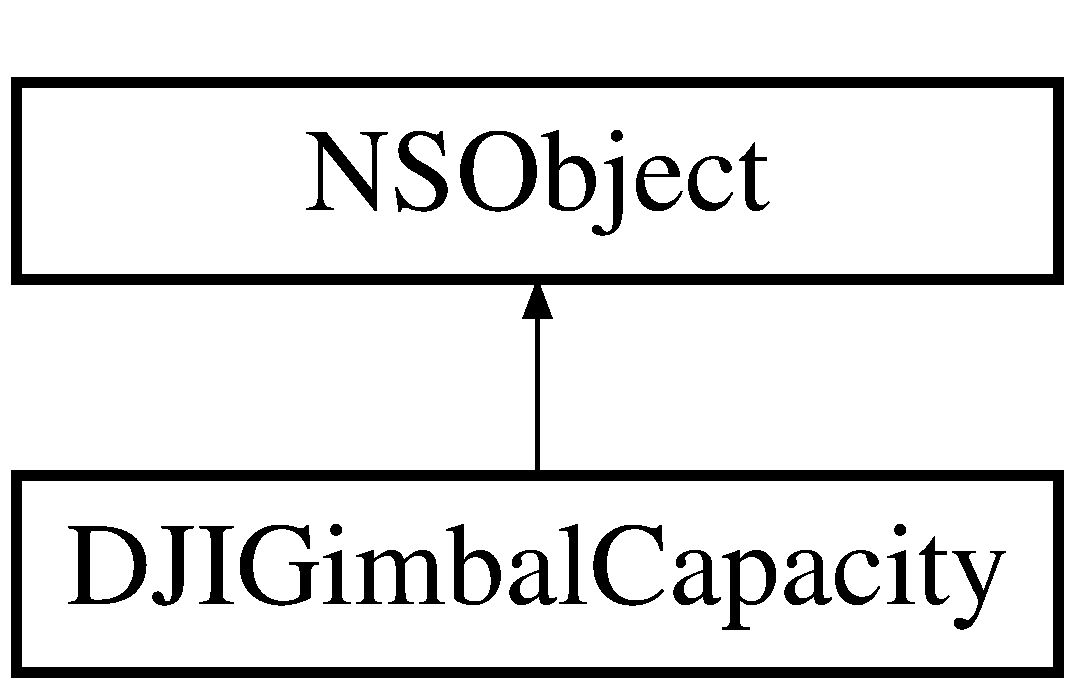
\includegraphics[height=2.000000cm]{interface_d_j_i_gimbal_capacity}
\end{center}
\end{figure}
\subsection*{Properties}
\begin{DoxyCompactItemize}
\item 
B\+O\+O\+L \hyperlink{interface_d_j_i_gimbal_capacity_a353e83a44ff9403020c491b9c06052d6}{pitch\+Available}
\item 
B\+O\+O\+L \hyperlink{interface_d_j_i_gimbal_capacity_a6cd2e6ea9363c2ac0c7de4b067c68fc4}{roll\+Available}
\item 
B\+O\+O\+L \hyperlink{interface_d_j_i_gimbal_capacity_ae1d242caa56f79093279e681fafdf6f9}{yaw\+Available}
\item 
float \hyperlink{interface_d_j_i_gimbal_capacity_a07e3937a56f12c4e55822c75911c4c2f}{max\+Pitch\+Rotation\+Angle}
\item 
float \hyperlink{interface_d_j_i_gimbal_capacity_a8ee53a3ec911e899ddc0c69405b1542f}{min\+Pitch\+Rotation\+Angle}
\item 
float \hyperlink{interface_d_j_i_gimbal_capacity_a75040347b6664f49628ff7c3e33c289c}{max\+Roll\+Rotation\+Angle}
\item 
float \hyperlink{interface_d_j_i_gimbal_capacity_ad153dcc3a5d845ba539a237dd3edba49}{min\+Roll\+Rotation\+Angle}
\item 
float \hyperlink{interface_d_j_i_gimbal_capacity_a88cce121c6e0758ce79f35c0763fdb9a}{max\+Yaw\+Rotation\+Angle}
\item 
float \hyperlink{interface_d_j_i_gimbal_capacity_a1f8386aeb590b5f4010691380a9da02b}{min\+Yaw\+Rotation\+Angle}
\end{DoxyCompactItemize}


\subsection{Property Documentation}
\hypertarget{interface_d_j_i_gimbal_capacity_a07e3937a56f12c4e55822c75911c4c2f}{\index{D\+J\+I\+Gimbal\+Capacity@{D\+J\+I\+Gimbal\+Capacity}!max\+Pitch\+Rotation\+Angle@{max\+Pitch\+Rotation\+Angle}}
\index{max\+Pitch\+Rotation\+Angle@{max\+Pitch\+Rotation\+Angle}!D\+J\+I\+Gimbal\+Capacity@{D\+J\+I\+Gimbal\+Capacity}}
\subsubsection[{max\+Pitch\+Rotation\+Angle}]{\setlength{\rightskip}{0pt plus 5cm}-\/ (float) max\+Pitch\+Rotation\+Angle\hspace{0.3cm}{\ttfamily [read]}, {\ttfamily [write]}, {\ttfamily [nonatomic]}, {\ttfamily [assign]}}}\label{interface_d_j_i_gimbal_capacity_a07e3937a56f12c4e55822c75911c4c2f}
Max controlled angle of pitch \hypertarget{interface_d_j_i_gimbal_capacity_a75040347b6664f49628ff7c3e33c289c}{\index{D\+J\+I\+Gimbal\+Capacity@{D\+J\+I\+Gimbal\+Capacity}!max\+Roll\+Rotation\+Angle@{max\+Roll\+Rotation\+Angle}}
\index{max\+Roll\+Rotation\+Angle@{max\+Roll\+Rotation\+Angle}!D\+J\+I\+Gimbal\+Capacity@{D\+J\+I\+Gimbal\+Capacity}}
\subsubsection[{max\+Roll\+Rotation\+Angle}]{\setlength{\rightskip}{0pt plus 5cm}-\/ (float) max\+Roll\+Rotation\+Angle\hspace{0.3cm}{\ttfamily [read]}, {\ttfamily [write]}, {\ttfamily [nonatomic]}, {\ttfamily [assign]}}}\label{interface_d_j_i_gimbal_capacity_a75040347b6664f49628ff7c3e33c289c}
Max controlled angle of roll rotation \hypertarget{interface_d_j_i_gimbal_capacity_a88cce121c6e0758ce79f35c0763fdb9a}{\index{D\+J\+I\+Gimbal\+Capacity@{D\+J\+I\+Gimbal\+Capacity}!max\+Yaw\+Rotation\+Angle@{max\+Yaw\+Rotation\+Angle}}
\index{max\+Yaw\+Rotation\+Angle@{max\+Yaw\+Rotation\+Angle}!D\+J\+I\+Gimbal\+Capacity@{D\+J\+I\+Gimbal\+Capacity}}
\subsubsection[{max\+Yaw\+Rotation\+Angle}]{\setlength{\rightskip}{0pt plus 5cm}-\/ (float) max\+Yaw\+Rotation\+Angle\hspace{0.3cm}{\ttfamily [read]}, {\ttfamily [write]}, {\ttfamily [nonatomic]}, {\ttfamily [assign]}}}\label{interface_d_j_i_gimbal_capacity_a88cce121c6e0758ce79f35c0763fdb9a}
Max controlled angle of yaw rotation \hypertarget{interface_d_j_i_gimbal_capacity_a8ee53a3ec911e899ddc0c69405b1542f}{\index{D\+J\+I\+Gimbal\+Capacity@{D\+J\+I\+Gimbal\+Capacity}!min\+Pitch\+Rotation\+Angle@{min\+Pitch\+Rotation\+Angle}}
\index{min\+Pitch\+Rotation\+Angle@{min\+Pitch\+Rotation\+Angle}!D\+J\+I\+Gimbal\+Capacity@{D\+J\+I\+Gimbal\+Capacity}}
\subsubsection[{min\+Pitch\+Rotation\+Angle}]{\setlength{\rightskip}{0pt plus 5cm}-\/ (float) min\+Pitch\+Rotation\+Angle\hspace{0.3cm}{\ttfamily [read]}, {\ttfamily [write]}, {\ttfamily [nonatomic]}, {\ttfamily [assign]}}}\label{interface_d_j_i_gimbal_capacity_a8ee53a3ec911e899ddc0c69405b1542f}
Min controlled angle of pitch \hypertarget{interface_d_j_i_gimbal_capacity_ad153dcc3a5d845ba539a237dd3edba49}{\index{D\+J\+I\+Gimbal\+Capacity@{D\+J\+I\+Gimbal\+Capacity}!min\+Roll\+Rotation\+Angle@{min\+Roll\+Rotation\+Angle}}
\index{min\+Roll\+Rotation\+Angle@{min\+Roll\+Rotation\+Angle}!D\+J\+I\+Gimbal\+Capacity@{D\+J\+I\+Gimbal\+Capacity}}
\subsubsection[{min\+Roll\+Rotation\+Angle}]{\setlength{\rightskip}{0pt plus 5cm}-\/ (float) min\+Roll\+Rotation\+Angle\hspace{0.3cm}{\ttfamily [read]}, {\ttfamily [write]}, {\ttfamily [nonatomic]}, {\ttfamily [assign]}}}\label{interface_d_j_i_gimbal_capacity_ad153dcc3a5d845ba539a237dd3edba49}
Min controlled angle of roll rotation \hypertarget{interface_d_j_i_gimbal_capacity_a1f8386aeb590b5f4010691380a9da02b}{\index{D\+J\+I\+Gimbal\+Capacity@{D\+J\+I\+Gimbal\+Capacity}!min\+Yaw\+Rotation\+Angle@{min\+Yaw\+Rotation\+Angle}}
\index{min\+Yaw\+Rotation\+Angle@{min\+Yaw\+Rotation\+Angle}!D\+J\+I\+Gimbal\+Capacity@{D\+J\+I\+Gimbal\+Capacity}}
\subsubsection[{min\+Yaw\+Rotation\+Angle}]{\setlength{\rightskip}{0pt plus 5cm}-\/ (float) min\+Yaw\+Rotation\+Angle\hspace{0.3cm}{\ttfamily [read]}, {\ttfamily [write]}, {\ttfamily [nonatomic]}, {\ttfamily [assign]}}}\label{interface_d_j_i_gimbal_capacity_a1f8386aeb590b5f4010691380a9da02b}
Min controlled angle of yaw rotation \hypertarget{interface_d_j_i_gimbal_capacity_a353e83a44ff9403020c491b9c06052d6}{\index{D\+J\+I\+Gimbal\+Capacity@{D\+J\+I\+Gimbal\+Capacity}!pitch\+Available@{pitch\+Available}}
\index{pitch\+Available@{pitch\+Available}!D\+J\+I\+Gimbal\+Capacity@{D\+J\+I\+Gimbal\+Capacity}}
\subsubsection[{pitch\+Available}]{\setlength{\rightskip}{0pt plus 5cm}-\/ (B\+O\+O\+L) pitch\+Available\hspace{0.3cm}{\ttfamily [read]}, {\ttfamily [write]}, {\ttfamily [nonatomic]}, {\ttfamily [assign]}}}\label{interface_d_j_i_gimbal_capacity_a353e83a44ff9403020c491b9c06052d6}
Show whether Pitch can be control \hypertarget{interface_d_j_i_gimbal_capacity_a6cd2e6ea9363c2ac0c7de4b067c68fc4}{\index{D\+J\+I\+Gimbal\+Capacity@{D\+J\+I\+Gimbal\+Capacity}!roll\+Available@{roll\+Available}}
\index{roll\+Available@{roll\+Available}!D\+J\+I\+Gimbal\+Capacity@{D\+J\+I\+Gimbal\+Capacity}}
\subsubsection[{roll\+Available}]{\setlength{\rightskip}{0pt plus 5cm}-\/ (B\+O\+O\+L) roll\+Available\hspace{0.3cm}{\ttfamily [read]}, {\ttfamily [write]}, {\ttfamily [nonatomic]}, {\ttfamily [assign]}}}\label{interface_d_j_i_gimbal_capacity_a6cd2e6ea9363c2ac0c7de4b067c68fc4}
Show whether Roll can be control \hypertarget{interface_d_j_i_gimbal_capacity_ae1d242caa56f79093279e681fafdf6f9}{\index{D\+J\+I\+Gimbal\+Capacity@{D\+J\+I\+Gimbal\+Capacity}!yaw\+Available@{yaw\+Available}}
\index{yaw\+Available@{yaw\+Available}!D\+J\+I\+Gimbal\+Capacity@{D\+J\+I\+Gimbal\+Capacity}}
\subsubsection[{yaw\+Available}]{\setlength{\rightskip}{0pt plus 5cm}-\/ (B\+O\+O\+L) yaw\+Available\hspace{0.3cm}{\ttfamily [read]}, {\ttfamily [write]}, {\ttfamily [nonatomic]}, {\ttfamily [assign]}}}\label{interface_d_j_i_gimbal_capacity_ae1d242caa56f79093279e681fafdf6f9}
Show whether Yaw can be control 

The documentation for this class was generated from the following file\+:\begin{DoxyCompactItemize}
\item 
D\+J\+I\+Gimbal\+Capacity.\+h\end{DoxyCompactItemize}

\hypertarget{protocol_d_j_i_gimbal_delegate-p}{\section{$<$D\+J\+I\+Gimbal\+Delegate$>$ Protocol Reference}
\label{protocol_d_j_i_gimbal_delegate-p}\index{$<$\+D\+J\+I\+Gimbal\+Delegate$>$@{$<$\+D\+J\+I\+Gimbal\+Delegate$>$}}
}
Inheritance diagram for $<$D\+J\+I\+Gimbal\+Delegate$>$\+:\begin{figure}[H]
\begin{center}
\leavevmode
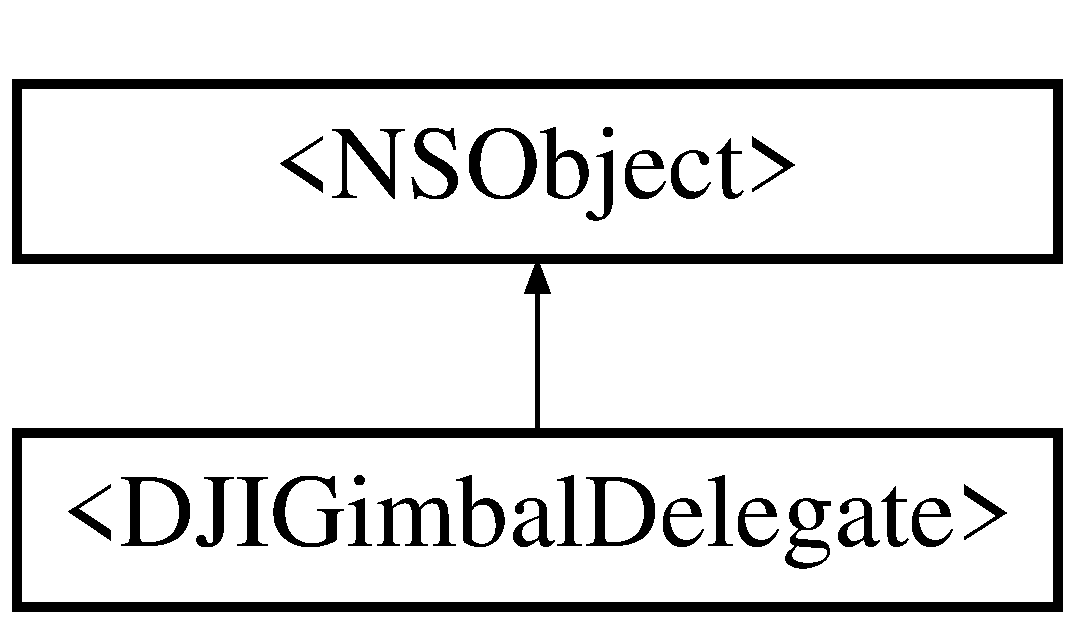
\includegraphics[height=2.000000cm]{protocol_d_j_i_gimbal_delegate-p}
\end{center}
\end{figure}
\subsection*{Instance Methods}
\begin{DoxyCompactItemize}
\item 
\hypertarget{protocol_d_j_i_gimbal_delegate-p_ac1566e085c2f2a420df609c8805f141b}{(void) -\/ {\bfseries gimbal\+Controller\+:did\+Gimbal\+Error\+:}}\label{protocol_d_j_i_gimbal_delegate-p_ac1566e085c2f2a420df609c8805f141b}

\end{DoxyCompactItemize}


The documentation for this protocol was generated from the following file\+:\begin{DoxyCompactItemize}
\item 
D\+J\+I\+Gimbal.\+h\end{DoxyCompactItemize}

\hypertarget{struct_d_j_i_gimbal_rotation}{\section{D\+J\+I\+Gimbal\+Rotation Struct Reference}
\label{struct_d_j_i_gimbal_rotation}\index{D\+J\+I\+Gimbal\+Rotation@{D\+J\+I\+Gimbal\+Rotation}}
}
\subsection*{Protected Attributes}
\begin{DoxyCompactItemize}
\item 
B\+O\+O\+L \hyperlink{struct_d_j_i_gimbal_rotation_ad6555675f7a142ff111b99d3ae214a5c}{enable}
\item 
int \hyperlink{struct_d_j_i_gimbal_rotation_abbcc4b75198c5a4b913ad1c61c47e787}{angle}
\item 
D\+J\+I\+Gimbal\+Rotation\+Angle\+Type \hyperlink{struct_d_j_i_gimbal_rotation_a819cec735930ba905d227b6a73f55d56}{angle\+Type}
\item 
D\+J\+I\+Gimbal\+Rotation\+Direction \hyperlink{struct_d_j_i_gimbal_rotation_aeda6599ce4fbdd86a7a474e481f601ac}{direction}
\end{DoxyCompactItemize}


\subsection{Member Data Documentation}
\hypertarget{struct_d_j_i_gimbal_rotation_abbcc4b75198c5a4b913ad1c61c47e787}{\index{D\+J\+I\+Gimbal\+Rotation@{D\+J\+I\+Gimbal\+Rotation}!angle@{angle}}
\index{angle@{angle}!D\+J\+I\+Gimbal\+Rotation@{D\+J\+I\+Gimbal\+Rotation}}
\subsubsection[{angle}]{\setlength{\rightskip}{0pt plus 5cm}-\/ (int) angle\hspace{0.3cm}{\ttfamily [protected]}}}\label{struct_d_j_i_gimbal_rotation_abbcc4b75198c5a4b913ad1c61c47e787}
The gimbal rotation angle. \hypertarget{struct_d_j_i_gimbal_rotation_a819cec735930ba905d227b6a73f55d56}{\index{D\+J\+I\+Gimbal\+Rotation@{D\+J\+I\+Gimbal\+Rotation}!angle\+Type@{angle\+Type}}
\index{angle\+Type@{angle\+Type}!D\+J\+I\+Gimbal\+Rotation@{D\+J\+I\+Gimbal\+Rotation}}
\subsubsection[{angle\+Type}]{\setlength{\rightskip}{0pt plus 5cm}-\/ (D\+J\+I\+Gimbal\+Rotation\+Angle\+Type) angle\+Type\hspace{0.3cm}{\ttfamily [protected]}}}\label{struct_d_j_i_gimbal_rotation_a819cec735930ba905d227b6a73f55d56}
The gimbal rotation type \hypertarget{struct_d_j_i_gimbal_rotation_aeda6599ce4fbdd86a7a474e481f601ac}{\index{D\+J\+I\+Gimbal\+Rotation@{D\+J\+I\+Gimbal\+Rotation}!direction@{direction}}
\index{direction@{direction}!D\+J\+I\+Gimbal\+Rotation@{D\+J\+I\+Gimbal\+Rotation}}
\subsubsection[{direction}]{\setlength{\rightskip}{0pt plus 5cm}-\/ (D\+J\+I\+Gimbal\+Rotation\+Direction) direction\hspace{0.3cm}{\ttfamily [protected]}}}\label{struct_d_j_i_gimbal_rotation_aeda6599ce4fbdd86a7a474e481f601ac}
The gimbal rotation direction \hypertarget{struct_d_j_i_gimbal_rotation_ad6555675f7a142ff111b99d3ae214a5c}{\index{D\+J\+I\+Gimbal\+Rotation@{D\+J\+I\+Gimbal\+Rotation}!enable@{enable}}
\index{enable@{enable}!D\+J\+I\+Gimbal\+Rotation@{D\+J\+I\+Gimbal\+Rotation}}
\subsubsection[{enable}]{\setlength{\rightskip}{0pt plus 5cm}-\/ (B\+O\+O\+L) enable\hspace{0.3cm}{\ttfamily [protected]}}}\label{struct_d_j_i_gimbal_rotation_ad6555675f7a142ff111b99d3ae214a5c}
The gimbal is rotation enable. 

The documentation for this struct was generated from the following file\+:\begin{DoxyCompactItemize}
\item 
D\+J\+I\+Gimbal.\+h\end{DoxyCompactItemize}

\hypertarget{protocol_d_j_i_ground_station-p}{\section{$<$D\+J\+I\+Ground\+Station$>$ Protocol Reference}
\label{protocol_d_j_i_ground_station-p}\index{$<$\+D\+J\+I\+Ground\+Station$>$@{$<$\+D\+J\+I\+Ground\+Station$>$}}
}
Inheritance diagram for $<$D\+J\+I\+Ground\+Station$>$\+:\begin{figure}[H]
\begin{center}
\leavevmode
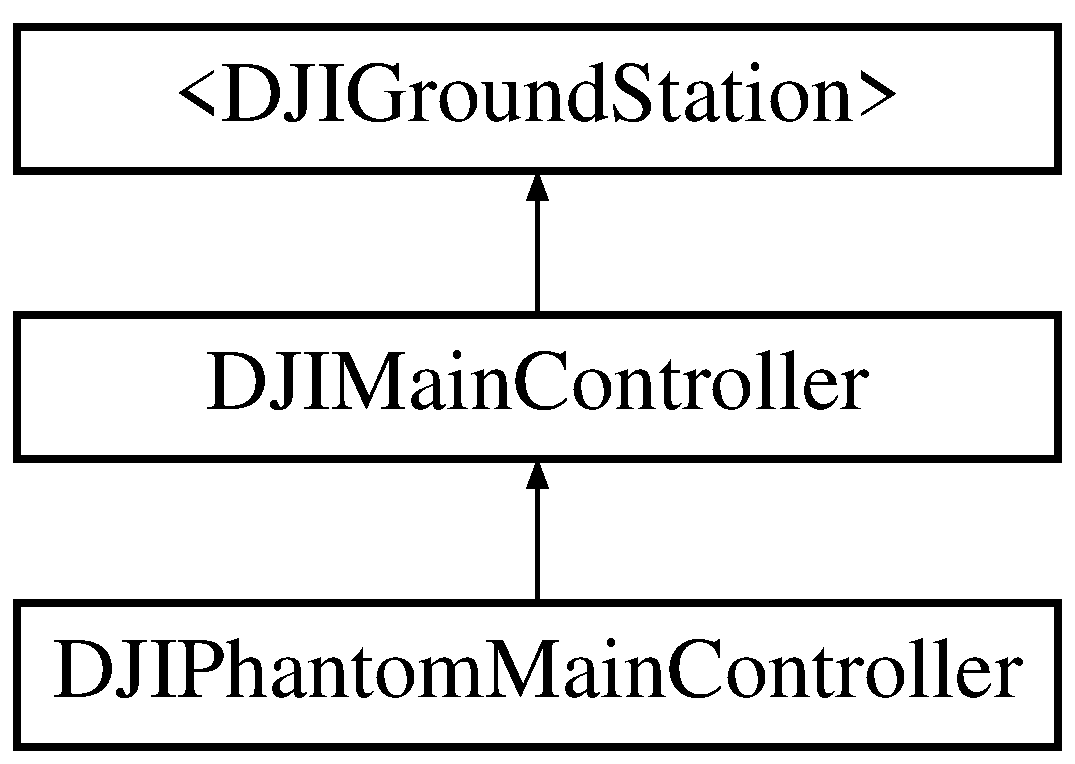
\includegraphics[height=3.000000cm]{protocol_d_j_i_ground_station-p}
\end{center}
\end{figure}
\subsection*{Instance Methods}
\begin{DoxyCompactItemize}
\item 
(void) -\/ \hyperlink{protocol_d_j_i_ground_station-p_a40c95668389564fabc888728e3a41fdd}{open\+Ground\+Station}
\item 
(void) -\/ \hyperlink{protocol_d_j_i_ground_station-p_a8277820cbee7b21d66f6b451b3490929}{close\+Ground\+Station}
\item 
(void) -\/ \hyperlink{protocol_d_j_i_ground_station-p_ab97ecb07317f961ffdf3a9fa8c49cf93}{upload\+Ground\+Station\+Task\+:}
\item 
(void) -\/ \hyperlink{protocol_d_j_i_ground_station-p_a025e4e9ff19bb0a587da014d36dcb1ad}{download\+Ground\+Station\+Task}
\item 
(void) -\/ \hyperlink{protocol_d_j_i_ground_station-p_adcdbcd7826de846abbcb6aa7dd370cce}{start\+Ground\+Station\+Task}
\item 
(void) -\/ \hyperlink{protocol_d_j_i_ground_station-p_a20b05354a058a92bd3e9299f8789df51}{pause\+Ground\+Station\+Task}
\item 
(void) -\/ \hyperlink{protocol_d_j_i_ground_station-p_ac8cc4c027e84e00470e6b66e30b1d0b6}{continue\+Ground\+Station\+Task}
\item 
(void) -\/ \hyperlink{protocol_d_j_i_ground_station-p_a7e98c94e54d37dffa04af4725f4e4dc9}{gohome}
\item 
(B\+O\+O\+L) -\/ \hyperlink{protocol_d_j_i_ground_station-p_a5a673afff4673f9bb76db0ad81b0bc96}{set\+Aircraft\+Pitch\+Speed\+:}
\item 
(B\+O\+O\+L) -\/ \hyperlink{protocol_d_j_i_ground_station-p_a252a8ba557644867ebd9c5a9af4a06ac}{set\+Aircraft\+Roll\+Speed\+:}
\item 
(B\+O\+O\+L) -\/ \hyperlink{protocol_d_j_i_ground_station-p_a48d6a1e3162e44f045d8542912ff5b9a}{set\+Aircraft\+Yaw\+Speed\+:}
\item 
(B\+O\+O\+L) -\/ \hyperlink{protocol_d_j_i_ground_station-p_a426d344c5747117275fbbeb94d0cfac2}{set\+Aircraft\+Throttle\+:}
\item 
(B\+O\+O\+L) -\/ \hyperlink{protocol_d_j_i_ground_station-p_ac9087399fe652fa5e50d402113db73f9}{set\+Aircraft\+Joystick\+With\+Pitch\+:\+Roll\+:\+Yaw\+:\+Throttle\+:}
\end{DoxyCompactItemize}
\subsection*{Properties}
\begin{DoxyCompactItemize}
\item 
\hypertarget{protocol_d_j_i_ground_station-p_a2302bca047813b8e4384488f87d32acd}{id$<$ Ground\+Station\+Delegate $>$ {\bfseries ground\+Station\+Delegate}}\label{protocol_d_j_i_ground_station-p_a2302bca047813b8e4384488f87d32acd}

\item 
\hypertarget{protocol_d_j_i_ground_station-p_ab9ed01091b03fb8aaafa2dba4891e899}{\hyperlink{interface_d_j_i_ground_station_task}{D\+J\+I\+Ground\+Station\+Task} $\ast$ {\bfseries ground\+Station\+Task}}\label{protocol_d_j_i_ground_station-p_ab9ed01091b03fb8aaafa2dba4891e899}

\end{DoxyCompactItemize}


\subsection{Method Documentation}
\hypertarget{protocol_d_j_i_ground_station-p_a8277820cbee7b21d66f6b451b3490929}{\index{D\+J\+I\+Ground\+Station-\/p@{D\+J\+I\+Ground\+Station-\/p}!close\+Ground\+Station@{close\+Ground\+Station}}
\index{close\+Ground\+Station@{close\+Ground\+Station}!D\+J\+I\+Ground\+Station-\/p@{D\+J\+I\+Ground\+Station-\/p}}
\subsubsection[{close\+Ground\+Station}]{\setlength{\rightskip}{0pt plus 5cm}-\/ (void) close\+Ground\+Station 
\begin{DoxyParamCaption}
{}
\end{DoxyParamCaption}
}}\label{protocol_d_j_i_ground_station-p_a8277820cbee7b21d66f6b451b3490929}
Close ground station \hypertarget{protocol_d_j_i_ground_station-p_ac8cc4c027e84e00470e6b66e30b1d0b6}{\index{D\+J\+I\+Ground\+Station-\/p@{D\+J\+I\+Ground\+Station-\/p}!continue\+Ground\+Station\+Task@{continue\+Ground\+Station\+Task}}
\index{continue\+Ground\+Station\+Task@{continue\+Ground\+Station\+Task}!D\+J\+I\+Ground\+Station-\/p@{D\+J\+I\+Ground\+Station-\/p}}
\subsubsection[{continue\+Ground\+Station\+Task}]{\setlength{\rightskip}{0pt plus 5cm}-\/ (void) continue\+Ground\+Station\+Task 
\begin{DoxyParamCaption}
{}
\end{DoxyParamCaption}
}}\label{protocol_d_j_i_ground_station-p_ac8cc4c027e84e00470e6b66e30b1d0b6}
Continue task \hypertarget{protocol_d_j_i_ground_station-p_a025e4e9ff19bb0a587da014d36dcb1ad}{\index{D\+J\+I\+Ground\+Station-\/p@{D\+J\+I\+Ground\+Station-\/p}!download\+Ground\+Station\+Task@{download\+Ground\+Station\+Task}}
\index{download\+Ground\+Station\+Task@{download\+Ground\+Station\+Task}!D\+J\+I\+Ground\+Station-\/p@{D\+J\+I\+Ground\+Station-\/p}}
\subsubsection[{download\+Ground\+Station\+Task}]{\setlength{\rightskip}{0pt plus 5cm}-\/ (void) download\+Ground\+Station\+Task 
\begin{DoxyParamCaption}
{}
\end{DoxyParamCaption}
}}\label{protocol_d_j_i_ground_station-p_a025e4e9ff19bb0a587da014d36dcb1ad}
Download ground station task, if no task on the airplane, property \char`\"{}ground\+Station\+Task\char`\"{} will be set to nil. \hypertarget{protocol_d_j_i_ground_station-p_a7e98c94e54d37dffa04af4725f4e4dc9}{\index{D\+J\+I\+Ground\+Station-\/p@{D\+J\+I\+Ground\+Station-\/p}!gohome@{gohome}}
\index{gohome@{gohome}!D\+J\+I\+Ground\+Station-\/p@{D\+J\+I\+Ground\+Station-\/p}}
\subsubsection[{gohome}]{\setlength{\rightskip}{0pt plus 5cm}-\/ (void) gohome 
\begin{DoxyParamCaption}
{}
\end{DoxyParamCaption}
}}\label{protocol_d_j_i_ground_station-p_a7e98c94e54d37dffa04af4725f4e4dc9}
Airplane go home \begin{DoxyAttention}{Attention}
the home point of the drone should had setup at the begining 
\end{DoxyAttention}
\hypertarget{protocol_d_j_i_ground_station-p_a40c95668389564fabc888728e3a41fdd}{\index{D\+J\+I\+Ground\+Station-\/p@{D\+J\+I\+Ground\+Station-\/p}!open\+Ground\+Station@{open\+Ground\+Station}}
\index{open\+Ground\+Station@{open\+Ground\+Station}!D\+J\+I\+Ground\+Station-\/p@{D\+J\+I\+Ground\+Station-\/p}}
\subsubsection[{open\+Ground\+Station}]{\setlength{\rightskip}{0pt plus 5cm}-\/ (void) open\+Ground\+Station 
\begin{DoxyParamCaption}
{}
\end{DoxyParamCaption}
}}\label{protocol_d_j_i_ground_station-p_a40c95668389564fabc888728e3a41fdd}
Open ground station \hypertarget{protocol_d_j_i_ground_station-p_a20b05354a058a92bd3e9299f8789df51}{\index{D\+J\+I\+Ground\+Station-\/p@{D\+J\+I\+Ground\+Station-\/p}!pause\+Ground\+Station\+Task@{pause\+Ground\+Station\+Task}}
\index{pause\+Ground\+Station\+Task@{pause\+Ground\+Station\+Task}!D\+J\+I\+Ground\+Station-\/p@{D\+J\+I\+Ground\+Station-\/p}}
\subsubsection[{pause\+Ground\+Station\+Task}]{\setlength{\rightskip}{0pt plus 5cm}-\/ (void) pause\+Ground\+Station\+Task 
\begin{DoxyParamCaption}
{}
\end{DoxyParamCaption}
}}\label{protocol_d_j_i_ground_station-p_a20b05354a058a92bd3e9299f8789df51}
Pause task, drone will hover at the current place. \hypertarget{protocol_d_j_i_ground_station-p_ac9087399fe652fa5e50d402113db73f9}{\index{D\+J\+I\+Ground\+Station-\/p@{D\+J\+I\+Ground\+Station-\/p}!set\+Aircraft\+Joystick\+With\+Pitch\+:\+Roll\+:\+Yaw\+:\+Throttle\+:@{set\+Aircraft\+Joystick\+With\+Pitch\+:\+Roll\+:\+Yaw\+:\+Throttle\+:}}
\index{set\+Aircraft\+Joystick\+With\+Pitch\+:\+Roll\+:\+Yaw\+:\+Throttle\+:@{set\+Aircraft\+Joystick\+With\+Pitch\+:\+Roll\+:\+Yaw\+:\+Throttle\+:}!D\+J\+I\+Ground\+Station-\/p@{D\+J\+I\+Ground\+Station-\/p}}
\subsubsection[{set\+Aircraft\+Joystick\+With\+Pitch\+:\+Roll\+:\+Yaw\+:\+Throttle\+:}]{\setlength{\rightskip}{0pt plus 5cm}-\/ (B\+O\+O\+L) set\+Aircraft\+Joystick\+With\+Pitch\+: 
\begin{DoxyParamCaption}
\item[{(int)}]{pitch}
\item[{Roll:(int)}]{roll}
\item[{Yaw:(int)}]{yaw}
\item[{Throttle:(int)}]{throttle}
\end{DoxyParamCaption}
}}\label{protocol_d_j_i_ground_station-p_ac9087399fe652fa5e50d402113db73f9}
Set aricraft joystick.


\begin{DoxyParams}{Parameters}
{\em pitch} & Pitch speed between \mbox{[}-\/1000, 1000\mbox{]} \\
\hline
{\em roll} & Roll speed between \mbox{[}-\/1000, 1000\mbox{]} \\
\hline
{\em yaw} & Yaw speed between \mbox{[}-\/1000, 1000\mbox{]} \\
\hline
{\em throttl} & Throttl \mbox{[}0 stop, 1 up, 2 down\mbox{]} \\
\hline
\end{DoxyParams}
\begin{DoxyAttention}{Attention}
This api is valid only after the drone is pausing. 
\end{DoxyAttention}
\hypertarget{protocol_d_j_i_ground_station-p_a5a673afff4673f9bb76db0ad81b0bc96}{\index{D\+J\+I\+Ground\+Station-\/p@{D\+J\+I\+Ground\+Station-\/p}!set\+Aircraft\+Pitch\+Speed\+:@{set\+Aircraft\+Pitch\+Speed\+:}}
\index{set\+Aircraft\+Pitch\+Speed\+:@{set\+Aircraft\+Pitch\+Speed\+:}!D\+J\+I\+Ground\+Station-\/p@{D\+J\+I\+Ground\+Station-\/p}}
\subsubsection[{set\+Aircraft\+Pitch\+Speed\+:}]{\setlength{\rightskip}{0pt plus 5cm}-\/ (B\+O\+O\+L) set\+Aircraft\+Pitch\+Speed\+: 
\begin{DoxyParamCaption}
\item[{(int)}]{pitch\+Speed}
\end{DoxyParamCaption}
}}\label{protocol_d_j_i_ground_station-p_a5a673afff4673f9bb76db0ad81b0bc96}
Set aircraft pitch rotation speed


\begin{DoxyParams}{Parameters}
{\em pitch\+Speed} & Pitch speed between \mbox{[}-\/1000, 1000\mbox{]} \\
\hline
\end{DoxyParams}
\begin{DoxyAttention}{Attention}
This api is valid only after the drone is pausing. 
\end{DoxyAttention}
\hypertarget{protocol_d_j_i_ground_station-p_a252a8ba557644867ebd9c5a9af4a06ac}{\index{D\+J\+I\+Ground\+Station-\/p@{D\+J\+I\+Ground\+Station-\/p}!set\+Aircraft\+Roll\+Speed\+:@{set\+Aircraft\+Roll\+Speed\+:}}
\index{set\+Aircraft\+Roll\+Speed\+:@{set\+Aircraft\+Roll\+Speed\+:}!D\+J\+I\+Ground\+Station-\/p@{D\+J\+I\+Ground\+Station-\/p}}
\subsubsection[{set\+Aircraft\+Roll\+Speed\+:}]{\setlength{\rightskip}{0pt plus 5cm}-\/ (B\+O\+O\+L) set\+Aircraft\+Roll\+Speed\+: 
\begin{DoxyParamCaption}
\item[{(int)}]{roll\+Speed}
\end{DoxyParamCaption}
}}\label{protocol_d_j_i_ground_station-p_a252a8ba557644867ebd9c5a9af4a06ac}
Set aircraft roll rotation speed


\begin{DoxyParams}{Parameters}
{\em roll\+Speed} & Roll speed between \mbox{[}-\/1000, 1000\mbox{]} \\
\hline
\end{DoxyParams}
\begin{DoxyAttention}{Attention}
This api is valid only after the drone is pausing. 
\end{DoxyAttention}
\hypertarget{protocol_d_j_i_ground_station-p_a426d344c5747117275fbbeb94d0cfac2}{\index{D\+J\+I\+Ground\+Station-\/p@{D\+J\+I\+Ground\+Station-\/p}!set\+Aircraft\+Throttle\+:@{set\+Aircraft\+Throttle\+:}}
\index{set\+Aircraft\+Throttle\+:@{set\+Aircraft\+Throttle\+:}!D\+J\+I\+Ground\+Station-\/p@{D\+J\+I\+Ground\+Station-\/p}}
\subsubsection[{set\+Aircraft\+Throttle\+:}]{\setlength{\rightskip}{0pt plus 5cm}-\/ (B\+O\+O\+L) set\+Aircraft\+Throttle\+: 
\begin{DoxyParamCaption}
\item[{(int)}]{throttle}
\end{DoxyParamCaption}
}}\label{protocol_d_j_i_ground_station-p_a426d344c5747117275fbbeb94d0cfac2}
Set aircraft throttle


\begin{DoxyParams}{Parameters}
{\em throttl} & Throttle value \mbox{[}0 stop, 1 up, 2 down\mbox{]} \\
\hline
\end{DoxyParams}
\hypertarget{protocol_d_j_i_ground_station-p_a48d6a1e3162e44f045d8542912ff5b9a}{\index{D\+J\+I\+Ground\+Station-\/p@{D\+J\+I\+Ground\+Station-\/p}!set\+Aircraft\+Yaw\+Speed\+:@{set\+Aircraft\+Yaw\+Speed\+:}}
\index{set\+Aircraft\+Yaw\+Speed\+:@{set\+Aircraft\+Yaw\+Speed\+:}!D\+J\+I\+Ground\+Station-\/p@{D\+J\+I\+Ground\+Station-\/p}}
\subsubsection[{set\+Aircraft\+Yaw\+Speed\+:}]{\setlength{\rightskip}{0pt plus 5cm}-\/ (B\+O\+O\+L) set\+Aircraft\+Yaw\+Speed\+: 
\begin{DoxyParamCaption}
\item[{(int)}]{yaw\+Speed}
\end{DoxyParamCaption}
}}\label{protocol_d_j_i_ground_station-p_a48d6a1e3162e44f045d8542912ff5b9a}
Set aircraft yaw rotation speed


\begin{DoxyParams}{Parameters}
{\em yaw\+Speed} & Yaw speed between \mbox{[}-\/1000, 1000\mbox{]} \\
\hline
\end{DoxyParams}
\begin{DoxyAttention}{Attention}
This api is valid only after the drone is pausing. 
\end{DoxyAttention}
\hypertarget{protocol_d_j_i_ground_station-p_adcdbcd7826de846abbcb6aa7dd370cce}{\index{D\+J\+I\+Ground\+Station-\/p@{D\+J\+I\+Ground\+Station-\/p}!start\+Ground\+Station\+Task@{start\+Ground\+Station\+Task}}
\index{start\+Ground\+Station\+Task@{start\+Ground\+Station\+Task}!D\+J\+I\+Ground\+Station-\/p@{D\+J\+I\+Ground\+Station-\/p}}
\subsubsection[{start\+Ground\+Station\+Task}]{\setlength{\rightskip}{0pt plus 5cm}-\/ (void) start\+Ground\+Station\+Task 
\begin{DoxyParamCaption}
{}
\end{DoxyParamCaption}
}}\label{protocol_d_j_i_ground_station-p_adcdbcd7826de846abbcb6aa7dd370cce}
Start executing task on the drone, if the airplane not takeoff, it will takeoff automatically and execute the task. \hypertarget{protocol_d_j_i_ground_station-p_ab97ecb07317f961ffdf3a9fa8c49cf93}{\index{D\+J\+I\+Ground\+Station-\/p@{D\+J\+I\+Ground\+Station-\/p}!upload\+Ground\+Station\+Task\+:@{upload\+Ground\+Station\+Task\+:}}
\index{upload\+Ground\+Station\+Task\+:@{upload\+Ground\+Station\+Task\+:}!D\+J\+I\+Ground\+Station-\/p@{D\+J\+I\+Ground\+Station-\/p}}
\subsubsection[{upload\+Ground\+Station\+Task\+:}]{\setlength{\rightskip}{0pt plus 5cm}-\/ (void) upload\+Ground\+Station\+Task\+: 
\begin{DoxyParamCaption}
\item[{({\bf D\+J\+I\+Ground\+Station\+Task} $\ast$)}]{task}
\end{DoxyParamCaption}
}}\label{protocol_d_j_i_ground_station-p_ab97ecb07317f961ffdf3a9fa8c49cf93}
Upload a new task to the airplane.


\begin{DoxyParams}{Parameters}
{\em task} & \\
\hline
\end{DoxyParams}


The documentation for this protocol was generated from the following file\+:\begin{DoxyCompactItemize}
\item 
D\+J\+I\+Ground\+Station.\+h\end{DoxyCompactItemize}

\hypertarget{interface_d_j_i_ground_station_flying_info}{\section{D\+J\+I\+Ground\+Station\+Flying\+Info Class Reference}
\label{interface_d_j_i_ground_station_flying_info}\index{D\+J\+I\+Ground\+Station\+Flying\+Info@{D\+J\+I\+Ground\+Station\+Flying\+Info}}
}
Inheritance diagram for D\+J\+I\+Ground\+Station\+Flying\+Info\+:\begin{figure}[H]
\begin{center}
\leavevmode
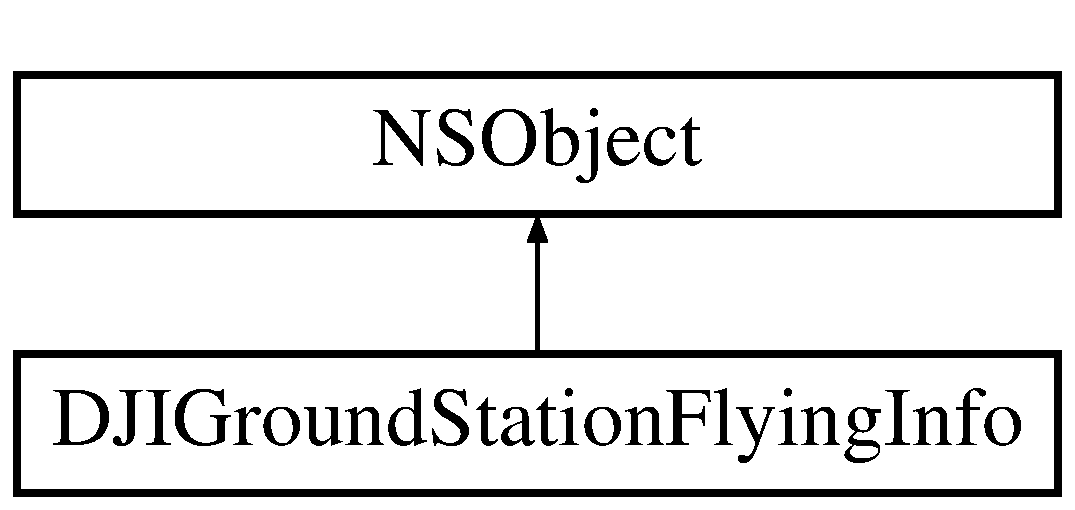
\includegraphics[height=2.000000cm]{interface_d_j_i_ground_station_flying_info}
\end{center}
\end{figure}
\subsection*{Properties}
\begin{DoxyCompactItemize}
\item 
int \hyperlink{interface_d_j_i_ground_station_flying_info_a1ee65df6fec56e23c545f2a9bea7cf8b}{target\+Waypoint\+Index}
\item 
int \hyperlink{interface_d_j_i_ground_station_flying_info_aab354d5d7dbe977708da7976adf98452}{satellite\+Count}
\item 
C\+L\+Location\+Coordinate2\+D \hyperlink{interface_d_j_i_ground_station_flying_info_aa578b0630c020c9dbfb8a990fbe7a072}{home\+Location}
\item 
C\+L\+Location\+Coordinate2\+D \hyperlink{interface_d_j_i_ground_station_flying_info_aefaed815db457c38924ccae0a7ce4f7d}{drone\+Location}
\item 
C\+L\+Location\+Coordinate2\+D \hyperlink{interface_d_j_i_ground_station_flying_info_ac9a21f003ac25353be2de2e3505a17e5}{target\+Waypoint\+Location}
\item 
float \hyperlink{interface_d_j_i_ground_station_flying_info_ad8b985803c6a5bb238db09c9269d8691}{velocity\+X}
\item 
float \hyperlink{interface_d_j_i_ground_station_flying_info_a9e47f0ef8b8b59e2b7715cd186c41337}{velocity\+Y}
\item 
float \hyperlink{interface_d_j_i_ground_station_flying_info_a407350d0d50e83823e5ab856cb06d1d2}{velocity\+Z}
\item 
float \hyperlink{interface_d_j_i_ground_station_flying_info_a3a3af4721948773c4f003b129688dbd6}{altitude}
\item 
float \hyperlink{interface_d_j_i_ground_station_flying_info_a8a65f801952f96869b40cd3028ab54d4}{target\+Altitude}
\item 
\hyperlink{struct_d_j_i_attitude}{D\+J\+I\+Attitude} \hyperlink{interface_d_j_i_ground_station_flying_info_abd7294b2a74c6d5b1944cbad0801e732}{attitude}
\item 
Ground\+Station\+Control\+Mode \hyperlink{interface_d_j_i_ground_station_flying_info_a6a306041d30a49578feb95b33afe930e}{control\+Mode}
\item 
Ground\+Station\+Gps\+Status \hyperlink{interface_d_j_i_ground_station_flying_info_a2d16a3fe7607265429b2d9e435abe895}{gps\+Status}
\item 
Ground\+Station\+Drone\+Status \hyperlink{interface_d_j_i_ground_station_flying_info_ab43f7fde7a1b31650294e52eabc5ab23}{drone\+Status}
\end{DoxyCompactItemize}


\subsection{Property Documentation}
\hypertarget{interface_d_j_i_ground_station_flying_info_a3a3af4721948773c4f003b129688dbd6}{\index{D\+J\+I\+Ground\+Station\+Flying\+Info@{D\+J\+I\+Ground\+Station\+Flying\+Info}!altitude@{altitude}}
\index{altitude@{altitude}!D\+J\+I\+Ground\+Station\+Flying\+Info@{D\+J\+I\+Ground\+Station\+Flying\+Info}}
\subsubsection[{altitude}]{\setlength{\rightskip}{0pt plus 5cm}-\/ (float) altitude\hspace{0.3cm}{\ttfamily [read]}, {\ttfamily [nonatomic]}, {\ttfamily [assign]}}}\label{interface_d_j_i_ground_station_flying_info_a3a3af4721948773c4f003b129688dbd6}
Altitude of the drone, (0.\+1m) \hypertarget{interface_d_j_i_ground_station_flying_info_abd7294b2a74c6d5b1944cbad0801e732}{\index{D\+J\+I\+Ground\+Station\+Flying\+Info@{D\+J\+I\+Ground\+Station\+Flying\+Info}!attitude@{attitude}}
\index{attitude@{attitude}!D\+J\+I\+Ground\+Station\+Flying\+Info@{D\+J\+I\+Ground\+Station\+Flying\+Info}}
\subsubsection[{attitude}]{\setlength{\rightskip}{0pt plus 5cm}-\/ ({\bf D\+J\+I\+Attitude}) attitude\hspace{0.3cm}{\ttfamily [read]}, {\ttfamily [nonatomic]}, {\ttfamily [assign]}}}\label{interface_d_j_i_ground_station_flying_info_abd7294b2a74c6d5b1944cbad0801e732}
Attitude of the drone \hypertarget{interface_d_j_i_ground_station_flying_info_a6a306041d30a49578feb95b33afe930e}{\index{D\+J\+I\+Ground\+Station\+Flying\+Info@{D\+J\+I\+Ground\+Station\+Flying\+Info}!control\+Mode@{control\+Mode}}
\index{control\+Mode@{control\+Mode}!D\+J\+I\+Ground\+Station\+Flying\+Info@{D\+J\+I\+Ground\+Station\+Flying\+Info}}
\subsubsection[{control\+Mode}]{\setlength{\rightskip}{0pt plus 5cm}-\/ (Ground\+Station\+Control\+Mode) control\+Mode\hspace{0.3cm}{\ttfamily [read]}, {\ttfamily [nonatomic]}, {\ttfamily [assign]}}}\label{interface_d_j_i_ground_station_flying_info_a6a306041d30a49578feb95b33afe930e}
Control mode \hypertarget{interface_d_j_i_ground_station_flying_info_aefaed815db457c38924ccae0a7ce4f7d}{\index{D\+J\+I\+Ground\+Station\+Flying\+Info@{D\+J\+I\+Ground\+Station\+Flying\+Info}!drone\+Location@{drone\+Location}}
\index{drone\+Location@{drone\+Location}!D\+J\+I\+Ground\+Station\+Flying\+Info@{D\+J\+I\+Ground\+Station\+Flying\+Info}}
\subsubsection[{drone\+Location}]{\setlength{\rightskip}{0pt plus 5cm}-\/ (C\+L\+Location\+Coordinate2\+D) drone\+Location\hspace{0.3cm}{\ttfamily [read]}, {\ttfamily [nonatomic]}, {\ttfamily [assign]}}}\label{interface_d_j_i_ground_station_flying_info_aefaed815db457c38924ccae0a7ce4f7d}
Current location of the drone \hypertarget{interface_d_j_i_ground_station_flying_info_ab43f7fde7a1b31650294e52eabc5ab23}{\index{D\+J\+I\+Ground\+Station\+Flying\+Info@{D\+J\+I\+Ground\+Station\+Flying\+Info}!drone\+Status@{drone\+Status}}
\index{drone\+Status@{drone\+Status}!D\+J\+I\+Ground\+Station\+Flying\+Info@{D\+J\+I\+Ground\+Station\+Flying\+Info}}
\subsubsection[{drone\+Status}]{\setlength{\rightskip}{0pt plus 5cm}-\/ (Ground\+Station\+Drone\+Status) drone\+Status\hspace{0.3cm}{\ttfamily [read]}, {\ttfamily [nonatomic]}, {\ttfamily [assign]}}}\label{interface_d_j_i_ground_station_flying_info_ab43f7fde7a1b31650294e52eabc5ab23}
Drone status\+: \hypertarget{interface_d_j_i_ground_station_flying_info_a2d16a3fe7607265429b2d9e435abe895}{\index{D\+J\+I\+Ground\+Station\+Flying\+Info@{D\+J\+I\+Ground\+Station\+Flying\+Info}!gps\+Status@{gps\+Status}}
\index{gps\+Status@{gps\+Status}!D\+J\+I\+Ground\+Station\+Flying\+Info@{D\+J\+I\+Ground\+Station\+Flying\+Info}}
\subsubsection[{gps\+Status}]{\setlength{\rightskip}{0pt plus 5cm}-\/ (Ground\+Station\+Gps\+Status) gps\+Status\hspace{0.3cm}{\ttfamily [read]}, {\ttfamily [nonatomic]}, {\ttfamily [assign]}}}\label{interface_d_j_i_ground_station_flying_info_a2d16a3fe7607265429b2d9e435abe895}
Gps status \+: good, weak, bad \hypertarget{interface_d_j_i_ground_station_flying_info_aa578b0630c020c9dbfb8a990fbe7a072}{\index{D\+J\+I\+Ground\+Station\+Flying\+Info@{D\+J\+I\+Ground\+Station\+Flying\+Info}!home\+Location@{home\+Location}}
\index{home\+Location@{home\+Location}!D\+J\+I\+Ground\+Station\+Flying\+Info@{D\+J\+I\+Ground\+Station\+Flying\+Info}}
\subsubsection[{home\+Location}]{\setlength{\rightskip}{0pt plus 5cm}-\/ (C\+L\+Location\+Coordinate2\+D) home\+Location\hspace{0.3cm}{\ttfamily [read]}, {\ttfamily [nonatomic]}, {\ttfamily [assign]}}}\label{interface_d_j_i_ground_station_flying_info_aa578b0630c020c9dbfb8a990fbe7a072}
Home point \hypertarget{interface_d_j_i_ground_station_flying_info_aab354d5d7dbe977708da7976adf98452}{\index{D\+J\+I\+Ground\+Station\+Flying\+Info@{D\+J\+I\+Ground\+Station\+Flying\+Info}!satellite\+Count@{satellite\+Count}}
\index{satellite\+Count@{satellite\+Count}!D\+J\+I\+Ground\+Station\+Flying\+Info@{D\+J\+I\+Ground\+Station\+Flying\+Info}}
\subsubsection[{satellite\+Count}]{\setlength{\rightskip}{0pt plus 5cm}-\/ (int) satellite\+Count\hspace{0.3cm}{\ttfamily [read]}, {\ttfamily [nonatomic]}, {\ttfamily [assign]}}}\label{interface_d_j_i_ground_station_flying_info_aab354d5d7dbe977708da7976adf98452}
Satellite count. if the satellite\+Count $>$= 6, home point will be set \hypertarget{interface_d_j_i_ground_station_flying_info_a8a65f801952f96869b40cd3028ab54d4}{\index{D\+J\+I\+Ground\+Station\+Flying\+Info@{D\+J\+I\+Ground\+Station\+Flying\+Info}!target\+Altitude@{target\+Altitude}}
\index{target\+Altitude@{target\+Altitude}!D\+J\+I\+Ground\+Station\+Flying\+Info@{D\+J\+I\+Ground\+Station\+Flying\+Info}}
\subsubsection[{target\+Altitude}]{\setlength{\rightskip}{0pt plus 5cm}-\/ (float) target\+Altitude\hspace{0.3cm}{\ttfamily [read]}, {\ttfamily [nonatomic]}, {\ttfamily [assign]}}}\label{interface_d_j_i_ground_station_flying_info_a8a65f801952f96869b40cd3028ab54d4}
The target altitude will flying to (0.\+1m) \hypertarget{interface_d_j_i_ground_station_flying_info_a1ee65df6fec56e23c545f2a9bea7cf8b}{\index{D\+J\+I\+Ground\+Station\+Flying\+Info@{D\+J\+I\+Ground\+Station\+Flying\+Info}!target\+Waypoint\+Index@{target\+Waypoint\+Index}}
\index{target\+Waypoint\+Index@{target\+Waypoint\+Index}!D\+J\+I\+Ground\+Station\+Flying\+Info@{D\+J\+I\+Ground\+Station\+Flying\+Info}}
\subsubsection[{target\+Waypoint\+Index}]{\setlength{\rightskip}{0pt plus 5cm}-\/ (int) target\+Waypoint\+Index\hspace{0.3cm}{\ttfamily [read]}, {\ttfamily [nonatomic]}, {\ttfamily [assign]}}}\label{interface_d_j_i_ground_station_flying_info_a1ee65df6fec56e23c545f2a9bea7cf8b}
Target waypoint index that will flying to. -\/1 if the task not start \hypertarget{interface_d_j_i_ground_station_flying_info_ac9a21f003ac25353be2de2e3505a17e5}{\index{D\+J\+I\+Ground\+Station\+Flying\+Info@{D\+J\+I\+Ground\+Station\+Flying\+Info}!target\+Waypoint\+Location@{target\+Waypoint\+Location}}
\index{target\+Waypoint\+Location@{target\+Waypoint\+Location}!D\+J\+I\+Ground\+Station\+Flying\+Info@{D\+J\+I\+Ground\+Station\+Flying\+Info}}
\subsubsection[{target\+Waypoint\+Location}]{\setlength{\rightskip}{0pt plus 5cm}-\/ (C\+L\+Location\+Coordinate2\+D) target\+Waypoint\+Location\hspace{0.3cm}{\ttfamily [read]}, {\ttfamily [nonatomic]}, {\ttfamily [assign]}}}\label{interface_d_j_i_ground_station_flying_info_ac9a21f003ac25353be2de2e3505a17e5}
The target waypoint location will flying to \hypertarget{interface_d_j_i_ground_station_flying_info_ad8b985803c6a5bb238db09c9269d8691}{\index{D\+J\+I\+Ground\+Station\+Flying\+Info@{D\+J\+I\+Ground\+Station\+Flying\+Info}!velocity\+X@{velocity\+X}}
\index{velocity\+X@{velocity\+X}!D\+J\+I\+Ground\+Station\+Flying\+Info@{D\+J\+I\+Ground\+Station\+Flying\+Info}}
\subsubsection[{velocity\+X}]{\setlength{\rightskip}{0pt plus 5cm}-\/ (float) velocity\+X\hspace{0.3cm}{\ttfamily [read]}, {\ttfamily [nonatomic]}, {\ttfamily [assign]}}}\label{interface_d_j_i_ground_station_flying_info_ad8b985803c6a5bb238db09c9269d8691}
Speed on x (m/s) \hypertarget{interface_d_j_i_ground_station_flying_info_a9e47f0ef8b8b59e2b7715cd186c41337}{\index{D\+J\+I\+Ground\+Station\+Flying\+Info@{D\+J\+I\+Ground\+Station\+Flying\+Info}!velocity\+Y@{velocity\+Y}}
\index{velocity\+Y@{velocity\+Y}!D\+J\+I\+Ground\+Station\+Flying\+Info@{D\+J\+I\+Ground\+Station\+Flying\+Info}}
\subsubsection[{velocity\+Y}]{\setlength{\rightskip}{0pt plus 5cm}-\/ (float) velocity\+Y\hspace{0.3cm}{\ttfamily [read]}, {\ttfamily [nonatomic]}, {\ttfamily [assign]}}}\label{interface_d_j_i_ground_station_flying_info_a9e47f0ef8b8b59e2b7715cd186c41337}
Speed on y (m/s) \hypertarget{interface_d_j_i_ground_station_flying_info_a407350d0d50e83823e5ab856cb06d1d2}{\index{D\+J\+I\+Ground\+Station\+Flying\+Info@{D\+J\+I\+Ground\+Station\+Flying\+Info}!velocity\+Z@{velocity\+Z}}
\index{velocity\+Z@{velocity\+Z}!D\+J\+I\+Ground\+Station\+Flying\+Info@{D\+J\+I\+Ground\+Station\+Flying\+Info}}
\subsubsection[{velocity\+Z}]{\setlength{\rightskip}{0pt plus 5cm}-\/ (float) velocity\+Z\hspace{0.3cm}{\ttfamily [read]}, {\ttfamily [nonatomic]}, {\ttfamily [assign]}}}\label{interface_d_j_i_ground_station_flying_info_a407350d0d50e83823e5ab856cb06d1d2}
Speed on z (m/s) 

The documentation for this class was generated from the following file\+:\begin{DoxyCompactItemize}
\item 
D\+J\+I\+Ground\+Station\+Flying\+Info.\+h\end{DoxyCompactItemize}

\hypertarget{interface_d_j_i_ground_station_task}{\section{D\+J\+I\+Ground\+Station\+Task Class Reference}
\label{interface_d_j_i_ground_station_task}\index{D\+J\+I\+Ground\+Station\+Task@{D\+J\+I\+Ground\+Station\+Task}}
}
Inheritance diagram for D\+J\+I\+Ground\+Station\+Task\+:\begin{figure}[H]
\begin{center}
\leavevmode
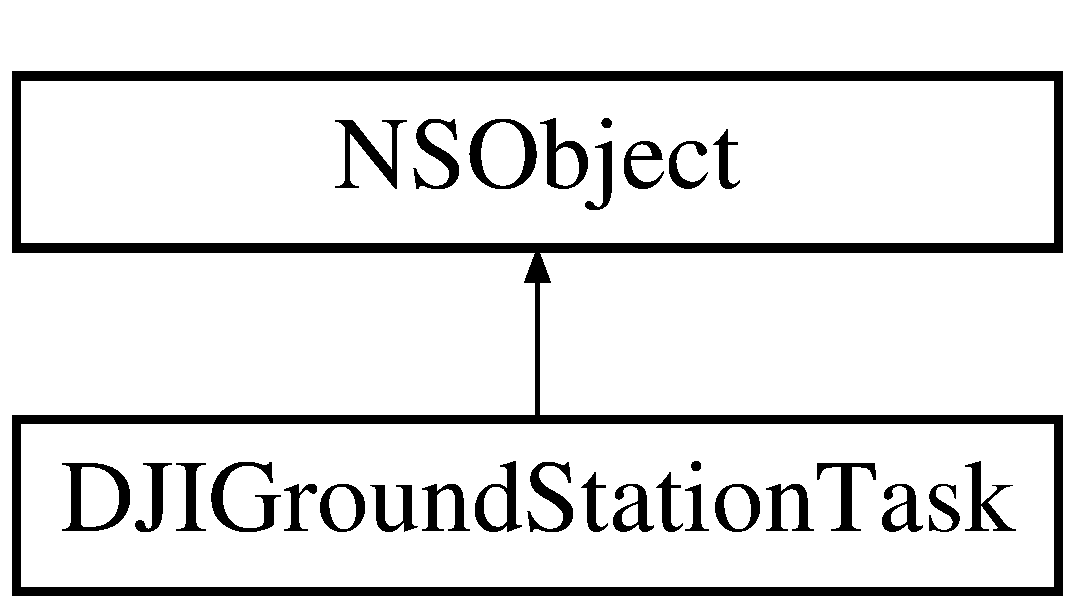
\includegraphics[height=2.000000cm]{interface_d_j_i_ground_station_task}
\end{center}
\end{figure}
\subsection*{Instance Methods}
\begin{DoxyCompactItemize}
\item 
(void) -\/ \hyperlink{interface_d_j_i_ground_station_task_a9f1a622c4e3282a17fb27fe0feaecb9a}{add\+Waypoint\+:}
\item 
(void) -\/ \hyperlink{interface_d_j_i_ground_station_task_a451503132beec02466927bb5d9146701}{remove\+Waypoint\+:}
\item 
(void) -\/ \hyperlink{interface_d_j_i_ground_station_task_aa610a5aa7c85236806ff23b3697bca52}{remove\+All\+Waypoint}
\item 
(\hyperlink{interface_d_j_i_ground_station_waypoint}{D\+J\+I\+Ground\+Station\+Waypoint} $\ast$) -\/ \hyperlink{interface_d_j_i_ground_station_task_a9c6413c50d5167dfa3d30d5817a3d7dc}{waypoint\+At\+Index\+:}
\item 
(N\+S\+Array $\ast$) -\/ \hyperlink{interface_d_j_i_ground_station_task_aca78f9db0ae73692c866ae1a4d59795f}{all\+Waypoints}
\end{DoxyCompactItemize}
\subsection*{Class Methods}
\begin{DoxyCompactItemize}
\item 
(id) + \hyperlink{interface_d_j_i_ground_station_task_a326af895810df71c29475d75742fbae6}{new\+Task}
\end{DoxyCompactItemize}
\subsection*{Protected Attributes}
\begin{DoxyCompactItemize}
\item 
\hypertarget{interface_d_j_i_ground_station_task_aa7709b249a8208b79d0db0ed0567f9ef}{N\+S\+Mutable\+Array $\ast$ {\bfseries \+\_\+waypoints\+Array}}\label{interface_d_j_i_ground_station_task_aa7709b249a8208b79d0db0ed0567f9ef}

\end{DoxyCompactItemize}
\subsection*{Properties}
\begin{DoxyCompactItemize}
\item 
int \hyperlink{interface_d_j_i_ground_station_task_a65a83abb7d82b8789e6be54ba4307aff}{waypoint\+Count}
\item 
int \hyperlink{interface_d_j_i_ground_station_task_a57ebabc8cd8f1442aeded5c172e8140d}{start\+Waypoint\+Index}
\item 
B\+O\+O\+L \hyperlink{interface_d_j_i_ground_station_task_a70be24676a424200a4a1a6bcf599da52}{is\+Loop}
\end{DoxyCompactItemize}


\subsection{Method Documentation}
\hypertarget{interface_d_j_i_ground_station_task_a9f1a622c4e3282a17fb27fe0feaecb9a}{\index{D\+J\+I\+Ground\+Station\+Task@{D\+J\+I\+Ground\+Station\+Task}!add\+Waypoint\+:@{add\+Waypoint\+:}}
\index{add\+Waypoint\+:@{add\+Waypoint\+:}!D\+J\+I\+Ground\+Station\+Task@{D\+J\+I\+Ground\+Station\+Task}}
\subsubsection[{add\+Waypoint\+:}]{\setlength{\rightskip}{0pt plus 5cm}-\/ (void) add\+Waypoint\+: 
\begin{DoxyParamCaption}
\item[{({\bf D\+J\+I\+Ground\+Station\+Waypoint} $\ast$)}]{waypoint}
\end{DoxyParamCaption}
}}\label{interface_d_j_i_ground_station_task_a9f1a622c4e3282a17fb27fe0feaecb9a}
Add waypoint


\begin{DoxyParams}{Parameters}
{\em waypoint} & \\
\hline
\end{DoxyParams}
\hypertarget{interface_d_j_i_ground_station_task_aca78f9db0ae73692c866ae1a4d59795f}{\index{D\+J\+I\+Ground\+Station\+Task@{D\+J\+I\+Ground\+Station\+Task}!all\+Waypoints@{all\+Waypoints}}
\index{all\+Waypoints@{all\+Waypoints}!D\+J\+I\+Ground\+Station\+Task@{D\+J\+I\+Ground\+Station\+Task}}
\subsubsection[{all\+Waypoints}]{\setlength{\rightskip}{0pt plus 5cm}-\/ (N\+S\+Array$\ast$) all\+Waypoints 
\begin{DoxyParamCaption}
{}
\end{DoxyParamCaption}
}}\label{interface_d_j_i_ground_station_task_aca78f9db0ae73692c866ae1a4d59795f}
Get all waypoints

\begin{DoxyReturn}{Returns}
Waypoint array 
\end{DoxyReturn}
\hypertarget{interface_d_j_i_ground_station_task_a326af895810df71c29475d75742fbae6}{\index{D\+J\+I\+Ground\+Station\+Task@{D\+J\+I\+Ground\+Station\+Task}!new\+Task@{new\+Task}}
\index{new\+Task@{new\+Task}!D\+J\+I\+Ground\+Station\+Task@{D\+J\+I\+Ground\+Station\+Task}}
\subsubsection[{new\+Task}]{\setlength{\rightskip}{0pt plus 5cm}+ (id) new\+Task 
\begin{DoxyParamCaption}
{}
\end{DoxyParamCaption}
}}\label{interface_d_j_i_ground_station_task_a326af895810df71c29475d75742fbae6}
Create new task \hypertarget{interface_d_j_i_ground_station_task_aa610a5aa7c85236806ff23b3697bca52}{\index{D\+J\+I\+Ground\+Station\+Task@{D\+J\+I\+Ground\+Station\+Task}!remove\+All\+Waypoint@{remove\+All\+Waypoint}}
\index{remove\+All\+Waypoint@{remove\+All\+Waypoint}!D\+J\+I\+Ground\+Station\+Task@{D\+J\+I\+Ground\+Station\+Task}}
\subsubsection[{remove\+All\+Waypoint}]{\setlength{\rightskip}{0pt plus 5cm}-\/ (void) remove\+All\+Waypoint 
\begin{DoxyParamCaption}
{}
\end{DoxyParamCaption}
}}\label{interface_d_j_i_ground_station_task_aa610a5aa7c85236806ff23b3697bca52}
Remove all waypoints \hypertarget{interface_d_j_i_ground_station_task_a451503132beec02466927bb5d9146701}{\index{D\+J\+I\+Ground\+Station\+Task@{D\+J\+I\+Ground\+Station\+Task}!remove\+Waypoint\+:@{remove\+Waypoint\+:}}
\index{remove\+Waypoint\+:@{remove\+Waypoint\+:}!D\+J\+I\+Ground\+Station\+Task@{D\+J\+I\+Ground\+Station\+Task}}
\subsubsection[{remove\+Waypoint\+:}]{\setlength{\rightskip}{0pt plus 5cm}-\/ (void) remove\+Waypoint\+: 
\begin{DoxyParamCaption}
\item[{({\bf D\+J\+I\+Ground\+Station\+Waypoint} $\ast$)}]{waypoint}
\end{DoxyParamCaption}
}}\label{interface_d_j_i_ground_station_task_a451503132beec02466927bb5d9146701}
Remove one waypoint


\begin{DoxyParams}{Parameters}
{\em waypoint} & Waypoint will be removed \\
\hline
\end{DoxyParams}
\hypertarget{interface_d_j_i_ground_station_task_a9c6413c50d5167dfa3d30d5817a3d7dc}{\index{D\+J\+I\+Ground\+Station\+Task@{D\+J\+I\+Ground\+Station\+Task}!waypoint\+At\+Index\+:@{waypoint\+At\+Index\+:}}
\index{waypoint\+At\+Index\+:@{waypoint\+At\+Index\+:}!D\+J\+I\+Ground\+Station\+Task@{D\+J\+I\+Ground\+Station\+Task}}
\subsubsection[{waypoint\+At\+Index\+:}]{\setlength{\rightskip}{0pt plus 5cm}-\/ ({\bf D\+J\+I\+Ground\+Station\+Waypoint}$\ast$) waypoint\+At\+Index\+: 
\begin{DoxyParamCaption}
\item[{(int)}]{index}
\end{DoxyParamCaption}
}}\label{interface_d_j_i_ground_station_task_a9c6413c50d5167dfa3d30d5817a3d7dc}
Get waypoint at index


\begin{DoxyParams}{Parameters}
{\em index} & Index of array\\
\hline
\end{DoxyParams}
\begin{DoxyReturn}{Returns}
Waypoint object 
\end{DoxyReturn}


\subsection{Property Documentation}
\hypertarget{interface_d_j_i_ground_station_task_a70be24676a424200a4a1a6bcf599da52}{\index{D\+J\+I\+Ground\+Station\+Task@{D\+J\+I\+Ground\+Station\+Task}!is\+Loop@{is\+Loop}}
\index{is\+Loop@{is\+Loop}!D\+J\+I\+Ground\+Station\+Task@{D\+J\+I\+Ground\+Station\+Task}}
\subsubsection[{is\+Loop}]{\setlength{\rightskip}{0pt plus 5cm}-\/ (B\+O\+O\+L) is\+Loop\hspace{0.3cm}{\ttfamily [read]}, {\ttfamily [write]}, {\ttfamily [nonatomic]}, {\ttfamily [assign]}}}\label{interface_d_j_i_ground_station_task_a70be24676a424200a4a1a6bcf599da52}
Whether execute task looply. default is N\+O \hypertarget{interface_d_j_i_ground_station_task_a57ebabc8cd8f1442aeded5c172e8140d}{\index{D\+J\+I\+Ground\+Station\+Task@{D\+J\+I\+Ground\+Station\+Task}!start\+Waypoint\+Index@{start\+Waypoint\+Index}}
\index{start\+Waypoint\+Index@{start\+Waypoint\+Index}!D\+J\+I\+Ground\+Station\+Task@{D\+J\+I\+Ground\+Station\+Task}}
\subsubsection[{start\+Waypoint\+Index}]{\setlength{\rightskip}{0pt plus 5cm}-\/ (int) start\+Waypoint\+Index\hspace{0.3cm}{\ttfamily [read]}, {\ttfamily [write]}, {\ttfamily [nonatomic]}, {\ttfamily [assign]}}}\label{interface_d_j_i_ground_station_task_a57ebabc8cd8f1442aeded5c172e8140d}
The first waypoint flying to while start execute ground station task. \hypertarget{interface_d_j_i_ground_station_task_a65a83abb7d82b8789e6be54ba4307aff}{\index{D\+J\+I\+Ground\+Station\+Task@{D\+J\+I\+Ground\+Station\+Task}!waypoint\+Count@{waypoint\+Count}}
\index{waypoint\+Count@{waypoint\+Count}!D\+J\+I\+Ground\+Station\+Task@{D\+J\+I\+Ground\+Station\+Task}}
\subsubsection[{waypoint\+Count}]{\setlength{\rightskip}{0pt plus 5cm}-\/ (int) waypoint\+Count\hspace{0.3cm}{\ttfamily [read]}, {\ttfamily [nonatomic]}, {\ttfamily [assign]}}}\label{interface_d_j_i_ground_station_task_a65a83abb7d82b8789e6be54ba4307aff}
Waypoints count in the array. 

The documentation for this class was generated from the following file\+:\begin{DoxyCompactItemize}
\item 
D\+J\+I\+Ground\+Station\+Task.\+h\end{DoxyCompactItemize}

\hypertarget{interface_d_j_i_ground_station_waypoint}{\section{D\+J\+I\+Ground\+Station\+Waypoint Class Reference}
\label{interface_d_j_i_ground_station_waypoint}\index{D\+J\+I\+Ground\+Station\+Waypoint@{D\+J\+I\+Ground\+Station\+Waypoint}}
}
Inheritance diagram for D\+J\+I\+Ground\+Station\+Waypoint\+:\begin{figure}[H]
\begin{center}
\leavevmode
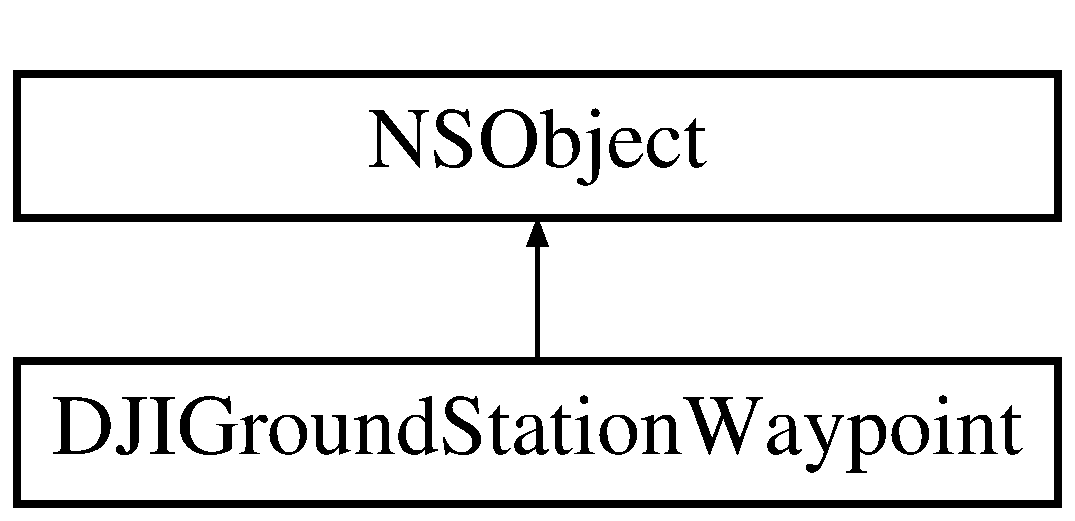
\includegraphics[height=2.000000cm]{interface_d_j_i_ground_station_waypoint}
\end{center}
\end{figure}
\subsection*{Instance Methods}
\begin{DoxyCompactItemize}
\item 
\hypertarget{interface_d_j_i_ground_station_waypoint_a40abddf2f95fb0d9a460ef288a3c2637}{(id) -\/ {\bfseries init\+With\+Coordinate\+:}}\label{interface_d_j_i_ground_station_waypoint_a40abddf2f95fb0d9a460ef288a3c2637}

\end{DoxyCompactItemize}
\subsection*{Properties}
\begin{DoxyCompactItemize}
\item 
C\+L\+Location\+Coordinate2\+D \hyperlink{interface_d_j_i_ground_station_waypoint_a40261f153c4a5cc55158cec8d45cfce1}{coordinate}
\item 
float \hyperlink{interface_d_j_i_ground_station_waypoint_a455e76a89605973616fcb7dd3f9944f9}{altitude}
\item 
float \hyperlink{interface_d_j_i_ground_station_waypoint_a173aad3e3662ad891f33015b1dc5e549}{horizontal\+Velocity}
\item 
int \hyperlink{interface_d_j_i_ground_station_waypoint_af492d8fd1160afec55ba567bc9d40f5a}{stay\+Time}
\end{DoxyCompactItemize}


\subsection{Property Documentation}
\hypertarget{interface_d_j_i_ground_station_waypoint_a455e76a89605973616fcb7dd3f9944f9}{\index{D\+J\+I\+Ground\+Station\+Waypoint@{D\+J\+I\+Ground\+Station\+Waypoint}!altitude@{altitude}}
\index{altitude@{altitude}!D\+J\+I\+Ground\+Station\+Waypoint@{D\+J\+I\+Ground\+Station\+Waypoint}}
\subsubsection[{altitude}]{\setlength{\rightskip}{0pt plus 5cm}-\/ (float) altitude\hspace{0.3cm}{\ttfamily [read]}, {\ttfamily [write]}, {\ttfamily [nonatomic]}, {\ttfamily [assign]}}}\label{interface_d_j_i_ground_station_waypoint_a455e76a89605973616fcb7dd3f9944f9}
Altitude (meters) \hypertarget{interface_d_j_i_ground_station_waypoint_a40261f153c4a5cc55158cec8d45cfce1}{\index{D\+J\+I\+Ground\+Station\+Waypoint@{D\+J\+I\+Ground\+Station\+Waypoint}!coordinate@{coordinate}}
\index{coordinate@{coordinate}!D\+J\+I\+Ground\+Station\+Waypoint@{D\+J\+I\+Ground\+Station\+Waypoint}}
\subsubsection[{coordinate}]{\setlength{\rightskip}{0pt plus 5cm}-\/ (C\+L\+Location\+Coordinate2\+D) coordinate\hspace{0.3cm}{\ttfamily [read]}, {\ttfamily [write]}, {\ttfamily [nonatomic]}, {\ttfamily [assign]}}}\label{interface_d_j_i_ground_station_waypoint_a40261f153c4a5cc55158cec8d45cfce1}
Waypoint coordinate (degree) \hypertarget{interface_d_j_i_ground_station_waypoint_a173aad3e3662ad891f33015b1dc5e549}{\index{D\+J\+I\+Ground\+Station\+Waypoint@{D\+J\+I\+Ground\+Station\+Waypoint}!horizontal\+Velocity@{horizontal\+Velocity}}
\index{horizontal\+Velocity@{horizontal\+Velocity}!D\+J\+I\+Ground\+Station\+Waypoint@{D\+J\+I\+Ground\+Station\+Waypoint}}
\subsubsection[{horizontal\+Velocity}]{\setlength{\rightskip}{0pt plus 5cm}-\/ (float) horizontal\+Velocity\hspace{0.3cm}{\ttfamily [read]}, {\ttfamily [write]}, {\ttfamily [nonatomic]}, {\ttfamily [assign]}}}\label{interface_d_j_i_ground_station_waypoint_a173aad3e3662ad891f33015b1dc5e549}
Horizontal velocity (m/s) \hypertarget{interface_d_j_i_ground_station_waypoint_af492d8fd1160afec55ba567bc9d40f5a}{\index{D\+J\+I\+Ground\+Station\+Waypoint@{D\+J\+I\+Ground\+Station\+Waypoint}!stay\+Time@{stay\+Time}}
\index{stay\+Time@{stay\+Time}!D\+J\+I\+Ground\+Station\+Waypoint@{D\+J\+I\+Ground\+Station\+Waypoint}}
\subsubsection[{stay\+Time}]{\setlength{\rightskip}{0pt plus 5cm}-\/ (int) stay\+Time\hspace{0.3cm}{\ttfamily [read]}, {\ttfamily [write]}, {\ttfamily [nonatomic]}, {\ttfamily [assign]}}}\label{interface_d_j_i_ground_station_waypoint_af492d8fd1160afec55ba567bc9d40f5a}
Staying time at waypoint (second) 

The documentation for this class was generated from the following file\+:\begin{DoxyCompactItemize}
\item 
D\+J\+I\+Ground\+Station\+Waypoint.\+h\end{DoxyCompactItemize}

\hypertarget{struct_d_j_i_limit_fly_status}{\section{D\+J\+I\+Limit\+Fly\+Status Struct Reference}
\label{struct_d_j_i_limit_fly_status}\index{D\+J\+I\+Limit\+Fly\+Status@{D\+J\+I\+Limit\+Fly\+Status}}
}
\subsection*{Protected Attributes}
\begin{DoxyCompactItemize}
\item 
\hypertarget{struct_d_j_i_limit_fly_status_a9a4cb948196626d43241b068f38d3d65}{B\+O\+O\+L {\bfseries is\+Reach\+Max\+Height}}\label{struct_d_j_i_limit_fly_status_a9a4cb948196626d43241b068f38d3d65}

\item 
\hypertarget{struct_d_j_i_limit_fly_status_a6b3b93eefacd0d511bcbbcdd4ecc8bb1}{B\+O\+O\+L {\bfseries is\+Reach\+Max\+Distance}}\label{struct_d_j_i_limit_fly_status_a6b3b93eefacd0d511bcbbcdd4ecc8bb1}

\item 
\hypertarget{struct_d_j_i_limit_fly_status_aa57d194d52e9f9230246e95cb4f45448}{Float32 {\bfseries max\+Limit\+Height}}\label{struct_d_j_i_limit_fly_status_aa57d194d52e9f9230246e95cb4f45448}

\item 
\hypertarget{struct_d_j_i_limit_fly_status_a9c3e913b5e425fcc81b0eb061ed4a041}{Float32 {\bfseries max\+Limit\+Distance}}\label{struct_d_j_i_limit_fly_status_a9c3e913b5e425fcc81b0eb061ed4a041}

\end{DoxyCompactItemize}


The documentation for this struct was generated from the following file\+:\begin{DoxyCompactItemize}
\item 
D\+J\+I\+Main\+Controller.\+h\end{DoxyCompactItemize}

\hypertarget{interface_d_j_i_main_controller}{\section{D\+J\+I\+Main\+Controller Class Reference}
\label{interface_d_j_i_main_controller}\index{D\+J\+I\+Main\+Controller@{D\+J\+I\+Main\+Controller}}
}
Inheritance diagram for D\+J\+I\+Main\+Controller\+:\begin{figure}[H]
\begin{center}
\leavevmode
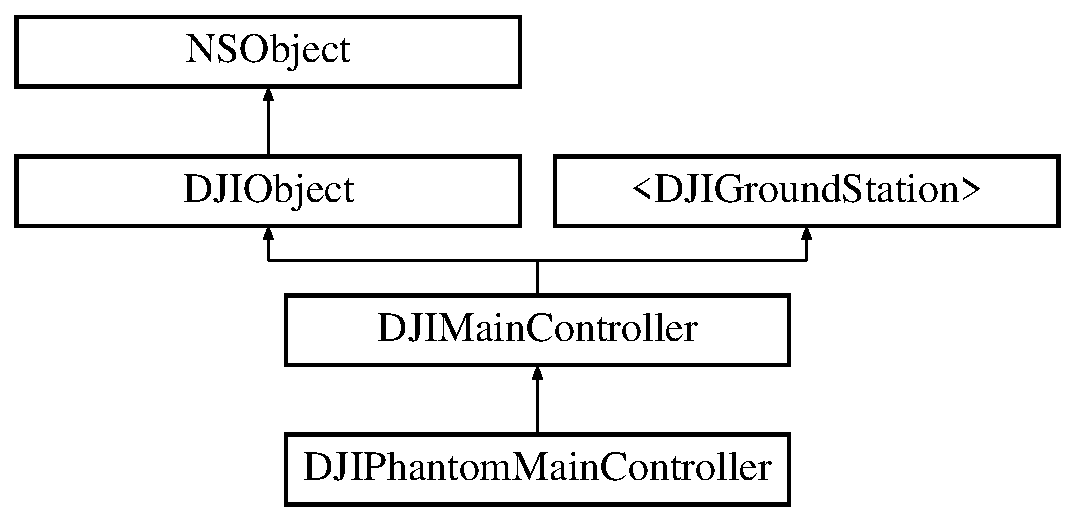
\includegraphics[height=4.000000cm]{interface_d_j_i_main_controller}
\end{center}
\end{figure}
\subsection*{Instance Methods}
\begin{DoxyCompactItemize}
\item 
(N\+S\+String $\ast$) -\/ \hyperlink{interface_d_j_i_main_controller_a405f7a49a8e7862464766a1e215a5c60}{get\+Main\+Controller\+Version}
\item 
(void) -\/ \hyperlink{interface_d_j_i_main_controller_a1879097a70fea7c2018ce2eb2083cafe}{start\+Update\+M\+C\+System\+State}
\item 
(void) -\/ \hyperlink{interface_d_j_i_main_controller_a23dd04927a580453afd2e688428ddabd}{stop\+Update\+M\+C\+System\+State}
\item 
(void) -\/ \hyperlink{interface_d_j_i_main_controller_a0eda335cc5b54d7427b2f34650da82a1}{set\+Limit\+Fly\+With\+Height\+:\+Distance\+:with\+Result\+:}
\item 
(void) -\/ \hyperlink{interface_d_j_i_main_controller_a41046d8038c97e2ae343d1df44eb5e3e}{get\+Limit\+Fly\+With\+Result\+Block\+:}
\item 
(void) -\/ \hyperlink{interface_d_j_i_main_controller_a98f618b316a5a302fe48d8592b95f5e4}{set\+No\+Fly\+:with\+Result\+:}
\item 
(void) -\/ \hyperlink{interface_d_j_i_main_controller_acb2e17e16ef2a7ed81a3a18e92ed2e88}{set\+Home\+Point\+:with\+Result\+:}
\item 
(void) -\/ \hyperlink{interface_d_j_i_main_controller_af4932ba75990e8c494e7f13b3a964c01}{get\+Home\+Point\+:}
\item 
(void) -\/ \hyperlink{interface_d_j_i_main_controller_adbea3d5c73fac755f88f82a16caf195f}{set\+Go\+Home\+Default\+Altitude\+:with\+Result\+:}
\item 
(void) -\/ \hyperlink{interface_d_j_i_main_controller_ae970b7f329da79a0aad189e339531d2b}{get\+Go\+Home\+Default\+Altitude\+:}
\item 
(void) -\/ \hyperlink{interface_d_j_i_main_controller_acf2c3e3ef4926bdbfcb1f7624f847b26}{set\+Go\+Home\+Temporary\+Altitude\+:with\+Result\+:}
\item 
(void) -\/ \hyperlink{interface_d_j_i_main_controller_a1f1d3ea5c7bd179f398484ff37207474}{get\+Go\+Home\+Temporary\+Altitude\+:}
\end{DoxyCompactItemize}
\subsection*{Properties}
\begin{DoxyCompactItemize}
\item 
id$<$ \hyperlink{protocol_d_j_i_main_controller_delegate-p}{D\+J\+I\+Main\+Controller\+Delegate} $>$ \hyperlink{interface_d_j_i_main_controller_a6ae013235289f0feaac2ca0ddda474b7}{mc\+Delegate}
\end{DoxyCompactItemize}


\subsection{Method Documentation}
\hypertarget{interface_d_j_i_main_controller_ae970b7f329da79a0aad189e339531d2b}{\index{D\+J\+I\+Main\+Controller@{D\+J\+I\+Main\+Controller}!get\+Go\+Home\+Default\+Altitude\+:@{get\+Go\+Home\+Default\+Altitude\+:}}
\index{get\+Go\+Home\+Default\+Altitude\+:@{get\+Go\+Home\+Default\+Altitude\+:}!D\+J\+I\+Main\+Controller@{D\+J\+I\+Main\+Controller}}
\subsubsection[{get\+Go\+Home\+Default\+Altitude\+:}]{\setlength{\rightskip}{0pt plus 5cm}-\/ (void) get\+Go\+Home\+Default\+Altitude\+: 
\begin{DoxyParamCaption}
\item[{(void($^\wedge$)(float altitude, {\bf D\+J\+I\+Error} $\ast$error))}]{block}
\end{DoxyParamCaption}
}}\label{interface_d_j_i_main_controller_ae970b7f329da79a0aad189e339531d2b}
Get the default altitude of go home.


\begin{DoxyParams}{Parameters}
{\em block} & Remote execute result \\
\hline
\end{DoxyParams}
\hypertarget{interface_d_j_i_main_controller_a1f1d3ea5c7bd179f398484ff37207474}{\index{D\+J\+I\+Main\+Controller@{D\+J\+I\+Main\+Controller}!get\+Go\+Home\+Temporary\+Altitude\+:@{get\+Go\+Home\+Temporary\+Altitude\+:}}
\index{get\+Go\+Home\+Temporary\+Altitude\+:@{get\+Go\+Home\+Temporary\+Altitude\+:}!D\+J\+I\+Main\+Controller@{D\+J\+I\+Main\+Controller}}
\subsubsection[{get\+Go\+Home\+Temporary\+Altitude\+:}]{\setlength{\rightskip}{0pt plus 5cm}-\/ (void) get\+Go\+Home\+Temporary\+Altitude\+: 
\begin{DoxyParamCaption}
\item[{(void($^\wedge$)(float altitude, {\bf D\+J\+I\+Error} $\ast$error))}]{block}
\end{DoxyParamCaption}
}}\label{interface_d_j_i_main_controller_a1f1d3ea5c7bd179f398484ff37207474}
Get go home default altitude.


\begin{DoxyParams}{Parameters}
{\em block} & Remote execute result \\
\hline
\end{DoxyParams}
\hypertarget{interface_d_j_i_main_controller_af4932ba75990e8c494e7f13b3a964c01}{\index{D\+J\+I\+Main\+Controller@{D\+J\+I\+Main\+Controller}!get\+Home\+Point\+:@{get\+Home\+Point\+:}}
\index{get\+Home\+Point\+:@{get\+Home\+Point\+:}!D\+J\+I\+Main\+Controller@{D\+J\+I\+Main\+Controller}}
\subsubsection[{get\+Home\+Point\+:}]{\setlength{\rightskip}{0pt plus 5cm}-\/ (void) get\+Home\+Point\+: 
\begin{DoxyParamCaption}
\item[{(void($^\wedge$)(C\+L\+Location\+Coordinate2\+D home\+Point, {\bf D\+J\+I\+Error} $\ast$error))}]{block}
\end{DoxyParamCaption}
}}\label{interface_d_j_i_main_controller_af4932ba75990e8c494e7f13b3a964c01}
Get home point of drone.


\begin{DoxyParams}{Parameters}
{\em block} & Remote execute result. The home\+Point is in degree. \\
\hline
\end{DoxyParams}
\hypertarget{interface_d_j_i_main_controller_a41046d8038c97e2ae343d1df44eb5e3e}{\index{D\+J\+I\+Main\+Controller@{D\+J\+I\+Main\+Controller}!get\+Limit\+Fly\+With\+Result\+Block\+:@{get\+Limit\+Fly\+With\+Result\+Block\+:}}
\index{get\+Limit\+Fly\+With\+Result\+Block\+:@{get\+Limit\+Fly\+With\+Result\+Block\+:}!D\+J\+I\+Main\+Controller@{D\+J\+I\+Main\+Controller}}
\subsubsection[{get\+Limit\+Fly\+With\+Result\+Block\+:}]{\setlength{\rightskip}{0pt plus 5cm}-\/ (void) get\+Limit\+Fly\+With\+Result\+Block\+: 
\begin{DoxyParamCaption}
\item[{(void($^\wedge$)({\bf D\+J\+I\+Limit\+Fly\+Status} limit\+Status, {\bf D\+J\+I\+Error} $\ast$))}]{block}
\end{DoxyParamCaption}
}}\label{interface_d_j_i_main_controller_a41046d8038c97e2ae343d1df44eb5e3e}
Get the limit fly parameter. if execute success, result will be set to 'limit\+Fly\+Parameter'


\begin{DoxyParams}{Parameters}
{\em block} & Remote execute result \\
\hline
\end{DoxyParams}
\hypertarget{interface_d_j_i_main_controller_a405f7a49a8e7862464766a1e215a5c60}{\index{D\+J\+I\+Main\+Controller@{D\+J\+I\+Main\+Controller}!get\+Main\+Controller\+Version@{get\+Main\+Controller\+Version}}
\index{get\+Main\+Controller\+Version@{get\+Main\+Controller\+Version}!D\+J\+I\+Main\+Controller@{D\+J\+I\+Main\+Controller}}
\subsubsection[{get\+Main\+Controller\+Version}]{\setlength{\rightskip}{0pt plus 5cm}-\/ (N\+S\+String$\ast$) get\+Main\+Controller\+Version 
\begin{DoxyParamCaption}
{}
\end{DoxyParamCaption}
}}\label{interface_d_j_i_main_controller_a405f7a49a8e7862464766a1e215a5c60}
Main controller's firmware version. \hypertarget{interface_d_j_i_main_controller_adbea3d5c73fac755f88f82a16caf195f}{\index{D\+J\+I\+Main\+Controller@{D\+J\+I\+Main\+Controller}!set\+Go\+Home\+Default\+Altitude\+:with\+Result\+:@{set\+Go\+Home\+Default\+Altitude\+:with\+Result\+:}}
\index{set\+Go\+Home\+Default\+Altitude\+:with\+Result\+:@{set\+Go\+Home\+Default\+Altitude\+:with\+Result\+:}!D\+J\+I\+Main\+Controller@{D\+J\+I\+Main\+Controller}}
\subsubsection[{set\+Go\+Home\+Default\+Altitude\+:with\+Result\+:}]{\setlength{\rightskip}{0pt plus 5cm}-\/ (void) set\+Go\+Home\+Default\+Altitude\+: 
\begin{DoxyParamCaption}
\item[{(float)}]{altitude}
\item[{withResult:(D\+J\+I\+Execute\+Result\+Block)}]{block}
\end{DoxyParamCaption}
}}\label{interface_d_j_i_main_controller_adbea3d5c73fac755f88f82a16caf195f}
Set go home default altitude. The default altitude is used by the drone every time while going home.


\begin{DoxyParams}{Parameters}
{\em altitude} & Drone altitude in meter for going home. \mbox{[}20m -\/ 500m\mbox{]} and could not over the limited height. \\
\hline
{\em block} & Remote execute result \\
\hline
\end{DoxyParams}
\hypertarget{interface_d_j_i_main_controller_acf2c3e3ef4926bdbfcb1f7624f847b26}{\index{D\+J\+I\+Main\+Controller@{D\+J\+I\+Main\+Controller}!set\+Go\+Home\+Temporary\+Altitude\+:with\+Result\+:@{set\+Go\+Home\+Temporary\+Altitude\+:with\+Result\+:}}
\index{set\+Go\+Home\+Temporary\+Altitude\+:with\+Result\+:@{set\+Go\+Home\+Temporary\+Altitude\+:with\+Result\+:}!D\+J\+I\+Main\+Controller@{D\+J\+I\+Main\+Controller}}
\subsubsection[{set\+Go\+Home\+Temporary\+Altitude\+:with\+Result\+:}]{\setlength{\rightskip}{0pt plus 5cm}-\/ (void) set\+Go\+Home\+Temporary\+Altitude\+: 
\begin{DoxyParamCaption}
\item[{(float)}]{tmp\+Altitude}
\item[{withResult:(D\+J\+I\+Execute\+Result\+Block)}]{block}
\end{DoxyParamCaption}
}}\label{interface_d_j_i_main_controller_acf2c3e3ef4926bdbfcb1f7624f847b26}
Set go home temporary altitude. The temporary altitude is used by the drone this time while going home.


\begin{DoxyParams}{Parameters}
{\em tmp\+Altitude} & Drone temporary altitude in meter for going home. \mbox{[}20m -\/ 500m\mbox{]} and could not over the limited height. \\
\hline
{\em block} & Remote execute result \\
\hline
\end{DoxyParams}
\hypertarget{interface_d_j_i_main_controller_acb2e17e16ef2a7ed81a3a18e92ed2e88}{\index{D\+J\+I\+Main\+Controller@{D\+J\+I\+Main\+Controller}!set\+Home\+Point\+:with\+Result\+:@{set\+Home\+Point\+:with\+Result\+:}}
\index{set\+Home\+Point\+:with\+Result\+:@{set\+Home\+Point\+:with\+Result\+:}!D\+J\+I\+Main\+Controller@{D\+J\+I\+Main\+Controller}}
\subsubsection[{set\+Home\+Point\+:with\+Result\+:}]{\setlength{\rightskip}{0pt plus 5cm}-\/ (void) set\+Home\+Point\+: 
\begin{DoxyParamCaption}
\item[{(C\+L\+Location\+Coordinate2\+D)}]{home\+Point}
\item[{withResult:(D\+J\+I\+Execute\+Result\+Block)}]{block}
\end{DoxyParamCaption}
}}\label{interface_d_j_i_main_controller_acb2e17e16ef2a7ed81a3a18e92ed2e88}
Set home point to drone. Home point is use for back home when the drone lost signal or other case. The drone use current located location as default home point while it first start and receive enough satellite( $>$= 6). User should be carefully to change the home point.


\begin{DoxyParams}{Parameters}
{\em home\+Point} & Home point in degree. \\
\hline
{\em block} & Remote execute result \\
\hline
\end{DoxyParams}
\hypertarget{interface_d_j_i_main_controller_a0eda335cc5b54d7427b2f34650da82a1}{\index{D\+J\+I\+Main\+Controller@{D\+J\+I\+Main\+Controller}!set\+Limit\+Fly\+With\+Height\+:\+Distance\+:with\+Result\+:@{set\+Limit\+Fly\+With\+Height\+:\+Distance\+:with\+Result\+:}}
\index{set\+Limit\+Fly\+With\+Height\+:\+Distance\+:with\+Result\+:@{set\+Limit\+Fly\+With\+Height\+:\+Distance\+:with\+Result\+:}!D\+J\+I\+Main\+Controller@{D\+J\+I\+Main\+Controller}}
\subsubsection[{set\+Limit\+Fly\+With\+Height\+:\+Distance\+:with\+Result\+:}]{\setlength{\rightskip}{0pt plus 5cm}-\/ (void) set\+Limit\+Fly\+With\+Height\+: 
\begin{DoxyParamCaption}
\item[{(float)}]{height}
\item[{Distance:(float)}]{distance}
\item[{withResult:(D\+J\+I\+Execute\+Result\+Block)}]{block}
\end{DoxyParamCaption}
}}\label{interface_d_j_i_main_controller_a0eda335cc5b54d7427b2f34650da82a1}
Set the fly limitation parameter.


\begin{DoxyParams}{Parameters}
{\em limit\+Param} & The max height and distance parameters \\
\hline
{\em block} & Remote execute result \\
\hline
\end{DoxyParams}
\hypertarget{interface_d_j_i_main_controller_a98f618b316a5a302fe48d8592b95f5e4}{\index{D\+J\+I\+Main\+Controller@{D\+J\+I\+Main\+Controller}!set\+No\+Fly\+:with\+Result\+:@{set\+No\+Fly\+:with\+Result\+:}}
\index{set\+No\+Fly\+:with\+Result\+:@{set\+No\+Fly\+:with\+Result\+:}!D\+J\+I\+Main\+Controller@{D\+J\+I\+Main\+Controller}}
\subsubsection[{set\+No\+Fly\+:with\+Result\+:}]{\setlength{\rightskip}{0pt plus 5cm}-\/ (void) set\+No\+Fly\+: 
\begin{DoxyParamCaption}
\item[{({\bf D\+J\+I\+No\+Fly\+Zone})}]{no\+Fly\+Zone}
\item[{withResult:(D\+J\+I\+Execute\+Result\+Block)}]{block}
\end{DoxyParamCaption}
}}\label{interface_d_j_i_main_controller_a98f618b316a5a302fe48d8592b95f5e4}
Set a no fly zone. Not support now.


\begin{DoxyParams}{Parameters}
{\em no\+Fly\+Zone} & No fly zone parameter \\
\hline
{\em block} & Remote execute result \\
\hline
\end{DoxyParams}
\hypertarget{interface_d_j_i_main_controller_a1879097a70fea7c2018ce2eb2083cafe}{\index{D\+J\+I\+Main\+Controller@{D\+J\+I\+Main\+Controller}!start\+Update\+M\+C\+System\+State@{start\+Update\+M\+C\+System\+State}}
\index{start\+Update\+M\+C\+System\+State@{start\+Update\+M\+C\+System\+State}!D\+J\+I\+Main\+Controller@{D\+J\+I\+Main\+Controller}}
\subsubsection[{start\+Update\+M\+C\+System\+State}]{\setlength{\rightskip}{0pt plus 5cm}-\/ (void) start\+Update\+M\+C\+System\+State 
\begin{DoxyParamCaption}
{}
\end{DoxyParamCaption}
}}\label{interface_d_j_i_main_controller_a1879097a70fea7c2018ce2eb2083cafe}
Start update main controller's system state \hypertarget{interface_d_j_i_main_controller_a23dd04927a580453afd2e688428ddabd}{\index{D\+J\+I\+Main\+Controller@{D\+J\+I\+Main\+Controller}!stop\+Update\+M\+C\+System\+State@{stop\+Update\+M\+C\+System\+State}}
\index{stop\+Update\+M\+C\+System\+State@{stop\+Update\+M\+C\+System\+State}!D\+J\+I\+Main\+Controller@{D\+J\+I\+Main\+Controller}}
\subsubsection[{stop\+Update\+M\+C\+System\+State}]{\setlength{\rightskip}{0pt plus 5cm}-\/ (void) stop\+Update\+M\+C\+System\+State 
\begin{DoxyParamCaption}
{}
\end{DoxyParamCaption}
}}\label{interface_d_j_i_main_controller_a23dd04927a580453afd2e688428ddabd}
Stop update main controller's system state 

\subsection{Property Documentation}
\hypertarget{interface_d_j_i_main_controller_a6ae013235289f0feaac2ca0ddda474b7}{\index{D\+J\+I\+Main\+Controller@{D\+J\+I\+Main\+Controller}!mc\+Delegate@{mc\+Delegate}}
\index{mc\+Delegate@{mc\+Delegate}!D\+J\+I\+Main\+Controller@{D\+J\+I\+Main\+Controller}}
\subsubsection[{mc\+Delegate}]{\setlength{\rightskip}{0pt plus 5cm}-\/ (id$<${\bf D\+J\+I\+Main\+Controller\+Delegate}$>$) mc\+Delegate\hspace{0.3cm}{\ttfamily [read]}, {\ttfamily [write]}, {\ttfamily [nonatomic]}, {\ttfamily [weak]}}}\label{interface_d_j_i_main_controller_a6ae013235289f0feaac2ca0ddda474b7}
Manin controller delegate 

The documentation for this class was generated from the following file\+:\begin{DoxyCompactItemize}
\item 
D\+J\+I\+Main\+Controller.\+h\end{DoxyCompactItemize}

\hypertarget{protocol_d_j_i_main_controller_delegate-p}{\section{$<$D\+J\+I\+Main\+Controller\+Delegate$>$ Protocol Reference}
\label{protocol_d_j_i_main_controller_delegate-p}\index{$<$\+D\+J\+I\+Main\+Controller\+Delegate$>$@{$<$\+D\+J\+I\+Main\+Controller\+Delegate$>$}}
}
Inheritance diagram for $<$D\+J\+I\+Main\+Controller\+Delegate$>$\+:\begin{figure}[H]
\begin{center}
\leavevmode
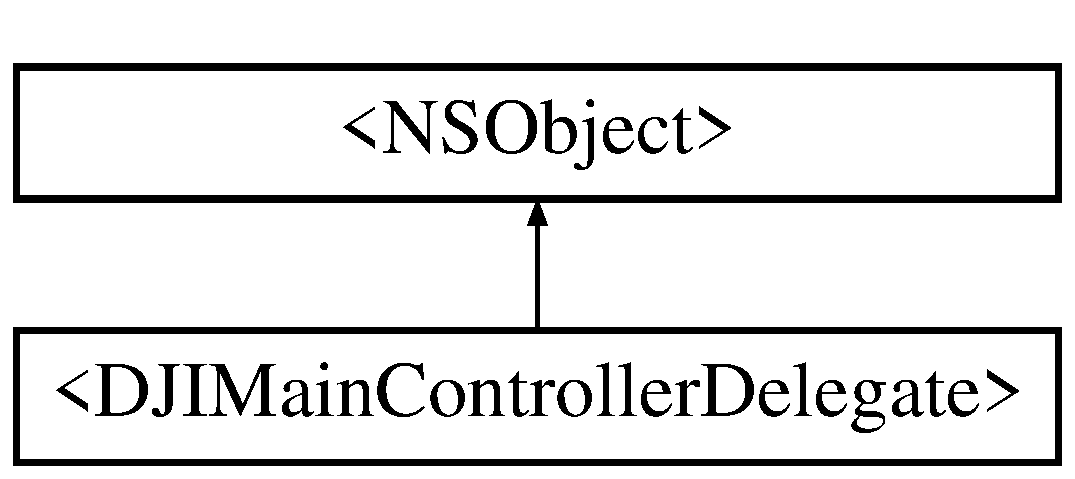
\includegraphics[height=2.000000cm]{protocol_d_j_i_main_controller_delegate-p}
\end{center}
\end{figure}
\subsection*{Instance Methods}
\begin{DoxyCompactItemize}
\item 
(void) -\/ \hyperlink{protocol_d_j_i_main_controller_delegate-p_acbb11b8d37bbcf49fa6763921de3c77c}{main\+Controller\+:did\+Main\+Control\+Error\+:}
\item 
(void) -\/ \hyperlink{protocol_d_j_i_main_controller_delegate-p_ae9d64c21b32e83fa8e7b4e04f01f9d98}{main\+Controller\+:did\+Update\+System\+State\+:}
\end{DoxyCompactItemize}


\subsection{Method Documentation}
\hypertarget{protocol_d_j_i_main_controller_delegate-p_acbb11b8d37bbcf49fa6763921de3c77c}{\index{D\+J\+I\+Main\+Controller\+Delegate-\/p@{D\+J\+I\+Main\+Controller\+Delegate-\/p}!main\+Controller\+:did\+Main\+Control\+Error\+:@{main\+Controller\+:did\+Main\+Control\+Error\+:}}
\index{main\+Controller\+:did\+Main\+Control\+Error\+:@{main\+Controller\+:did\+Main\+Control\+Error\+:}!D\+J\+I\+Main\+Controller\+Delegate-\/p@{D\+J\+I\+Main\+Controller\+Delegate-\/p}}
\subsubsection[{main\+Controller\+:did\+Main\+Control\+Error\+:}]{\setlength{\rightskip}{0pt plus 5cm}-\/ (void) main\+Controller\+: 
\begin{DoxyParamCaption}
\item[{({\bf D\+J\+I\+Main\+Controller} $\ast$)}]{mc}
\item[{didMainControlError:(M\+C\+Error)}]{error}
\end{DoxyParamCaption}
\hspace{0.3cm}{\ttfamily [optional]}}}\label{protocol_d_j_i_main_controller_delegate-p_acbb11b8d37bbcf49fa6763921de3c77c}
Notify on main controller error \hypertarget{protocol_d_j_i_main_controller_delegate-p_ae9d64c21b32e83fa8e7b4e04f01f9d98}{\index{D\+J\+I\+Main\+Controller\+Delegate-\/p@{D\+J\+I\+Main\+Controller\+Delegate-\/p}!main\+Controller\+:did\+Update\+System\+State\+:@{main\+Controller\+:did\+Update\+System\+State\+:}}
\index{main\+Controller\+:did\+Update\+System\+State\+:@{main\+Controller\+:did\+Update\+System\+State\+:}!D\+J\+I\+Main\+Controller\+Delegate-\/p@{D\+J\+I\+Main\+Controller\+Delegate-\/p}}
\subsubsection[{main\+Controller\+:did\+Update\+System\+State\+:}]{\setlength{\rightskip}{0pt plus 5cm}-\/ (void) main\+Controller\+: 
\begin{DoxyParamCaption}
\item[{({\bf D\+J\+I\+Main\+Controller} $\ast$)}]{mc}
\item[{didUpdateSystemState:({\bf D\+J\+I\+M\+C\+System\+State} $\ast$)}]{state}
\end{DoxyParamCaption}
\hspace{0.3cm}{\ttfamily [optional]}}}\label{protocol_d_j_i_main_controller_delegate-p_ae9d64c21b32e83fa8e7b4e04f01f9d98}
Update main controller system state 

The documentation for this protocol was generated from the following file\+:\begin{DoxyCompactItemize}
\item 
D\+J\+I\+Main\+Controller.\+h\end{DoxyCompactItemize}

\hypertarget{interface_d_j_i_m_c_smart_go_home_data}{\section{D\+J\+I\+M\+C\+Smart\+Go\+Home\+Data Class Reference}
\label{interface_d_j_i_m_c_smart_go_home_data}\index{D\+J\+I\+M\+C\+Smart\+Go\+Home\+Data@{D\+J\+I\+M\+C\+Smart\+Go\+Home\+Data}}
}
Inheritance diagram for D\+J\+I\+M\+C\+Smart\+Go\+Home\+Data\+:\begin{figure}[H]
\begin{center}
\leavevmode
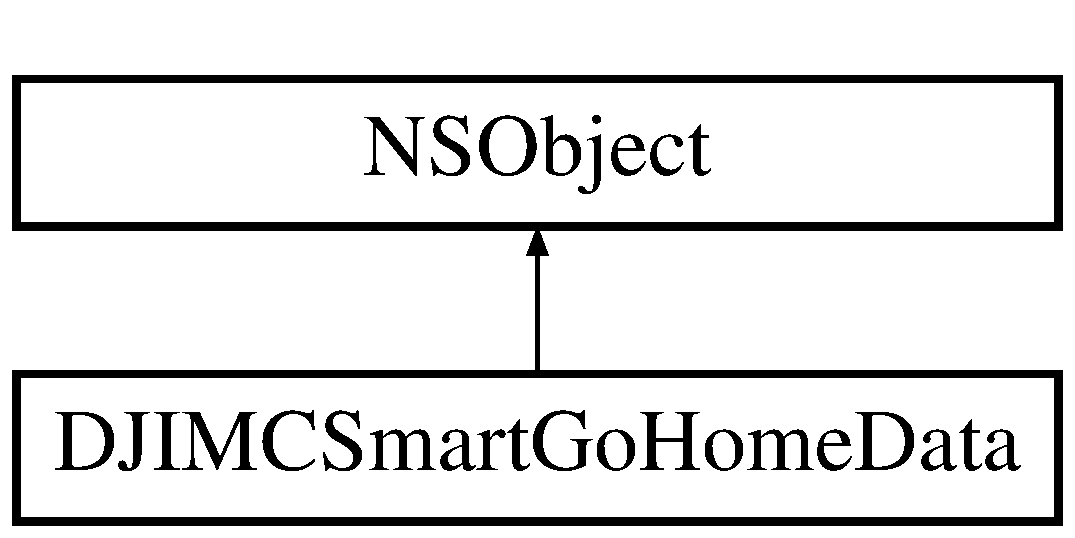
\includegraphics[height=2.000000cm]{interface_d_j_i_m_c_smart_go_home_data}
\end{center}
\end{figure}
\subsection*{Properties}
\begin{DoxyCompactItemize}
\item 
\hypertarget{interface_d_j_i_m_c_smart_go_home_data_ac1b8d2714eb85f9c38c216ada484f7d8}{N\+S\+U\+Integer {\bfseries remain\+Time\+For\+Flight}}\label{interface_d_j_i_m_c_smart_go_home_data_ac1b8d2714eb85f9c38c216ada484f7d8}

\item 
\hypertarget{interface_d_j_i_m_c_smart_go_home_data_a5704e59eb614cde4296b2127c1fcb210}{N\+S\+U\+Integer {\bfseries time\+For\+Go\+Home}}\label{interface_d_j_i_m_c_smart_go_home_data_a5704e59eb614cde4296b2127c1fcb210}

\item 
\hypertarget{interface_d_j_i_m_c_smart_go_home_data_ae280122e70f4f1168dd02f237b468260}{N\+S\+U\+Integer {\bfseries time\+For\+Landing}}\label{interface_d_j_i_m_c_smart_go_home_data_ae280122e70f4f1168dd02f237b468260}

\item 
\hypertarget{interface_d_j_i_m_c_smart_go_home_data_a8e9fbbdecd3912100d1d9a38b8fc0023}{N\+S\+U\+Integer {\bfseries power\+Percent\+For\+Go\+Home}}\label{interface_d_j_i_m_c_smart_go_home_data_a8e9fbbdecd3912100d1d9a38b8fc0023}

\item 
\hypertarget{interface_d_j_i_m_c_smart_go_home_data_a7f95c8777ba25ceb9e9522ab25f02188}{N\+S\+U\+Integer {\bfseries power\+Percent\+For\+Landing}}\label{interface_d_j_i_m_c_smart_go_home_data_a7f95c8777ba25ceb9e9522ab25f02188}

\item 
\hypertarget{interface_d_j_i_m_c_smart_go_home_data_ae513310a32691fc240fe3722b266c03d}{float {\bfseries radius\+For\+Go\+Home}}\label{interface_d_j_i_m_c_smart_go_home_data_ae513310a32691fc240fe3722b266c03d}

\item 
\hypertarget{interface_d_j_i_m_c_smart_go_home_data_aa37f6b80c036ff0d5bbdbe01928c7726}{B\+O\+O\+L {\bfseries drone\+Request\+Go\+Home}}\label{interface_d_j_i_m_c_smart_go_home_data_aa37f6b80c036ff0d5bbdbe01928c7726}

\end{DoxyCompactItemize}


The documentation for this class was generated from the following file\+:\begin{DoxyCompactItemize}
\item 
D\+J\+I\+M\+C\+Smart\+Go\+Home.\+h\end{DoxyCompactItemize}

\hypertarget{interface_d_j_i_m_c_system_state}{\section{D\+J\+I\+M\+C\+System\+State Class Reference}
\label{interface_d_j_i_m_c_system_state}\index{D\+J\+I\+M\+C\+System\+State@{D\+J\+I\+M\+C\+System\+State}}
}
Inheritance diagram for D\+J\+I\+M\+C\+System\+State\+:\begin{figure}[H]
\begin{center}
\leavevmode
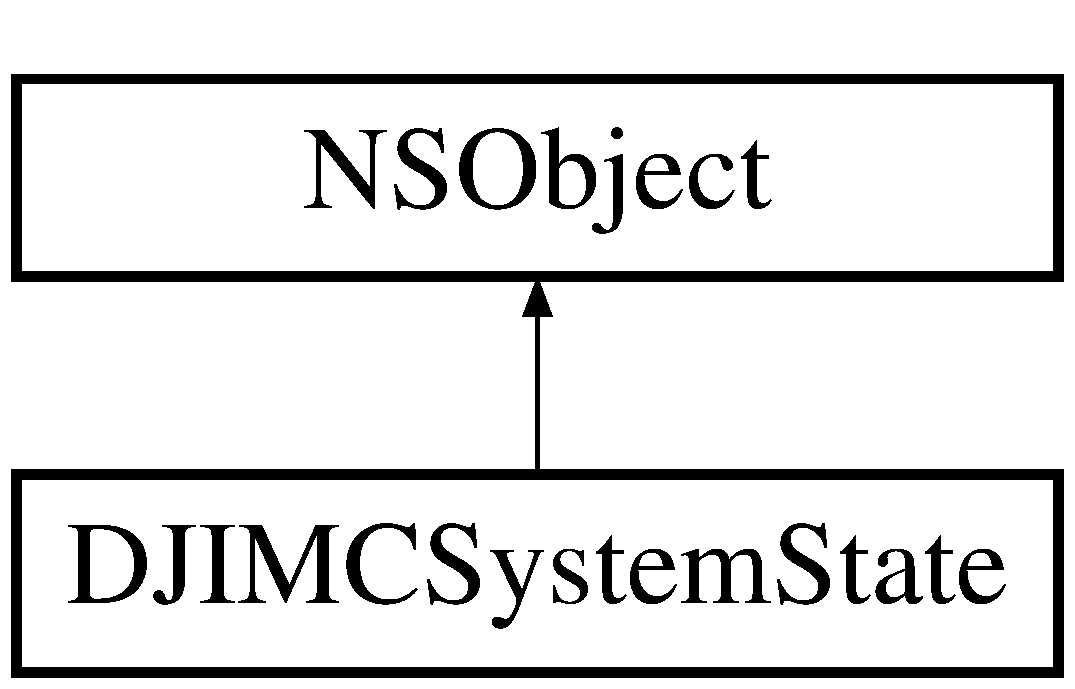
\includegraphics[height=2.000000cm]{interface_d_j_i_m_c_system_state}
\end{center}
\end{figure}
\subsection*{Properties}
\begin{DoxyCompactItemize}
\item 
int \hyperlink{interface_d_j_i_m_c_system_state_a1d8684af50d70620b9166d2c6a469f63}{satellite\+Count}
\item 
C\+L\+Location\+Coordinate2\+D \hyperlink{interface_d_j_i_m_c_system_state_a4395f4e24d0f084407cf99fdf4d630b2}{home\+Location}
\item 
C\+L\+Location\+Coordinate2\+D \hyperlink{interface_d_j_i_m_c_system_state_a90f991829772ba3e7bb23811845fb2cc}{drone\+Location}
\item 
float \hyperlink{interface_d_j_i_m_c_system_state_a325798d4e0c80ec568fdf36ce1098901}{velocity\+X}
\item 
float \hyperlink{interface_d_j_i_m_c_system_state_aa41385209d9edaef3f4d6ee6385b471b}{velocity\+Y}
\item 
float \hyperlink{interface_d_j_i_m_c_system_state_ab2bee010d83187db9a3ded5456494e8a}{velocity\+Z}
\item 
float \hyperlink{interface_d_j_i_m_c_system_state_a14fa4428eae3c3c96789a44d41d0a8d8}{altitude}
\item 
\hyperlink{struct_d_j_i_attitude}{D\+J\+I\+Attitude} \hyperlink{interface_d_j_i_m_c_system_state_af6916800ba242ddaa3ede17625224021}{attitude}
\item 
int \hyperlink{interface_d_j_i_m_c_system_state_ab39cb3387140f0642d29d865ba33e166}{power\+Level}
\item 
B\+O\+O\+L \hyperlink{interface_d_j_i_m_c_system_state_a7d0f82dcfa7ba2650c394815a0ce9e06}{is\+Flying}
\item 
D\+J\+I\+Main\+Controller\+Flight\+Mode \hyperlink{interface_d_j_i_m_c_system_state_a7ecc5f31a38b34a94f6680f7fc6f590c}{flight\+Mode}
\item 
D\+J\+I\+Main\+Controller\+No\+Fly\+Status \hyperlink{interface_d_j_i_m_c_system_state_ab1d284a6e00a0fed3c262e69d3b738ab}{no\+Fly\+Status}
\item 
C\+L\+Location\+Coordinate2\+D \hyperlink{interface_d_j_i_m_c_system_state_a1840e97a45fe5f712af878e9aec09e0d}{no\+Fly\+Zone\+Center}
\item 
int \hyperlink{interface_d_j_i_m_c_system_state_a79b5f1ed799acf989c4c755523df582a}{no\+Fly\+Zone\+Radius}
\item 
\hyperlink{interface_d_j_i_m_c_smart_go_home_data}{D\+J\+I\+M\+C\+Smart\+Go\+Home\+Data} $\ast$ \hyperlink{interface_d_j_i_m_c_system_state_a66a05759183d6c6bd20b309f274c189a}{smart\+Go\+Home\+Data}
\end{DoxyCompactItemize}


\subsection{Property Documentation}
\hypertarget{interface_d_j_i_m_c_system_state_a14fa4428eae3c3c96789a44d41d0a8d8}{\index{D\+J\+I\+M\+C\+System\+State@{D\+J\+I\+M\+C\+System\+State}!altitude@{altitude}}
\index{altitude@{altitude}!D\+J\+I\+M\+C\+System\+State@{D\+J\+I\+M\+C\+System\+State}}
\subsubsection[{altitude}]{\setlength{\rightskip}{0pt plus 5cm}-\/ (float) altitude\hspace{0.3cm}{\ttfamily [read]}, {\ttfamily [nonatomic]}, {\ttfamily [assign]}}}\label{interface_d_j_i_m_c_system_state_a14fa4428eae3c3c96789a44d41d0a8d8}
Altitude of the drone, (0.\+1m) \hypertarget{interface_d_j_i_m_c_system_state_af6916800ba242ddaa3ede17625224021}{\index{D\+J\+I\+M\+C\+System\+State@{D\+J\+I\+M\+C\+System\+State}!attitude@{attitude}}
\index{attitude@{attitude}!D\+J\+I\+M\+C\+System\+State@{D\+J\+I\+M\+C\+System\+State}}
\subsubsection[{attitude}]{\setlength{\rightskip}{0pt plus 5cm}-\/ ({\bf D\+J\+I\+Attitude}) attitude\hspace{0.3cm}{\ttfamily [read]}, {\ttfamily [nonatomic]}, {\ttfamily [assign]}}}\label{interface_d_j_i_m_c_system_state_af6916800ba242ddaa3ede17625224021}
Attitude of the drone, Pitch\mbox{[}-\/180, 180\mbox{]}, Roll\mbox{[}-\/180, 180\mbox{]}, Yaw\mbox{[}-\/180, 180\mbox{]} \hypertarget{interface_d_j_i_m_c_system_state_a90f991829772ba3e7bb23811845fb2cc}{\index{D\+J\+I\+M\+C\+System\+State@{D\+J\+I\+M\+C\+System\+State}!drone\+Location@{drone\+Location}}
\index{drone\+Location@{drone\+Location}!D\+J\+I\+M\+C\+System\+State@{D\+J\+I\+M\+C\+System\+State}}
\subsubsection[{drone\+Location}]{\setlength{\rightskip}{0pt plus 5cm}-\/ (C\+L\+Location\+Coordinate2\+D) drone\+Location\hspace{0.3cm}{\ttfamily [read]}, {\ttfamily [nonatomic]}, {\ttfamily [assign]}}}\label{interface_d_j_i_m_c_system_state_a90f991829772ba3e7bb23811845fb2cc}
Current location of the drone \hypertarget{interface_d_j_i_m_c_system_state_a7ecc5f31a38b34a94f6680f7fc6f590c}{\index{D\+J\+I\+M\+C\+System\+State@{D\+J\+I\+M\+C\+System\+State}!flight\+Mode@{flight\+Mode}}
\index{flight\+Mode@{flight\+Mode}!D\+J\+I\+M\+C\+System\+State@{D\+J\+I\+M\+C\+System\+State}}
\subsubsection[{flight\+Mode}]{\setlength{\rightskip}{0pt plus 5cm}-\/ (D\+J\+I\+Main\+Controller\+Flight\+Mode) flight\+Mode\hspace{0.3cm}{\ttfamily [read]}, {\ttfamily [nonatomic]}, {\ttfamily [assign]}}}\label{interface_d_j_i_m_c_system_state_a7ecc5f31a38b34a94f6680f7fc6f590c}
Flight mode \hypertarget{interface_d_j_i_m_c_system_state_a4395f4e24d0f084407cf99fdf4d630b2}{\index{D\+J\+I\+M\+C\+System\+State@{D\+J\+I\+M\+C\+System\+State}!home\+Location@{home\+Location}}
\index{home\+Location@{home\+Location}!D\+J\+I\+M\+C\+System\+State@{D\+J\+I\+M\+C\+System\+State}}
\subsubsection[{home\+Location}]{\setlength{\rightskip}{0pt plus 5cm}-\/ (C\+L\+Location\+Coordinate2\+D) home\+Location\hspace{0.3cm}{\ttfamily [read]}, {\ttfamily [nonatomic]}, {\ttfamily [assign]}}}\label{interface_d_j_i_m_c_system_state_a4395f4e24d0f084407cf99fdf4d630b2}
Home location of the drone \hypertarget{interface_d_j_i_m_c_system_state_a7d0f82dcfa7ba2650c394815a0ce9e06}{\index{D\+J\+I\+M\+C\+System\+State@{D\+J\+I\+M\+C\+System\+State}!is\+Flying@{is\+Flying}}
\index{is\+Flying@{is\+Flying}!D\+J\+I\+M\+C\+System\+State@{D\+J\+I\+M\+C\+System\+State}}
\subsubsection[{is\+Flying}]{\setlength{\rightskip}{0pt plus 5cm}-\/ (B\+O\+O\+L) is\+Flying\hspace{0.3cm}{\ttfamily [read]}, {\ttfamily [nonatomic]}, {\ttfamily [assign]}}}\label{interface_d_j_i_m_c_system_state_a7d0f82dcfa7ba2650c394815a0ce9e06}
Whether the drone is in flying \hypertarget{interface_d_j_i_m_c_system_state_ab1d284a6e00a0fed3c262e69d3b738ab}{\index{D\+J\+I\+M\+C\+System\+State@{D\+J\+I\+M\+C\+System\+State}!no\+Fly\+Status@{no\+Fly\+Status}}
\index{no\+Fly\+Status@{no\+Fly\+Status}!D\+J\+I\+M\+C\+System\+State@{D\+J\+I\+M\+C\+System\+State}}
\subsubsection[{no\+Fly\+Status}]{\setlength{\rightskip}{0pt plus 5cm}-\/ (D\+J\+I\+Main\+Controller\+No\+Fly\+Status) no\+Fly\+Status\hspace{0.3cm}{\ttfamily [read]}, {\ttfamily [nonatomic]}, {\ttfamily [assign]}}}\label{interface_d_j_i_m_c_system_state_ab1d284a6e00a0fed3c262e69d3b738ab}
No fly status \hypertarget{interface_d_j_i_m_c_system_state_a1840e97a45fe5f712af878e9aec09e0d}{\index{D\+J\+I\+M\+C\+System\+State@{D\+J\+I\+M\+C\+System\+State}!no\+Fly\+Zone\+Center@{no\+Fly\+Zone\+Center}}
\index{no\+Fly\+Zone\+Center@{no\+Fly\+Zone\+Center}!D\+J\+I\+M\+C\+System\+State@{D\+J\+I\+M\+C\+System\+State}}
\subsubsection[{no\+Fly\+Zone\+Center}]{\setlength{\rightskip}{0pt plus 5cm}-\/ (C\+L\+Location\+Coordinate2\+D) no\+Fly\+Zone\+Center\hspace{0.3cm}{\ttfamily [read]}, {\ttfamily [nonatomic]}, {\ttfamily [assign]}}}\label{interface_d_j_i_m_c_system_state_a1840e97a45fe5f712af878e9aec09e0d}
The no fly zone center coordinate \hypertarget{interface_d_j_i_m_c_system_state_a79b5f1ed799acf989c4c755523df582a}{\index{D\+J\+I\+M\+C\+System\+State@{D\+J\+I\+M\+C\+System\+State}!no\+Fly\+Zone\+Radius@{no\+Fly\+Zone\+Radius}}
\index{no\+Fly\+Zone\+Radius@{no\+Fly\+Zone\+Radius}!D\+J\+I\+M\+C\+System\+State@{D\+J\+I\+M\+C\+System\+State}}
\subsubsection[{no\+Fly\+Zone\+Radius}]{\setlength{\rightskip}{0pt plus 5cm}-\/ (int) no\+Fly\+Zone\+Radius\hspace{0.3cm}{\ttfamily [read]}, {\ttfamily [nonatomic]}, {\ttfamily [assign]}}}\label{interface_d_j_i_m_c_system_state_a79b5f1ed799acf989c4c755523df582a}
The no fly zone radius \hypertarget{interface_d_j_i_m_c_system_state_ab39cb3387140f0642d29d865ba33e166}{\index{D\+J\+I\+M\+C\+System\+State@{D\+J\+I\+M\+C\+System\+State}!power\+Level@{power\+Level}}
\index{power\+Level@{power\+Level}!D\+J\+I\+M\+C\+System\+State@{D\+J\+I\+M\+C\+System\+State}}
\subsubsection[{power\+Level}]{\setlength{\rightskip}{0pt plus 5cm}-\/ (int) power\+Level\hspace{0.3cm}{\ttfamily [read]}, {\ttfamily [nonatomic]}, {\ttfamily [assign]}}}\label{interface_d_j_i_m_c_system_state_ab39cb3387140f0642d29d865ba33e166}
Power level of the drone\+: 0 -\/ very low power warning, 1-\/ low power warning, 2 -\/ height power, 3 -\/ full power \hypertarget{interface_d_j_i_m_c_system_state_a1d8684af50d70620b9166d2c6a469f63}{\index{D\+J\+I\+M\+C\+System\+State@{D\+J\+I\+M\+C\+System\+State}!satellite\+Count@{satellite\+Count}}
\index{satellite\+Count@{satellite\+Count}!D\+J\+I\+M\+C\+System\+State@{D\+J\+I\+M\+C\+System\+State}}
\subsubsection[{satellite\+Count}]{\setlength{\rightskip}{0pt plus 5cm}-\/ (int) satellite\+Count\hspace{0.3cm}{\ttfamily [read]}, {\ttfamily [nonatomic]}, {\ttfamily [assign]}}}\label{interface_d_j_i_m_c_system_state_a1d8684af50d70620b9166d2c6a469f63}
Satellite count. \hypertarget{interface_d_j_i_m_c_system_state_a66a05759183d6c6bd20b309f274c189a}{\index{D\+J\+I\+M\+C\+System\+State@{D\+J\+I\+M\+C\+System\+State}!smart\+Go\+Home\+Data@{smart\+Go\+Home\+Data}}
\index{smart\+Go\+Home\+Data@{smart\+Go\+Home\+Data}!D\+J\+I\+M\+C\+System\+State@{D\+J\+I\+M\+C\+System\+State}}
\subsubsection[{smart\+Go\+Home\+Data}]{\setlength{\rightskip}{0pt plus 5cm}-\/ ({\bf D\+J\+I\+M\+C\+Smart\+Go\+Home\+Data}$\ast$) smart\+Go\+Home\+Data\hspace{0.3cm}{\ttfamily [read]}, {\ttfamily [nonatomic]}, {\ttfamily [assign]}}}\label{interface_d_j_i_m_c_system_state_a66a05759183d6c6bd20b309f274c189a}
Smart go home data \hypertarget{interface_d_j_i_m_c_system_state_a325798d4e0c80ec568fdf36ce1098901}{\index{D\+J\+I\+M\+C\+System\+State@{D\+J\+I\+M\+C\+System\+State}!velocity\+X@{velocity\+X}}
\index{velocity\+X@{velocity\+X}!D\+J\+I\+M\+C\+System\+State@{D\+J\+I\+M\+C\+System\+State}}
\subsubsection[{velocity\+X}]{\setlength{\rightskip}{0pt plus 5cm}-\/ (float) velocity\+X\hspace{0.3cm}{\ttfamily [read]}, {\ttfamily [nonatomic]}, {\ttfamily [assign]}}}\label{interface_d_j_i_m_c_system_state_a325798d4e0c80ec568fdf36ce1098901}
Speed x (m/s) \hypertarget{interface_d_j_i_m_c_system_state_aa41385209d9edaef3f4d6ee6385b471b}{\index{D\+J\+I\+M\+C\+System\+State@{D\+J\+I\+M\+C\+System\+State}!velocity\+Y@{velocity\+Y}}
\index{velocity\+Y@{velocity\+Y}!D\+J\+I\+M\+C\+System\+State@{D\+J\+I\+M\+C\+System\+State}}
\subsubsection[{velocity\+Y}]{\setlength{\rightskip}{0pt plus 5cm}-\/ (float) velocity\+Y\hspace{0.3cm}{\ttfamily [read]}, {\ttfamily [nonatomic]}, {\ttfamily [assign]}}}\label{interface_d_j_i_m_c_system_state_aa41385209d9edaef3f4d6ee6385b471b}
Speed y (m/s) \hypertarget{interface_d_j_i_m_c_system_state_ab2bee010d83187db9a3ded5456494e8a}{\index{D\+J\+I\+M\+C\+System\+State@{D\+J\+I\+M\+C\+System\+State}!velocity\+Z@{velocity\+Z}}
\index{velocity\+Z@{velocity\+Z}!D\+J\+I\+M\+C\+System\+State@{D\+J\+I\+M\+C\+System\+State}}
\subsubsection[{velocity\+Z}]{\setlength{\rightskip}{0pt plus 5cm}-\/ (float) velocity\+Z\hspace{0.3cm}{\ttfamily [read]}, {\ttfamily [nonatomic]}, {\ttfamily [assign]}}}\label{interface_d_j_i_m_c_system_state_ab2bee010d83187db9a3ded5456494e8a}
Speed z (m/s) 

The documentation for this class was generated from the following file\+:\begin{DoxyCompactItemize}
\item 
D\+J\+I\+M\+C\+System\+State.\+h\end{DoxyCompactItemize}

\hypertarget{interface_d_j_i_media}{\section{D\+J\+I\+Media Class Reference}
\label{interface_d_j_i_media}\index{D\+J\+I\+Media@{D\+J\+I\+Media}}
}
Inheritance diagram for D\+J\+I\+Media\+:\begin{figure}[H]
\begin{center}
\leavevmode
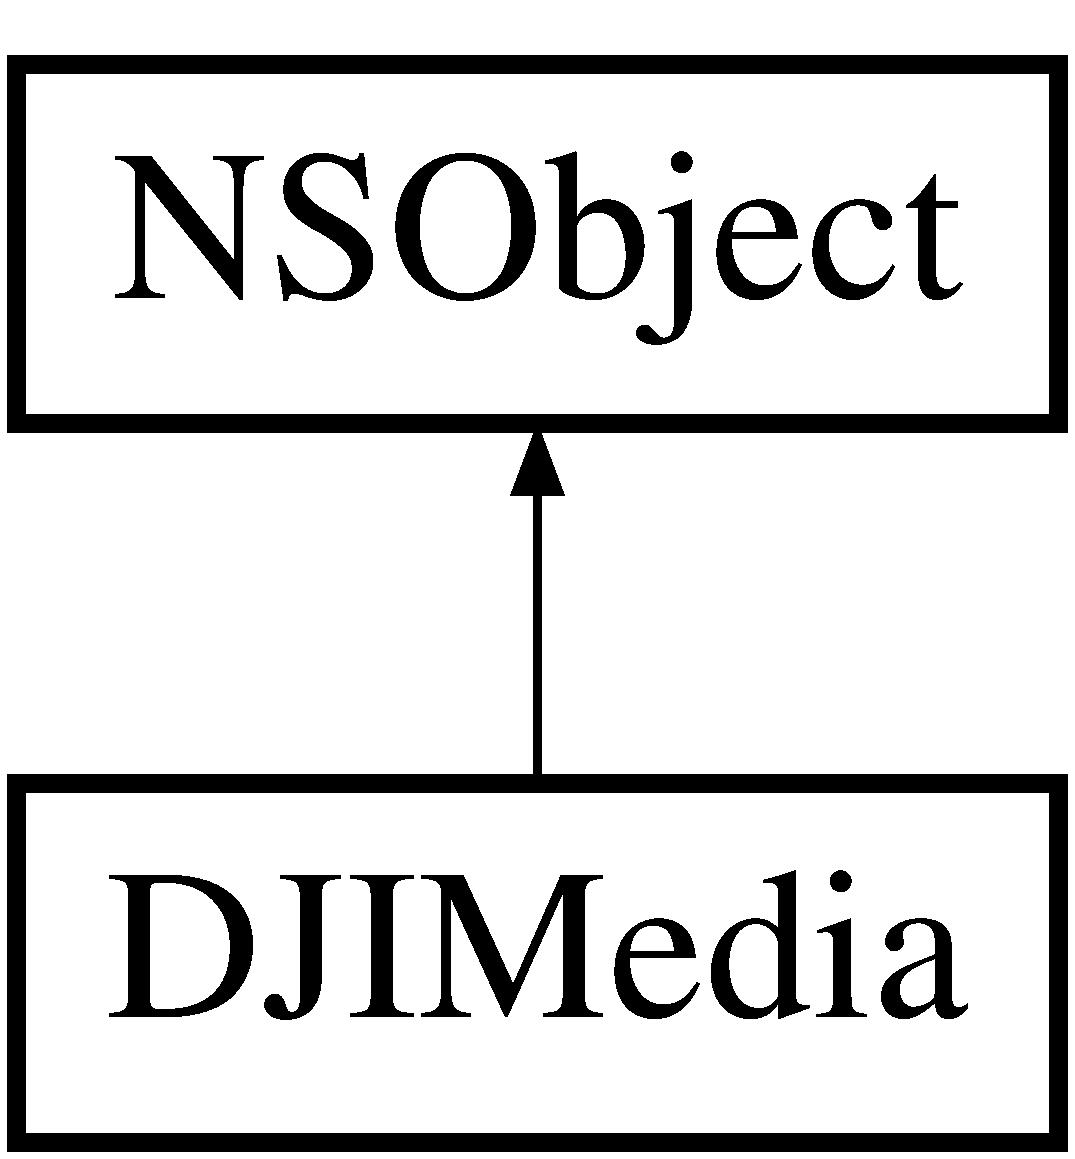
\includegraphics[height=2.000000cm]{interface_d_j_i_media}
\end{center}
\end{figure}
\subsection*{Instance Methods}
\begin{DoxyCompactItemize}
\item 
\hypertarget{interface_d_j_i_media_af280a622a09271b06b9c095d1a8e2a63}{(id) -\/ {\bfseries init\+With\+Media\+U\+R\+L\+:}}\label{interface_d_j_i_media_af280a622a09271b06b9c095d1a8e2a63}

\item 
(void) -\/ \hyperlink{interface_d_j_i_media_a00d41d73d3223136633c46edfaa13f7c}{fetch\+Thumbnail\+:}
\item 
(void) -\/ \hyperlink{interface_d_j_i_media_a843d3c6122be27f15d3c0c8c4119962e}{fetch\+Media\+Data\+:}
\end{DoxyCompactItemize}
\subsection*{Protected Attributes}
\begin{DoxyCompactItemize}
\item 
\hypertarget{interface_d_j_i_media_ac6087ab0b801da8df2f4be91a35a2b09}{D\+J\+I\+Media\+Context $\ast$ {\bfseries \+\_\+media\+Context}}\label{interface_d_j_i_media_ac6087ab0b801da8df2f4be91a35a2b09}

\end{DoxyCompactItemize}
\subsection*{Properties}
\begin{DoxyCompactItemize}
\item 
\hypertarget{interface_d_j_i_media_a9e45dd2c5999cb51ea28d27589074ec4}{D\+J\+I\+Media\+Context $\ast$ {\bfseries media\+Context}}\label{interface_d_j_i_media_a9e45dd2c5999cb51ea28d27589074ec4}

\item 
N\+S\+String $\ast$ \hyperlink{interface_d_j_i_media_ad57506b4b8d11c702f55ce934b243fd4}{file\+Name}
\item 
long long \hyperlink{interface_d_j_i_media_aad9cace96d93c6d5cb0a09cc88683ce7}{file\+Size}
\item 
N\+S\+String $\ast$ \hyperlink{interface_d_j_i_media_a5fca68c2fabc5e5f2b10ca028ad68954}{create\+Time}
\item 
float \hyperlink{interface_d_j_i_media_a530c5cebcd1ffa67e1b32e73946f3961}{duration\+Seconds}
\item 
Media\+Type \hyperlink{interface_d_j_i_media_a72e5f802cc23493a1105001685c592dd}{media\+Type}
\item 
N\+S\+String $\ast$ \hyperlink{interface_d_j_i_media_ab7c862faf6304e43f5f1ce49762e1b0d}{media\+U\+R\+L}
\item 
U\+I\+Image $\ast$ \hyperlink{interface_d_j_i_media_ab3f581d4ba9f69844becf18ebfeb6d2c}{thumbnail}
\end{DoxyCompactItemize}


\subsection{Method Documentation}
\hypertarget{interface_d_j_i_media_a843d3c6122be27f15d3c0c8c4119962e}{\index{D\+J\+I\+Media@{D\+J\+I\+Media}!fetch\+Media\+Data\+:@{fetch\+Media\+Data\+:}}
\index{fetch\+Media\+Data\+:@{fetch\+Media\+Data\+:}!D\+J\+I\+Media@{D\+J\+I\+Media}}
\subsubsection[{fetch\+Media\+Data\+:}]{\setlength{\rightskip}{0pt plus 5cm}-\/ (void) fetch\+Media\+Data\+: 
\begin{DoxyParamCaption}
\item[{(Async\+Fetch\+Handler)}]{handler}
\end{DoxyParamCaption}
}}\label{interface_d_j_i_media_a843d3c6122be27f15d3c0c8c4119962e}
Fetch media data from remote media


\begin{DoxyParams}{Parameters}
{\em handler} & async handler data when received data frome remote \\
\hline
\end{DoxyParams}
\hypertarget{interface_d_j_i_media_a00d41d73d3223136633c46edfaa13f7c}{\index{D\+J\+I\+Media@{D\+J\+I\+Media}!fetch\+Thumbnail\+:@{fetch\+Thumbnail\+:}}
\index{fetch\+Thumbnail\+:@{fetch\+Thumbnail\+:}!D\+J\+I\+Media@{D\+J\+I\+Media}}
\subsubsection[{fetch\+Thumbnail\+:}]{\setlength{\rightskip}{0pt plus 5cm}-\/ (void) fetch\+Thumbnail\+: 
\begin{DoxyParamCaption}
\item[{(Async\+Operation\+Handler)}]{completion}
\end{DoxyParamCaption}
}}\label{interface_d_j_i_media_a00d41d73d3223136633c46edfaa13f7c}
Fetch thumbnail from remote media


\begin{DoxyParams}{Parameters}
{\em completion} & if there is no error, property \char`\"{}thumbnail\char`\"{} will be set \\
\hline
\end{DoxyParams}


\subsection{Property Documentation}
\hypertarget{interface_d_j_i_media_a5fca68c2fabc5e5f2b10ca028ad68954}{\index{D\+J\+I\+Media@{D\+J\+I\+Media}!create\+Time@{create\+Time}}
\index{create\+Time@{create\+Time}!D\+J\+I\+Media@{D\+J\+I\+Media}}
\subsubsection[{create\+Time}]{\setlength{\rightskip}{0pt plus 5cm}-\/ (N\+S\+String$\ast$) create\+Time\hspace{0.3cm}{\ttfamily [read]}, {\ttfamily [nonatomic]}, {\ttfamily [assign]}}}\label{interface_d_j_i_media_a5fca68c2fabc5e5f2b10ca028ad68954}
The media's create time \hypertarget{interface_d_j_i_media_a530c5cebcd1ffa67e1b32e73946f3961}{\index{D\+J\+I\+Media@{D\+J\+I\+Media}!duration\+Seconds@{duration\+Seconds}}
\index{duration\+Seconds@{duration\+Seconds}!D\+J\+I\+Media@{D\+J\+I\+Media}}
\subsubsection[{duration\+Seconds}]{\setlength{\rightskip}{0pt plus 5cm}-\/ (float) duration\+Seconds\hspace{0.3cm}{\ttfamily [read]}, {\ttfamily [nonatomic]}, {\ttfamily [assign]}}}\label{interface_d_j_i_media_a530c5cebcd1ffa67e1b32e73946f3961}
If media is video. this property is show the duration of the video \hypertarget{interface_d_j_i_media_ad57506b4b8d11c702f55ce934b243fd4}{\index{D\+J\+I\+Media@{D\+J\+I\+Media}!file\+Name@{file\+Name}}
\index{file\+Name@{file\+Name}!D\+J\+I\+Media@{D\+J\+I\+Media}}
\subsubsection[{file\+Name}]{\setlength{\rightskip}{0pt plus 5cm}-\/ (N\+S\+String$\ast$) file\+Name\hspace{0.3cm}{\ttfamily [read]}, {\ttfamily [nonatomic]}, {\ttfamily [assign]}}}\label{interface_d_j_i_media_ad57506b4b8d11c702f55ce934b243fd4}
The media file name \hypertarget{interface_d_j_i_media_aad9cace96d93c6d5cb0a09cc88683ce7}{\index{D\+J\+I\+Media@{D\+J\+I\+Media}!file\+Size@{file\+Size}}
\index{file\+Size@{file\+Size}!D\+J\+I\+Media@{D\+J\+I\+Media}}
\subsubsection[{file\+Size}]{\setlength{\rightskip}{0pt plus 5cm}-\/ (long long) file\+Size\hspace{0.3cm}{\ttfamily [read]}, {\ttfamily [nonatomic]}, {\ttfamily [assign]}}}\label{interface_d_j_i_media_aad9cace96d93c6d5cb0a09cc88683ce7}
The media file size \hypertarget{interface_d_j_i_media_a72e5f802cc23493a1105001685c592dd}{\index{D\+J\+I\+Media@{D\+J\+I\+Media}!media\+Type@{media\+Type}}
\index{media\+Type@{media\+Type}!D\+J\+I\+Media@{D\+J\+I\+Media}}
\subsubsection[{media\+Type}]{\setlength{\rightskip}{0pt plus 5cm}-\/ (Media\+Type) media\+Type\hspace{0.3cm}{\ttfamily [read]}, {\ttfamily [nonatomic]}, {\ttfamily [assign]}}}\label{interface_d_j_i_media_a72e5f802cc23493a1105001685c592dd}
The media type \hypertarget{interface_d_j_i_media_ab7c862faf6304e43f5f1ce49762e1b0d}{\index{D\+J\+I\+Media@{D\+J\+I\+Media}!media\+U\+R\+L@{media\+U\+R\+L}}
\index{media\+U\+R\+L@{media\+U\+R\+L}!D\+J\+I\+Media@{D\+J\+I\+Media}}
\subsubsection[{media\+U\+R\+L}]{\setlength{\rightskip}{0pt plus 5cm}-\/ (N\+S\+String$\ast$) media\+U\+R\+L\hspace{0.3cm}{\ttfamily [read]}, {\ttfamily [nonatomic]}, {\ttfamily [assign]}}}\label{interface_d_j_i_media_ab7c862faf6304e43f5f1ce49762e1b0d}
The media url \hypertarget{interface_d_j_i_media_ab3f581d4ba9f69844becf18ebfeb6d2c}{\index{D\+J\+I\+Media@{D\+J\+I\+Media}!thumbnail@{thumbnail}}
\index{thumbnail@{thumbnail}!D\+J\+I\+Media@{D\+J\+I\+Media}}
\subsubsection[{thumbnail}]{\setlength{\rightskip}{0pt plus 5cm}-\/ (U\+I\+Image$\ast$) thumbnail\hspace{0.3cm}{\ttfamily [read]}, {\ttfamily [nonatomic]}, {\ttfamily [assign]}}}\label{interface_d_j_i_media_ab3f581d4ba9f69844becf18ebfeb6d2c}
Thumbnail image 

The documentation for this class was generated from the following file\+:\begin{DoxyCompactItemize}
\item 
D\+J\+I\+Media.\+h\end{DoxyCompactItemize}

\hypertarget{struct_d_j_i_no_fly_zone}{\section{D\+J\+I\+No\+Fly\+Zone Struct Reference}
\label{struct_d_j_i_no_fly_zone}\index{D\+J\+I\+No\+Fly\+Zone@{D\+J\+I\+No\+Fly\+Zone}}
}
\subsection*{Protected Attributes}
\begin{DoxyCompactItemize}
\item 
\hypertarget{struct_d_j_i_no_fly_zone_a835cc06cf44d2ec55ea722620e3a6a3e}{float {\bfseries zone\+Radius}}\label{struct_d_j_i_no_fly_zone_a835cc06cf44d2ec55ea722620e3a6a3e}

\item 
\hypertarget{struct_d_j_i_no_fly_zone_ac4dc5a958fa296e208d4d03a2a11f7b4}{C\+L\+Location\+Coordinate2\+D {\bfseries zone\+Center\+Coordinate}}\label{struct_d_j_i_no_fly_zone_ac4dc5a958fa296e208d4d03a2a11f7b4}

\end{DoxyCompactItemize}


The documentation for this struct was generated from the following file\+:\begin{DoxyCompactItemize}
\item 
D\+J\+I\+Main\+Controller.\+h\end{DoxyCompactItemize}

\hypertarget{interface_d_j_i_object}{\section{D\+J\+I\+Object Class Reference}
\label{interface_d_j_i_object}\index{D\+J\+I\+Object@{D\+J\+I\+Object}}
}
Inheritance diagram for D\+J\+I\+Object\+:\begin{figure}[H]
\begin{center}
\leavevmode
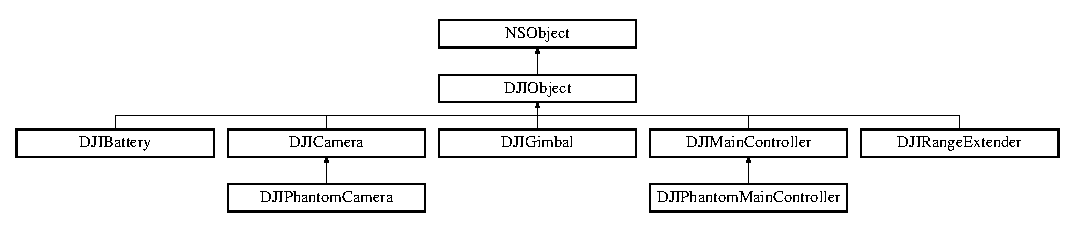
\includegraphics[height=2.619883cm]{interface_d_j_i_object}
\end{center}
\end{figure}


The documentation for this class was generated from the following file\+:\begin{DoxyCompactItemize}
\item 
D\+J\+I\+Object.\+h\end{DoxyCompactItemize}

\hypertarget{interface_d_j_i_phantom_camera}{\section{D\+J\+I\+Phantom\+Camera Class Reference}
\label{interface_d_j_i_phantom_camera}\index{D\+J\+I\+Phantom\+Camera@{D\+J\+I\+Phantom\+Camera}}
}
Inheritance diagram for D\+J\+I\+Phantom\+Camera\+:\begin{figure}[H]
\begin{center}
\leavevmode
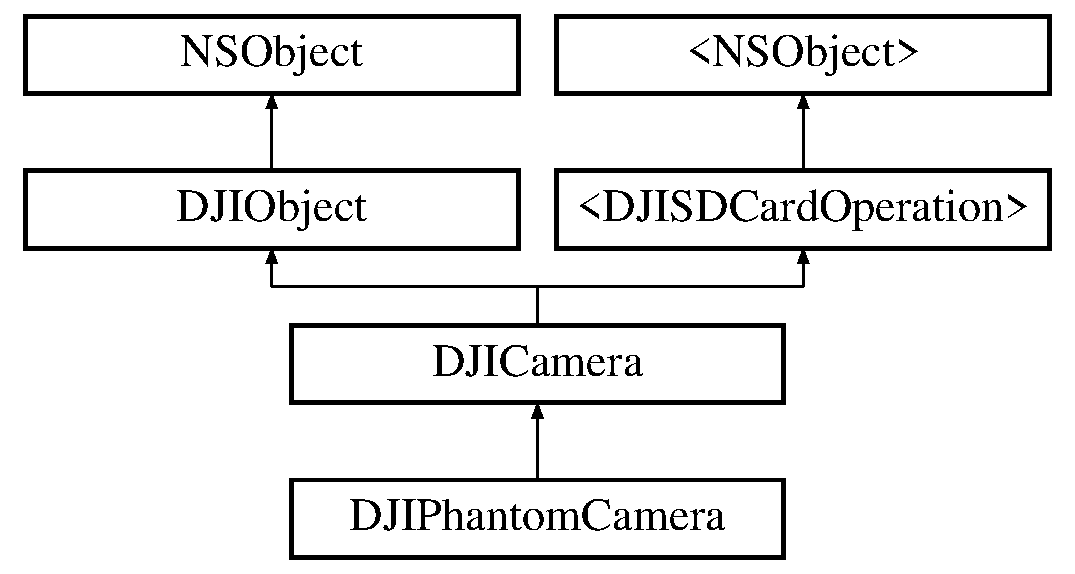
\includegraphics[height=4.000000cm]{interface_d_j_i_phantom_camera}
\end{center}
\end{figure}
\subsection*{Additional Inherited Members}


The documentation for this class was generated from the following file\+:\begin{DoxyCompactItemize}
\item 
D\+J\+I\+Phantom\+Camera.\+h\end{DoxyCompactItemize}

\hypertarget{interface_d_j_i_phantom_main_controller}{\section{D\+J\+I\+Phantom\+Main\+Controller Class Reference}
\label{interface_d_j_i_phantom_main_controller}\index{D\+J\+I\+Phantom\+Main\+Controller@{D\+J\+I\+Phantom\+Main\+Controller}}
}
Inheritance diagram for D\+J\+I\+Phantom\+Main\+Controller\+:\begin{figure}[H]
\begin{center}
\leavevmode
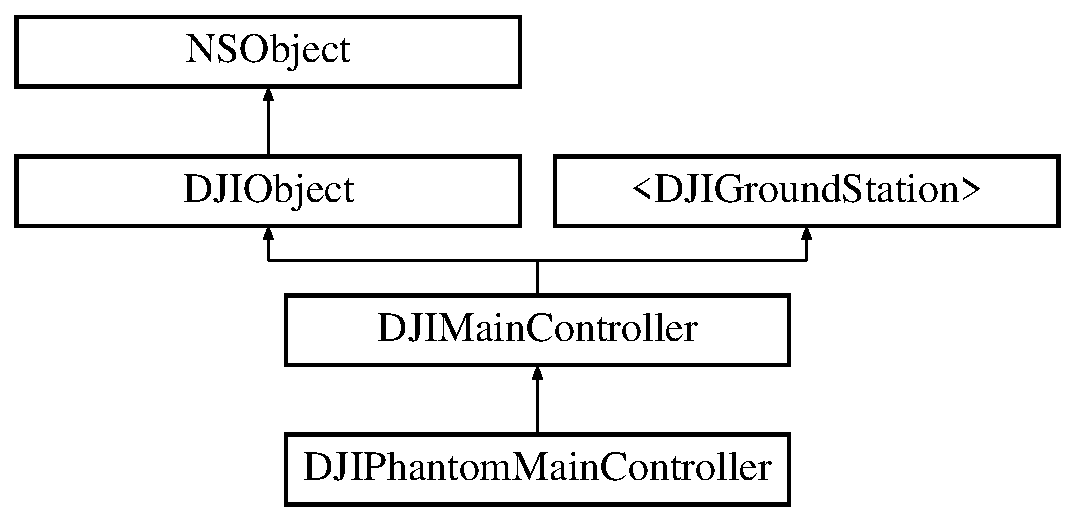
\includegraphics[height=4.000000cm]{interface_d_j_i_phantom_main_controller}
\end{center}
\end{figure}
\subsection*{Instance Methods}
\begin{DoxyCompactItemize}
\item 
(void) -\/ \hyperlink{interface_d_j_i_phantom_main_controller_ab0cb06ebdfd70108ca5e0835137007ac}{get\+M\+C\+System\+Mode\+:}
\item 
(void) -\/ \hyperlink{interface_d_j_i_phantom_main_controller_a051413e716f7d0540bfed22e35ad5686}{set\+Smart\+Go\+Home\+Enable\+:with\+Result\+:}
\item 
(void) -\/ \hyperlink{interface_d_j_i_phantom_main_controller_a6532d0d30d987cb5abfb710dbc7bf94c}{get\+Smart\+Go\+Home\+Enable\+:}
\item 
(void) -\/ \hyperlink{interface_d_j_i_phantom_main_controller_a4ac75d4b4381430bc9ff55d8a8466b2b}{confirm\+Go\+Home\+Reuqest\+:}
\item 
(void) -\/ \hyperlink{interface_d_j_i_phantom_main_controller_ae1edbf81ec14bc6e89420b0b6139e7ba}{ignore\+Go\+Home\+Reuqest\+:}
\end{DoxyCompactItemize}
\subsection*{Additional Inherited Members}


\subsection{Method Documentation}
\hypertarget{interface_d_j_i_phantom_main_controller_a4ac75d4b4381430bc9ff55d8a8466b2b}{\index{D\+J\+I\+Phantom\+Main\+Controller@{D\+J\+I\+Phantom\+Main\+Controller}!confirm\+Go\+Home\+Reuqest\+:@{confirm\+Go\+Home\+Reuqest\+:}}
\index{confirm\+Go\+Home\+Reuqest\+:@{confirm\+Go\+Home\+Reuqest\+:}!D\+J\+I\+Phantom\+Main\+Controller@{D\+J\+I\+Phantom\+Main\+Controller}}
\subsubsection[{confirm\+Go\+Home\+Reuqest\+:}]{\setlength{\rightskip}{0pt plus 5cm}-\/ (void) confirm\+Go\+Home\+Reuqest\+: 
\begin{DoxyParamCaption}
\item[{(D\+J\+I\+Execute\+Result\+Block)}]{block}
\end{DoxyParamCaption}
}}\label{interface_d_j_i_phantom_main_controller_a4ac75d4b4381430bc9ff55d8a8466b2b}
Confirm go home request. use to confirm go home request while the D\+J\+I\+M\+C\+Smart\+Go\+Home's drone\+Request\+Go\+Home is set.


\begin{DoxyParams}{Parameters}
{\em block} & Remote execute result \\
\hline
\end{DoxyParams}
\hypertarget{interface_d_j_i_phantom_main_controller_ab0cb06ebdfd70108ca5e0835137007ac}{\index{D\+J\+I\+Phantom\+Main\+Controller@{D\+J\+I\+Phantom\+Main\+Controller}!get\+M\+C\+System\+Mode\+:@{get\+M\+C\+System\+Mode\+:}}
\index{get\+M\+C\+System\+Mode\+:@{get\+M\+C\+System\+Mode\+:}!D\+J\+I\+Phantom\+Main\+Controller@{D\+J\+I\+Phantom\+Main\+Controller}}
\subsubsection[{get\+M\+C\+System\+Mode\+:}]{\setlength{\rightskip}{0pt plus 5cm}-\/ (void) get\+M\+C\+System\+Mode\+: 
\begin{DoxyParamCaption}
\item[{(void($^\wedge$)(D\+J\+I\+M\+C\+System\+Mode mode, {\bf D\+J\+I\+Error} $\ast$error))}]{block}
\end{DoxyParamCaption}
}}\label{interface_d_j_i_phantom_main_controller_ab0cb06ebdfd70108ca5e0835137007ac}
Get main controller's system mode.


\begin{DoxyParams}{Parameters}
{\em block} & Remote execute result \\
\hline
\end{DoxyParams}
\hypertarget{interface_d_j_i_phantom_main_controller_a6532d0d30d987cb5abfb710dbc7bf94c}{\index{D\+J\+I\+Phantom\+Main\+Controller@{D\+J\+I\+Phantom\+Main\+Controller}!get\+Smart\+Go\+Home\+Enable\+:@{get\+Smart\+Go\+Home\+Enable\+:}}
\index{get\+Smart\+Go\+Home\+Enable\+:@{get\+Smart\+Go\+Home\+Enable\+:}!D\+J\+I\+Phantom\+Main\+Controller@{D\+J\+I\+Phantom\+Main\+Controller}}
\subsubsection[{get\+Smart\+Go\+Home\+Enable\+:}]{\setlength{\rightskip}{0pt plus 5cm}-\/ (void) get\+Smart\+Go\+Home\+Enable\+: 
\begin{DoxyParamCaption}
\item[{(void($^\wedge$)(B\+O\+O\+L is\+Enable, {\bf D\+J\+I\+Error} $\ast$error))}]{block}
\end{DoxyParamCaption}
}}\label{interface_d_j_i_phantom_main_controller_a6532d0d30d987cb5abfb710dbc7bf94c}
Get smart go home enable.


\begin{DoxyParams}{Parameters}
{\em block} & Remote execute result \\
\hline
\end{DoxyParams}
\hypertarget{interface_d_j_i_phantom_main_controller_ae1edbf81ec14bc6e89420b0b6139e7ba}{\index{D\+J\+I\+Phantom\+Main\+Controller@{D\+J\+I\+Phantom\+Main\+Controller}!ignore\+Go\+Home\+Reuqest\+:@{ignore\+Go\+Home\+Reuqest\+:}}
\index{ignore\+Go\+Home\+Reuqest\+:@{ignore\+Go\+Home\+Reuqest\+:}!D\+J\+I\+Phantom\+Main\+Controller@{D\+J\+I\+Phantom\+Main\+Controller}}
\subsubsection[{ignore\+Go\+Home\+Reuqest\+:}]{\setlength{\rightskip}{0pt plus 5cm}-\/ (void) ignore\+Go\+Home\+Reuqest\+: 
\begin{DoxyParamCaption}
\item[{(D\+J\+I\+Execute\+Result\+Block)}]{block}
\end{DoxyParamCaption}
}}\label{interface_d_j_i_phantom_main_controller_ae1edbf81ec14bc6e89420b0b6139e7ba}
Ignore go home request. use to ingore go home request while the D\+J\+I\+M\+C\+Smart\+Go\+Home's drone\+Request\+Go\+Home is set.


\begin{DoxyParams}{Parameters}
{\em block} & Remote execute result \\
\hline
\end{DoxyParams}
\hypertarget{interface_d_j_i_phantom_main_controller_a051413e716f7d0540bfed22e35ad5686}{\index{D\+J\+I\+Phantom\+Main\+Controller@{D\+J\+I\+Phantom\+Main\+Controller}!set\+Smart\+Go\+Home\+Enable\+:with\+Result\+:@{set\+Smart\+Go\+Home\+Enable\+:with\+Result\+:}}
\index{set\+Smart\+Go\+Home\+Enable\+:with\+Result\+:@{set\+Smart\+Go\+Home\+Enable\+:with\+Result\+:}!D\+J\+I\+Phantom\+Main\+Controller@{D\+J\+I\+Phantom\+Main\+Controller}}
\subsubsection[{set\+Smart\+Go\+Home\+Enable\+:with\+Result\+:}]{\setlength{\rightskip}{0pt plus 5cm}-\/ (void) set\+Smart\+Go\+Home\+Enable\+: 
\begin{DoxyParamCaption}
\item[{(B\+O\+O\+L)}]{is\+Enable}
\item[{withResult:(D\+J\+I\+Execute\+Result\+Block)}]{block}
\end{DoxyParamCaption}
}}\label{interface_d_j_i_phantom_main_controller_a051413e716f7d0540bfed22e35ad5686}
Set smart go home enable. If drone is set as smart go home enable, the drone will automaticly go home while it's need. or the drone will send a request for go home at D\+J\+I\+M\+C\+Smart\+Go\+Home


\begin{DoxyParams}{Parameters}
{\em is\+Enable} & Enable for smart go home \\
\hline
{\em block} & Remote execute result \\
\hline
\end{DoxyParams}


The documentation for this class was generated from the following file\+:\begin{DoxyCompactItemize}
\item 
D\+J\+I\+Phantom\+Main\+Controller.\+h\end{DoxyCompactItemize}

\hypertarget{interface_d_j_i_range_extender}{\section{D\+J\+I\+Range\+Extender Class Reference}
\label{interface_d_j_i_range_extender}\index{D\+J\+I\+Range\+Extender@{D\+J\+I\+Range\+Extender}}
}
Inheritance diagram for D\+J\+I\+Range\+Extender\+:\begin{figure}[H]
\begin{center}
\leavevmode
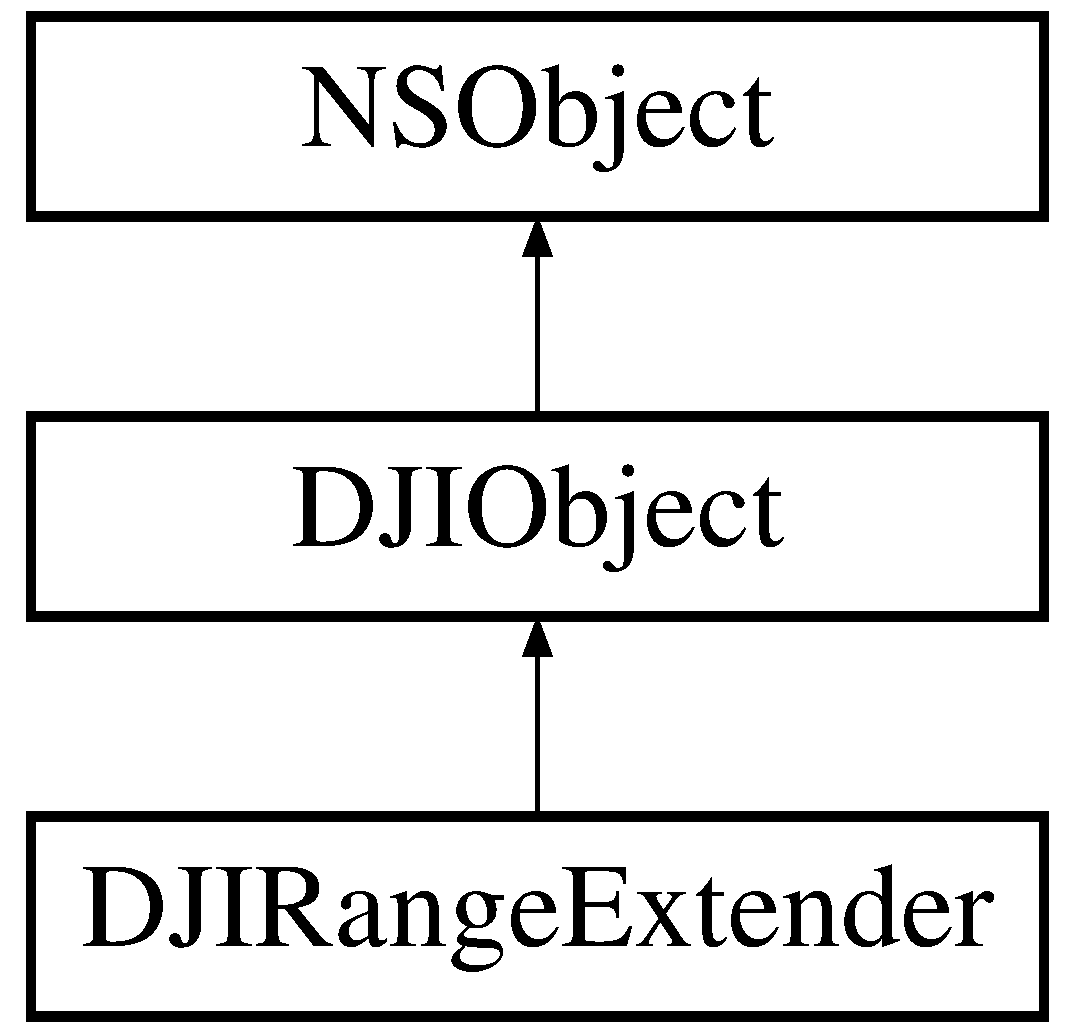
\includegraphics[height=3.000000cm]{interface_d_j_i_range_extender}
\end{center}
\end{figure}
\subsection*{Instance Methods}
\begin{DoxyCompactItemize}
\item 
(int) -\/ \hyperlink{interface_d_j_i_range_extender_a7f37090359acfe02e298062499fc7546}{get\+Range\+Extender\+Power\+Level}
\item 
(B\+O\+O\+L) -\/ \hyperlink{interface_d_j_i_range_extender_aa41f3aaa0e748133963e6d2218442d12}{bind\+Range\+Extender\+With\+Camera\+M\+A\+C\+:camera\+S\+S\+I\+D\+:}
\item 
(N\+S\+String $\ast$) -\/ \hyperlink{interface_d_j_i_range_extender_a0635cd78ebfa3c1c37a1c76f4e909c42}{get\+Current\+Binding\+M\+A\+C}
\item 
(N\+S\+String $\ast$) -\/ \hyperlink{interface_d_j_i_range_extender_afbc8f1859cd7b83bb38270315e9c6fab}{get\+Current\+Binding\+S\+S\+I\+D}
\item 
(N\+S\+String $\ast$) -\/ \hyperlink{interface_d_j_i_range_extender_a8e2824ec831b529771fccedc6a50df4c}{get\+Mac\+Address\+Of\+Range\+Extender}
\item 
(N\+S\+String $\ast$) -\/ \hyperlink{interface_d_j_i_range_extender_a816a8dcd993c99f4fd54b5e59b893c83}{get\+Ssid\+Of\+Range\+Extender}
\item 
(B\+O\+O\+L) -\/ \hyperlink{interface_d_j_i_range_extender_afab6f3806396e27c74a3375b49c5fdf5}{rename\+Ssid\+Of\+Range\+Extender\+:}
\item 
(N\+S\+String $\ast$) -\/ \hyperlink{interface_d_j_i_range_extender_ad34805f00181d4a3e3dba96214f62fd8}{get\+Range\+Extender\+Wi\+Fi\+Password}
\item 
(B\+O\+O\+L) -\/ \hyperlink{interface_d_j_i_range_extender_aab8f7692b11f4e279542aa0890003131}{set\+Range\+Extender\+Wi\+Fi\+Password\+:}
\end{DoxyCompactItemize}


\subsection{Method Documentation}
\hypertarget{interface_d_j_i_range_extender_aa41f3aaa0e748133963e6d2218442d12}{\index{D\+J\+I\+Range\+Extender@{D\+J\+I\+Range\+Extender}!bind\+Range\+Extender\+With\+Camera\+M\+A\+C\+:camera\+S\+S\+I\+D\+:@{bind\+Range\+Extender\+With\+Camera\+M\+A\+C\+:camera\+S\+S\+I\+D\+:}}
\index{bind\+Range\+Extender\+With\+Camera\+M\+A\+C\+:camera\+S\+S\+I\+D\+:@{bind\+Range\+Extender\+With\+Camera\+M\+A\+C\+:camera\+S\+S\+I\+D\+:}!D\+J\+I\+Range\+Extender@{D\+J\+I\+Range\+Extender}}
\subsubsection[{bind\+Range\+Extender\+With\+Camera\+M\+A\+C\+:camera\+S\+S\+I\+D\+:}]{\setlength{\rightskip}{0pt plus 5cm}-\/ (B\+O\+O\+L) bind\+Range\+Extender\+With\+Camera\+M\+A\+C\+: 
\begin{DoxyParamCaption}
\item[{(N\+S\+String $\ast$)}]{mac\+Addr}
\item[{cameraSSID:(N\+S\+String $\ast$)}]{ssid}
\end{DoxyParamCaption}
}}\label{interface_d_j_i_range_extender_aa41f3aaa0e748133963e6d2218442d12}
Bind mac address to the range extender current connected


\begin{DoxyParams}{Parameters}
{\em camera's} & mac addrese and camera's ssid\\
\hline
\end{DoxyParams}
\begin{DoxyReturn}{Returns}
Retrun Y\+E\+S if bind success. 
\end{DoxyReturn}
\begin{DoxyAttention}{Attention}
If bind success, the range extender will reboot 
\end{DoxyAttention}
\hypertarget{interface_d_j_i_range_extender_a0635cd78ebfa3c1c37a1c76f4e909c42}{\index{D\+J\+I\+Range\+Extender@{D\+J\+I\+Range\+Extender}!get\+Current\+Binding\+M\+A\+C@{get\+Current\+Binding\+M\+A\+C}}
\index{get\+Current\+Binding\+M\+A\+C@{get\+Current\+Binding\+M\+A\+C}!D\+J\+I\+Range\+Extender@{D\+J\+I\+Range\+Extender}}
\subsubsection[{get\+Current\+Binding\+M\+A\+C}]{\setlength{\rightskip}{0pt plus 5cm}-\/ (N\+S\+String$\ast$) get\+Current\+Binding\+M\+A\+C 
\begin{DoxyParamCaption}
{}
\end{DoxyParamCaption}
}}\label{interface_d_j_i_range_extender_a0635cd78ebfa3c1c37a1c76f4e909c42}
Get the binding mac address of the range extender current connected

\begin{DoxyReturn}{Returns}
camera's mac addreess if get success. 
\end{DoxyReturn}
\hypertarget{interface_d_j_i_range_extender_afbc8f1859cd7b83bb38270315e9c6fab}{\index{D\+J\+I\+Range\+Extender@{D\+J\+I\+Range\+Extender}!get\+Current\+Binding\+S\+S\+I\+D@{get\+Current\+Binding\+S\+S\+I\+D}}
\index{get\+Current\+Binding\+S\+S\+I\+D@{get\+Current\+Binding\+S\+S\+I\+D}!D\+J\+I\+Range\+Extender@{D\+J\+I\+Range\+Extender}}
\subsubsection[{get\+Current\+Binding\+S\+S\+I\+D}]{\setlength{\rightskip}{0pt plus 5cm}-\/ (N\+S\+String$\ast$) get\+Current\+Binding\+S\+S\+I\+D 
\begin{DoxyParamCaption}
{}
\end{DoxyParamCaption}
}}\label{interface_d_j_i_range_extender_afbc8f1859cd7b83bb38270315e9c6fab}
Get the binding ssid

\begin{DoxyReturn}{Returns}
bingding camera's ssid 
\end{DoxyReturn}
\hypertarget{interface_d_j_i_range_extender_a8e2824ec831b529771fccedc6a50df4c}{\index{D\+J\+I\+Range\+Extender@{D\+J\+I\+Range\+Extender}!get\+Mac\+Address\+Of\+Range\+Extender@{get\+Mac\+Address\+Of\+Range\+Extender}}
\index{get\+Mac\+Address\+Of\+Range\+Extender@{get\+Mac\+Address\+Of\+Range\+Extender}!D\+J\+I\+Range\+Extender@{D\+J\+I\+Range\+Extender}}
\subsubsection[{get\+Mac\+Address\+Of\+Range\+Extender}]{\setlength{\rightskip}{0pt plus 5cm}-\/ (N\+S\+String$\ast$) get\+Mac\+Address\+Of\+Range\+Extender 
\begin{DoxyParamCaption}
{}
\end{DoxyParamCaption}
}}\label{interface_d_j_i_range_extender_a8e2824ec831b529771fccedc6a50df4c}
get M\+A\+C Address of range extender current connected

\begin{DoxyReturn}{Returns}
M\+A\+C address or nil if failed. 
\end{DoxyReturn}
\hypertarget{interface_d_j_i_range_extender_a7f37090359acfe02e298062499fc7546}{\index{D\+J\+I\+Range\+Extender@{D\+J\+I\+Range\+Extender}!get\+Range\+Extender\+Power\+Level@{get\+Range\+Extender\+Power\+Level}}
\index{get\+Range\+Extender\+Power\+Level@{get\+Range\+Extender\+Power\+Level}!D\+J\+I\+Range\+Extender@{D\+J\+I\+Range\+Extender}}
\subsubsection[{get\+Range\+Extender\+Power\+Level}]{\setlength{\rightskip}{0pt plus 5cm}-\/ (int) get\+Range\+Extender\+Power\+Level 
\begin{DoxyParamCaption}
{}
\end{DoxyParamCaption}
}}\label{interface_d_j_i_range_extender_a7f37090359acfe02e298062499fc7546}
Get the power level of the range extender.

\begin{DoxyReturn}{Returns}
Power level between 0 -\/ 10 
\end{DoxyReturn}
\hypertarget{interface_d_j_i_range_extender_ad34805f00181d4a3e3dba96214f62fd8}{\index{D\+J\+I\+Range\+Extender@{D\+J\+I\+Range\+Extender}!get\+Range\+Extender\+Wi\+Fi\+Password@{get\+Range\+Extender\+Wi\+Fi\+Password}}
\index{get\+Range\+Extender\+Wi\+Fi\+Password@{get\+Range\+Extender\+Wi\+Fi\+Password}!D\+J\+I\+Range\+Extender@{D\+J\+I\+Range\+Extender}}
\subsubsection[{get\+Range\+Extender\+Wi\+Fi\+Password}]{\setlength{\rightskip}{0pt plus 5cm}-\/ (N\+S\+String$\ast$) get\+Range\+Extender\+Wi\+Fi\+Password 
\begin{DoxyParamCaption}
{}
\end{DoxyParamCaption}
}}\label{interface_d_j_i_range_extender_ad34805f00181d4a3e3dba96214f62fd8}
Get wifi password

\begin{DoxyReturn}{Returns}
wifi password or nil 
\end{DoxyReturn}
\hypertarget{interface_d_j_i_range_extender_a816a8dcd993c99f4fd54b5e59b893c83}{\index{D\+J\+I\+Range\+Extender@{D\+J\+I\+Range\+Extender}!get\+Ssid\+Of\+Range\+Extender@{get\+Ssid\+Of\+Range\+Extender}}
\index{get\+Ssid\+Of\+Range\+Extender@{get\+Ssid\+Of\+Range\+Extender}!D\+J\+I\+Range\+Extender@{D\+J\+I\+Range\+Extender}}
\subsubsection[{get\+Ssid\+Of\+Range\+Extender}]{\setlength{\rightskip}{0pt plus 5cm}-\/ (N\+S\+String$\ast$) get\+Ssid\+Of\+Range\+Extender 
\begin{DoxyParamCaption}
{}
\end{DoxyParamCaption}
}}\label{interface_d_j_i_range_extender_a816a8dcd993c99f4fd54b5e59b893c83}
Get S\+S\+I\+D of range extender current connected

\begin{DoxyReturn}{Returns}
ssid 
\end{DoxyReturn}
\hypertarget{interface_d_j_i_range_extender_afab6f3806396e27c74a3375b49c5fdf5}{\index{D\+J\+I\+Range\+Extender@{D\+J\+I\+Range\+Extender}!rename\+Ssid\+Of\+Range\+Extender\+:@{rename\+Ssid\+Of\+Range\+Extender\+:}}
\index{rename\+Ssid\+Of\+Range\+Extender\+:@{rename\+Ssid\+Of\+Range\+Extender\+:}!D\+J\+I\+Range\+Extender@{D\+J\+I\+Range\+Extender}}
\subsubsection[{rename\+Ssid\+Of\+Range\+Extender\+:}]{\setlength{\rightskip}{0pt plus 5cm}-\/ (B\+O\+O\+L) rename\+Ssid\+Of\+Range\+Extender\+: 
\begin{DoxyParamCaption}
\item[{(N\+S\+String $\ast$)}]{new\+Ssid}
\end{DoxyParamCaption}
}}\label{interface_d_j_i_range_extender_afab6f3806396e27c74a3375b49c5fdf5}
Rename the extender's ssid.


\begin{DoxyParams}{Parameters}
{\em new\+Name} & new ssid name of range extender, must has prefix \char`\"{}\+Phantom\+\_\+\char`\"{} \\
\hline
\end{DoxyParams}
\begin{DoxyAttention}{Attention}
if rename success, the range extender will reboot 
\end{DoxyAttention}
\hypertarget{interface_d_j_i_range_extender_aab8f7692b11f4e279542aa0890003131}{\index{D\+J\+I\+Range\+Extender@{D\+J\+I\+Range\+Extender}!set\+Range\+Extender\+Wi\+Fi\+Password\+:@{set\+Range\+Extender\+Wi\+Fi\+Password\+:}}
\index{set\+Range\+Extender\+Wi\+Fi\+Password\+:@{set\+Range\+Extender\+Wi\+Fi\+Password\+:}!D\+J\+I\+Range\+Extender@{D\+J\+I\+Range\+Extender}}
\subsubsection[{set\+Range\+Extender\+Wi\+Fi\+Password\+:}]{\setlength{\rightskip}{0pt plus 5cm}-\/ (B\+O\+O\+L) set\+Range\+Extender\+Wi\+Fi\+Password\+: 
\begin{DoxyParamCaption}
\item[{(N\+S\+String $\ast$)}]{password}
\end{DoxyParamCaption}
}}\label{interface_d_j_i_range_extender_aab8f7692b11f4e279542aa0890003131}
set wifi password


\begin{DoxyParams}{Parameters}
{\em password} & New wifi passwords that is made up of letters and numbers and should be 8 -\/ 16 characters。 set nil to cancel setup password \\
\hline
\end{DoxyParams}
\begin{DoxyAttention}{Attention}
Hard reset range extender will clean password 
\end{DoxyAttention}


The documentation for this class was generated from the following file\+:\begin{DoxyCompactItemize}
\item 
D\+J\+I\+Range\+Extender.\+h\end{DoxyCompactItemize}

\hypertarget{protocol_d_j_i_s_d_card_operation-p}{\section{$<$D\+J\+I\+S\+D\+Card\+Operation$>$ Protocol Reference}
\label{protocol_d_j_i_s_d_card_operation-p}\index{$<$\+D\+J\+I\+S\+D\+Card\+Operation$>$@{$<$\+D\+J\+I\+S\+D\+Card\+Operation$>$}}
}
Inheritance diagram for $<$D\+J\+I\+S\+D\+Card\+Operation$>$\+:\begin{figure}[H]
\begin{center}
\leavevmode
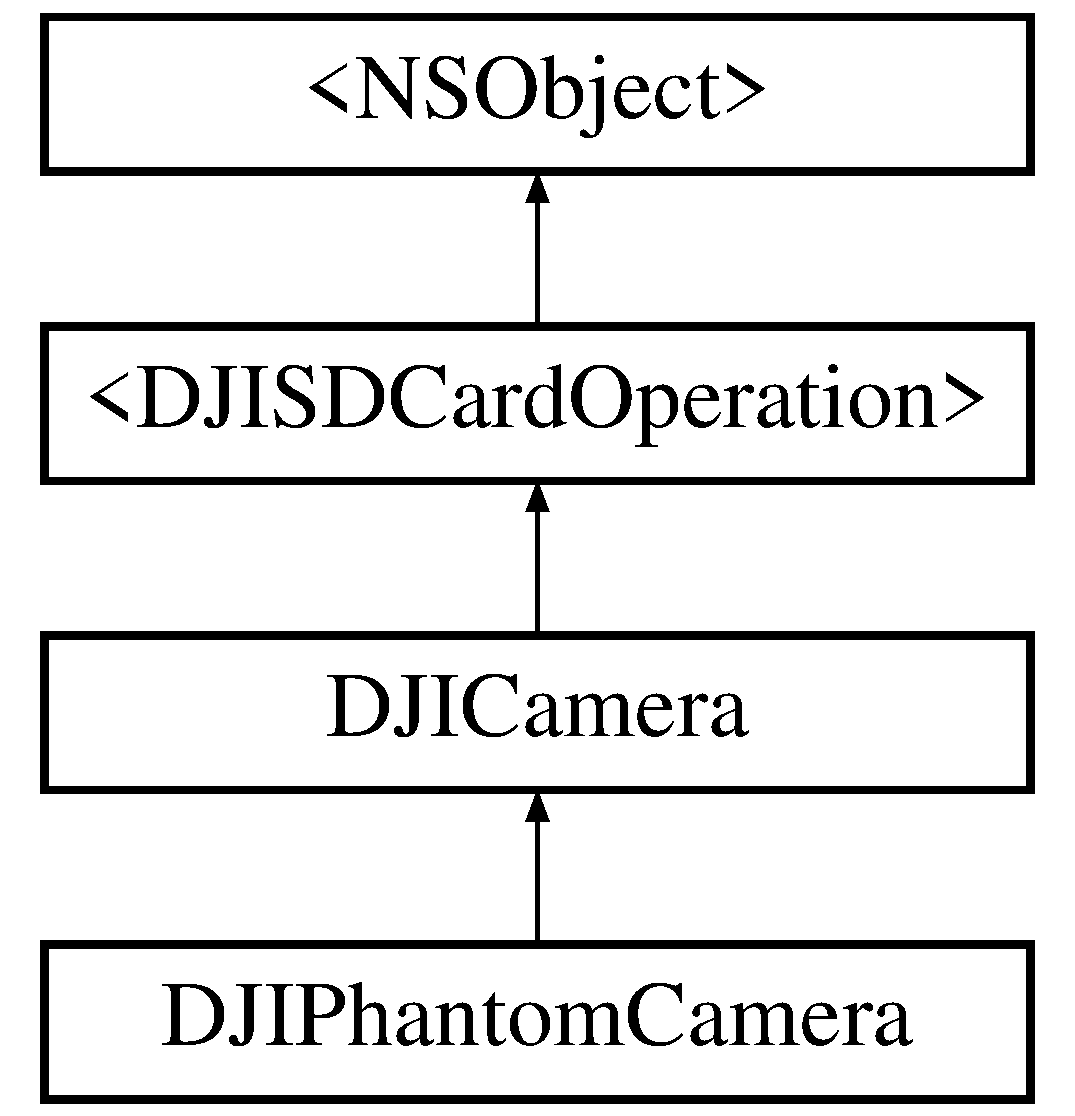
\includegraphics[height=4.000000cm]{protocol_d_j_i_s_d_card_operation-p}
\end{center}
\end{figure}
\subsection*{Instance Methods}
\begin{DoxyCompactItemize}
\item 
(void) -\/ \hyperlink{protocol_d_j_i_s_d_card_operation-p_a41de4b36a3b57eecab4c6ac34d36b794}{format\+S\+D\+Card\+:}
\item 
(void) -\/ \hyperlink{protocol_d_j_i_s_d_card_operation-p_a3f35e575f0ae0f34f32b6b14ce98f22c}{get\+S\+D\+Card\+Info\+:}
\end{DoxyCompactItemize}


\subsection{Method Documentation}
\hypertarget{protocol_d_j_i_s_d_card_operation-p_a41de4b36a3b57eecab4c6ac34d36b794}{\index{D\+J\+I\+S\+D\+Card\+Operation-\/p@{D\+J\+I\+S\+D\+Card\+Operation-\/p}!format\+S\+D\+Card\+:@{format\+S\+D\+Card\+:}}
\index{format\+S\+D\+Card\+:@{format\+S\+D\+Card\+:}!D\+J\+I\+S\+D\+Card\+Operation-\/p@{D\+J\+I\+S\+D\+Card\+Operation-\/p}}
\subsubsection[{format\+S\+D\+Card\+:}]{\setlength{\rightskip}{0pt plus 5cm}-\/ (void) format\+S\+D\+Card\+: 
\begin{DoxyParamCaption}
\item[{(D\+J\+I\+Execute\+Result\+Block)}]{block}
\end{DoxyParamCaption}
}}\label{protocol_d_j_i_s_d_card_operation-p_a41de4b36a3b57eecab4c6ac34d36b794}
Format S\+D card


\begin{DoxyParams}{Parameters}
{\em block} & Remote execute result block. \\
\hline
\end{DoxyParams}
\hypertarget{protocol_d_j_i_s_d_card_operation-p_a3f35e575f0ae0f34f32b6b14ce98f22c}{\index{D\+J\+I\+S\+D\+Card\+Operation-\/p@{D\+J\+I\+S\+D\+Card\+Operation-\/p}!get\+S\+D\+Card\+Info\+:@{get\+S\+D\+Card\+Info\+:}}
\index{get\+S\+D\+Card\+Info\+:@{get\+S\+D\+Card\+Info\+:}!D\+J\+I\+S\+D\+Card\+Operation-\/p@{D\+J\+I\+S\+D\+Card\+Operation-\/p}}
\subsubsection[{get\+S\+D\+Card\+Info\+:}]{\setlength{\rightskip}{0pt plus 5cm}-\/ (void) get\+S\+D\+Card\+Info\+: 
\begin{DoxyParamCaption}
\item[{(void($^\wedge$)({\bf D\+J\+I\+Camera\+S\+D\+Card\+Info} $\ast$sd\+Info, {\bf D\+J\+I\+Error} $\ast$error))}]{block}
\end{DoxyParamCaption}
}}\label{protocol_d_j_i_s_d_card_operation-p_a3f35e575f0ae0f34f32b6b14ce98f22c}
Get S\+D card information and status


\begin{DoxyParams}{Parameters}
{\em block} & Remote execute result block. \\
\hline
\end{DoxyParams}


The documentation for this protocol was generated from the following file\+:\begin{DoxyCompactItemize}
\item 
D\+J\+I\+S\+D\+Card\+Operation.\+h\end{DoxyCompactItemize}

\hypertarget{interface_ground_station_execute_result}{\section{Ground\+Station\+Execute\+Result Class Reference}
\label{interface_ground_station_execute_result}\index{Ground\+Station\+Execute\+Result@{Ground\+Station\+Execute\+Result}}
}
Inheritance diagram for Ground\+Station\+Execute\+Result\+:\begin{figure}[H]
\begin{center}
\leavevmode
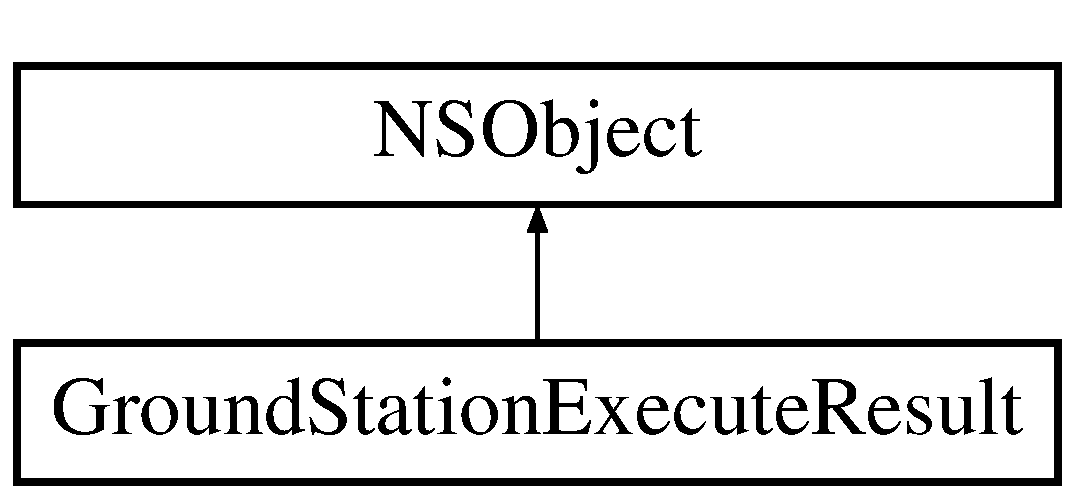
\includegraphics[height=2.000000cm]{interface_ground_station_execute_result}
\end{center}
\end{figure}
\subsection*{Instance Methods}
\begin{DoxyCompactItemize}
\item 
\hypertarget{interface_ground_station_execute_result_aed506ad3e7e9e0be36278fe0707e397f}{(id) -\/ {\bfseries init\+With\+Action\+:}}\label{interface_ground_station_execute_result_aed506ad3e7e9e0be36278fe0707e397f}

\end{DoxyCompactItemize}
\subsection*{Properties}
\begin{DoxyCompactItemize}
\item 
G\+S\+Action\+Type \hyperlink{interface_ground_station_execute_result_aed74c158994195c5f0ac2bdb0577b02e}{current\+Action}
\item 
G\+S\+Execute\+Status \hyperlink{interface_ground_station_execute_result_ab3cb1e15e2841548938ce23f1bacc612}{execute\+Status}
\item 
G\+S\+Error \hyperlink{interface_ground_station_execute_result_a3bf529c213113e8f28264e9d50228425}{error}
\end{DoxyCompactItemize}


\subsection{Property Documentation}
\hypertarget{interface_ground_station_execute_result_aed74c158994195c5f0ac2bdb0577b02e}{\index{Ground\+Station\+Execute\+Result@{Ground\+Station\+Execute\+Result}!current\+Action@{current\+Action}}
\index{current\+Action@{current\+Action}!Ground\+Station\+Execute\+Result@{Ground\+Station\+Execute\+Result}}
\subsubsection[{current\+Action}]{\setlength{\rightskip}{0pt plus 5cm}-\/ (G\+S\+Action\+Type) current\+Action\hspace{0.3cm}{\ttfamily [read]}, {\ttfamily [write]}, {\ttfamily [nonatomic]}, {\ttfamily [assign]}}}\label{interface_ground_station_execute_result_aed74c158994195c5f0ac2bdb0577b02e}
Current executing action \hypertarget{interface_ground_station_execute_result_a3bf529c213113e8f28264e9d50228425}{\index{Ground\+Station\+Execute\+Result@{Ground\+Station\+Execute\+Result}!error@{error}}
\index{error@{error}!Ground\+Station\+Execute\+Result@{Ground\+Station\+Execute\+Result}}
\subsubsection[{error}]{\setlength{\rightskip}{0pt plus 5cm}-\/ (G\+S\+Error) error\hspace{0.3cm}{\ttfamily [read]}, {\ttfamily [write]}, {\ttfamily [nonatomic]}, {\ttfamily [assign]}}}\label{interface_ground_station_execute_result_a3bf529c213113e8f28264e9d50228425}
Error \hypertarget{interface_ground_station_execute_result_ab3cb1e15e2841548938ce23f1bacc612}{\index{Ground\+Station\+Execute\+Result@{Ground\+Station\+Execute\+Result}!execute\+Status@{execute\+Status}}
\index{execute\+Status@{execute\+Status}!Ground\+Station\+Execute\+Result@{Ground\+Station\+Execute\+Result}}
\subsubsection[{execute\+Status}]{\setlength{\rightskip}{0pt plus 5cm}-\/ (G\+S\+Execute\+Status) execute\+Status\hspace{0.3cm}{\ttfamily [read]}, {\ttfamily [write]}, {\ttfamily [nonatomic]}, {\ttfamily [assign]}}}\label{interface_ground_station_execute_result_ab3cb1e15e2841548938ce23f1bacc612}
Execute status 

The documentation for this class was generated from the following file\+:\begin{DoxyCompactItemize}
\item 
D\+J\+I\+Ground\+Station.\+h\end{DoxyCompactItemize}

%--- End generated contents ---

% Index
\newpage
\phantomsection
\addcontentsline{toc}{chapter}{Index}
\printindex

\end{document}
